\documentclass[11pt,a4paper,twoside]{book}

%encoding
\usepackage[utf8]{inputenc}
\usepackage[T1]{fontenc}

\usepackage{amsmath}
\usepackage{mathtools}
\usepackage{amstext}
\usepackage{amsfonts}
\usepackage{amssymb}
\usepackage{graphicx}
\usepackage{longtable}
\usepackage{booktabs}
\usepackage[bookmarks=true,colorlinks=true,urlcolor=blue,citecolor=blue,linkcolor=blue,unicode=true]{hyperref}
\usepackage[top=2.5cm, bottom=2.5cm, bindingoffset=0.5cm, margin=2.5cm]{geometry}
\usepackage{siunitx}

\setlength{\parindent}{0pt}
\setlength{\parskip}{6pt plus 2pt minus 1pt}
\setlength{\emergencystretch}{3em}  % prevent overfull lines
\providecommand{\tightlist}{%
  \setlength{\itemsep}{0pt}\setlength{\parskip}{0pt}}

% pandoc does not parse latex environment
% for landscape tables
\usepackage{lscape}
\usepackage{pdfpages}
\newcommand{\blandscape}{\begin{landscape}}
\newcommand{\elandscape}{\end{landscape}}

%predefined commands
\newcommand{\Cb}{C_\beta} 
\newcommand{\eq}{\!=\!} 
\newcommand{\Gauss}{\mathcal{N}} 
\renewcommand{\H}{\mathbf{H}} 
\newcommand{\Hij}{\H_{ij}} 
\newcommand{\I}{\mathbf{I}} 
\newcommand{\Lijk}{\mathbf{\Lambda}_{ij,k}}
\newcommand{\Lk}{\mathbf{\Lambda}_k}
\newcommand{\LL}{L\!L(\mathbf{v}, \mathbf{w})}
\newcommand{\LLreg}{L\!L_\mathrm{reg}}
\newcommand{\muijk}{\mathbf{\mu}_{ij,k}}
\newcommand{\muk}{\mathbf{\mu}_k}
\newcommand{\neff}{N_\mathrm{eff}}
\renewcommand{\r}{\mathbf{r}}
\renewcommand{\c}{\mathbf{c}}
\newcommand{\rij}{r_{ij}}
\newcommand{\cij}{c_{ij}}
\newcommand{\seq}{\mathbf{x}}
\newcommand{\Qij}{\mathbf{Q}_{ij}}
\newcommand{\q}{\mathbf{q}}
\newcommand{\qij}{\mathbf{q\prime}_{ij}}
\newcommand{\Sn}{S_n}
\renewcommand{\v}{\mathbf{v}}
\newcommand{\vi}{v_{i}}
\newcommand{\vj}{v_{j}}
\newcommand{\via}{v_{ia}}
\newcommand{\vja}{v_{ja}}
\newcommand{\w}{\mathbf{w}}
\newcommand{\wij}{\mathbf{w}_{ij}}
\newcommand{\wijab}{w_{ijab}}
\newcommand{\wijcd}{w_{ijcd}}
\newcommand{\wklcd}{w_{klcd}}
\newcommand{\X}{\mathbf{X}}
\newcommand{\angstrom}{\mathring{A} \;}


% Numbering of sections unto depth=5
\setcounter{secnumdepth}{5}

% Table of contents formatting
\renewcommand{\contentsname}{Table of Contents}
\setcounter{tocdepth}{1}

% Headers and page numbering 
\usepackage{fancyhdr}
\pagestyle{plain}

% Chapter styling
\usepackage[grey]{quotchap}
\makeatletter 
\renewcommand*{\chapnumfont}{%
  \usefont{T1}{\@defaultcnfont}{b}{n}\fontsize{80}{100}\selectfont% Default: 100/130
  \color{chaptergrey}%
}
\makeatother


%------------------- Definition of LMU title pages
\newcommand{\LMUCover}[3]{
    \thispagestyle{empty}
    {\parindent0cm \rule{\linewidth}{.7ex}}
    
    \begin{flushright}
      \vspace*{\stretch{1}}
      \sffamily\bfseries\Huge
      #1\\
      \vspace*{\stretch{1}}
      \sffamily\bfseries\large
      #2
      \vspace*{\stretch{1}}
    \end{flushright}
  
    \rule{\linewidth}{.7ex}
    \vspace*{\stretch{5}}
    \vspace*{\stretch{1}}
    
    \begin{center}\sffamily\LARGE{#3}\end{center}
}



\newcommand{\LMUTitlePage}[4]{
    \thispagestyle{empty}
    \vspace*{\stretch{1}}
    
    \begin{center}
      \Large Dissertation zur Erlangung des Doktorgrades der Fakultät für Chemie und Pharmazie der Ludwig-Maximilians-Universität München
    \end{center}
    
    \vspace*{\stretch{1}}
    {\parindent0cm \rule{\linewidth}{.7ex}}
    
    \begin{flushright}
      \vspace*{\stretch{1}}
      \sffamily\bfseries\Huge
      #1\\
      \vspace*{\stretch{1}}
    \end{flushright}
  
    \rule{\linewidth}{.7ex}

    \vspace*{\stretch{3}}
    \begin{center}
      \Large vorgelegt von\\
      \Large #2\\
      \Large geboren in #3\\
      \vspace*{\stretch{2}}
      \Large München, den #4
    \end{center}
}


\newcommand{\LMUErklaerung}[5]{
    \thispagestyle{empty}
    \begin{flushleft}
      \large \textbf{Erklärung} \\[1mm]
      \large Diese Dissertation wurde im Sinne von §7 der Promotionsordnung vom 28. November 2011 von #2 betreut.
      \bigskip
  
      \large \textbf{Eidesstattliche Versicherung}\\[1mm]
      \large Diese Dissertation wurde eigenständig und ohne unerlaubte Hilfe erarbeitet.
      \vspace{5em}
  
      \dots\dots\dots   \dots\dots\dots \hfill \dots\dots\dots\dots\dots\dots\dots\dots\\
      \large Ort, Datum \hfill #1
      \vfill
  
  
      \large Dissertation eingereicht am: \hfill #4
      \bigskip
    
      \large Erstgutachter:  #2 \hfill \dots\dots\dots\dots\dots\dots\dots
      \bigskip
    
      \large Zweitgutachter: #3 \hfill \dots\dots\dots\dots\dots\dots\dots
      \bigskip
    
      \large Tag der mündlichen Prüfung: \hfill #5
    \end{flushleft}
}


\usepackage{amsthm}
\newtheorem{theorem}{Theorem}[chapter]
\newtheorem{lemma}{Lemma}[chapter]
\theoremstyle{definition}
\newtheorem{definition}{Definition}[chapter]
\newtheorem{corollary}{Corollary}[chapter]
\newtheorem{proposition}{Proposition}[chapter]
\theoremstyle{definition}
\newtheorem{example}{Example}[chapter]
\theoremstyle{remark}
\newtheorem*{remark}{Remark}
\begin{document}

\frontmatter

%%% LMU cover page
\LMUCover
	{Bayesian Model for Prediction of Protein Residue-Residue Contacts}
	{Susann Vorberg}
	{15.10.2017}

\newpage
\thispagestyle{empty}
\cleardoublepage

%%% LMU title page
\LMUTitlePage
	{Bayesian Model for Prediction of Protein Residue-Residue Contacts}
	{Susann Vorberg}
	{Leipzig, Germany}
	{15.10.2017}

\newpage
\thispagestyle{empty}
\cleardoublepage

%%% LMU statement page
\LMUErklaerung
	{Susann Vorberg}
	{Dr. Johannes Soeding}
	{Prof. Dr. Julien Gagneur}
	{15.10.2017}
	{15.12.2017}

\newpage
\thispagestyle{empty}
\cleardoublepage
\frontmatter\setcounter{page}{1}

\chapter*{Summary}\label{summary}
\addcontentsline{toc}{chapter}{Summary}

Despite tremendous efforts in automating experimental structure
prediction and systematical target selection in structural genomics
projects, the gap between the number of protein sequences and solved
protein structures is constantly widening. While high-throughput DNA
sequencing technologies are advancing at an extraordinary pace, thereby
not only decreasing the amount of time needed to sequence whole genomes
but also drastically reducing costs, experimental techniques for
structure determination are still labour intensive, time-consuming and
very expensive. This trend illustrates the essential importance of
computational approaches that can complement experimental structural
biology efforts in order to bridge the sequence-structure gap.

About half of the known protein families are annotated with experimental
structural data and most likely are eligible for template-based
structure prediction by which the protein structure is inferred from
experimentally solved structures of homologous proteins. The other half
can theoratically be addressed by \emph{de novo} structure prediction
methods that minimize physical or knowledge based energy functions to
identify the lowest-energy conformation that generally corresponds to
the native protein conformation. However, in practice these approaches
are limited by the immense computational costs to search the space of
possible conformations.

Recent advancements in residue-residue contact prediction have enabled
the \emph{de novo} prediction of protein structures by constraining the
overall protein fold and thereby reducing the conformational search
space sufficiently. Residue-residue contact prediction is based on the
old idea that spatially proximate amino acid residues tend to coevolve,
leaving an echo of correlations in the evolutionary record. The
predicted contacts can not only be used to guide \emph{de novo}
structure prediction but they have also been successfully applied in
diverse biological fields, such as predicting residue interactions in
protein interfaces, studying protein flexibility and alternative
conformations, quantifying the effects of mutations and ranking and
validation of structural models.

Despite the immense success of the new generation of contact prediction
methods, several open challeges need to be addresed to broaden their
applicability. The most evident limitation lies in the requirement of
deep alignments that amplify the coevolutionary signal. Unfortunately,
the most interesting targets for contact prediction, being protein
families without any associated structural information, comprise low
numbers of homologous sequences. Furthermore, the current methods apply
heuristics that leave certain aspects of the available coevolutionary
information unexploited but have so far resisted efforts to replace
them.

This work aims to improve the sensitivity of residue-residue contact
prediction methods by exploiting the full coevolutionary information in
a principled Bayesian framework. The statistical model underlying the
current contact prediction approaches is embedded into the Bayesian
framework which allows to deliver posterior estimates of contact
probabilities instead of heuristic contact scores. The explicit
modelling of amino acid preferences concealed in the coevolutionary
coupling signal reflects the nature of residue-residue interactions.
Furthermore,the Bayesian framework can naturally be extended to derive
estimates of the probability distributions of the distances between
residue pairs, which will be the focus of future work.

\chapter*{Acknowledgements}\label{acknowledgements}
\addcontentsline{toc}{chapter}{Acknowledgements}

I thank the world.

\tableofcontents
\addcontentsline{toc}{chapter}{Table of Contents}

\mainmatter \setcounter{page}{1}

\chapter{Biological Background}\label{general-intro}

In 1972, Anfinsen and his collegues received the Nobel Prize for their
research on protein folding which lead to the postulation of one of the
basic principles in molecular biology, which is known as
\emph{Anfinsen's dogma}: a protein's native structure is uniquely
determined by its amino acid sequence
{[}\protect\hyperlink{ref-Anfinsen1973}{1}{]}. With certain exceptions
(e.g.~intrinsically disordered proteins
{[}\protect\hyperlink{ref-Wright1999}{2}{]},
prions{[}\protect\hyperlink{ref-Fraser2014}{3}{]}), this dogma has
proven to hold true at least for globular proteins.

Ever since, it is regarded as the biggest challenge in structural
bioinformatics to realiably predict a protein's structure given only its
amino acid sequence
{[}\protect\hyperlink{ref-Samish2015}{4},\protect\hyperlink{ref-Schwede2013}{5}{]}.
\emph{De~novo} protein structure prediction methods minimize physical or
knowledge based energy functions to identify the lowest-energy
conformation that generally corresponds to the native protein
conformation. However, due to the high degree of conformational
flexibility, the search space of possible conformations cannot be
explored exhaustively for proteins of typical length. Given a protein
with 101 residues that has 100 peptide bonds with two torsion angles
each and assuming three stable conformations for each of the bond
angles, there will be \(3^200 \approx 10^{95}\) configurations. This
number of conformations cannot be sampled sequentially in a lifetime,
even when sampling at high rates. Yet, proteins fold almost
instantaneously within milliseconds. This discrepancy is known as
Levinthal's paradox {[}\protect\hyperlink{ref-Levinthal1969}{6}{]} and
limits purely \emph{de novo} based protein structure prediction to small
proteins.

Far more successfull are template-based modelling approaches. Given the
observation that structure is more conserved than sequence in a protein
family {[}\protect\hyperlink{ref-Lesk1980}{7}{]}, the structure of a
target protein can be inferred from a homologue protein
{[}\protect\hyperlink{ref-Sander1991}{8}{]}. The degree of structural
conservation is linked to the level of pairwise sequence identity
{[}\protect\hyperlink{ref-Chothia1986}{9}{]}. Therefore, the accuracy of
a model crucially depends on the sequence identity between target and
template and determines the applicability of the model
{[}\protect\hyperlink{ref-Marti-Renom2000}{10}{]}. By definition,
homology derived models are unable to capture new folds and their main
limitation lies in the availability and identification of suitable
templates {[}\protect\hyperlink{ref-Dorn2014}{11}{]}.

The number of solved protein structures increases steadily but only
slowly, as experimental methods are both time consuming and expensive
{[}\protect\hyperlink{ref-Dorn2014}{11}{]}. The
\protect\hyperlink{abbrev}{PDB}{[}\protect\hyperlink{ref-Berman2000}{12}{]}
is the main repository for marcomolecular structures and currently
(October 2017) holds about 135,000 atomic models of proteins. The
primary technique for determining protein structures is X-ray
crystallography, accounting for roughly 90\% of entries in the
\protect\hyperlink{abbrev}{PDB}. About 9\% of protein structures have
been solved using \protect\hyperlink{abbrev}{NMR} and less than 1\%
using \protect\hyperlink{abbrev}{EM} (see left plot in Figure
\ref{fig:seq-str-gap}).












\begin{figure}
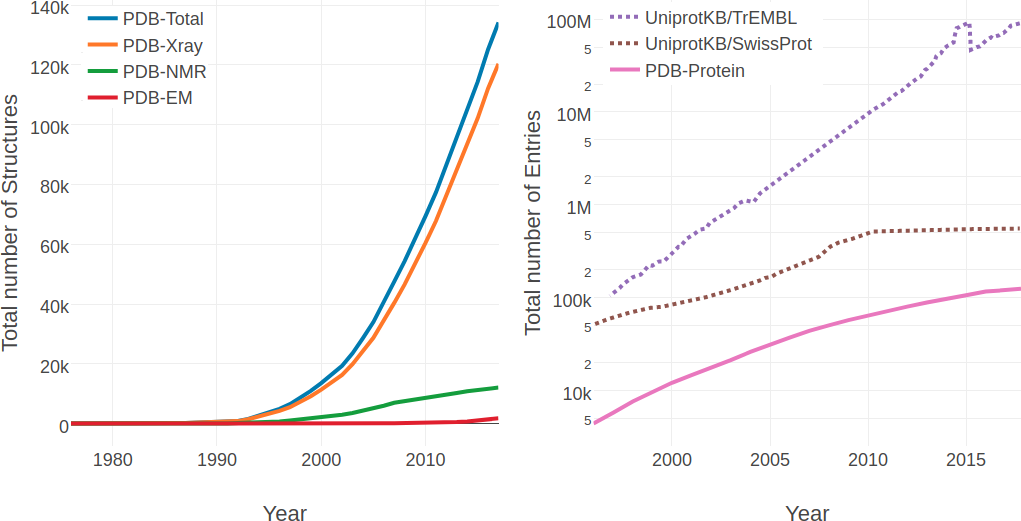
\includegraphics[width=1\linewidth]{img/intro/pdb_uniprot_stats} \caption{Yearly growth of number of solved structures
in the \protect\hyperlink{abbrev}{PDB}
{[}\protect\hyperlink{ref-Berman2000}{12}{]} and protein sequences in
the Uniprot {[}\protect\hyperlink{ref-TheUniProtConsortium2017}{13}{]}.
\textbf{Left} Yearly growth of structures in PDB by structure
determination method. \textbf{Right} Yearly growth of protein sequences
in the UniprotKB/TrEMBL, containing automatically annotated sequences,
and in the UniprotKB/SwissProt, which is curated by experts who
critically review experimental and predicted, and protein structures in
the \protect\hyperlink{abbrev}{PDB}.}\label{fig:seq-str-gap}
\end{figure}

All three experimental techniques have advantages and limitations with
respect to certain modelling aspects. X-ray crystallography involves
protein overexpression, purification and crystallization and finding the
the correct experimental conditions to arrive at a pure and regular
crystal is a challenging and sometimes impossible task. Especially
membrane proteins are difficult to study owing to their overall
flexibility and hydrophobic surfaces which requires suitable detergents
to extract the proteins from their membrane environment which in turn
makes crystallization even more challenging
{[}\protect\hyperlink{ref-Carpenter2008}{14},\protect\hyperlink{ref-Moraes2014}{15}{]}.
Furthermore, the unnatural crystal environment can result in
crystal-induced artifacts, like altererd sidechain conformations due to
crystal packing interactions
{[}\protect\hyperlink{ref-Jacobson2002}{16}{]}. In contrast, Nuclear
magnetic resonance (NMR) spectroscopy studies the protein in solution
under physiological conditions and enables the observation of
intramolecular dynamics, reaction kinetics or protein folding as
ensembles of protein structures can be observed
{[}\protect\hyperlink{ref-Bieri2011}{17}{]}. On the downside, validation
of NMR-derived structure ensembles is complicated and there is an upper
size limit of about 25 kDa for efficient use of the technique
{[}\protect\hyperlink{ref-Billeter2008}{18}{]}. Recently, cryo-EM has
undergone a ``resolution revolution'' and macromolecules have been
solved to near-atomic resolutions
{[}\protect\hyperlink{ref-Egelman2016}{19},\protect\hyperlink{ref-Fernandez-Leiro2016}{20}{]}.
Technological developments, such as better electron detectors as well as
advanced image processing software has enabled high resolution structure
determination and led to an exponential growth in number of structures
deposited in the PDB. Cryo-EM is particularly suited to study large
macromolecular complexes without the need to make crystals and therefore
complements the other two structure determination techniques.

In contrast to the tedious task of determining the tertiary structure of
a protein to atomic resolution, it has become very easy to decipher the
primary sequence of proteins. Since the completion of the human genome
in 2003, high-throughput sequencing technologies have been developed at
an extraordinary pace, thereby not only decreasing the amount of time
needed to sequence whole genomes but also drastically reducing costs
{[}\protect\hyperlink{ref-Reuter2015}{21}{]}. The price for sequencing a
single genome has dropped from the US\$3 billion spent by the Human
Genome Project to as little as
US\$1,000{[}\protect\hyperlink{ref-Goodwin2016}{22}{]}. At the beginning
of 2017, Illumina announced the launch of their latest high-throughput
sequencing technology, NovaSeq, which is capable of sequencing
\(\sim \! 48\) human genomes in parallel at 30x coverage within
\textasciitilde{}45hours
{[}\protect\hyperlink{ref-NovaSeqSystemSpecifications}{23}{]}. Advances
in sequencing technologies have led to the emergence of new fields of
studies, like metagenomics and single-cell genomics, that enable
sequencing of microorganisms that cannot be cultured in a lab
{[}\protect\hyperlink{ref-Tringe2005}{24}--\protect\hyperlink{ref-Wooley2010}{26}{]}.
With these approaches the genomic coverage of the microbial world is
expanding which is directly reflected in a substantial increase in novel
protein families
{[}\protect\hyperlink{ref-Rinke2013}{27}--\protect\hyperlink{ref-Forster2017}{29}{]}.
About 90 million sequences (October 2017) have been translated into
protein amino acid sequences and are stored in the UniprotKB/TrEMBL
database, the leading resource for protein sequences
{[}\protect\hyperlink{ref-TheUniProtConsortium2017}{13}{]}.

The resultant gap between the number of protein structures and protein
sequences is constantly widening (see right plot in Figure
\ref{fig:seq-str-gap}) despite tremendous efforts in automating
experimental structure determination and new developments such as
electron
crystallography{[}\protect\hyperlink{ref-Schwede2013}{5},\protect\hyperlink{ref-Clabbers2017}{30}{]}.
This trend illustrates the essential importance of computational
approaches that can complement experimental structural biology efforts
in order to bridge this gap. Over the last decades, template-based
methods have matured to a point where they are able to generate
high-resolution structural models that are routinley and conveniently
used in life-science research and by the biological community
{[}\protect\hyperlink{ref-Schwede2013}{5},\protect\hyperlink{ref-BKC2016}{31}{]}.
\emph{De novo} methods aiming at predicting protein structures from
sequence alone are required in case no homologue template structure can
be identified or the protein sequence represents a novel fold. Albeit
purely \emph{de novo} approaches are hampered by the combinatorial
explosion of possible conformations for larger proteins, combining them
with structural information from heterogenous sources can help to reduce
the degrees of freedom in the conformational search space
{[}\protect\hyperlink{ref-Schwede2013}{5}{]}. For example, sparse
low-resolution experimental data from chemical cross-linking/mass
spectroscopy or nuclear Overhauser enhancement (NOE) distance data
generated from \protect\hyperlink{abbrev}{NMR} experiments, provide
distance restraints to guide folding to a correct structure
{[}\protect\hyperlink{ref-Li2004}{32}--\protect\hyperlink{ref-Rappsilber2011}{34}{]}.
Sophisticated integrative approaches, exploiting structural information
from different types of experiments have proven to be a powerful
approach
{[}\protect\hyperlink{ref-Ornes2016}{35}--\protect\hyperlink{ref-Tang2015}{37}{]}.













\begin{figure}

{\centering 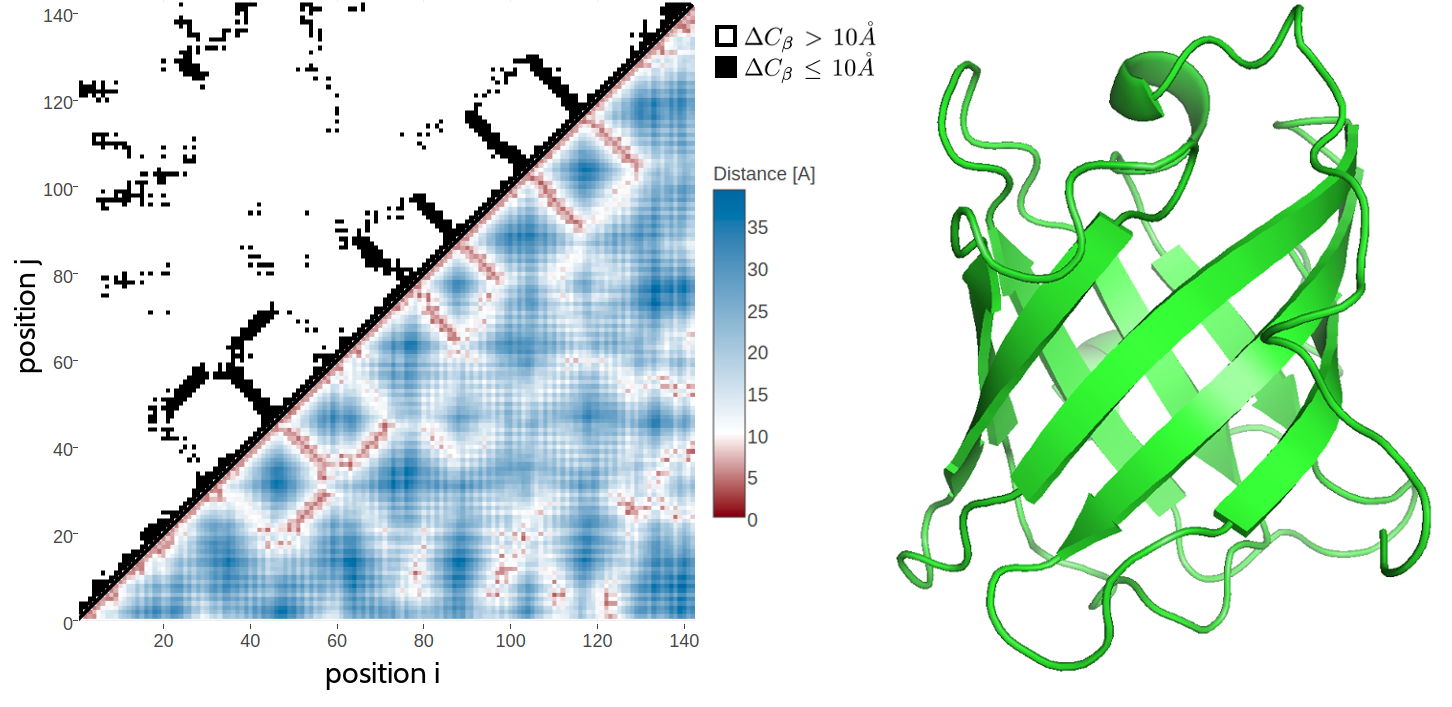
\includegraphics[width=1\linewidth]{img/intro/contat_map_and_structure_1avgi00} 

}

\caption{2D and 3D representations of triabin, a
thombin inhibitor from triatoma pallidipennis (PDB identifier 1avg chain
I). \textbf{Left} The upper left matrix illustrates a contact map using
an \(10 \angstrom \Cb\) cutoff. A black square is drawn at position
\((i, j)\) if the \(\Cb\) atoms of residues \(i\) and \(j\) are closer
than \(8 \angstrom\) in the structure. The lower right matrix
illustrates a distance map. Color reflects \(\Cb\) distances between
residue pairs with red colors representing
\(\Delta \Cb \le 10 \angstrom\) and blue colors representing
\(\Delta \Cb > 10 \angstrom\). \textbf{Right} 3D Structure showing an
eight-stranded beta-barrel.}\label{fig:contact-map}
\end{figure}

Recently, computational methods have been developed using co-evolution
information from deep multiple sequence alignments to predict contacts
between pairs of amino acid residues. More surprisingly, the modern
contact prediction approaches produce predictions that are sufficiently
accurate to successfully deduce the native fold of the protein
{[}\protect\hyperlink{ref-Marks2011}{38}{]}. It has long been known that
native contacts can be used to reliably reconstruct native protein 3D
structure {[}\protect\hyperlink{ref-Vendruscolo1997}{39}{]}.
Residue-residue contacts can be visualized in a contact map which is a
binary \(L \times L\) matrix, with \(L\) being protein length. For two
residues, \(i\) and \(j\), the binary element in the matrix \(C(i,j)\)
is

\begin{equation}
    C(i,j) =    
    \begin{cases}
        1, & \text{if } \Delta \Cb < T \\
        0, & \text{otherwise}
    \end{cases}
\end{equation}

where \(\Delta \Cb\) is the euclidean distance between \(\Cb\) atoms
(\(C_\alpha\) for glycine) of residues \(i\) and \(j\) and \(T\) is a
distance threshhold (typically 8 \(\angstrom\)). Figure
\ref{fig:contact-map} shows an example of a residue-residue contact map
generated from a small protein domain.

Eventhough a contact map provides only a 2D represenation of the protein
structure, it retains the full 3D structural information of a protein.
While it has been shown that only a small subset of native contacts is
sufficient to allow accurate modelling of the protein structure, the
quality of predicted residue-residue contacts crucially controls the
quality of the final structural model
{[}\protect\hyperlink{ref-Kim2014}{40},\protect\hyperlink{ref-Duarte2010}{41}{]}.
The last years have seen an enourmous wealth of studies applying
predicted residue-residue contacts not only as distance constraints for
\emph{de novo} modelling of protein structures, but also in many
different fields in structural biology, such as domain prediction
{[}\protect\hyperlink{ref-Sadowski2013}{42}{]}, studying alternative
conformations {[}\protect\hyperlink{ref-Parisi2015a}{43}{]} or
mutational landscapes {[}\protect\hyperlink{ref-Hopf2017}{44}{]}. The
next chapter gives an introduction to state-of-the-art contact
prediction approaches, how the predicted residue-residue contacts are
applied and which challenges the current methods have to face. The aim
of this thesis is therefore to improve the models for residue-residue
contact prediction by developing a Bayesian framework that addresses
some of these challenges.

\chapter{Introduction to Contact
Prediction}\label{introduction-to-contact-prediction}

Contact prediction refers to the prediction of physical contacts between
amino acid side chains in the 3D protein structure, given the protein
sequence as input.

Historically, contact prediction was motivated by the idea that
compensatory mutations between spatially neighboring residues can be
traced down from evolutionary records
{[}\protect\hyperlink{ref-Gobel1994}{45}{]}. As proteins evolve, they
are under selective pressure to maintain their function and
correspondingly their structure. Consequently, residues and interactions
between residues constraining the fold, protein complex formation, or
other aspects of function are under selective pressure. Highly
constrained residues and interactions will be strongly conserved
{[}\protect\hyperlink{ref-Godzik1989}{46}{]}. Another possibility to
maintain structural integrity is the mutual compensation of unbeneficial
mutations. For example, the unfavourable mutation of a small amino acid
residue into a bulky residue in the densely packed protein core might
have been compensated in the course of evolution by a particularly small
side chain in a neighboring position. Other physico-chemical quantities
such as amino acid charge or hydrogen bonding capacity can also induce
compensatory effects{[}\protect\hyperlink{ref-Neher1994}{47}{]}. The
\protect\hyperlink{abbrev}{MSA} of a protein family comprises homolog
sequences that have descended from a common ancestor and are aligned
relative to each other. According to the hypothesis, compensatory
mutations show up as correlations between the amino acid types of pairs
of \protect\hyperlink{abbrev}{MSA} columns and can be used to infer
spatial proximity of residue pairs (see Figure
\ref{fig:correlated-mutations}).









\begin{figure}

{\centering 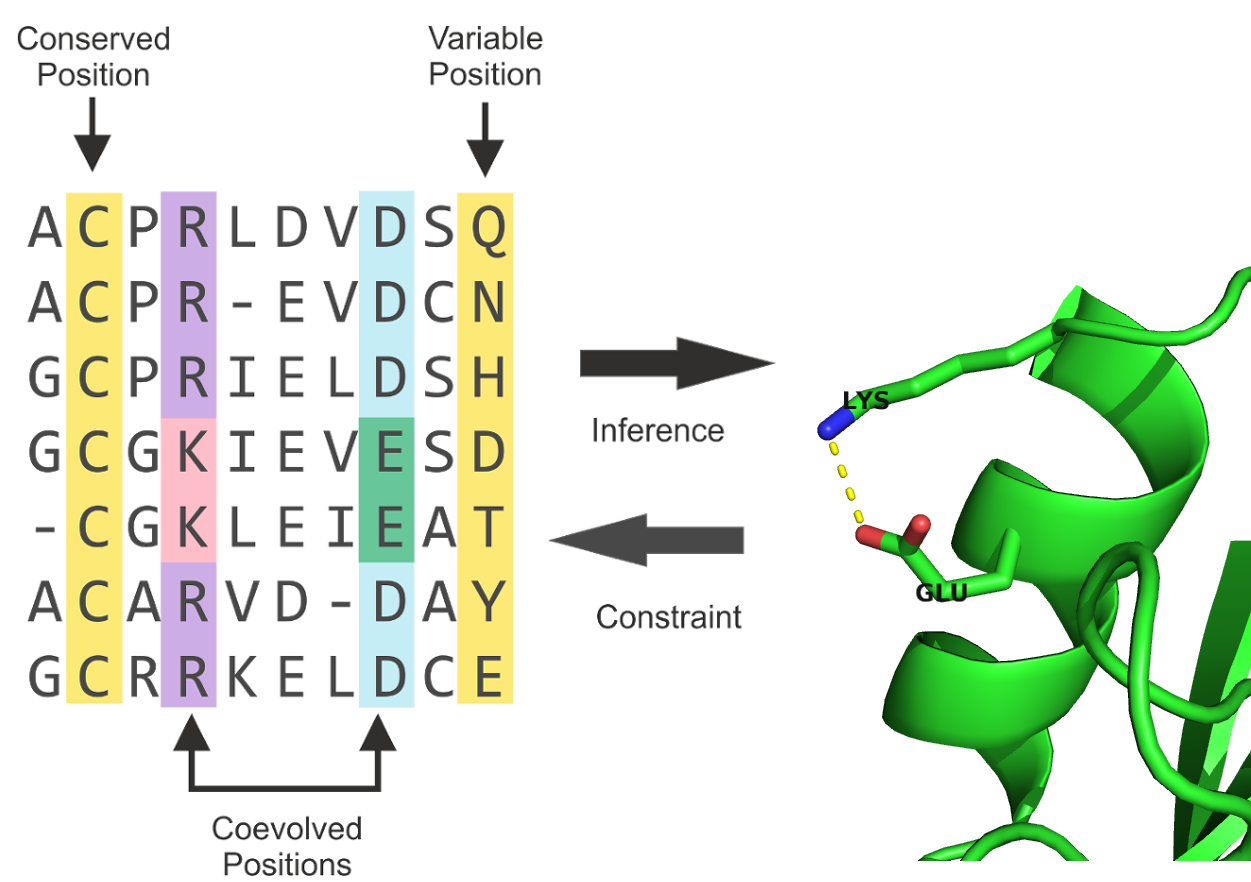
\includegraphics[width=0.9\linewidth]{img/intro/correlated-mutations-transparent} 

}

\caption{The evolutionary record of a protein
family reveals evidence of compensatory mutations between spatially
neighboring residues that are under selective pressure with respect to
some physico-chemical constraints. Mining protein family sequence
alignments for residue pairs with strong coevolutionary signals using
statistical methods allows inference of spatial proximity for these
residue pairs.}\label{fig:correlated-mutations}
\end{figure}

The following sections will give an overview over important methods and
developments in the field of contact prediction.

\section{Local Statistical Models}\label{local-methods}

Early contact prediction methods used local pairwise statistics to infer
contacts that regard pairs of amino acids in a sequence as statistically
independent from another.

Several of these methods use correlation coefficient based measures,
such as Pearson correlation between amino acid counts, properties
associated with amino acids or mutational propensities at the sites of a
\protect\hyperlink{abbrev}{MSA}
{[}\protect\hyperlink{ref-Gobel1994}{45},\protect\hyperlink{ref-Neher1994}{47}--\protect\hyperlink{ref-Shindyalov1994}{50}{]}.

Many methods have been developed that are rooted in information theory
and use \protect\hyperlink{abbrev}{MI} measures to describe the
dependencies between sites in the alignment
{[}\protect\hyperlink{ref-Clarke1995}{51}--\protect\hyperlink{ref-Martin2005}{53}{]}.
Phylogenetic and entropic biases have been identified as strong sources
of noise that confound the true coevolution signal
{[}\protect\hyperlink{ref-Martin2005}{53}--\protect\hyperlink{ref-Fodor2004}{55}{]}.
Different variants of \protect\hyperlink{abbrev}{MI} based approaches
address these effects and improve on the signal-to-noise ratio
{[}\protect\hyperlink{ref-Atchley2000}{54},\protect\hyperlink{ref-Tillier2003}{56},\protect\hyperlink{ref-Gouveia_Oliveira2007}{57}{]}.
The most prominent correction for background noises is
\protect\hyperlink{abbrev}{APC} that is still used by many modern
methods and is discussed in section \ref{post-processing-heuristics}
{[}\protect\hyperlink{ref-Dunn2008}{58}{]}. Another popular method is
\emph{OMES} that essentially computes a chi-squared statistic to detect
the differences between observed and expected pairwise amino acid
frequencies for a pair of columns
{[}\protect\hyperlink{ref-Kass2002}{59},\protect\hyperlink{ref-Noivirt2005}{60}{]}.

The traditional covariance approaches suffered from high false positive
rates because of their inability to cope with transitive effects that
arise from chains of correlations between multiple residue pairs
{[}\protect\hyperlink{ref-Lapedes1999}{61}--\protect\hyperlink{ref-Weigt2009}{63}{]}.
The concept of transitve effects is illustrated in Figure
\ref{fig:transitive-effect}. Considering three residues A, B and C,
where A physically interacts with B and B with C. Strong statistical
dependencies between pairs (A,B) and (B,C) can induce strong indirect
signals for residues A and C, eventhough they are not physically
interacting. These indirect correlations can become even larger than
signals of other directly interacting pairs (D,E) and thus lead to false
predictions {[}\protect\hyperlink{ref-Burger2010}{62}{]}.

Local statistical methods consider residue pairs independent of one
another which is why they cannot distinguish between direct and indirect
correlation signals. In contrast, global statistical models presented in
the next section learn a joint probability distribution over all
residues allowing to disentangle transitive effects
{[}\protect\hyperlink{ref-Burger2010}{62},\protect\hyperlink{ref-Weigt2009}{63}{]}.
Eventhough local statistical methods cannot compete with modern
predictors, \emph{OMES} and \protect\hyperlink{abbrev}{MI} based scores
often serve as a baseline in performance benchmarks for contact
prediction
{[}\protect\hyperlink{ref-DeJuan2013}{64},\protect\hyperlink{ref-Jones2012}{65}{]}.












\begin{figure}

{\centering 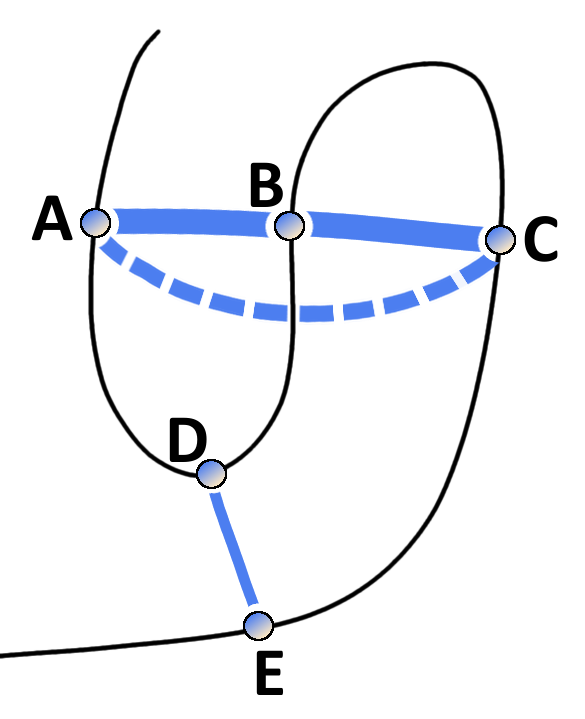
\includegraphics[width=0.25\linewidth]{img/intro/transitive_effects} 

}

\caption{Effects of chained covariation obscure
signals from true physical interactions. Consider residues A through E
with physical interactions between the residue pairs A-B, B-C and D-E.
The thickness of blue lines between residues reflects the strength of
statistical dependencies between the corresponding alignment columns.
Strong statistical dependencies between residue pairs (A,B) and (B,C)
can induce a strong dependency between the spatially distant residues A
and C. Covariation signals arising from transitive effects can become
even stronger than other direct covariation signals and lead to false
positive predictions.}\label{fig:transitive-effect}
\end{figure}

\section{Global Statistical Models}\label{global-methods}

A huge leap forward was the development of sophisticated statistical
models that make predictions for a single residue pair while considering
all other pairs in the protein. These global models allow for the
distinction between transitive and causal interactions which has been
referred to in the literature as \protect\hyperlink{abbrev}{DCA}
{[}\protect\hyperlink{ref-Lapedes1999}{61},\protect\hyperlink{ref-Weigt2009}{63}{]}.

In 1999 Lapedes et al. were the first to propose a global statistical
approach for the prediction of residue-residue contacts in order to
disentangle transitive effects
{[}\protect\hyperlink{ref-Lapedes1999}{61}{]}. They consider a Pott's
model that can be derived under a maximum entropy assumption and use the
model specific coupling parameters to infer interactions. At that time
the wider implications of this advancement went unnoted, but meanwhile
the Pott's Model has become the most prominent statistical model for
contact prediction. Section \ref{maxent} deals extensively with the
derivation and properties of the Pott's model, its application to
contact prediction and its numerous realizations.

A global statistical model not motivated by the maximum entropy approach
was proposed by Burger and Nijmwegen in 2010
{[}\protect\hyperlink{ref-Burger2010}{62},\protect\hyperlink{ref-Burger2008}{66}{]}.
Their fast Bayesian network model incorporates additional prior
information and phylogenetic correction via
\protect\hyperlink{abbrev}{APC} but cannot compete with the
pseudo-likelihood approaches presented in section
\ref{pseudo-likelihood}.

\section{Machine Learning Methods and
Meta-Predictors}\label{meta-predictors}

With the steady increase in protein sequence data, machine learning
based methods have emerged that extract features from
\protect\hyperlink{abbrev}{MSAs} in order to learn associations between
input features and residue-residue contacts. Sequence features typically
include predicted solvent accessibility, predicted secondary structure,
contact potentials, conservation scores, global protein features,
pairwise coevolution statistics and averages of certain features over
sequence windows. Numerous sequence-based methods have been developed
using machine learning algorithms, such as support support vector
machines (\emph{SVMCon} {[}\protect\hyperlink{ref-Cheng2007}{67}{]},
\emph{SVM-SEQ} {[}\protect\hyperlink{ref-Wu2008}{68}{]}), random forests
(\emph{ProC\_S3} {[}\protect\hyperlink{ref-Li2011}{69}{]}, \emph{TMhhcp}
{[}\protect\hyperlink{ref-Wang2011}{70}{]}, \emph{PhyCMap}
{[}\protect\hyperlink{ref-Wang2013}{71}{]}), neural networks
(\emph{NETCSS} {[}\protect\hyperlink{ref-Fariselli2001a}{72}{]},
\emph{SAM} {[}\protect\hyperlink{ref-Shackelford2007}{73}{]},
{[}\protect\hyperlink{ref-Hamilton2004a}{74}{]}, \emph{SPINE-2D}
{[}\protect\hyperlink{ref-Xue2009a}{75}{]}, \emph{NNCon}
{[}\protect\hyperlink{ref-Tegge2009a}{76}{]}) deep neural networks
(\emph{DNCon} {[}\protect\hyperlink{ref-Eickholt2012}{77}{]},
\emph{CMAPpro} {[}\protect\hyperlink{ref-DiLena2012a}{78}{]}) and
ensembles of genetic algorithm classfiers (\emph{GaC}
{[}\protect\hyperlink{ref-Chen2010}{79}{]}).

Different contact predictors, especially when rooted in distinct
principles like sequence-based and coevolution methods, provide
orthogonal information on the likelihood that a pair of residues makes a
contact
{[}\protect\hyperlink{ref-Cheng2007}{67},\protect\hyperlink{ref-Jones2015}{80}{]}.
The next logical step in method development therefore constitutes the
combination of several base predictors and classical sequence-derived
features in the form of meta-predictors.

The first published meta-predictor was \emph{PconsC} in 2013, combining
sequence features and predictions from the coevolution methods
\emph{PSICOV} and \emph{plmDCA}
{[}\protect\hyperlink{ref-Skwark2013}{81}{]}. In a follow-up version
\emph{PSICOV} has been replaced with \emph{gaussianDCA} and the
sequence-based method \emph{PhyCMap}
{[}\protect\hyperlink{ref-Skwark2016}{82}{]}. \emph{EPC-MAP} was
published in 2014 integrating \emph{GREMLIN} as a coevolution feature
with physicochemical information from predicted ab initio protein
structures {[}\protect\hyperlink{ref-Schneider2014}{83}{]}. In 2015,
\emph{MetaPSICOV} was released combining predictions from \emph{PSICOV},
\emph{mfDCA} and \emph{CCMpred} with other sequence derived feautures
{[}\protect\hyperlink{ref-Jones2015a}{84}{]}. \emph{RaptorX} uses
\emph{CCMpred} as coevolution feature and other standard contact
prediction features within an ultra-deep neural network
{[}\protect\hyperlink{ref-Wang2016a}{85}{]}. The newest developments
\emph{EPSILON-CP} and \emph{NeBcon} both comprise the most comprehensive
usage of contact prediction methods so far, combining five and eight
state-of-the-art contact predictors, respectively
{[}\protect\hyperlink{ref-Stahl2017}{86},\protect\hyperlink{ref-He2017}{87}{]}.

Another conceptual advancement besides the combination of sources of
information is based on the fact that contacts are not randomly or
independently distributed. DiLena and colleagues found that over 98\% of
long-range contacts (sequence separation \textgreater{} 24 positions)
are in close proximity of other contacts, compared to 30\% for
non-contacting pairs {[}\protect\hyperlink{ref-DiLena2012a}{78}{]}. The
distribution of contacts is governed by local structural elements, like
interactions between helices or \(\beta\)-sheets, leading to
characteristic patterns in the contact map that can be recognised
{[}\protect\hyperlink{ref-Andreani2015a}{88}{]}. Deep learning provides
the means to model higher level abstractions of data and several methods
apply multi-layered algorithms to refine predictions by learning
patterns that reflect the local neighborhood of a contact
{[}\protect\hyperlink{ref-DiLena2012a}{78},\protect\hyperlink{ref-Jones2015a}{84},\protect\hyperlink{ref-Wang2016a}{85},\protect\hyperlink{ref-Skwark2014a}{89}{]}.

Eventhough a benchmark comparing the recently developed meta-predictors
is yet to be made, it becomes clear from the recent
\protect\hyperlink{abbrev}{CASP} experiments, that meta-predictors
outperform pure coevolution methods
{[}\protect\hyperlink{ref-Monastyrskyy2015}{90}{]}. As coevolution
scores comprise the most informative feautures among the set of input
features, it is clear that meta-predictors will benefit from further
improvements of pure coevolution methods
{[}\protect\hyperlink{ref-Wang2016a}{85},\protect\hyperlink{ref-Stahl2017}{86}{]}.

\section{Modelling Protein Families with Potts Model}\label{maxent}

Infering contacts from a joint probability distribution over all
residues in a protein sequence instead of using simple pairwise
statistics has been proven to enable the distinction of direct
statistical dependencies between residues from indirect dependencies
mediated through other residues. The global statistical model that is
commonly used to describe this joint probability distribution is the
\emph{Potts model}. It is a well-established model in statistical
mechanics and can be derived from a maximum entropy assumption which is
explained in the following.

The principle of maximum entropy, proposed by Jaynes in 1957
{[}\protect\hyperlink{ref-Jaynes1957a}{91},\protect\hyperlink{ref-Jaynes1957b}{92}{]},
states that the probability distribution which makes minimal assumptions
and best represents observed data is the one that is in agreement with
measured constraints (prior information) and has the largest entropy. In
other words, from all distributions that are consistent with measured
data, the distribution with maximal entropy should be chosen.

A protein family is represented by a \protect\hyperlink{abbrev}{MSA}
\(\X = \{ \seq_1, \ldots, \seq_N \}\) of \(N\) protein sequences. Every
protein sequence of the protein family represents a sample drawn from a
target distribution \(p(\seq)\), so that each protein sequence is
associated with a probability. Each sequence
\(\seq_n = (\seq_{n1}, ..., \seq_{nL})\) is of length \(L\) and every
position constitutes a categorical variable \(x_{i}\) that can take
values from an alphabet indexed by \(\{0, ..., 20\}\), where 0 stands
for a gap and \(\{1, ... , 20\}\) stand for the 20 types of amino acids.
The measured constraints are given by the empirically observed single
and pairwise amino acid frequencies that can be calculated as

\begin{equation}
    f_i(a) = f(x_i\eq a) = \frac{1}{N}\sum_{n=1}^N I(x_{ni} \eq a) \; ,
\end{equation}

\begin{equation}
    f_{ij}(a,b) = f(x_i\eq a, x_j\eq b) = \frac{1}{N} \sum_{n=1}^N I(x_{ni} \eq a, x_{nj} \eq b) \; .
 \label{eq:emp-freq}
\end{equation}

According to the maximum entropy principle, the distribution \(p(\seq)\)
should have maximal entropy and reproduce the empirically observed amino
acid frequencies, so that

\begin{align}
   f(x_i\eq a)            &\equiv p(x_i\eq a)  \nonumber\\
                                    &= \sum_{\seq\prime_1, \ldots, \seq\prime_L = 1}^{q} p(x\prime) I(x\prime_i \eq a) \\
  f(x_i\eq a, x_j\eq b)   &\equiv p(x_i\eq a, x_j \eq b) \nonumber \\
                                    &= \sum_{\seq\prime_1, \ldots, \seq\prime_L = 1}^{q}  p(x\prime) I(x\prime_i\eq a, x\prime_j \eq b)  \; .
 \label{eq:maxent-reproducing-emp-freq}
\end{align}

Solving for the distribution \(p(\seq)\) that maximizes the Shannon
entropy \(S= -\sum_{\seq\prime} p(\seq\prime) \log p(\seq\prime)\) while
satisfying the constraints given by the empircial amino acid frequencies
in eq. \eqref{eq:maxent-reproducing-emp-freq} by introducing Lagrange
multipliers \(\wij\) and \(\vi\), results in the formulation of the
\emph{Potts model},

\begin{equation}
    p(\seq | \v, \w ) = \frac{1}{Z(\v, \w)} \exp \left( \sum_{i=1}^L v_i(x_i) \sum_{1 \leq i < j \leq L}^L w_{ij}(x_i, x_j) \right) \; .
\label{eq:max-ent-model}
\end{equation}

The Lagrange multipliers \(\wij\) and \(\vi\) remain as model parameters
to be fitted to data. \(Z\) is a normalization constant also known as
\emph{partition function} that ensures the total probabilty adds up to
one by summing over all possible assignments to \(\seq\),

\begin{equation}
  Z(\v, \w) = \sum_{\seq\prime_1, \ldots, \seq\prime_L = 1}^{q} \exp  \left( \sum_{i=1}^L v_i(x_i) \sum_{1 \leq i < j \leq L}^L w_{ij}(x_i, x_j) \right) \; .
  \label{eq:partition-fct-likelihood}
\end{equation}

\subsection{Model Properties}\label{potts-model-properties}

The Potts model is specified by singlet terms \(\via\) which describe
the tendency for each amino acid a to appear at position \(i\), and pair
terms \(\wijab\), also called couplings, which describe the tendency of
amino acid a at position \(i\) to co-occur with amino acid b at position
\(j\). In contrast to mere correlations, the couplings explain the
causative dependence structure between positions by jointly modelling
the distribution of all positions in a protein sequence and thus account
for transitive effects. By doing so, a major source of noise in contact
prediction methods is eliminated.

To get some intuition for the coupling coefficients, note that
\(\wijab = 1\) corresponds to a 2.7-fold higher probability for a and b
to occur together than what is expected from the singlet frequencies if
a and b were independent. Pairs of residues that are not in contact tend
to have negligable couplings, \(\wij \approx 0\), whereas pairs in
contact tend to have vectors significantly different from 0. For
contacting residues \(i\) and \(j\) in real world
\protect\hyperlink{abbrev}{MSAs} typical coupling strengths are on the
order of \(||\wij || \approx 0.1\) (regularization dependent).

Maximum entropy models naturally give rise to exponential family
distributions that express useful properties for statistical modelling,
such as the convexity of the likelihood function which consequently has
a unique, global minimum
{[}\protect\hyperlink{ref-Wainwright2007}{93},\protect\hyperlink{ref-Murphy2012}{94}{]}.

The Potts model is a discrete instance of what is referred to as a
pairwise \protect\hyperlink{abbrev}{Markov random field} in the
statistics community. \protect\hyperlink{abbrev}{MRFs} belong to the
class of undirected graphical models, that represent the probability
distribution in terms of a graph with nodes and edges characterizing the
variables and the dependence structure between variables, respectively.

\subsubsection{Gauge Invariance}\label{gauge-invariance}

As every variable \(x_{ni}\) can take \(q=21\) values, the model has
\(L \! \times \! q + L(L-1)/2 \! \times \! q^2\) parameters. But the
parameters are not uniquely determined and multiple parametrizations
yield identical probability distributions.

For example, adding a constant to all elements in \(v_i\) for any fixed
position \(i\) or similarly adding a constant to \(\via\) for any fixed
position \(i\) and amino acid \(a\) and subtracting the same constant
from the \(qL\) coefficients \(\wijab\) with \(b \in \{1, \ldots, q\}\)
and \(j \in \{1, \ldots, L \}\) leaves the probabilities for all
sequences under the model unchanged, since such a change will be
compensated by a change of \(Z(\v, \w)\) in eq.
\eqref{eq:partition-fct-likelihood}.

The overparametrization is referred to as \emph{gauge invariance} in
statistical physics literature and can be eliminated by removing
parameters
{[}\protect\hyperlink{ref-Weigt2009}{63},\protect\hyperlink{ref-Morcos2011}{95}{]}.
An appropriate choice of which parameters to remove, referred to as
\emph{gauge choice}, reduces the number of parameters to
\(L \! \times \! (q-1) + L(L-1)/2 \! \times \! (q-1)^2\). Popular gauge
choices are the \emph{zero-sum gauge} or \emph{Ising-gauge} used by
Weigt et al. {[}\protect\hyperlink{ref-Weigt2009}{63}{]} imposed by the
restraints,

\begin{equation}
    \sum_{a=1}^{q} v_{ia} = \sum_{a=1}^{q} \wijab = \sum_{a=1}^{q} w_{ijba} = 0
\label{eq:zero-sum-gauge}
\end{equation}

for all \(i,j,b\) or the \emph{lattice-gas gauge} used by Morcos et al
{[}\protect\hyperlink{ref-Morcos2011}{95}{]} and Marks et al
{[}\protect\hyperlink{ref-Marks2011}{38}{]} imposed by restraints

\begin{equation}
    \wij(q,a) = \wij(a,q) = \vi(q) = 0
\label{eq:ising-gauge}
\end{equation}

for all \(i,j,a\) {[}\protect\hyperlink{ref-Cocco2017}{96}{]}.

Alternatively, the indeterminacy can be fixed by including a
regularization prior (see next section). The regularizer selects for a
unique solution among all parametrizations of the optimal distribution
and therefore eliminates the need to choose a gauge
{[}\protect\hyperlink{ref-Koller2009}{97}--\protect\hyperlink{ref-Stein2015a}{99}{]}.

\subsection{Inferring Parameters for the Potts Model}\label{potts-mle}

Typically, parameter estimates are obtained by maximizing the
log-likelihood function of the parameters over observed data. For the
Potts model, the log-likelihood function is computed over sequences in
the alignment \(\mathbf{X}\):

\begin{align}
    \text{LL}(\v, \w | \mathbf{X}) =& \sum_{n=1}^N \log p(\seq_n)  \nonumber\\
    =& \sum_{n=1}^N \left[ \sum_{i=1}^L v_i(x_{ni}) + \sum_{1 \leq i < j \leq L}^L w_{ij}(x_{xn}, x_{nj}) - \log Z \right]
\label{eq:full-log-likelihood}
\end{align}

The number of parameters in a Potts model is typically larger than the
number of observations, i.e.~the number of sequences in the
\protect\hyperlink{abbrev}{MSA}. Considering a protein of length
\(L=100\), there are approximately \(2 \times 10^6\) parameters in the
model whereas the largest protein families comprise only around \(10^5\)
sequences (see Figure \ref{fig:pfam}). An underdetermined problem like
this renders the use of regularizers neccessary in order to prevent
overfitting.

Typically, an L2-regularization is used that pushes the single and
pairwise terms smoothly towards zero and is equivalent to the logarithm
of a zero-centered Gaussian prior,

\begin{align}
  R(\v, \w)  &= \log \left[ \mathcal{N}(\v | \mathbf{0}, \lambda_v^{-1} I) \mathcal{N}(\w | \mathbf{0}, \lambda_w^{-1} I) \right] \nonumber \\
             &= -\frac{\lambda_v}{2} ||\v||_2^2 - \frac{\lambda_w}{2} ||\w||_2^2 + \text{const.} \; ,
\label{eq:l2-reg}
\end{align}

where the strength of regularization is tuned via the regularization
coefficients \(\lambda_v\) and \(\lambda_w\)
{[}\protect\hyperlink{ref-Seemayer2014}{100}--\protect\hyperlink{ref-Kamisetty2013}{102}{]}.

However, optimizing the log-likelihood requires computing the partition
function \(Z\) given in eq. \eqref{eq:partition-fct-likelihood} that sums
\(q^L\) terms. Computing this sum is intractable for realistic protein
domains with more than 100 residues. Consequently, evaluating the
likelihood function at each iteration of an optimization procedure is
infeasible due to the exponential complexity of the partition function
in protein length \(L\).

Many approximate inference techniques have been developed to sidestep
the infeasible computation of the partition function for the specific
problem of predicting contacts that are briefly explained in the next
section.

\subsection{Solving the Inverse Potts
Problem}\label{potts-model-solutions}

In 1999 Lapedes et al. were the first to propose maximum entropy models
for the prediction of residue-residue contacts in order to disentangle
transitive effects {[}\protect\hyperlink{ref-Lapedes1999}{61}{]}. In
2002 they applied their idea to 11 small proteins using an iterative
Monte Carlo procedure to obtain estimates of the model parameters and
achieved an increase in accuracy of 10-20\% compared to the local
statistical models {[}\protect\hyperlink{ref-Lapedes2012a}{103}{]}. As
the calculations involved were very time-consuming and at that time
required supercomputing resources, the wider implications were not noted
yet.

Ten years later Weight et al proposed an iterative message-passing
algorithm, here referred to as \emph{mpDCA}, to approximate the
partition function {[}\protect\hyperlink{ref-Weigt2009}{63}{]}.
Eventhough their approach is computationally very expensive and in
practice only applicable to small proteins, they obtained remarkable
results for the two-component signaling system in bacteria.

Balakrishnan et al were the first to apply pseudo-likelihood
approximations to the full likelihood in 2011
{[}\protect\hyperlink{ref-Balakrishnan2011}{104}{]}. The
pseudo-likelihood optimizes a different objective and replaces the
global partition function \(Z\) with local estimates. Balakrishnan and
colleagues applied their method \emph{GREMLIN} to learn sparse graphical
models for 71 protein families. In a follow-up study in 2013, the
authors proposed an improved version of \emph{GREMLIN} that uses
additional prior information
{[}\protect\hyperlink{ref-Kamisetty2013}{102}{]}.

Also in 2011, Morcos et al. introduced a naive mean-field inversion
approximation to the partition function, named \emph{mfDCA}
{[}\protect\hyperlink{ref-Morcos2011}{95}{]}. This method allows for
drastically shorter running times as the mean-field approach boils down
to inverting the empirical covariance matrix calculated from observed
amino acid frequencies for each residue pair \(i\) and \(j\) of the
alignment. This study performed the first high-throughput analysis of
intradomain contacts for 131 protein families and facilitated the
prediction of protein structures from accurately predicted contacts in
{[}\protect\hyperlink{ref-Marks2011}{38}{]}.

The initial work by Balakrishnan and collegueas went almost unnoted as
it was not primarily targeted to the problem of contact prediction.
Ekeberg and collegueas independently developed the pseudo-likelihood
method \emph{plmDCA} in 2013 and showed its superior precision over
\emph{mfDCA} {[}\protect\hyperlink{ref-Ekeberg2013}{98}{]}.

A related approach to mean-field approximation is sparse inverse
covariance estimation, named \emph{PSICOV}, developed by Jones et al.
(2012) {[}\protect\hyperlink{ref-Jones2012}{65}{]}. PSICOV uses an
L1-regularization, known as graphical Lasso, to invert the correlation
matrix and learn a sparse graphical model
{[}\protect\hyperlink{ref-Friedman2008}{105}{]}. Both procedures,
\emph{mfDCA} and \emph{PSICOV}, assume the model distribution to be a
multivariate Gaussian. It has been shown by Banerjee et al. (2008)that
this dual optimization solution also applies to binary data, as is the
case in this application, where each position is encoded as a
20-dimensional binary vector
{[}\protect\hyperlink{ref-Banerjee2008}{106}{]}.

Another related approach to \emph{mfDCA} and \emph{PSICOV} is
\emph{gaussianDCA}, proposed in 2014 by Baldassi et al.
{[}\protect\hyperlink{ref-Baldassi2014}{107}{]}. Similar to the other
both approaches, they model the data as multivariate Gaussian but within
a simple Bayesian formalism by using a suitable prior and estimating
parameters over the posterior distribution.

So far, pseudo-likelihood has proven to be the most successful
approximation of the likelihood with respect to contact prediction
performance. Currently, there exist several implementations of
pseudo-likelihood maximization that vary in slight details, perform
similarly and thus are equally popular in the community, such as CCMpred
{[}\protect\hyperlink{ref-Seemayer2014}{100}{]},
plmDCA{[}\protect\hyperlink{ref-Ekeberg2014}{101}{]} and GREMLIN
{[}\protect\hyperlink{ref-Kamisetty2013}{102}{]}.

\subsubsection{Maximum Likelihood Inference for
Pseudo-Likelihood}\label{pseudo-likelihood}

The pseudo-likelihood is a rather old estimation principle that was
suggested by Besag already in 1975
{[}\protect\hyperlink{ref-Besag1975}{108}{]}. It represents a different
objective function than the full likelihood and approximates the joint
probability with the product over conditionals for each variable,
i.e.~the conditional probability of observing one variable given all the
others:

\begin{align}
  p(\seq | \v,\w) \approx&   \prod_{i=1}^L p(x_i | \seq_{\backslash xi}, \v,\w) \nonumber \\
                        =&  \prod_{i=1}^L \frac{1}{Z_i} \exp \left(  v_i(x_i) \sum_{1 \leq i < j \leq L}^L w_{ij}(x_i, x_j) \right)
\end{align}

Here, the normalization term \(Z_i\) sums only over all assignments to
one position \(i\) in sequence:

\begin{equation}
  Z_i = \sum_{a=1}^{q} \exp \left( v_i(a) \sum_{1 \leq i < j \leq L}^L w_{ij}(a, x_j) \right)
\label{eq:partition-fct-pll}
\end{equation}

Replacing the global partition function in the full likelihood with
local estimates of lower complexity in the pseudo-likelihood objective
resolves the computational intractability of the parameter optimization
procedure. Hence, it is feasible to maximize the pseudo-log-likelihood
function,

\begin{align}
    \text{pLL}(\v, \w | \mathbf{X}) =& \sum_{n=1}^N \sum_{i=1}^L \log p(x_i | \seq_{\backslash xi}, \v,\w) \nonumber \\
    =& \sum_{n=1}^N \sum_{i=1}^L  \left[ v_i(x_{ni}) + \sum_{j=i+1}^L  w_{ij}(x_{ni}, x_{nj}) - \log Z_{ni} \right] \;,
\end{align}

plus an additional regularization term in order to prevent overfitting
and to fix the gauge to arrive at a \protect\hyperlink{abbrev}{MAP}
estimate of the parameters,

\begin{equation}
    \hat{\v}, \hat{\w} = \underset{\v, \w}{\operatorname{argmax}} \; \text{pLL}(\v, \w | \mathbf{X}) + R(\v, \w) \; .
\end{equation}

Eventhough the pseudo-likelihood optimizes a different objective than
the full-likelihood, it has been found to work well in practice for many
problems, including contact prediction
{[}\protect\hyperlink{ref-Murphy2012}{94},\protect\hyperlink{ref-Koller2009}{97}--\protect\hyperlink{ref-Stein2015a}{99}{]}.
The pseudo-likelihood function retains the concavity of the likelihood
and it has been proven to be a consistent estimator in the limit of
infinite data for models of the exponential family
{[}\protect\hyperlink{ref-Koller2009}{97},\protect\hyperlink{ref-Besag1975}{108},\protect\hyperlink{ref-Gidas1988}{109}{]}.
That is, as the number of sequences in the alignment increases,
pseudo-likelihood estimates converge towards the true full likelihood
parameters.

\subsection{Computing Contact Maps}\label{post-processing-heuristics}

Model inference as described in the last section yields
\protect\hyperlink{abbrev}{MAP} estimates of the couplings
\(\hat{\w}_{ij}\). In order to obtain a scalar measure for the coupling
strength between two residues \(i\) and \(j\), all available methods
presented in section \ref{potts-model-solutions} heuristically map the
\(21 \! \times \! 21\) dimensional coupling matrix \(\wij\) to a single
scalar quantity.

\emph{mpDCA} {[}\protect\hyperlink{ref-Weigt2009}{63}{]} and
\emph{mfDCA}
{[}\protect\hyperlink{ref-Marks2011}{38},\protect\hyperlink{ref-Morcos2011}{95}{]}
employ a score called \protect\hyperlink{abbrev}{DI}, that essentially
computes the \protect\hyperlink{abbrev}{MI} for two positions \(i\) and
\(j\) using the couplings \(\wij\) instead of pairwise amino acid
frequencies. Most pseudo-likelihood methods (\emph{plmDCA}
{[}\protect\hyperlink{ref-Ekeberg2013}{98},\protect\hyperlink{ref-Ekeberg2014}{101}{]},
\emph{CCMpred} {[}\protect\hyperlink{ref-Seemayer2014}{100}{]},
\emph{GREMLIN} {[}\protect\hyperlink{ref-Kamisetty2013}{102}{]}) compute
the \emph{Frobenius norm} of the coupling matrix \(\wij\) to obtain a
scalar contact score \(C_{ij}\),

\begin{equation}
    C_{ij}  = ||\wij||_2 = \sqrt{\sum_{a,b=1}^q \wijab^2} \; .
\label{eq:frobenius-norm}
\end{equation}

The Frobenius norm improves prediction performance over
\protect\hyperlink{abbrev}{DI} and further improvements can be obtained
by computing the Frobenius norm only on the \(20 \times 20\) submatrix
thus ignoring contributions from gaps
{[}\protect\hyperlink{ref-Ekeberg2013}{98},\protect\hyperlink{ref-Baldassi2014}{107},\protect\hyperlink{ref-Feinauer2014}{110}{]}.
\emph{PSICOV} {[}\protect\hyperlink{ref-Jones2012}{65}{]} uses an
L1-norm on the \(20 \times 20\) submatrix instead of the Frobenius norm.

Furthermore it should be noted that the Frobenius norm is gauge
dependent and is minimized by the \emph{zero-sum gauge}
{[}\protect\hyperlink{ref-Weigt2009}{63}{]}. Therefore, the coupling
matrices should be transformed to \emph{zero-sum gauge} before computing
the Frobenius norm

\begin{equation}
    \w^{\prime}_{ij}  = \wij - \wij(\cdot, b) - \wij(a, \cdot) + \wij(\cdot, \cdot) \; ,
\label{eq:zero-sum-gauge-transform}
\end{equation}

where \(\cdot\) denotes average over the respective indices
{[}\protect\hyperlink{ref-Ekeberg2013}{98},\protect\hyperlink{ref-Seemayer2014}{100},\protect\hyperlink{ref-Ekeberg2014}{101},\protect\hyperlink{ref-Baldassi2014}{107}{]}.

Another commonly applied heuristic known as
\protect\hyperlink{abbrev}{APC} has been introduced by Dunn et al. in
order to reduce background noise arising from correlations between
positions with high entropy or phylogenetic couplings
{[}\protect\hyperlink{ref-Dunn2008}{58}{]}.
\protect\hyperlink{abbrev}{APC} is a correction term that is computed
from the raw contact map as the product over average row and column
contact scores \(\overline{C_i}\) divided by the average contact score
over all pairs \(\overline{C_{ij}}\). The corrected contact score
\(C_{ij}^{APC}\) is obtained by subtracting the
\protect\hyperlink{abbrev}{APC} term from the raw contact score
\(C_{ij}\),

\begin{equation}
    C_{ij}^{APC}  = C_{ij} - \frac{\overline{C_i} \; \overline{C_j}}{\overline{C_{ij}}}\; .
\label{eq:apc}
\end{equation}

Visually, \protect\hyperlink{abbrev}{APC} creates a \emph{smoothing}
effect on the contact maps that is illustrated in Figure
\ref{fig:apc-correction} and it has been found to substantially boost
contact prediction performance
{[}\protect\hyperlink{ref-Dunn2008}{58},\protect\hyperlink{ref-Kamisetty2013}{102}{]}.
It was first adopted by \emph{PSICOV}
{[}\protect\hyperlink{ref-Jones2012}{65}{]} but is now used by most
methods to adjust raw contact scores.

It was long under debate why \protect\hyperlink{abbrev}{APC} works so
well and how it can be interpreted. Zhang et al. showed that
\protect\hyperlink{abbrev}{APC} essentially approximates the first
principal component of the contact matrix and therefore removes the
highest variability in the matrix that is assumed to arise from
background biases {[}\protect\hyperlink{ref-Zhang2016}{111}{]}.
Furthermore, they studied an advanced decomposition technique, called
LRS matrix decomposition, that decomposes the contact matrix into a
low-rank and a sparse component, representing background noise and true
correlations, respectively.\\
Inferring contacts from the sparse component works astonishing well,
improving precision further over \protect\hyperlink{abbrev}{APC}
independent of the underlying statistical model.

Dr Stefan Seemayer could show that the main component of background
noise can be attributed to entropic effects and that a substantial part
of \protect\hyperlink{abbrev}{APC} amounts to correcting for these
entropic biases (unpublished). In his doctoral thesis, he developed an
entropy correction, computed as the geometric mean of per-column
entropies, that correlates well with the \protect\hyperlink{abbrev}{APC}
correction term and yields similar precision for predicted contacts. The
entropy correction has the advantage that it is computed from input
statistics and therefore is independent of the statistical model used to
infer the couplings. In contrast, \protect\hyperlink{abbrev}{APC} and
other denoising techniques such as LRS
{[}\protect\hyperlink{ref-Zhang2016}{111}{]} discussed above, estimate a
background model from the final contact matrix, thus depending on the
statistical model used to infer the contact matrix.















\begin{figure}

{\centering 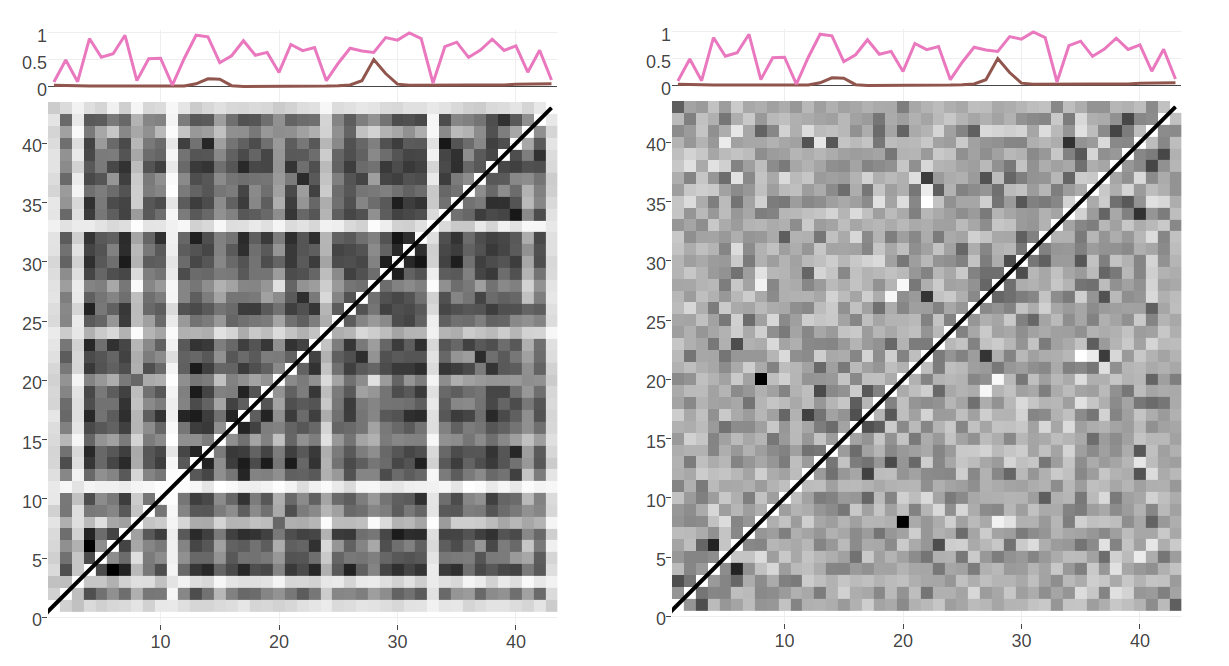
\includegraphics[width=0.9\linewidth]{img/intro/apc_correction_with_entropy} 

}

\caption{Contact maps computed from
pseudo-likelihood couplings. Subplot on top of the contact maps
illustrates the normalized Shannon entropy ({pink } line) and percentage
of gaps for every position in the alignment ({brown } line).
\textbf{Left}: Contact map computed with Frobenius norm as in eq.
\eqref{eq:frobenius-norm}. Overall coupling values are dominated by
entropic effects, i.e.~the amount of variation for a
\protect\hyperlink{abbrev}{MSA} position, leading to striped brightness
patterns. For example, positions with high column entropy
(e.g.~positions 7, 12 or 31) have higher overall coupling values than
positions with low column entropy (e.g.~positions 11, 24 or 33).
\textbf{b}: previous contact map but corrected for background noise with
the \protect\hyperlink{abbrev}{APC} as in eq. \eqref{eq:apc}.}\label{fig:apc-correction}
\end{figure}

\section{Applications}\label{application-contact-prediction}

The most popular and historically motivated application for contact
prediction is contact-guided \emph{de novo} structure prediction.

It has long been known that the native protein 3D structure can be
reconstructed from an error-free contact map
{[}\protect\hyperlink{ref-Vendruscolo1997}{39}{]}. Also, protein fold
reconstruction from sparse inter-residue proximity constraints obtained
from experiments such as cross-linking/mass spectrometry, Foerster
resonance energy transfer (FRET) or sparse nuclear Overhauser
enhancement (NOE) distance data generated from NMR experiments has been
demonstrated
{[}\protect\hyperlink{ref-Li2004}{32},\protect\hyperlink{ref-Yu2013}{112}--\protect\hyperlink{ref-Aszodi1995a}{116}{]}.
Predicted contacts, however, have long been regarded as being of little
use for structure prediction because of their high false-positive rates
{[}\protect\hyperlink{ref-Wu2011}{117},\protect\hyperlink{ref-Tress2010}{118}{]}.
Only with the emergence of global statistical models for contact
prediction which drastically reduced false-positive rates there has been
renewed interest in \emph{de novo} structure prediction aided by
predicted contacts. In 2011, Marks et al. showed that the top scoring
contacts predicted with their mean-field approach \emph{mfDCA} are
sufficiently accurate to successfully deduce the native fold of the
protein {[}\protect\hyperlink{ref-Marks2011}{38}{]}. In the following
years, methods to predict contacts have been improved and applied to
model many more protein structures culminating in the high-throughput
prediction of 614 protein structures out of which more than 100
represent novel folds by Ovchinnikov and colleagues in 2017
{[}\protect\hyperlink{ref-Hopf2012}{119}--\protect\hyperlink{ref-Ovchinnikov2017}{127}{]}.

Many contact-guided protocols have been established since, that
typically integrate predicted contacts in form of distance constraints
into an energy function to guide the conformational sampling process:
Unicon3D {[}\protect\hyperlink{ref-Bhattacharya2016}{128}{]}, RASREC
{[}\protect\hyperlink{ref-Braun2015}{129}{]}, RBOAleph
{[}\protect\hyperlink{ref-Mabrouk2015a}{130}{]}, GDFuzz3D
{[}\protect\hyperlink{ref-Pietal2015a}{131}{]}, PconsFold
{[}\protect\hyperlink{ref-Michel2014}{132}{]}, C2S\_Pipeline
{[}\protect\hyperlink{ref-Konopka2014}{133}{]}, FRAGFOLD + PSICOV
{[}\protect\hyperlink{ref-Kosciolek2014}{134}{]}, FILM3
{[}\protect\hyperlink{ref-Nugent2012}{135}{]}, EVFold
{[}\protect\hyperlink{ref-Marks2011}{38}{]}. Figure
\ref{fig:contact-assisted-structure-prediction} presents a generalized
structure prediction pipeline using predicted contacts.





\begin{figure}

{\centering 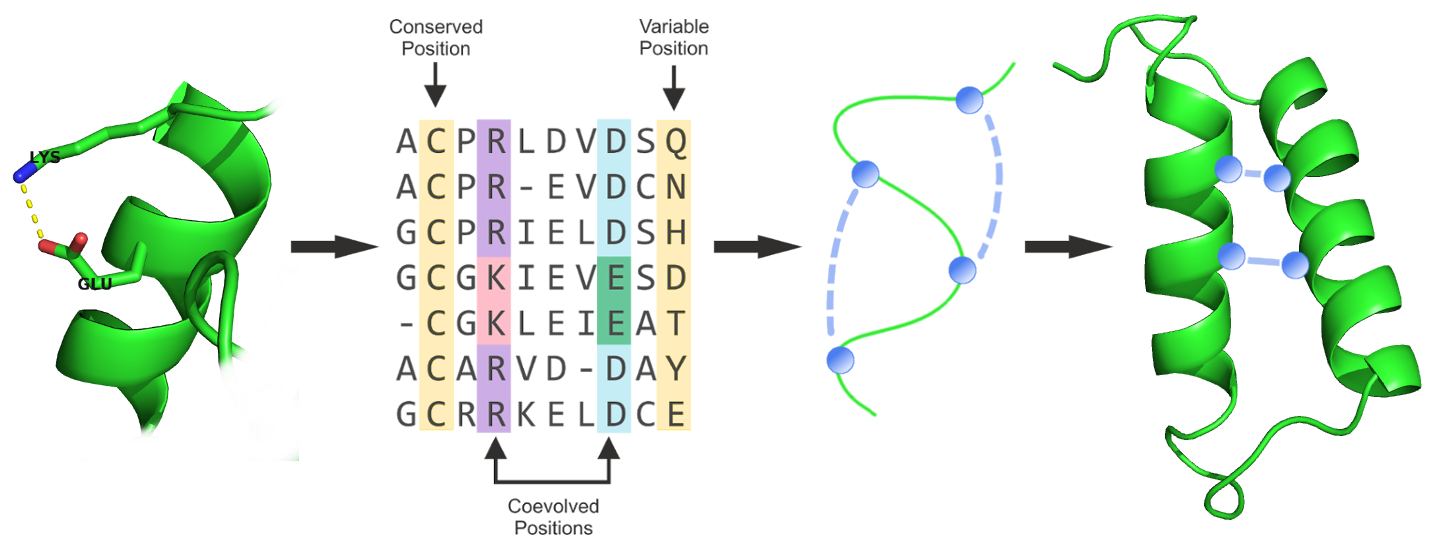
\includegraphics[width=1\linewidth]{img/intro/contact_assisted_structure_prediction} 

}

\caption{Generalized
structure prediction pipeline integrating predicted contacts in form of
distance constraints that guide conformational sampling.}\label{fig:contact-assisted-structure-prediction}
\end{figure}

The optimal quality of inferred contacts and their effective utilization
is still subject to discussion and further research. It has been
demonstrated that only a small subset of native contacts is sufficient
to produce accurate structural models
{[}\protect\hyperlink{ref-Vendruscolo1997}{39},\protect\hyperlink{ref-Kim2014}{40},\protect\hyperlink{ref-Konopka2014}{133},\protect\hyperlink{ref-Sathyapriya2009}{136}--\protect\hyperlink{ref-Vassura2007}{138}{]}.
Sathyapriya and colleagues developed a rational strategy to select
important native contacts and successfully reconstructed the structure
to near native resolution with only 8\% of contacts
{[}\protect\hyperlink{ref-Sathyapriya2009}{136}{]}. Kim and colleagues
formulated that only one correct contact for every 12 residues in the
protein is sufficient to allow accurate topology level modeling given
that the contacts are nonlocal and broadly distributed
{[}\protect\hyperlink{ref-Kim2014}{40}{]}. These studies emphasize that
certain contacts are more important than others. Long-range contacts are
rare and most informative for protein structure prediction because they
define the overal fold and packing of tertiary structure whereas
short-range contacts define local secondary structure
{[}\protect\hyperlink{ref-Adhikari2017}{139}{]}. It is a consistent
finding that eventhough long-range contacts are of higher relevance than
short-range contacts for structure reconstruction, their information
alone is not sufficient
{[}\protect\hyperlink{ref-Kosciolek2014}{134},\protect\hyperlink{ref-Sathyapriya2009}{136},\protect\hyperlink{ref-DiLena2009a}{140}{]}.
Since a small number of correct residue-residue contacts is sufficient
to improve protein structure prediction and many reconstruction
protocols can tolerate missing contact information much better than
erroneous contact information, it has been stressed that methods
development should focus on predicting a small number of high confident
contacts
{[}\protect\hyperlink{ref-Kim2014}{40},\protect\hyperlink{ref-Duarte2010}{41}{]}.
Marks and colleagues observed that isolated false positives have a much
stronger detrimental effect on structure prediction than false positives
close to true contacts {[}\protect\hyperlink{ref-Marks2011}{38}{]}.
Zhang et al. found that their tool Touchstone II required an accuracy of
long-range contact predictions of at least 22\% to generate a positive
effect to structure prediction
{[}\protect\hyperlink{ref-Zhang2003}{141}{]}. Frequently, folding
protocols employ a filtering step to eliminate unsatisfied or
conflicting constraints possibly originating from false-positive
contacts
{[}\protect\hyperlink{ref-Wang2016}{142},\protect\hyperlink{ref-Adhikari2015a}{143}{]}.
Generally it is assumed that higher precision of predicted long-range
contacts results in improved structural models, albeit there is no
strong correlation as model quality depends on many other factors such
as the secondary structure composition of the protein, the domain size,
the usage of additional sources of structural information, the type of
distance constraint function and the particular structure reconstruction
protocol
{[}\protect\hyperlink{ref-Marks2011}{38},\protect\hyperlink{ref-Kosciolek2014}{134},\protect\hyperlink{ref-Adhikari2017}{139},\protect\hyperlink{ref-Zhang2003}{141},\protect\hyperlink{ref-DeOliveira2016}{144}{]}.

Coevolution has not only been studied for residues pairs within a
protein but also for residue pairs across protein--protein interfaces
{[}\protect\hyperlink{ref-Ovchinnikov2014a}{120},\protect\hyperlink{ref-Hopf2014}{121},\protect\hyperlink{ref-Ovchinnikov2015a}{126},\protect\hyperlink{ref-Rodriguez-Rivas2016}{145},\protect\hyperlink{ref-Feinauer2016a}{146}{]}.
Eventhough the methodology of detecting coevolving amino acid pairs from
the \protect\hyperlink{abbrev}{MSA} is the same, a new challenge arises
for the correct identification of orthologous interacting partners.
Without the correct pairing of interacting partners for every species
the detection of coevolutionary signals would be compromised. However,
the generation of a \protect\hyperlink{abbrev}{MSA} of paired sequences
is complicated in the presence of multiple paralogs of a gene in a
single genome. The problem of paralog matching is visualized in Figure
\ref{fig:matching-sequences-ppi}. For prokaryotes, sequence paires are
typically identified by exploiting the bacterial gene organisation in
form of operons, i.e.~co-localized genes will be co-expressed and are
more likely to physically interact. Co-localisation of genes has also
been applied to match genes from eurkaryotes, assuming that Uniprot
accession numbers can be used as a proxy for genomic distances
{[}\protect\hyperlink{ref-Feinauer2016a}{146}{]}. New strategies have
been developed based on the idea that an alignment with correctly
matched paralogs will maximize the coevolution score
{[}\protect\hyperlink{ref-Gueudre2016}{147},\protect\hyperlink{ref-Bitbol2016}{148}{]}.







\begin{figure}

{\centering 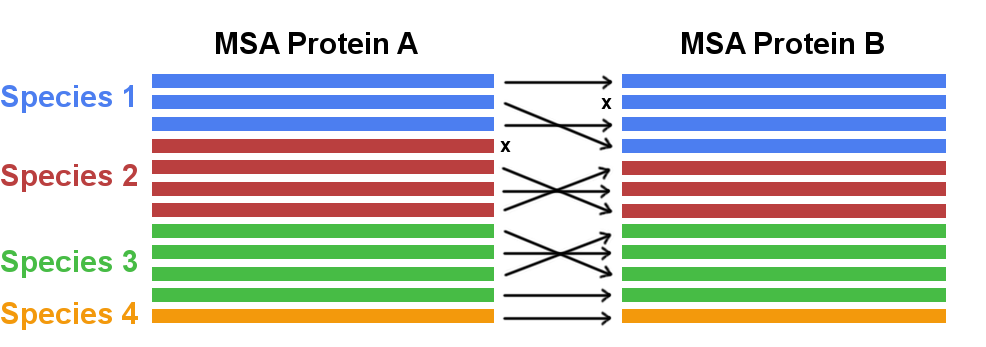
\includegraphics[width=1\linewidth]{img/intro/matching_sequences_ppi} 

}

\caption{Concatenating two multiple sequence
alignments. In case multiple paralogs exist for a gene in one species
the correct interaction partner needs to be identified and matched
(marked with arrows). Sequences that cannot be paired with a unique
interaction partner need to be discarded (marked with x).}\label{fig:matching-sequences-ppi}
\end{figure}

A related objective is the study of the oligomerization status of
proteins. The study of homo-oligomers is simplified in the sense that
the identical protein sequence of both interaction partners renders the
concatenation of two \protect\hyperlink{abbrev}{MSAs} unnessary and
allows to work with one \protect\hyperlink{abbrev}{MSA}. A different
challenge lies in the correct distinction between the physical contacts
of the monomeric structure and the interprotein contacts. With the
availability of monomeric structural data the idea is to filter out
those high scoring contacts that form contacts in the monomeric
structure or are located in the protein core. The remaining high scoring
false positive contacts at the surface of the protein are potential
contacts at the interface that can be incorporated into a docking
protocol to drive complex formation
{[}\protect\hyperlink{ref-Uguzzoni2017}{149},\protect\hyperlink{ref-DosSantos2015a}{150}{]}.

Contacts are also used to analyse potential alternative conformations of
proteins
{[}\protect\hyperlink{ref-Parisi2015a}{43},\protect\hyperlink{ref-Sfriso2016}{151}--\protect\hyperlink{ref-Jeon2011a}{155}{]}.
Coevolutionary analysis detects all evolutionarily significant
residue--residue correlations, regardless of whether the interaction is
formed in a transient state of the protein or its stable form.
Therefore, predicted contact maps might capture multiple states of a
protein, since they are of functional importance and thus under
evolutionary pressure. Sfriso and colleagues developed an automated
pipiline that introduces filtered predicted contacts as ensemble
restraints into a molecular dynamics simulations and is able to detect
alternative relevant conformational states
{[}\protect\hyperlink{ref-Sfriso2016}{151}{]}.

Quality assessment of structural models, involving model selection and
ranking, is a crucial task in structural biology. Predicted
residue-residue contacts can indicate the best protein structure among a
set of properly folded and misfolded structures by counting the number
of satisfied contacts
{[}\protect\hyperlink{ref-Tress2010}{118},\protect\hyperlink{ref-Wozniak2017}{156}{]}.
Besides ranking of models, predicted contacts have been used as features
for training machine learning methods that predict the global quality of
a structural model
{[}\protect\hyperlink{ref-Cao2016}{157},\protect\hyperlink{ref-Terashi2014a}{158}{]}.

As mentioned before, methods for protein fold reconstruction from
experimental distance constraints have been successfully applied for
many years. Several integrative approaches have been developed that
combine complementary sources of sparse structural constraints,
including predicted contacts, to accurately determine protein structure
{[}\protect\hyperlink{ref-Ward2013}{36},\protect\hyperlink{ref-Tang2015}{37}{]}.

Sadowski used predicted contacts to parse domain boundaries based on the
simple idea that contacts are more abundant within domains than between
domains {[}\protect\hyperlink{ref-Sadowski2013}{42}{]}.

Eventhough the coevolutionary methods have been developed for proteins,
they have been successfully applied to analyse nucleotide coevolution
and to predict RNA tertiary structures with the help of predicted
nucleotide-nucleotide contacts
{[}\protect\hyperlink{ref-Nawy2016}{159}--\protect\hyperlink{ref-DeLeonardis2015a}{161}{]}.
Much less RNA sequences are required compared to protein sequences in
order to extract statistically significant signals because of the
reduced number of model parameters when working with a four letter
alphabet (compared to a 20 letter alphabet with proteins). On the
downside, alignment errors resulting from the complicated determination
of RNA multiple sequence alignments limits the accuracy of coevolution
analysis {[}\protect\hyperlink{ref-DeLeonardis2015a}{161}{]}. Despite
the diminished accuracy, predicted nucleotide contacts have been
demonstrated to improve RNA structure prediction over conventional
methods {[}\protect\hyperlink{ref-Weinreb2015}{160}{]}.

The stastistical models used for coevolution analysis provide
information about which residue pairs are important in evolution for
folding or functional constraints. They can be used to assign
probabilities to sequences that reflect the overal compliance of a
sequence with the protein family under study and thereby provide
quantitative predictions of mutational effects
{[}\protect\hyperlink{ref-Hopf2017}{44},\protect\hyperlink{ref-Wu2016}{162},\protect\hyperlink{ref-Figliuzzi2015}{163}{]}.
Computational screening of mutational effects can support and complement
the costly and time-consuming directed evolution or mutational screening
experiments {[}\protect\hyperlink{ref-Hopf2017}{44}{]}. With a similar
idea in mind, the coevolution models have been applied to sequences of
human immune repertoires
{[}\protect\hyperlink{ref-Asti2016}{164},\protect\hyperlink{ref-Elhanati2014}{165}{]}.
Antibody affinity maturation can be viewed as a Darwinian process with
the affinity to the target antigen being the main fitness criterion.
Therefore, given the model representing the antibody sequence family,
the probability for a sequence reflects the binding affinity to the
target antigen. Quantifying the effect of mutations is also helpful for
protein design. Coevolving positions might be of particular interest as
hotspots for engineering protein stability or functional specificity
because they determine positions relevant to protein structure and
function {[}\protect\hyperlink{ref-Franceus2016}{166}{]}.

Skwark and colleagues applied the popular coevolution statistical models
to genomes and developed a statistical method called \emph{genomeDCA}
{[}\protect\hyperlink{ref-Skwark2017}{167}{]}. They are able to identify
coevolving polymorphic locus pairs based on the idea that the
corresponding proteins form protein-protein interactions that are under
strong evolutionary pressure. In a case study on two large human
pathogen populations they found that three quarters of coevolving loci
are located in genes that determine beta-lactam (antibiotic) resistence.

Fox and colleagues turn the idea of \protect\hyperlink{abbrev}{DCA}
upside down. They developed a benchmark for testing the accuracy of
large \protect\hyperlink{abbrev}{MSAs} by evaluating the agreeement
between the predicted and the native contacts
{[}\protect\hyperlink{ref-Fox2016}{168}{]}. Based on the assumption that
better alignments provide more accurate contact predictions, the
alignment quality is inferred from the precision of predicted contacts.

\section{Evaluating Contact Prediction
Methods}\label{intro-cp-evaluation}

Choosing an appropriate benchmark for contact prediction is determined
by the further utilization of the predictions. Most prominently,
predicted contacts are used to assist structure prediction as outlined
in the last section \ref{application-contact-prediction}. Therefore, one
could assess the quality of structural models computed with the help of
predicted contacts. However, predicting structural models adds not only
another layer of computational complexity but also raises questions
about implementation details of the folding protocol.

It has been found that in general a small number of accurate contacts is
sufficient to constrain the overal protein fold as already discussed.
From these considerations emerged various standard benchmarks that have
been established by the \protect\hyperlink{abbrev}{CASP} community over
many years
{[}\protect\hyperlink{ref-Monastyrskyy2015}{90},\protect\hyperlink{ref-Monastyrskyy2011}{169},\protect\hyperlink{ref-Monastyrskyy2014a}{170}{]}.
\protect\hyperlink{abbrev}{CASP}, the well-respected and independent
competition for the structural bioinformatic's community introduced the
contact prediction category in 1996. Taking place every two years, the
progress in the field is assessed in a blind competition and the
community discusses the outcome in a subsequent meeting. According to
the \protect\hyperlink{abbrev}{CASP} regulations, a pair of residues is
defined to be in physical contact when the distance between their
\(\Cb\) atoms (\(C_{\alpha}\) in case of glycine) is less than
\(8 \angstrom\) in the reference protein structure.

The overall performance of a contact predictor is evaluated by the mean
precision over a testset of proteins with known high quality 3D
structures against the top scoring predictions from every protein. The
number of top scoring predictions per protein is typically normalized
with respect to protein length \(L\) and precision is defined as the
number of true contacts among the top scoring predicted contacts,

\begin{equation}
    \textrm{precision}  = \frac{TP}{TP + FP} \; ,
\end{equation}

where \(TP\) is a true positive contact and \(FP\) is false positive
contact. A popular variant of this benchmark plot shows the mean
precision of a certain fraction of top ranked predictions (e.g.~L/5 top
ranked predictions) against specific properties of the test proteins
such as protein length or alignment depth
{[}\protect\hyperlink{ref-Ashkenazy2009}{171}{]}. Another informative
metric is mean error defined as:

\begin{equation}
    \textrm{mean error}  = \frac{\textrm{error}}{TP + FP} 
        \begin{cases}
            error = \Delta\Cb - T & \text{if } \Delta\Cb > T\\
            error = 0, &\text{otherwise }
        \end{cases}
\end{equation}

where \(\Delta\Cb\) is the actual distance of a residue pair in the
native structure, and \(T\) is the distance threshold defining a true
contact. The mean error helps to asses how wrong false positive
predictions are. During CASP11 further evaluation metrics have been
introduced, such as Matthews correlation coefficient, area under the
precision-recall curve or F1 measure but they are rarely used in studies
{[}\protect\hyperlink{ref-Monastyrskyy2015}{90}{]}.

Currently best methods perform in the range XXX. Sequence feature based
methods: Their performance is less dependent on the number of available
sequence homologs compared to coevolution methods and therefore they can
outperform pure coevolution methods in low data ranges
{[}\protect\hyperlink{ref-Wang2013}{71},\protect\hyperlink{ref-Kosciolek2015a}{172}{]}.
TODOOOPLOT

\subsection{Sequence Separation}\label{seq-sep}

Local residue pairs separated by only some positions in sequence (e.g
\(|i-j| < 6\)) are usually filtered out for evaluating contact
prediction methods. They are trivial to predict as they typically
correspond to contacts within secondary structure elements and reflect
the local geometrical constraints. Figure \ref{fig:Cb-distribution}
shows the distribution of \(\Cb\) distances for various minimal sequence
separation thresholds. Without filtering local residue pairs (sequence
separation 1), there are several additional peaks in the distribution
around \(5.5\angstrom\), \(7.4\angstrom\) and \(10.6\angstrom\) that can
be attributed to local interactions in e.g.~helices (see Figure
\ref{fig:peaks-Cb-distribution}).





\begin{figure}

{\centering 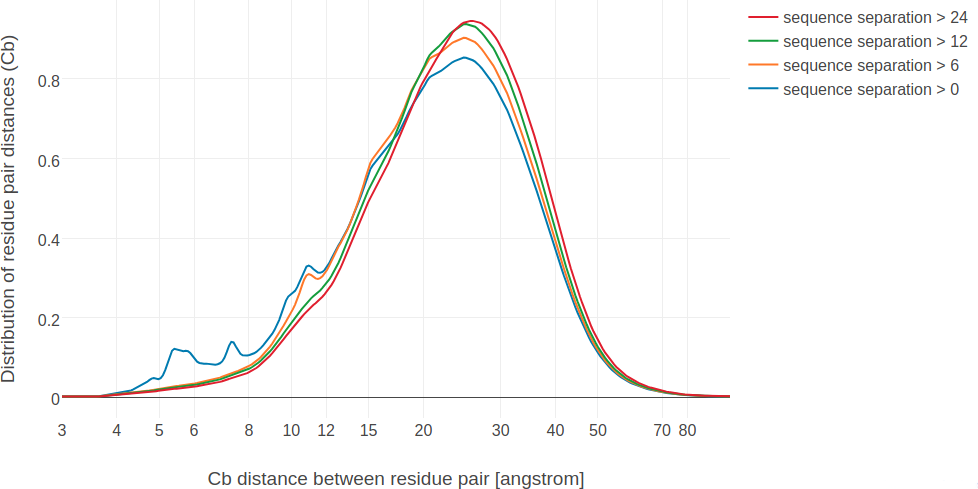
\includegraphics[width=1\linewidth]{img/dataset_statistics/Cb_distribution_all_data43579541_log} 

}

\caption{Distribution of residue pair \(\Cb\)
distances over 6741 proteins in the dataset (see Methods \ref{dataset})
at different minimal sequence separation thresholds.}\label{fig:Cb-distribution}
\end{figure}









\begin{figure}

{\centering 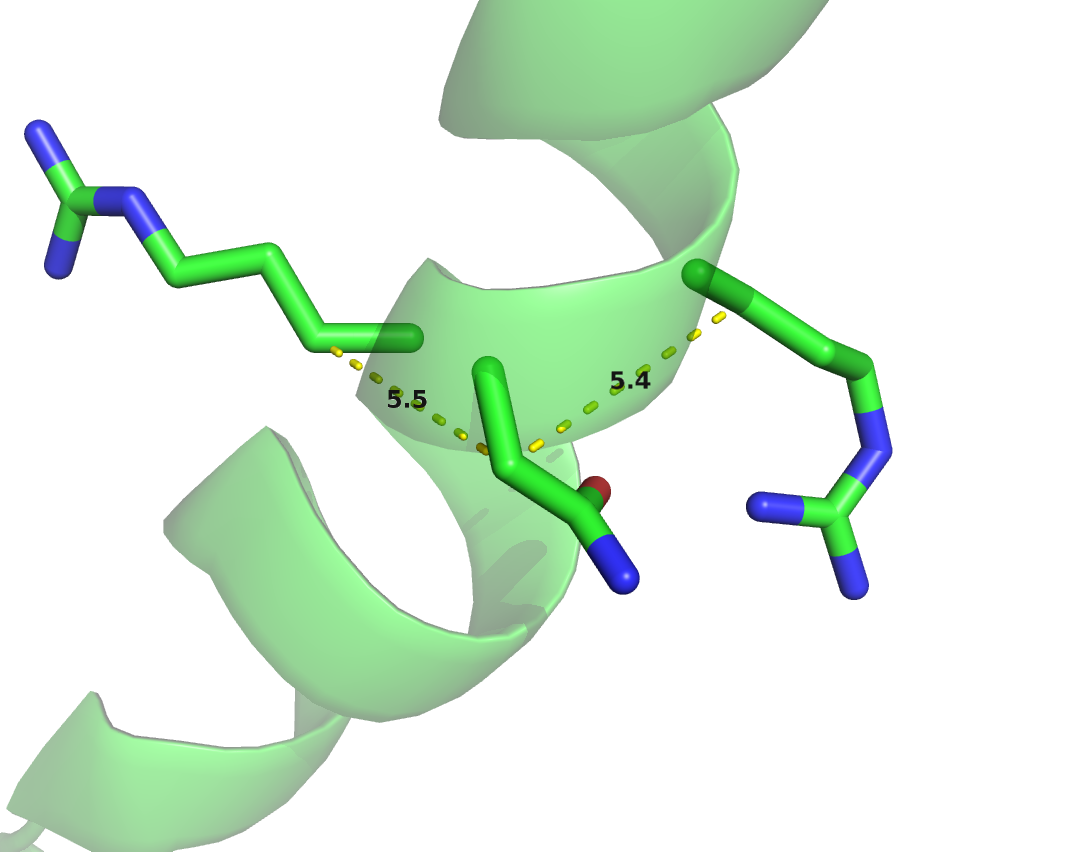
\includegraphics[width=0.4\linewidth]{img/dataset_statistics/cb_distribution_peak_5-6} 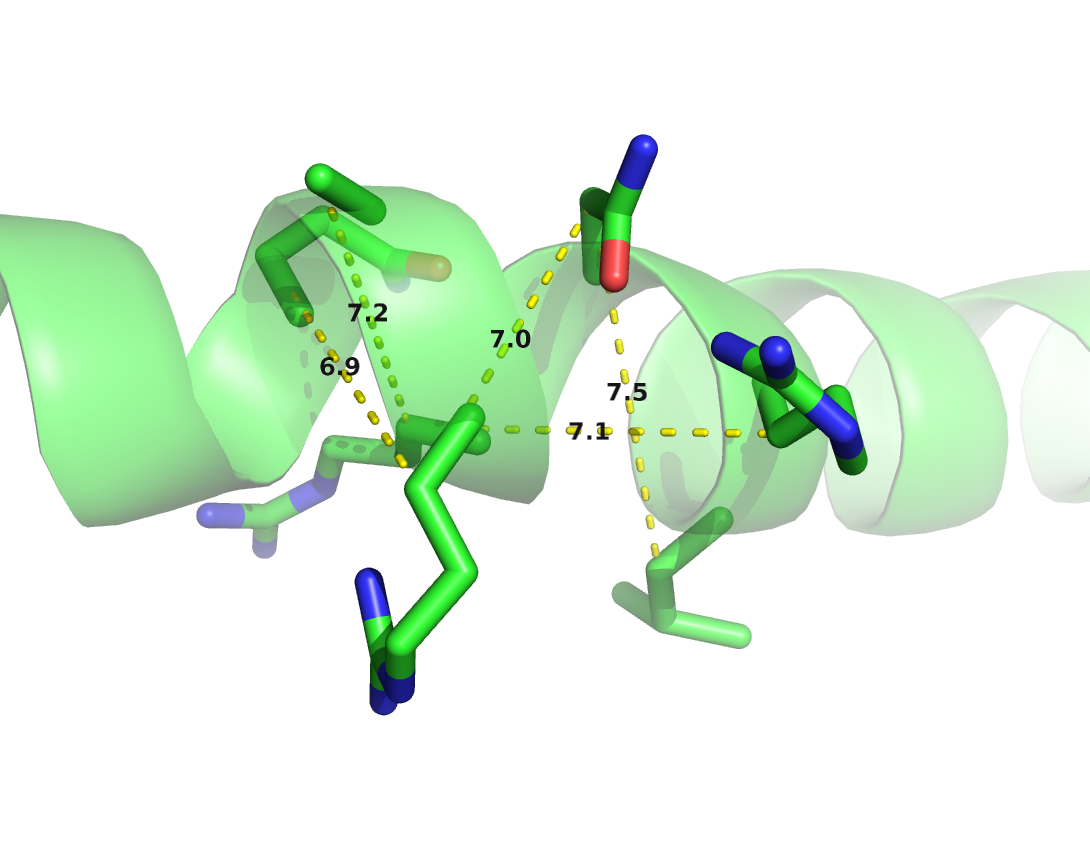
\includegraphics[width=0.4\linewidth]{img/dataset_statistics/cb_distribution_peak_7} 

}

\caption{\(\Cb\) distances between
neighboring residues in \(\alpha\)-helices. Left: Direct neighbors in
\(\alpha\)-helices have \(\Cb\) distances around \(5.4\angstrom\) due to
the geometrical constraints from \(\alpha\)-helical architecture. Right:
Residues separated by two positions (\(|i-j| = 2\)) are less
geometrically restricted to \(\Cb\) distances between \(7\angstrom\) and
\(7.5\angstrom\).}\label{fig:peaks-Cb-distribution}
\end{figure}

Commonly, sequence separation bins are applied to distuinguish short
(\(6 < |i-j| \le 12\)), medium (\(12 < |i-j| \le 24\)) and long range
(\(|i-j| > 24\)) contacts
{[}\protect\hyperlink{ref-Monastyrskyy2015}{90},\protect\hyperlink{ref-Monastyrskyy2014a}{170}{]}.
Especially long range contacts are of importance for structure
prediction as they are the most informative and able to constrain the
overal fold of a protein
{[}\protect\hyperlink{ref-Monastyrskyy2011}{169}{]}.

\subsection{Interpretation of Evaluation
Results}\label{interpretation-of-evaluation-results}

There are certain subtleties to be considered when interpreting contact
prediction evaluation results.

The rigid \(\Cb\) distance definition of a contact is a very rough
measure of true physical interactions between amino acid sidechains.
More importantly, interactions between sidechains depend on their
physico-chemical properties, on their orientation and different
environments within proteins (see section \ref{amino-acid-interactions})
{[}\protect\hyperlink{ref-Bettsa}{173}{]}. A simple \(\Cb\) distance
threshold not only misses to reflect biological interaction preferences
of amino acids but also provides a questionable gold-standard for
benchmarking. Other distance thresholds and definitions for physical
contacts (e.g minimal atomic distances or distance between functional
groups) have been studied as well. In fact, Duarte and colleagues found
that using a \(\Cb\) distance threshold between 9\(\angstrom\) and
11\(\angstrom\) yields optimal results when predicting the 3D structure
from the respective contacts
{[}\protect\hyperlink{ref-Duarte2010}{41}{]}. Anishchenko and colleagues
analysed false positive predictions with respect to a minimal atom
distance threshold \(< 5 \angstrom\), as they found that this cutoff
optimally defines direct physical interactions of residue pairs
{[}\protect\hyperlink{ref-Anishchenko2017}{174}{]}.

Another issue concerns structural variation within a protein family.
Evolutionary couplings are inferred from all family members in the
\protect\hyperlink{abbrev}{MSA} and therefore predicted contacts might
be physical contacts in one family member but not in another.
Anishchenko et al. could show that more than \(80\%\) of false positives
at intermediate distances (minimal heavy atom distance
5-15\(\angstrom\)) are true contacts in at least one homolog structure
{[}\protect\hyperlink{ref-Anishchenko2017}{174}{]}. Therefore, choosing
the right trade-off between sensitivity and specificity when generating
alignments is a crucial step as well as choosing the target protein
structure for evaluation.

Finally, an important aspect not considered in the standard benchmarks
is the spread of predicted contacts. It is perfectly possible to improve
precison of predicted contacts without translating this improvement to
better structural models. The reason being that structurally redundant
contacts, that is contacts in the immediate sequence neighborhood of
other contacts, do not give additional information to constrain the fold
{[}\protect\hyperlink{ref-Marks2011}{38},\protect\hyperlink{ref-Kim2014}{40},\protect\hyperlink{ref-Jones2015}{80}{]}.
For example, given a contact between residues \(i\) and \(j\), there is
hardly an added value knowing that there is a contact between residues
\(i\!+\!1\) and \(j\!+\!1\) when it comes to predicting the overal
topology. This observation is highly relevant for deep learning methods
due to their unique ability to abstract higher order interactions and
recognize contact patterns. Several measures of the contact spread have
been developed, like the mean euclidian distance between true and
predicted contacts, but are not commonly evaluated yet
{[}\protect\hyperlink{ref-Marks2011}{38},\protect\hyperlink{ref-DeOliveira2016}{144}{]}.

\section{Challenges for Coevolutionary Inference}\label{challenges}

Coevolution methods face several challenges when interpreting the
covariation signals obtained from a \protect\hyperlink{abbrev}{MSA}.
Some of these challenges have been successfully met (e.g.~disentangling
transitive effects with global statistical models), others are still
open or open up new perspectives, such as dissecting different sources
of coevolution signals.

\subsection{Phylogenetic Effects as a Source of
Noise}\label{phylogenetic-effects-as-a-source-of-noise}

Sequences in \protect\hyperlink{abbrev}{MSAs} do not represent
independent samples of a protein family. In fact, there is selection
bias from sequencing species of special interest (e.g human pathogens)
or sequencing closely related species, e.g multiple strains. This uneven
sampling of a protein family's sequence space leaves certain regions
unexplored whereas others are statistically overrepresented
{[}\protect\hyperlink{ref-Morcos2011}{95},\protect\hyperlink{ref-Cocco2017}{96},\protect\hyperlink{ref-Marks2012}{175}{]}.
Furthermore, due to their evolutionary relationship, sequences of a
protein family have a complicated dependence structure. Closely related
sequences can cause spurious correlations between positions, as there
was not sufficient time for the sequences to diverge from their common
ancestor
{[}\protect\hyperlink{ref-Gouveia_Oliveira2007}{57},\protect\hyperlink{ref-Lapedes1999}{61},\protect\hyperlink{ref-Burger2010}{62}{]}.
Figure \ref{fig:phylogenetic-effect} illustrates a simplified example,
where dependence of sequences due to phylogeny leads to a covariation
signal. To reduce the effects of redundant sequences, a popular sequence
reweighting strategy has been found to improve contact prediction
performance, where every sequence receives a weight that is the inverse
of the number of similar sequences according to an identity threshold
(see section \ref{seq-reweighting})
{[}\protect\hyperlink{ref-Jones2012}{65},\protect\hyperlink{ref-Morcos2011}{95},\protect\hyperlink{ref-Cocco2017}{96},\protect\hyperlink{ref-Buslje2009}{176}{]}.






\begin{figure}

{\centering 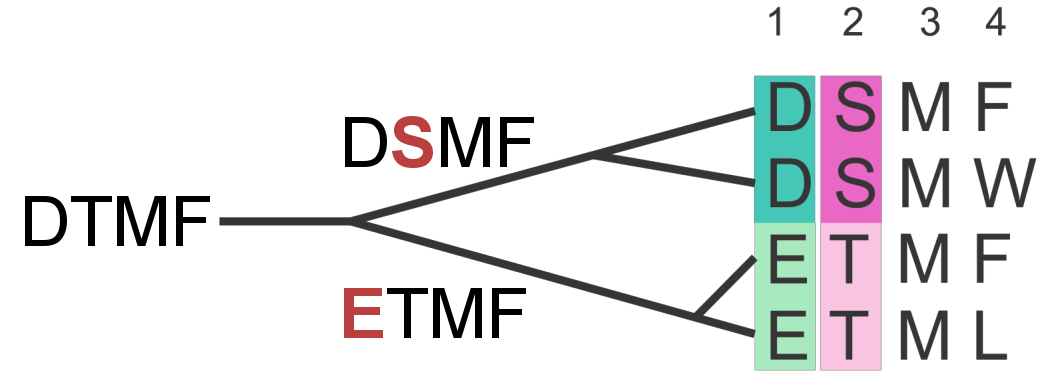
\includegraphics[width=0.6\linewidth]{img/intro/phylogenetic_effect} 

}

\caption{The phylogenetic dependence of closely
related sequences can produce covariation signals. Here, two independent
mutation events (highlighted in red) in two branches of the tree result
in a perfect covariation signal for two positions.}\label{fig:phylogenetic-effect}
\end{figure}

\subsection{Entropic Effects as a Source of
Noise}\label{entropic-effects-as-a-source-of-noise}

Another source for noise is entropy bias that is closely linked to
phylogenetic effects. By nature, methods detecting signals from
correlated mutations rely on a certain degree of covariation between
sequence positions {[}\protect\hyperlink{ref-Burger2010}{62}{]}. Highly
conserved interactions pose a conceptual challenge, as changes from one
amino acid to another cannot be detected if sequences do not vary. This
results in generally higher co-evolution signals from positions with
high entropy and underestimated signals for highly conserved
interactions {[}\protect\hyperlink{ref-Fodor2004}{55}{]}. Several
heuristics have been proposed to reduce entropy effects, such as
Row-Column-Weighting (RCW)
{[}\protect\hyperlink{ref-Gouveia_Oliveira2007}{57}{]} or Average
Product Correction (APC) {[}\protect\hyperlink{ref-Dunn2008}{58}{]} (see
section \ref{post-processing-heuristics}).

\subsection{Finite Sampling Effects}\label{finite-sampling-effects}

Spurious correlations can arise from random statistical noise and blur
true co-evolution signals especially in low data scenarios.
Consequently, false positive predictions attributable to random noise
accumulate for protein families comprising low numbers of homologous
sequences. This relationship was confirmed in many studies and as a rule
of thumb it has been argued that proteins with \(L\) residues need at
least \emph{5L} sequences in order to obtain confident predictions that
can bet used for protein structure prediction
{[}\protect\hyperlink{ref-Kamisetty2013}{102},\protect\hyperlink{ref-Marks2012}{175}{]}.
Recently it was shown that precision of predicted contacts saturates for
protein families with more than \(10^3\) diverse sequences and that
precision is only dependent on protein length for families with small
number of sequences {[}\protect\hyperlink{ref-Anishchenko2017}{174}{]}.

Interesting targets for contact prediction are protein families without
any associated structural information. As can be seen in Figure
\ref{fig:pfam}, those protein families generally comprise low numbers of
homologous sequences with a median of 185 sequences per family and are
thus susceptible to finite sampling effects.

With the rapidly increasing size of protein sequence databases (see
section \ref{general-intro}) the number of protein families with enough
sequences for accuarate contact predictions will increase steadily
{[}\protect\hyperlink{ref-Kamisetty2013}{102},\protect\hyperlink{ref-TheUniProtConsortium2013}{177}{]}.
Nevertheless, because of the already mentioned sequencing biases, better
and more sensitive statistical models are indespensible to extend the
applicability domain of coevolutionary methods.








\begin{figure}

{\centering 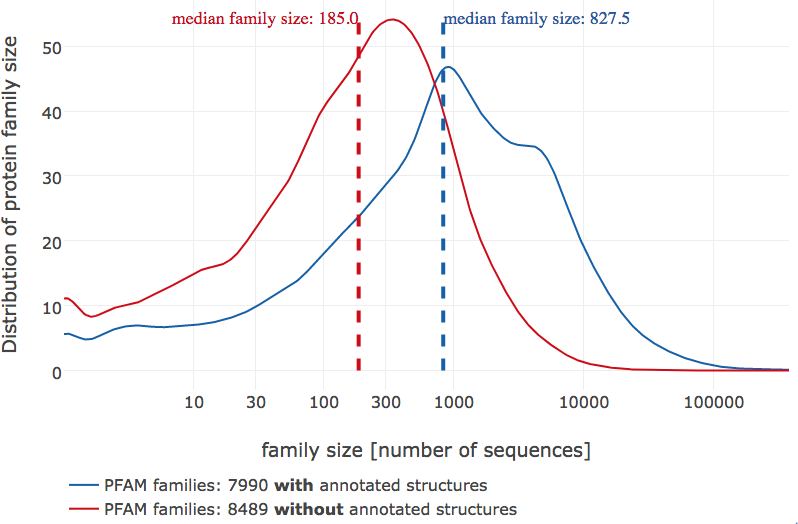
\includegraphics[width=0.9\linewidth]{img/pfam_pdb_notitle} 

}

\caption{Distribution of PFAM family sizes. Less than half of
the families in PFAM (7990 compared to 8489 families) do not have an
annotated structure. The median family size in number of sequences for
families with and without annotated structures is 185 and 827
respectively. Data taken from PFAM 31.0 (March 2017, 16712 entries)
{[}\protect\hyperlink{ref-Finn2016}{178}{]}.}\label{fig:pfam}
\end{figure}

\subsection{Multiple Sequence
Alignments}\label{multiple-sequence-alignments}

A correct \protect\hyperlink{abbrev}{MSA} is the essential starting
point for coevolution analysis as incorrectly aligned residues will
confound the true signal. Highly sensitive and accurate alignment tools
such as HHblits generate high quality alignments suitable for contact
prediction {[}\protect\hyperlink{ref-Remmert2012}{179}{]}. However,
there are certain subtleties to be kept in mind when generating
alignments.

For example, proteins with repeated stretches of amino acids or with
regions of low complexity are notoriously hard to align. Especially,
repeat proteins have been found to produce many false positive contact
predictions {[}\protect\hyperlink{ref-Anishchenko2017}{174}{]}.
Therefore, \protect\hyperlink{abbrev}{MSAs} need to be generated with
great care and covariation methods need to be tailored to these specific
types of proteins
{[}\protect\hyperlink{ref-Espada2014}{180},\protect\hyperlink{ref-Toth-Petroczy2016}{181}{]}.

Furthermore, sensitivity of sequence search is critically dependent on
the research question at hand and on the protein family under study.
Many diverse sequences in general increase precision of predictions
{[}\protect\hyperlink{ref-Ashkenazy2009}{171},\protect\hyperlink{ref-Avila-Herrera2015a}{182}{]}.
However, deep alignments can capture coevolutionary signals from
different subfamilies {[}\protect\hyperlink{ref-Uguzzoni2017}{149}{]}.
If only a specific subfamily is of interest, many false predictions
might arise from strong coevolutionary signals specific to another
subfamily that constitutes a prominent subset in the alignment
{[}\protect\hyperlink{ref-Franceus2016}{166}{]}. Therefore, a trade-off
between specificity and diversity of the alignment is required to reach
optimal results {[}\protect\hyperlink{ref-Hopf2012}{119}{]}.

Another intrinsic characteristic of \protect\hyperlink{abbrev}{MSAs} are
repeated stretches of gaps that result from commonly utilized
gap-penalty schemes assigning large penalties to insert a gap and lower
penalties to gap extensions. Most statistical coevolution models for
contact prediction treat gaps as the 21st amino acid. This introduces an
imbalance as gaps and amino acids express different behaviours which can
result in gap-induced artefacts
{[}\protect\hyperlink{ref-Feinauer2014}{110}{]}.

\subsection{Alternative Sources of
Coevolution}\label{alternative-sources-of-coevolution}

Coevolutionary signals can not only arise from intra-domain contacts,
but also from other sources, like homo-oligomeric contacts, alternative
conformations, ligand-mediated interactions or even contacts over
hetero-oligomeric interfaces (see Figure \ref{fig:sources-coevolution})
{[}\protect\hyperlink{ref-Marks2012}{175}{]}. With the objective to
predict physical contacts it is therefore necessary to identify and
filter these alternative sources of coevolutionary couplings.








\begin{figure}

{\centering 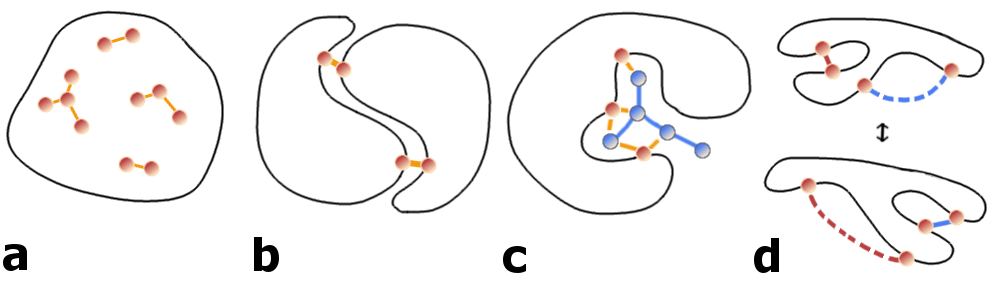
\includegraphics[width=0.9\linewidth]{img/intro/sources_of_coevolution} 

}

\caption{Possible sources of coevolutionary
signals. \textbf{a)} Physical interactions between intra-domain
residues. \textbf{b)} Interactions across the interface of predominantly
homo-oligomeric complexes. \textbf{c)} Interactions mediated by ligands
or metal atoms. \textbf{d)} Transient interactions due to conformational
flexibility.}\label{fig:sources-coevolution}
\end{figure}

Many proteins form homo-oligomers with evolutionary conserved
interaction surfaces (Figure \ref{fig:sources-coevolution} b). Currently
it is hard to reliably distinguish intra- and inter-molecular contacts
{[}\protect\hyperlink{ref-Uguzzoni2017}{149}{]}. Anishchenko et al.
found that approximately one third of strong co-evolutionary signals
between residue pairs at long distances (minimal heavy atom distance
\textgreater{}15\(\angstrom\)) can be attributed to interactions across
homo-oligomeric interfaces
{[}\protect\hyperlink{ref-Anishchenko2017}{174}{]}. Several studies
specifically analysed co-evolution across homo-oligomeric interfaces for
proteins of known structure by filtering for residue pairs with strong
couplings at long distances
{[}\protect\hyperlink{ref-Hopf2012}{119},\protect\hyperlink{ref-Wang2015}{125},\protect\hyperlink{ref-Uguzzoni2017}{149},\protect\hyperlink{ref-Sutto2015}{152},\protect\hyperlink{ref-Jana2014}{153},\protect\hyperlink{ref-Lee2009}{183}{]}
or used co-evolutionary signals to predict homo-dimeric complexes
{[}\protect\hyperlink{ref-DosSantos2015a}{150}{]}.

It has been proposed that co-evolutionary signals can also arise from
ligand or atom mediated interactions between residues or from critical
interactions in intermediate folding states (Figure
\ref{fig:sources-coevolution} c)
{[}\protect\hyperlink{ref-Buslje2009}{176},\protect\hyperlink{ref-Ovchinnikov2015b}{184}{]}.
Confirming this hypothesis, a study showed that the cumulative strength
of couplings for a particular residue can be used to predict functional
sites
{[}\protect\hyperlink{ref-Hopf2012}{119},\protect\hyperlink{ref-Marks2012}{175}{]}.

Another important aspect is conformational flexibility (Figure
\ref{fig:sources-coevolution} c). PDB structures used to evaluate
coevolution methods represent only rigid snapshots taken in an unnatural
crystalline environment. Yet proteins possess huge conformational
plasticity and can adopt distinct alternative conformations or adapt
shape when interacting with other proteins in an induced fit manner
{[}\protect\hyperlink{ref-Noel2016}{185}{]}. Several studies
demonstrated successfully that coevolutionary signals can capture
interactions specific to different distinct conformations
{[}\protect\hyperlink{ref-Morcos2011}{95},\protect\hyperlink{ref-Hopf2012}{119},\protect\hyperlink{ref-Sfriso2016}{151},\protect\hyperlink{ref-Jana2014}{153}{]}.

\chapter{Interpretation of Coupling
Matrices}\label{interpreting-coupling-matrices}

Contact prediction methods learning a \emph{Potts model} for the
\protect\hyperlink{abbrev}{MSA} of a protein familiy, map the inferred
20 x 20 dimensional coupling matrices \(w_{ij}\) onto scalar values to
obtain contact scores for each residue pair as outlined in section
\ref{post-processing-heuristics}. As a result, the full information
contained in coupling matrices is lost, such as the contribution of
individual couplings \(\wijab\), whether a coupling is positive or
negative, higher order dependencies between couplings or possibly
biological meaningful signals. The following sections give some
intuition for the information contained in coupling matrices.

\section{Single Coupling Values Carry Evidence of
Contacts}\label{correlation-between-couplings-and-class}

Given the success of \protect\hyperlink{abbrev}{DCA} methods, it is
clear that the inferred couplings \(\wij\) are good indicators of
spatial proximity for residue pairs. As described in section
\ref{post-processing-heuristics}, a contact score \(C_{i,j}\) for a
residue pair \((i,j)\) is commonly computed as the Frobenius norm over
the coupling matrix,
\(C_{i,j}=||\wij||_2 = \sqrt{\sum_{a,b=1}^{20} {\wijab}^2}\).

The plots in Figure \ref{fig:sq-coupling-correlation} show the
correlation of squared coupling values \({\wijab}^2\) with binary
contact class (contact=1, non-contact=0) and the standard deviation of
squared coupling values \({\wijab}^2\) for contacts computed on a
dataset of 100.000 residue pairs per class (for details see methods
section \ref{method-coupling-correlation}). All couplings have a weak
positive class correlation, meaning the stronger the squared coupling
value, the more likely a contact can be inferred. Correlation is weak
because most couplings \(\wijab\) are close to zero since typically only
few amino acid pairings per residue pair carry evidence and produce a
signal. Generally, couplings that involve an aliphatic amino acid such
as isoleucine (I), leucine (L), valine (V) or an alanine (A) express the
strongest class correlation. In contrast, cysteine pairs (C-C) or pairs
involving only the charged residus arginine (R), glutamic acid (E),
lysine (K) or aspartic acid (D) correlate only weakly with contact
class. Interestingly, for residue pairs being in physical contact, C-C
and couplings involving charged residues have the highest
standard-deviation among all couplings as can be seen in the right plot
in Figure \ref{fig:sq-coupling-correlation}. Standard deviation of
squared coupling values from non-contacts shows no relevant patterns and
is on average one magnitude smaller than for the contact class (see
Appendix Figure \ref{fig:stdev-squared-couplings-noncontacts}).










\begin{figure}

{\centering 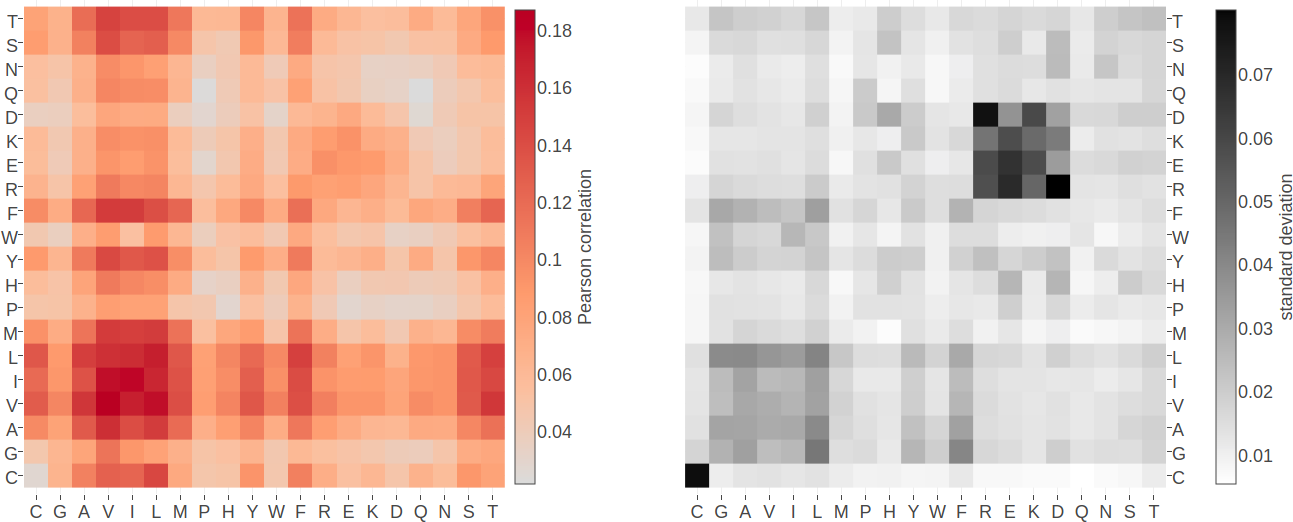
\includegraphics[width=1\linewidth]{img/coupling_matrix_analysis/combi_squared_couplings_correlation_and_stddev_heatmap_notitle} 

}

\caption{\textbf{Left} Pearson correlation of squared
coupling values \((\wijab)^2\) with contact class (contact=1,
non-contact=0). \textbf{Right} Standard deviation of squared coupling
values for residue pairs in contact. Dataset contains 100.000 residue
pairs per class (for details see methods section
\ref{method-coupling-correlation}). Amino acids are abbreviated with
one-letter code and they are broadly grouped with respect to
physico-chemical properties listed in Appendix \ref{amino-acids}.}\label{fig:sq-coupling-correlation}
\end{figure}

Different couplings are of varying importance for contact inference and
have distinct characteristics. When looking at the raw coupling values
(without squaring), these charateristics become even more pronounced.
The plots in Figure \ref{fig:coupling-correlation} show the correlation
of raw coupling values \(\wijab\) with contact class and the standard
deviation of coupling values for contacts. Standard deviation of
coupling values for non-contacts shows no relevant patterns and is on
average half as big as for the contact class (see Appendix Figure
\ref{fig:stdev-raw-couplings-noncontacts}). Interestingly, in contrast
to the findings for squared coupling values, couplings for charged
residue pairs, involving arginine (R), glutamic acid (E), lysine (K) and
aspartic acid (D), have the strongest class correlation (positive and
negative), whereas aliphatic coupling pairs correlate to a much lesser
extent. This implies that squared coupling value is a better indicator
of a contact than the raw signed coupling value for aliphatic couplings.
On the contrary, the raw signed coupling values for charged residue
pairs are much more indicative of a contact than the magnitude of their
squared values. Raw couplings for cysteine (C-C) pairs, proline (P) and
tryptophane (W) correlate only weakly with contact class. For these
pairs neither a squared coupling value nor the raw coupling value seems
to be a good indicator for a contact.










\begin{figure}
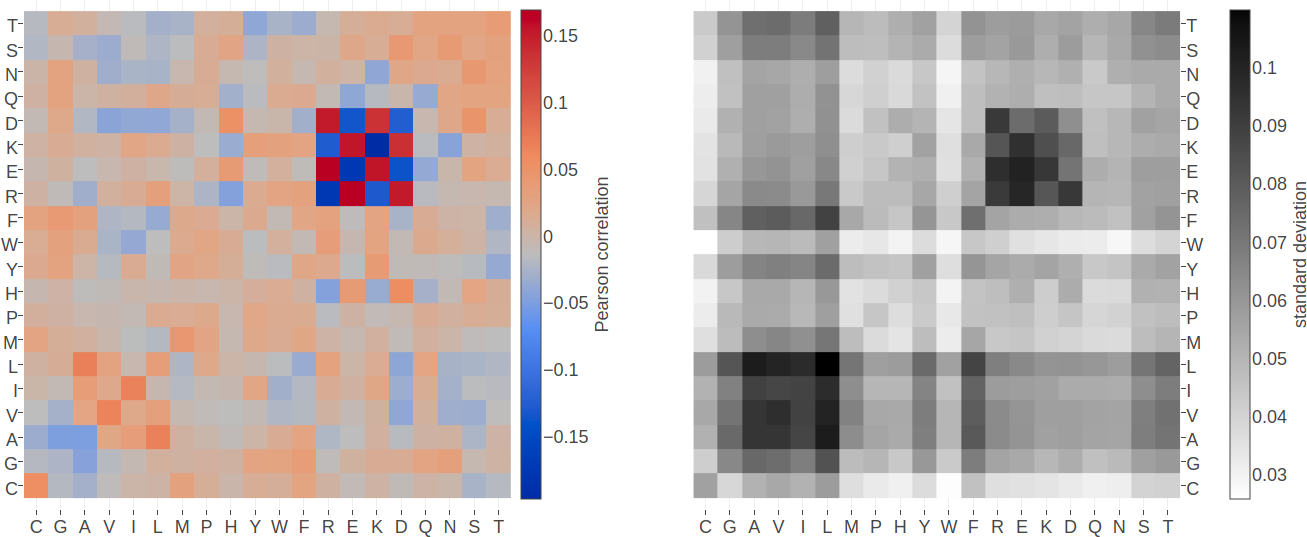
\includegraphics[width=1\linewidth]{img/coupling_matrix_analysis/combi_couplings_correlation_and_stddev_heatmap_notitle} \caption{\textbf{Left} Pearson correlation of
raw signed coupling values \(\wijab\) with contact class (contact=1,
non-contact=0). \textbf{Right} Standard deviation of coupling values for
residue pairs in physical contact. Dataset contains 100.000 residue
pairs per class (for details see section
\ref{method-coupling-correlation}). Amino acids are abbreviated with
one-letter code and they are broadly grouped with respect to
physico-chemical properties listed in Appendix \ref{amino-acids}.}\label{fig:coupling-correlation}
\end{figure}

Looking only at correlations can be misleading if there are non-linear
patterns in the data, for example higher order dependencies between
couplings. For this reason it is advisable to take a more detailed view
at coupling matrices and the distributions of their values.

\section{Physico-Chemical Fingerprints in Coupling
Matrices}\label{physico-chemical-fingerprints-in-coupling-matrices}

The correlation analysis of coupling matrices in the last section
revealed that certain couplings are more indicative of a contact than
others. Individual coupling matrices for a residue pair that is in
physcial contact often display striking patterns that agree with the
previous findings. These patterns allow a biological interpretation of
the coupling values that reveal details of the physico-chemical
interdependency between both residues.

Figure \ref{fig:coupling-matrix-ionic-interaction} visualizes the
inferred coupling matrix and single potentials \(\vi\) and \(\vj\) for a
residue pair \((i,j)\) computed with the pseudo-likelihood method. The
single potentials \(\via\) and \(\vja\) describe the tendency for each
amino acid \(a\) to appear at positions \(i\) and \(j\), and the
couplings \(\wijab\) describe the tendency of amino acid \(a\) at
position \(i\) to co-occur with amino acid \(b\) at position \(j\). A
cluster of strong coupling values can be observed for the couplings
between the charged residues glutamic acid (E), aspartic acid (D),
lysine (K) and arginine (R) and the polar residue glutamine (Q).
Positive coupling values arise between positively charged residues (K,
R) and negatively charged residues (E, D), whereas couplings between
equally charged residues have negative values. These exemplary couplings
(E-R, E-K, K-D) perfectly reflect the interaction preference for
residues forming salt bridges. Indeed, in the protein structure the
first residue (E) forms a salt bridge with the second residue (R) as can
be seen in the left plot in Figure \ref{fig:coupling-matrix-pymol}.














\begin{figure}
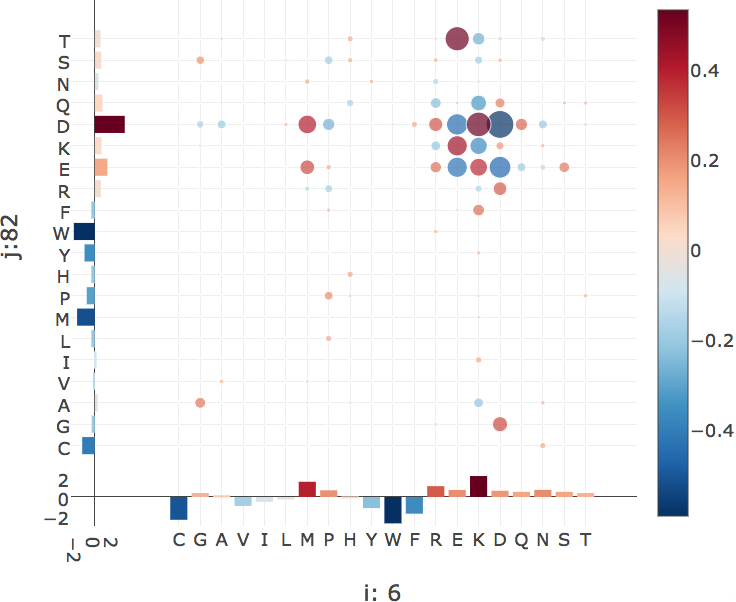
\includegraphics[width=1\linewidth]{img/coupling_matrix_analysis/coupling_matrix_1a9xA05_6_82_notitle} \caption{Couplings \(\wijab\) and
single potentials \(\via\) and \(\vja\) computed with pseudo-likelihood
for residues 6 and 82 in protein chain 1a9x\_A\_05. The matrix shows the
20x20 couplings \(\wijab\) with color representing coupling strength and
direction (red = positive coupling value, blue = negative coupling
value) and diameter of bubbles representing absolute coupling value
\(|\wijab|\). Bars at the x-axis and y-axis correspond to the
\emph{Potts} model single potentials \(\vi\) and \(\vj\) respectively.
Color reflects the value of single potentials. Amino acids are
abbreviated with one-letter code and they are broadly grouped with
respect to physico-chemical properties listed in Appendix
\ref{amino-acids}.}\label{fig:coupling-matrix-ionic-interaction}
\end{figure}

Figure \ref{fig:coupling-matrix-hydrophobic-interaction} visualizes the
coupling matrix for a pair of hydrophobic residues. Hydrophobic
pairings, such as alanine (A) - isoleucine (I), or glycine (G) -
isoleucine (I) have strong coupling values but the couplings also
reflect a sterical constraint. Alanine is a small hydrophobic residue
and it is favoured at both residue positions: it has strong positive
single potentials \(\vi(A)\) and \(\vj(A)\) and strong positive
couplings with isoleucine (I), leucine (L) and methionine (M). But
alanine is disfavoured to appear at both positions at the same time
since the A-A coupling is negative. Figure
\ref{fig:coupling-matrix-pymol} illustrates the location of the two
residues in the protein core. Here, hydrophobic residues are densely
packed and the limited space allows for only small hydrophobic residues.














\begin{figure}
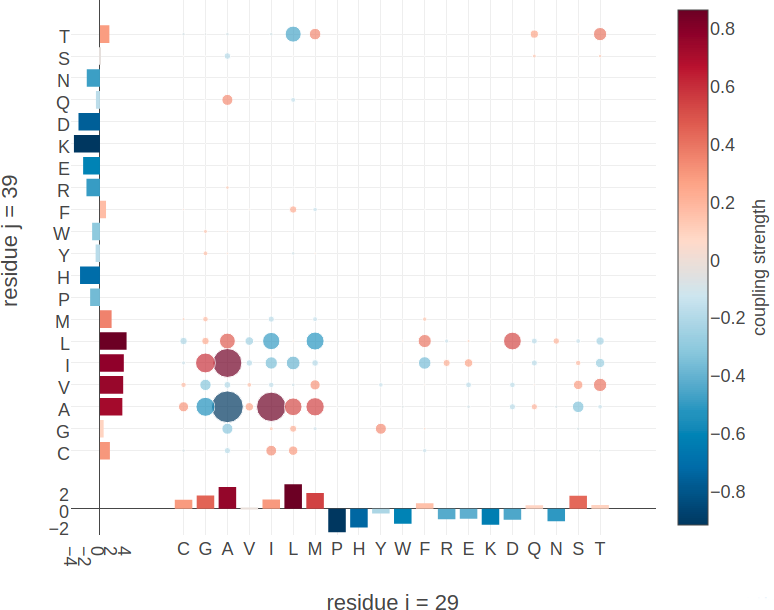
\includegraphics[width=1\linewidth]{img/coupling_matrix_analysis/coupling_matrix_1ae9A00_29_39_notitle} \caption{Couplings
\(\wijab\) and single potentials \(\via\) and \(\vja\) computed with
pseudo-likelihood for residues 29 and 39 in protein chain 1ae9\_A\_00.
The matrix shows the 20x20 couplings \(\wijab\) with color representing
coupling strength and direction (red = positive coupling value, blue =
negative coupling value) and diameter of bubbles representing absolute
coupling value \(|\wijab|\). Bars at the x-axis and y-axis correspond to
the \emph{Potts} model single potentials \(\vi\) and \(\vj\)
respectively. Color reflects the value of single potentials. Amino acids
are abbreviated with one-letter code and they are broadly grouped with
respect to physico-chemical properties listed in Appendix
\ref{amino-acids}.}\label{fig:coupling-matrix-hydrophobic-interaction}
\end{figure}






\begin{figure}
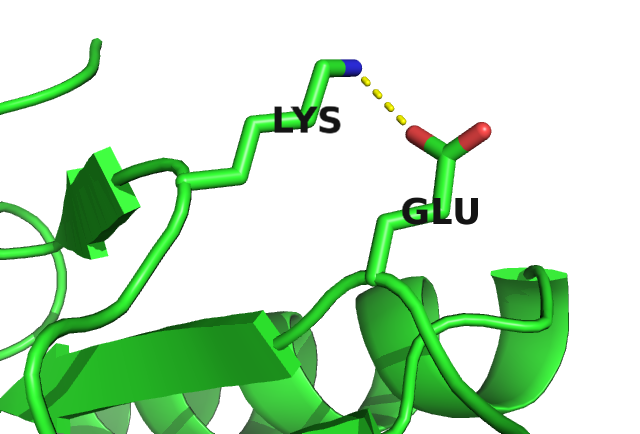
\includegraphics[width=0.5\linewidth]{img/coupling_matrix_analysis/1a9xA05_6_82} 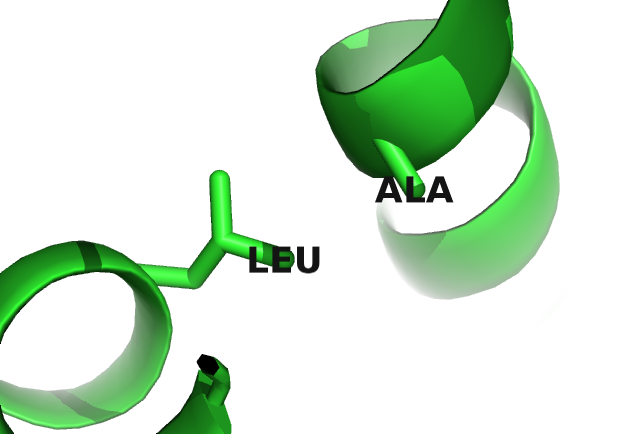
\includegraphics[width=0.5\linewidth]{img/coupling_matrix_analysis/1ae9A00_29_39} \caption{Interactions between protein side
chains. \textbf{Left}: residue 6 (E) forms a salt bridge with residue 82
(R) in protein chain 1a9x\_A\_05. \textbf{Right}: residue 29 (A) and
residue 39 (L) within the hydrophobic core of protein chain 1ae9\_A\_00.}\label{fig:coupling-matrix-pymol}
\end{figure}

Many more biological interpretable signals can be identified from
coupling matrices, including pi-cation interactions (see Appendix
\ref{pi-cation}), aromatic-proline interactions (see Appendix
\ref{aromatic-proline}), sulfur-aromatic interactions or disulphide
bonds (see Appendix \ref{disulfide}).

Coucke and collegues performed a thorough quantitative analysis of
coupling matrices selected from confidently predicted residue pairs
{[}\protect\hyperlink{ref-Coucke2016}{186}{]}. They showed that
eigenmodes obtained from a spectral analysis of averaged coupling
matrices are closely related to physico-chemical properties of amino
acid interactions, like electrostaticity, hydrophobicity, steric
interactions or disulphide bonds. By looking at specific populations of
residues, like buried and exposed residues or residues from specific
protein classes (small, mainly \(\alpha\), etc), the eigenmodes of
corresponding coupling matrices are found to capture very characteristic
interactions for each class, e.g.~rare disulfide contacts within small
proteins and hydrophilic contacts between exposed residues. Their study
confirms the qualitative observations presented above that amino acid
interactions can leave characteristic physico-chemical fingerprints in
coupling matrices.

\section{Coupling Profiles Vary with Distance}\label{coupling-profiles}

Analyses in the previous sections showed that certain coupling values
correlate more or less strong with contact class and that coupling
matrices for contacts express biological meaningfull patterns.

More insights can be obtained by looking at the distribution of distinct
coupling values for contacts, non-contacts and arbitrary populations of
residue pairs. Figure \ref{fig:1d-coupling-profile-0-5} shows the
distribution of selected couplings for filtered residue pairs with
\(\Cb-\Cb\) distances \(< 5\angstrom\) (see methods section
\ref{method-coupling-profile} for details). The distribution of R-E and
E-E coupling values is shifted and skewed towards positive and negative
values respectively. This is in accordance with attracting electrostatic
interactions between the positively charged side chain of arginine and
the negatively charged side chain of gluatamic acid and also with
repulsive interactions between the two negatively charged glutamic acid
side chains.

Coupling values for cysteine pairs (C-C) have a broad distribution that
is skewed towards positive values, reflecting the strong signals
obtained from covalent disulphide bonds. The broad distribution for C-C,
R-E and E-E agrees with the observation in section
\ref{correlation-between-couplings-and-class} that these specific
coupling values have large standard deviations and that for charged
residue pairings the signed coupling value is a strong indicator of a
contact.

Hydrophobic pairs like V-I have an almost symmetric coupling
distribution, confirming the finding that the direction of coupling is
not indicative of a true contact whereas the strength of the coupling
is. The hydrophobic effect that determines hydrophobic interactions is
not specific or directed. Therefore, hydrophobic interaction partners
can commonly be substituted by other hydrophobic residues, which
explains the not very pronounced positive coupling signal compared to
more specific interactions, e.g ionic interactions. It is not clear
though, why hydrophobic pairs have an equally strong negative coupling
signal at this distance range because this speaks against the hypothesis
that hydrophobic pairs are commonly interchangeable. A vague explanation
could be that a location in the tighly packed protein core calls for
other very specific constraints, e.g.~sterical fit or contact number,
besides hydrophobic properties that are prohibitive for a particular
hydrophobic residue at a certain position.

The distribution of aromatic coupling values like F-W is slightly skewed
towards negative values, accounting for steric hindrance of their large
sidechains at small distances. The yet very pronounced positive coupling
signal for the bulky aromatic residues at this short distance range is
not clear. The bulky planar aromatic rings of two aromatic residues
often point away from each other when their \(\Cb\)-\(\Cb\) distances
are small to avoid steric hindrance (see Apendix Figure
\ref{fig:aromatic-residues-at-short-distances}). A positive coupling
signal might originate from other structural constraints from the local
environment affecting both sidechains, similar to the scenario
hypothetically explaining the negative coupling signal for hydrophobic
residues.











\begin{figure}

{\centering 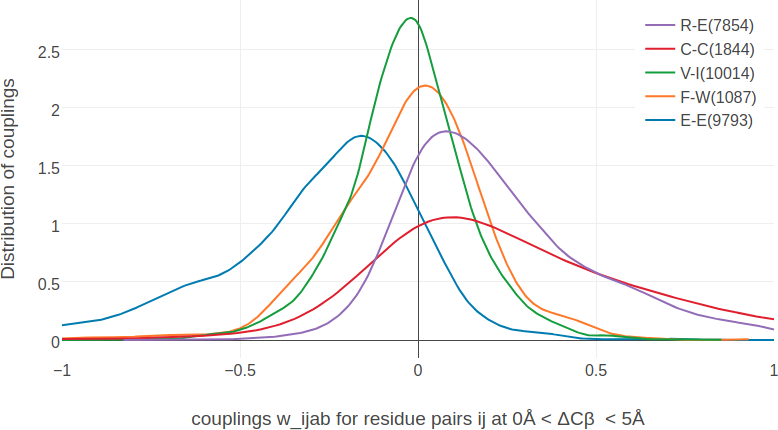
\includegraphics[width=1\linewidth]{img/coupling_matrix_analysis/1d_coupling_profile_0_5} 

}

\caption{Distribution of selected couplings
for filtered residue pairs with \(\Cb-\Cb\) distances \(< 5\angstrom\)
(see methods section \ref{method-coupling-profile} for details). Number
of coupling values used to determine the distribution is given in
brackets in the legend. \(\text{R-E}\) = couplings for arginine and
glutamic acid pairs, \(\text{C-C}\) = coupling for cystein residue
pairs, \(\text{V-I}\) = coupling for valine and isoleucine pairs,
\(\text{F-W}\) = coupling for phenylalanine and tryptophane pairs,
\(\text{E-E}\) = coupling for glutamic acid residue pairs.}\label{fig:1d-coupling-profile-0-5}
\end{figure}

In an intermediate \(\Cb\) distance range between \(8\angstrom\) and
\(12\angstrom\) the distributions for all coupling values are centered
close to zero and are less broad. The distributions are still shifted
and skewed, but less pronounced compared to the distributions at
\(\Cb-\Cb\) distances \(< 5\angstrom\). For aromatic pairs like F-W, the
distribution of coupling values has very long tails, suggesting rare but
strong couplings for aromatic side chains at this distance.








\begin{figure}
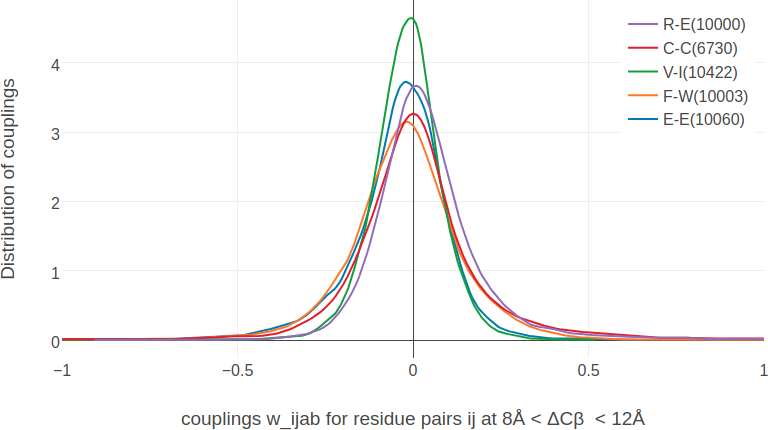
\includegraphics[width=1\linewidth]{img/coupling_matrix_analysis/1d_coupling_profile_8_12} \caption{Distribution of selected
couplings for filtered residue pairs with \(\Cb-\Cb\) distances between
\(8\angstrom\) and \(12 \angstrom\) (see methods section
\ref{method-coupling-profile} for details). Number of coupling values
used to determine the distribution is given in brackets in the legend.
Couplings are the same as in Figure \ref{fig:1d-coupling-profile-0-5}.}\label{fig:1d-coupling-profile-8-12}
\end{figure}

Figure \ref{fig:1d-coupling-profile-20-50} shows the distribution of
selected couplings for residue pairs far apart in the protein structure
(\(\Cb-\Cb\) distances \(> 20\angstrom\)).\\
The distribution for all couplings is centered at zero and has small
variance. Only for C-C coupling values, the distribution has a long tail
for positve values, presumably arising from the fact that the maximum
entropy model cannot distuinguish highly conserved signals of multiple
disulphide bonds within a protein. This observation also agrees with the
previous finding in section
\ref{correlation-between-couplings-and-class} that C-C coupling values,
albeit having large standard-deviations, correlate only weakly with
contact class. The same arguments apply to couplings of aromatic pairs
that have a comparably broad distribution and do not correlate strongly
with the contact class. The strong coevolution signals for aromatic
pairs even at high distance ranges might result from some kind of
cooperative effects. Aromatic residues are known to form network-like
structures in the protein core that stabilize protein structure
{[}\protect\hyperlink{ref-Burley1985}{187}{]}. An example is given in
Appendix Figure \ref{fig:aromatic-network}. A possible explanation might
be that the \emph{Potts model} is limited to learning single positions
and pairwise correlations. An extension to higher order couplings might
resolve these cooperative effects observed between residues in the
protein core.








\begin{figure}
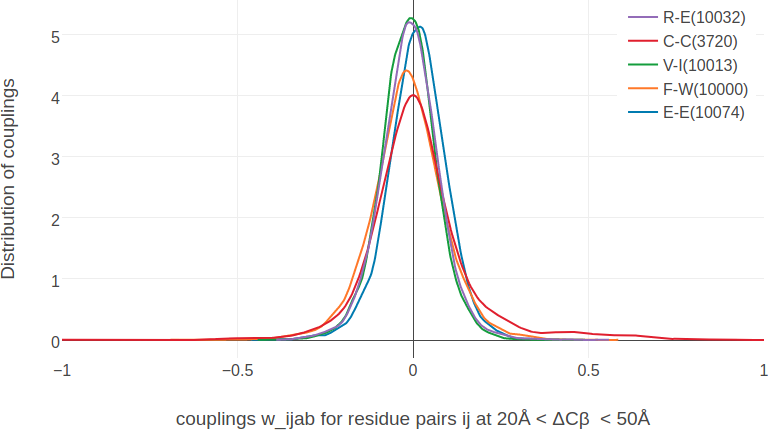
\includegraphics[width=1\linewidth]{img/coupling_matrix_analysis/1d_coupling_profile_20_50} \caption{Distribution of selected
couplings for filtered residue pairs with \(\Cb-\Cb\) distances between
\(20\angstrom\) and \(50\angstrom\) (see methods section
\ref{method-coupling-profile} for details). Number of coupling values
used to determine the distribution is given in brackets in the legend.
Couplings are the same as in Figure \ref{fig:1d-coupling-profile-0-5}.}\label{fig:1d-coupling-profile-20-50}
\end{figure}

\section{Higher Order Dependencies Between
Couplings}\label{higher-order-coupling-profiles}

The analyses in the previous sections focused on single coupling values
picked from the \(20 \times 20\)-dimensional coupling matrices \(\wij\).
As mentioned before, analysing only single dimensions might be
misleading when variables are dependent on each other and further
insights might be concealed in higher order relationships.
Unfortunately, it is not possible to reasonably visualize high
dimensional coupling matrices.

Exploring two dimensional coupling scatter plots strengthens the
observation that couplings matrices contain signals that reflect
biological relevant amino acid interactions. The plots in the top row in
Figure \ref{fig:2d-coupling-profiles-0-8} show the distribution of
couplings for filtered residue pairs with \(\Cb-\Cb\) distances
\(< 8\angstrom\) between the ionic pairings of E-R and R-E and between
the ionic pairing R-E and the equally charged residues E-E,
respectively. Coupling values for R-E and E-R are positively correlated
with predominantly positive values. This means when the amino acid pair
R-E is frequently observed at two positions \(i\) and \(j\), then it
also likely that the amino acid pair E-R can be frequently observed.
This situation indicates an important ionic interaction whereby the
location of the positively and negatively charged residue at position
\(i\) or \(j\) is irrelevant.

On the contrary, coupling values for R-E and E-E are negatively
correlated, with positive values for R-E and negative values for E-E.
This distribution can be interpreted with frequently occuring amino acid
pairs R-E at two positions \(i\) and \(j\) while at the same time the
amino acid pair E-E cannot be observed. Again, this situation coincides
with amino acid pairings that would be expected for an ionic
interaction.

The bottom left plot in Figure \ref{fig:2d-coupling-profiles-0-8} shows
the distribution between couplings for the hydrophobic pairings I-L and
V-I that is almost symmetric and broadly centered around zero. Coupling
distributions for residue pairs that are not physically interacting
(\(\Cb \gg 8 \angstrom\)) resemble the distribution for hydrophobic
pairings in that there is no correlation, but at high distance the
distributions are much tighter centered around zero (bottom right plot
in Figure \ref{fig:2d-coupling-profiles-0-8}).
















\begin{figure}
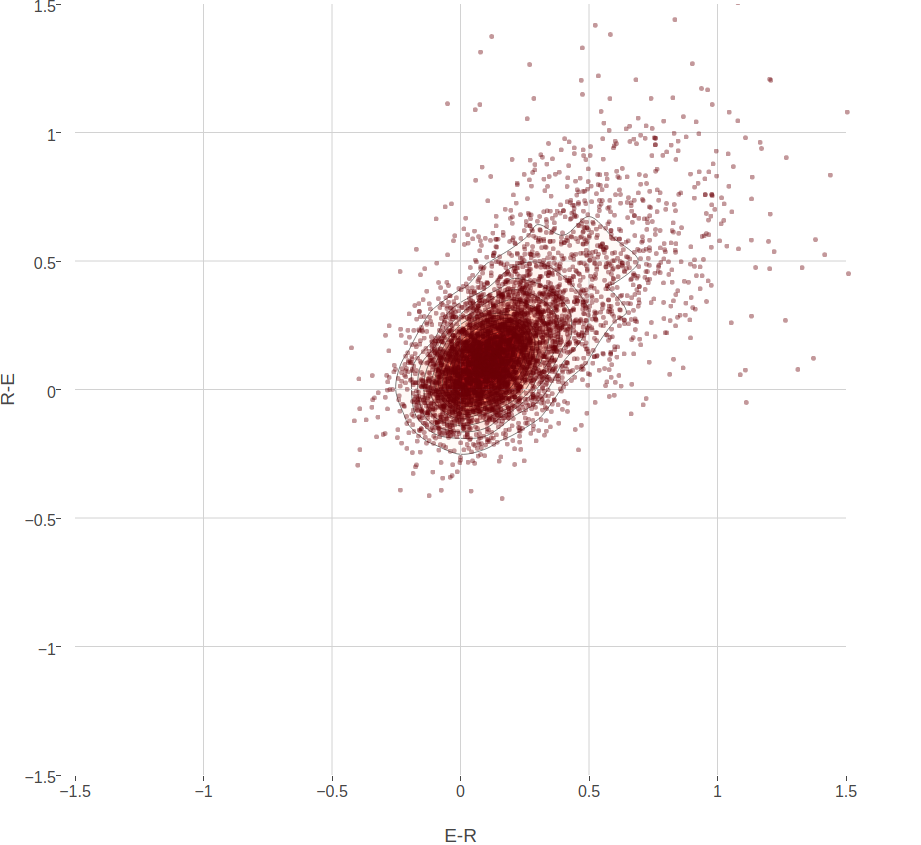
\includegraphics[width=0.5\linewidth]{img/coupling_matrix_analysis/pairwise_couplings_R-E_E-R_Cbdistance_0_8_notitle} 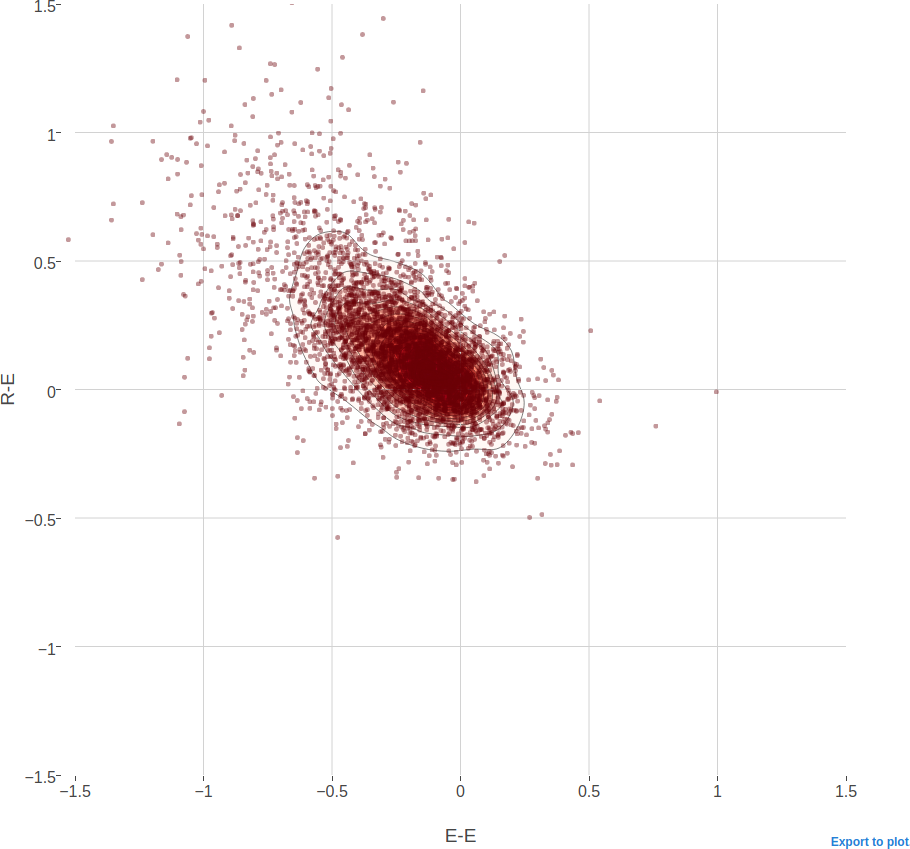
\includegraphics[width=0.5\linewidth]{img/coupling_matrix_analysis/pairwise_couplings_R-E_E-E_Cbdistance_0_8_notitle} 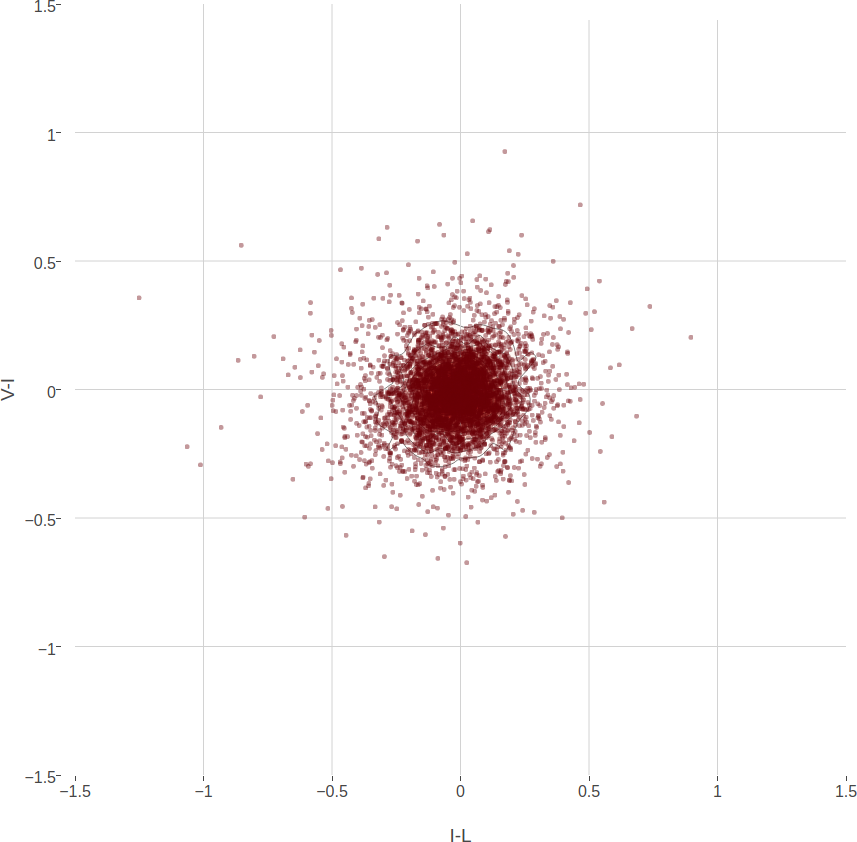
\includegraphics[width=0.5\linewidth]{img/coupling_matrix_analysis/pairwise_couplings_V-I_I-L_Cbdistance_0_8_notitle} 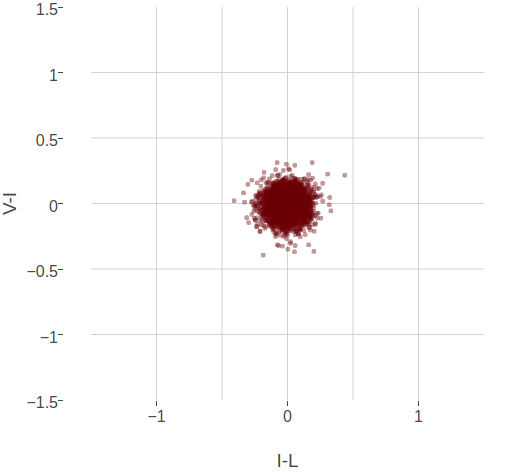
\includegraphics[width=0.5\linewidth]{img/coupling_matrix_analysis/pairwise_couplings_V-I_I-L_Cbdistance_20_50_notitle} \caption{Two-dimensional distribution of
approximately 10000 coupling values computed with pseudo-likelihood.
\textbf{Top Left} The 2-dimensional distribution of couplings E-R and
R-E for residue pairs with \(\Cb-\Cb\) distances \(< 8 \angstrom\) is
almost symmetric and the coupling values are positively correlated.
\textbf{Top Right} The 2-dimensional distribution of couplings E-R and
E-E for residue pairs with \(\Cb-\Cb\) distances \(< 8 \angstrom\) is
almost symmetric and the coupling values are negatively correlated.
\textbf{Bottom Left} The 2-dimensional distribution of couplings I-L and
V-I for residue pairs with \(\Cb-\Cb\) distances \(< 8 \angstrom\) is
symmetrically distributed around zero without visible correlation.
\textbf{Bottom Right} The 2-dimensional distribution of couplings I-L
and V-I for residue pairs with \(\Cb-\Cb\) distances \(> 20 \angstrom\)
is tighly distributed around zero.}\label{fig:2d-coupling-profiles-0-8}
\end{figure}

\chapter{Optimizing the Full
Likelihood}\label{optimizing-full-likelihood}

Section \ref{maxent} introduced the \emph{Potts model} for contact
prediction that is able to distinguish between directly and indirectly
coupled residue pairs by jointly modelling the probabilty of a protein
sequence over all residues. Maximum-likelihood inference of the model
parameters is numerically challenging due to the exponential complexity
of the partition function that normalizes the probability distribution.
Several approximate inference techniques for the full likelihood have
been developed trying to sidestep the exact computation of the partition
function. At this point in time, pseudo-likelihood is the most
successful approximate solution with regard to predicting
residue-residue contacts (see section \ref{pseudo-likelihood}). It has
been shown that the pseudo-likelihood is a consistent estimator to the
full likelihood in the limit of large amounts of data. However, it is
unclear whether it represents a good approximation when there is only
little data, in other words for small protein families that are the most
interesting targets for contact prediction (see Figure \ref{fig:pfam}).

While the partition function of the full likelihood cannot be
efficiently computed, it is possible to approximate the gradient of the
full likelihood with an approach called \emph{contrastive divergence}
that makes use of \protect\hyperlink{abbrev}{MCMC} sampling techniques
{[}\protect\hyperlink{ref-Hinton2002}{188}{]}. This section elaborates
on how \emph{contrastive divergence} can be used to optimize the full
likelihood with gradient descent techniques. Furthermore, two aspects of
the underlying \emph{Potts model}, namely gap treatment and the choice
of regularization, have been refined which is explained in detail in
methods section \ref{potts-full-likelihood}.

\section{Approximating the Gradient of the Full Likelihood with
Contrastive Divergence}\label{full-likelihood-gradient}

The gradient of the regularized full log likelihood with respect to the
couplings \(\wijab\) can be written as

\begin{equation}
    \frac{\partial \LLreg}{\partial \wijab} = \; N_{ij} q(x_i \eq a, x_j=b) - N_{ij} \; p(x_i \eq a, x_j \eq b | \v,\w) - \lambda_w \wijab  \; ,
\label{eq:gradient-wijab-full-likelihood-approx}
\end{equation}

where \(N_{ij} q(x_i \eq a, x_j=b)\) are the empirical pairwise amino
acid counts, \(p(x_i \eq a, x_j \eq b | \v,\w)\) corresponds to the
marginal distribution of the \emph{Potts model} and \(\lambda_w \wijab\)
is the partial derivative of the L2-regularizer used to constrain the
couplings \(\w\). The empirical amino acid counts are constant and need
to be computed only once from the alignment. The model probability term
cannot be computed analytically as it involves the partition function
that has exponential complexity.

\protect\hyperlink{abbrev}{MCMC} algorithms are predominantly used in
Bayesian statistics to generate samples from probability distributions
that involve the computation of complex integrals and therefore cannot
be computed analytically
{[}\protect\hyperlink{ref-Murphy2012}{94},\protect\hyperlink{ref-Andrieu2003}{189}{]}.
Samples are generated from a probability distribution as the current
state of a running Markov chain. If the Markov chain is run long enough,
the equilibrium statistics of the samples will be identical to the true
probability distribution statistics. In 2002, Lapedes et al. applied
\protect\hyperlink{abbrev}{MCMC} sampling to approximate the probability
terms in the gradient of the full likelihood
{[}\protect\hyperlink{ref-Lapedes2012a}{103}{]}. They obtained sequence
samples from a Markov chain that was run for 4,000,000 steps by keeping
every tenth configuration of the chain. Optimization converged after
10,000 - 15,000 epochs when the gradient had become zero. The expected
amino acid counts according to the model distribution,
\(N_{ij} \; p(x_i \eq a, x_j \eq b | \v,\w)\), were estimated from the
generated samples. Their approach was successfull but is computationally
feasible only for small proteins and points out the limits of applying
\protect\hyperlink{abbrev}{MCMC} algorithms. Typically, they require
many sampling steps to obtain unbiased estimates from the stationary
distribution which comes at high computational costs.

In 2002, Hinton invented \emph{Contrastive Divergence} as an
approximation to \protect\hyperlink{abbrev}{MCMC} methods
{[}\protect\hyperlink{ref-Hinton2002}{188}{]}. It was originally
developed for training products of experts models but it can generally
be applied to maximizing log likelihoods and has become popular for
training restricted Boltzmann machines
{[}\protect\hyperlink{ref-Murphy2012}{94},\protect\hyperlink{ref-Fischer2012}{190},\protect\hyperlink{ref-Bengio2009}{191}{]}.
The idea is simple: instead of starting a Markov chain from a random
point and running it until it has reached the stationary distribution,
it is initialized with a data sample and evolved for only a small number
of steps. Obviously the chain has not yet converged to its stationary
distribution and the data sample obtained from the current configuration
of the chain presents a biased estimate. The intuition behind
\protect\hyperlink{abbrev}{CD} is, that eventhough the gradient estimate
is noisy and biased, it points roughly into a similar direction as the
true gradient of the full likelihood. Therefore the approximate
\protect\hyperlink{abbrev}{CD} gradient should become zero approximately
where the true gradient of the likelihood becomes zero. Once the
parameters are close to the optimum, starting a Gibbs chain from a data
sample should reproduce the empirical distribution and not lead away
from it, because the parameters already describe the empirical
distribution correctly.

The approximation of the likelihood gradient with
\protect\hyperlink{abbrev}{CD} according to the \emph{Potts} model for
modelling protein families is visualized in Figure
\ref{fig:cd-gibbs-sampling}. \(N\) Markov chains will be initialized
with the \(N\) sequences from the \protect\hyperlink{abbrev}{MSA} and
\(N\) new samples will be generated by a single step of Gibbs sampling
from each of the \(N\) sequences. One full step of Gibbs sampling
updates every sequence position \(i \in \{1, \ldots, L\}\) subsequently
by randomly selecting an amino acid based on the conditional
probabilities for observing an amino acid \(a\) at position \(i\) given
the model parameters and all other (already updated) sequence positions:

\begin{equation}
  p(\seq_i = a | (x_1, \ldots, x_{i-1}, x_{i+1}, \ldots, x_L), \v, \w) \propto \exp \left( \vi(a) + \sum_{\substack{j=1 \\ i \ne j}}^L \wij(a, x_j)  \right)
\label{eq:conditional-prob-full-likelihood}
\end{equation}

The generated sample sequences are then used to compute the pairwise
amino acid frequencies that correspond to rough estimates of the
marginal probabilities of the \emph{Potts} model. Finally, an
approximate gradient of the full likelihood is obtained by subtracting
the sampled amino acid counts from the empirical amino acid counts as
denoted in eq. \eqref{eq:gradient-wijab-full-likelihood-approx}.















\begin{figure}

{\centering 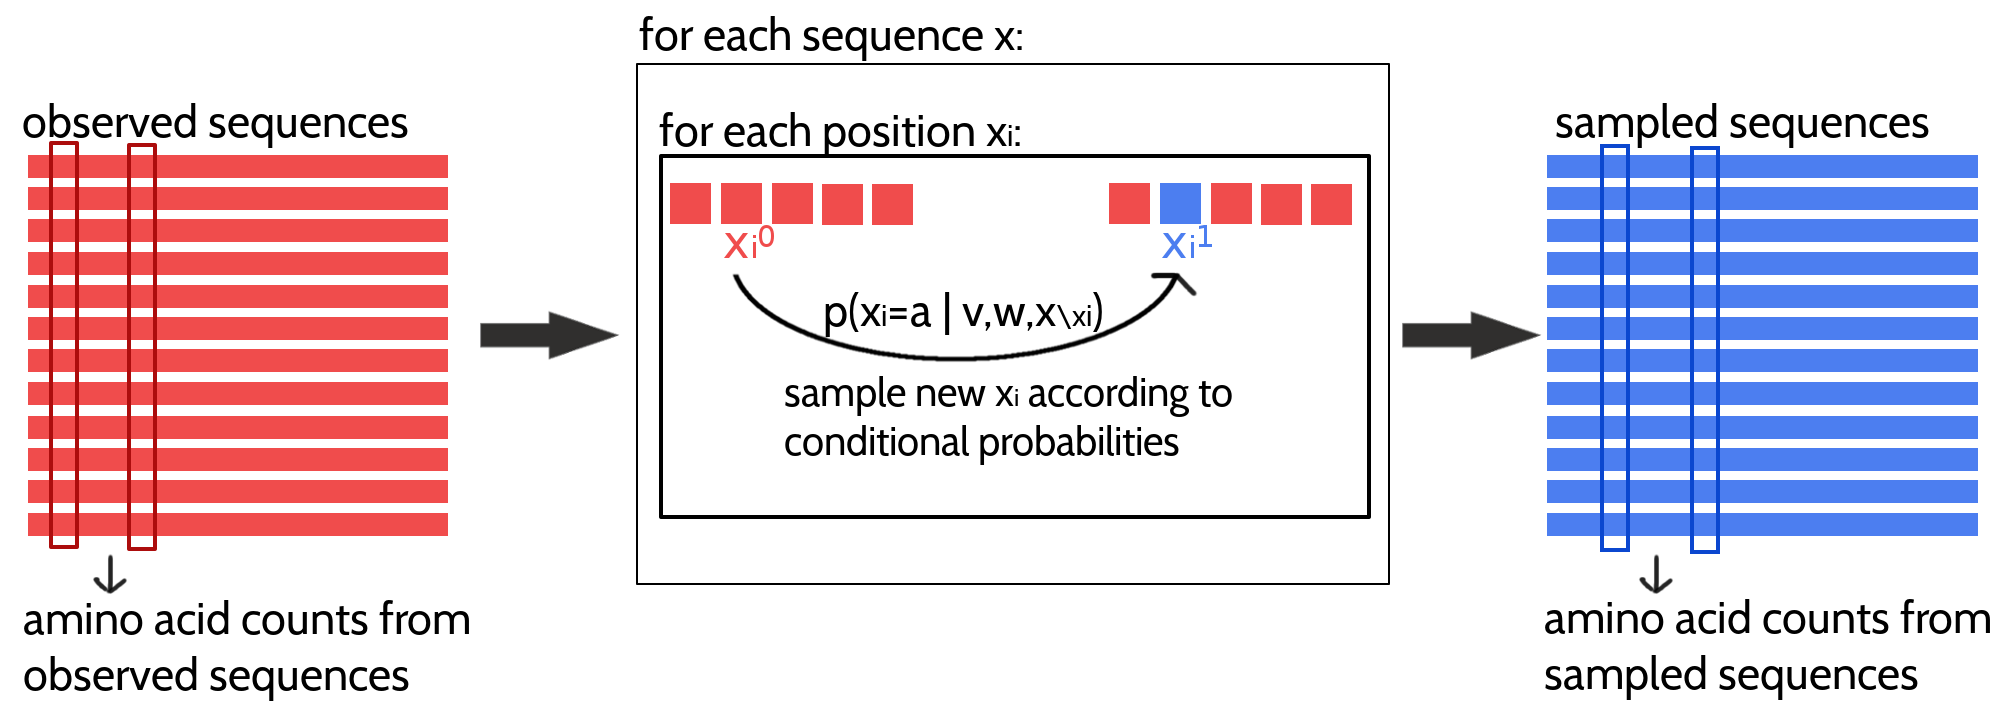
\includegraphics[width=0.9\linewidth]{img/full_likelihood/gibbs_sampling} 

}

\caption{Approximating the full likelihood gradient
of the \emph{Potts} model with \protect\hyperlink{abbrev}{CD}. Pairwise
amino acid counts are computed from the observed sequences of the input
alignment shown in red on the left. Expected amino acid frequencies
according to the model distribution are computed from a sampled
alignment shown in blue on the right. The \protect\hyperlink{abbrev}{CD}
approximation of the likelihood gradient is obtained by computing the
difference in amino acid counts of the observed and sampled alignment. A
newly sampled sequence is obtained by evolving a Markov chain, that is
initialized with an observed sequence, for one full Gibbs step. The
Gibbs step involves updating every position in the sequence (unless it
is a gap) according to the conditional probabilities for the 20 amino
acids at this position.}\label{fig:cd-gibbs-sampling}
\end{figure}

The next sections elucidate the optimization of the \emph{Potts} model
full likelihood with \protect\hyperlink{abbrev}{CD} to obtain an
approximation to the gradient.

\section{Optimizing the Full
Likelihood}\label{full-likelihood-optimization}

Given the likelihood gradient estimates obtained with
\protect\hyperlink{abbrev}{CD}, the full negative log likelihood can now
be minimized using a gradient descent optimization algorithm. Gradient
descent algorithms are used to find the minimum of an objective function
with respect to its parametrization by iteratively updating the
parameters values in the opposite direction of the gradient of the
objective function with respect to these parameters. \emph{Stochastic}
gradient descent (\protect\hyperlink{abbrev}{SGD}) is a variant thereof
that uses a stochastic estimate of the gradient whose average over many
updates approaches the true gradient. The stochasticity is commonly
obtained by evaluating a random subsample of the data at each iteration.
For \protect\hyperlink{abbrev}{CD} stochasticity additionally arises
from the Gibbs sampling process in order to obtain a gradient estimate
in the first place.

As a consequence of stochasticity, the gradient estimates are noisy,
resulting in parameter updates with high variance and strong
fluctuations of the objective function. These fluctuations enable
stochastic gradient descent to escape local minima but also complicate
finding the exact minimum of the objective function. By slowly
decreasing the step size of the parameter updates at every iteration,
stochastic gradient descent most likely will converge to the global
minimum for convex objective functions
{[}\protect\hyperlink{ref-Ruder2017}{192}--\protect\hyperlink{ref-Bottou2010}{194}{]}.
However, choosing an optimal step size for parameter updates as well as
finding the optimal annealing schedule offers a challenge and needs
manual tuning
{[}\protect\hyperlink{ref-Schaul2013}{195},\protect\hyperlink{ref-Zeiler2012}{196}{]}.
If the step size is chosen too small, progress will be unnecessarily
slow, if it is chosen too large, the optimum will be overshot and can
cause the system to diverge (see Figure
\ref{fig:gd-learning-rate-intro}). Further complications arise from the
fact that different parameters often require different optimal step
sizes, because the magnitude of gradients might vary considerably for
different parameters, e.g.~because of sparse data.












\begin{figure}

{\centering 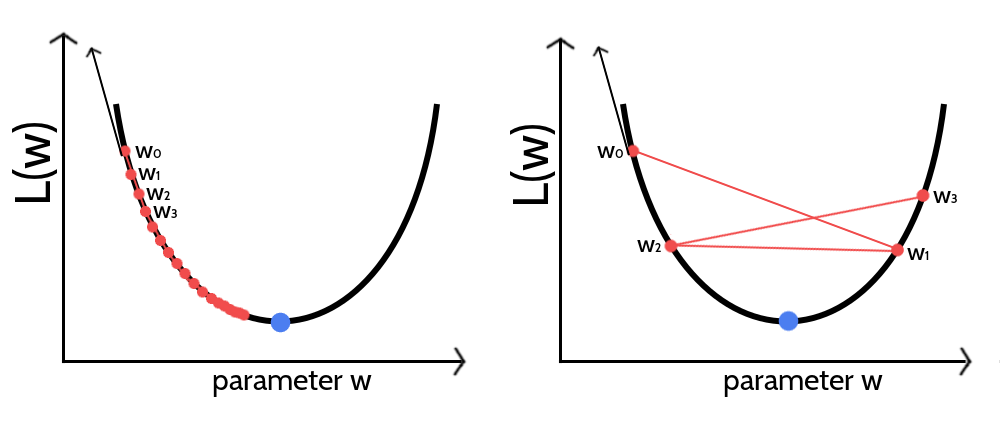
\includegraphics[width=0.8\linewidth]{img/full_likelihood/intro} 

}

\caption{Visualization of gradient descent
optimization of an objective function \(L(w)\) for different step sizes
\(\alpha\). The blue dot marks the minimum of the objective function.
The direction of the gradient at the initial parameter estimate \(w_0\)
is given as black arrow. The updated parameter estimate \(w_1\) is
obtained by taking a step of size \(\alpha\) into the opposite direction
of the gradient. \textbf{Left} If the step size is too small the
algorithm will require too many iterations to converge. \textbf{Right}
If the step size is too large, gradient descent will overshoot the
minimum and can cause the system to diverge.}\label{fig:gd-learning-rate-intro}
\end{figure}

Unfortunately, it is neither possible to use second order optimization
algorithms nor sophisticated first order algorithms like conjugate
gradients to optimize the full likelihood of the \emph{Potts} model.
While the former class of algorithms requires (approximate) computation
of the second partial derivatives, the latter requires evaluating the
objective function in order to identify the optimal step size via
linesearch, both being computationally too demanding.

The next subsections describe the hyperparameter tuning for stochastic
gradient descent, covering the choice of the convergence criterion and
finding the optimal learning rate annealing schedule.

\subsection{Convergence Criterion for Stochastic Gradient
Descent}\label{convergence-criteria-sgd}

In theory the gradient descent algorithm has converged and the optimum
of the objective function has been reached when the gradient becomes
zero. In practice the gradients will never be exactly zero, especially
due to the stochasticity of the gradient estimates when using stochastic
gradient descent with \protect\hyperlink{abbrev}{CD}. For this reason,
it is crucial to define a suitable convergence criterion that can be
tested during optimization and once the criterion is met, convergence is
assumed and the algorithm is stopped. Typically, the objective function
(or a related loss function) is periodically evaluated on a validation
set and the optimizer is halted whenever the function value saturates or
starts to increase. This technique is called early stopping and
additionally prevents overfitting
{[}\protect\hyperlink{ref-Bengio2012}{197},\protect\hyperlink{ref-Mahsereci2017}{198}{]}.
Unfortunately, we cannot compute the full likelihood function due to its
complexity and need to define a different convergence criterion.

One possibility is to stop learning when the L2 norm of the gradient for
the coupling parameters \(||\nabla_{\w} L\!L(\v^*, \w)||_2\) is close to
zero {[}\protect\hyperlink{ref-Carreira-Perpinan2005}{199}{]}. However,
when using a finite number of sequences for sampling, the norm of the
gradient does not converge to zero but towards a certain offset as it is
described in section \ref{cd-sampling-size}. Convergence could also be
monitored as the relative change of the norm of gradients within a
certain number of iterations. Optimization will be stopped when the
relative change becomes negligibly small, that is when the gradient norm
has reached a plateau. As gradient estimates are very noisy with
stochastic gradient descent, gradient fluctuations complicate the proper
assessment of this criterion.

Instead of the gradient, it is also possible to observe the relative
change of the norm of parameter estimates \(||\w||_2\) over several
iterations and stop learning when it falls below a small threshold
\(\epsilon\),

\begin{equation}
  \frac{||\w_{t-x}||_2 - ||\w_t||_2}{||\w_{t-x}||_2} < \epsilon \; .
  \label{eq:parameter-convergence-criterion}
\end{equation}

This measure is less noisy than subsequent gradient estimates because
the magnitude of parameter updates is bounded by the learning rate.

For stochastic gradient descent the optimum is a moving target and the
gradient will start oscillating when approaching the optimum. Therefore,
another idea is to monitor the direction of the partial derivatives.
However, this theoretical assumption is complicated by the fact that
gradient oscillations are also typically observed when the parameter
surface contains narrow valleys or generally when the learning rate is
too big, as it is visualized in the right plot in Figure
\ref{fig:gd-learning-rate-intro}. When optimizing high-dimensional
problems using the same learning rate for all dimensions, it is likely
that parameters converge at different speeds
{[}\protect\hyperlink{ref-Ruder2017}{192}{]} leading to oscillations
that could either originate from convergence or yet too large learning
rates. As can be seen in Figure \ref{fig:gradient-directions}, the
percentage of parameters for which the derivate changes direction within
the last \(x\) iterations is usually high and varies for different
proteins. Therefore it is not a good indicator of convergence. When
using the adaptive learning rate optimizer \emph{ADAM}, the momentum
term is an interfering factor for assessing the direction of partial
derivatives. Parameters will be updated into the direction of a smoothed
historical gradient and oscillations, regardless of which origin, will
be dampened. It is therefore hard to define a general convergence
criteria based on the direction of derivatives that can distinguish
these different scenarios.

















\begin{figure}

{\centering 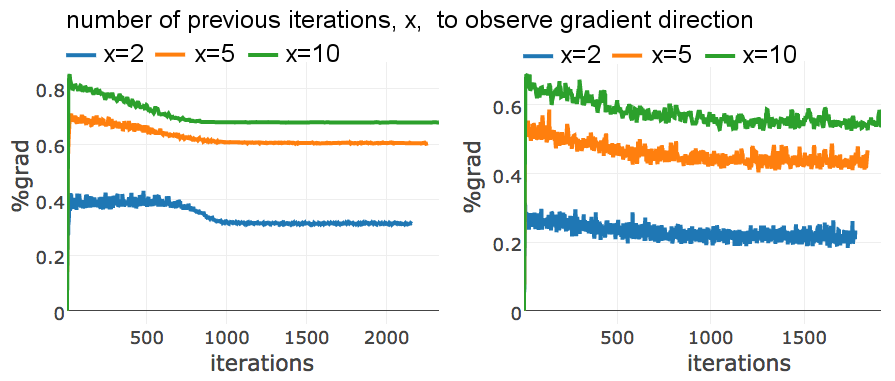
\includegraphics[width=1\linewidth]{img/full_likelihood/sgd/percentage_changes_in_gradient_direction_1c75A00_1ahoA00} 

}

\caption{Percentage of parameters for which the
derivate has changed its direction (i.e.~the sign) during the previous
\(x\) iterations (\(x\) is specified in the legend). Optimization is
performed with \protect\hyperlink{abbrev}{SGD} using the optimal
hyperparameters defined in section \ref{sgd-hyperparameter-tuning} and
using a regularization coefficient \(\lambda_w \eq 0.1L\) (see section
\ref{regularization-for-cd-with-sgd}) and using one step of Gibbs
sampling. Optimization is stopped when the relative change over the
L2-norm of parameter estimates \(||\w||_2\) over the last \(x\)
iterations falls below the threshold of \(\epsilon \eq 1e-8\).
Development has been monitored for two different proteins, \textbf{Left}
1c75A00 (protein length = 71, number sequences = 28078,
\protect\hyperlink{abbrev}{Neff} = 16808) \textbf{Right} 1ahoA00
(protein length = 64, number sequences = 378,
\protect\hyperlink{abbrev}{Neff} = 229).}\label{fig:gradient-directions}
\end{figure}

Of course, the simplest strategy to assume convergence is to specify a
maximum number of iterations for the optimization procedure, which also
ensures that the algorithm will stop eventually if none of the other
convergence criteria is met.

A necessary but not sufficient condition that is satisfied at the
optimum when the gradient is zero, is given by
\(\sum_{a,b=1}^{20} \wijab = 0\) (see section \ref{prior-v}). This
condition is never violated, as long as parameters satisfy this
criterion at initialization and the same step size is used to update all
parameters. To understand why, note that the 400 partial derivatives
\(\frac{\partial L\!L(\v^*, \w)}{\partial \wijab}\) for a residue pair
\((i,j)\) and for \(a,b \in \{1, \ldots, 20\}\) are not independent. The
sum over the 400 pairwise amino acid counts at positions \(i\) and \(j\)
is identical for the observed and the sampled alignment and amounts to,

\begin{equation}
  \sum_{a,b=1}^{20} N_{ij} q(x_i \eq a, q_j \eq b) = N_{ij} \; .
\end{equation}

Considering a residue pair \((i,j)\) and assuming amino acid pair
\((a,b)\) has higher counts in the sampled alignment than in the
observed input alignment, then this difference in counts must be
compensated by other amino acid pairs \((c,d)\) having less counts in
the sampled alignment compared to the true alignment (see Figure
\ref{fig:visualisation-wijab-constraint}). Therefore, it holds
\(\sum_{a,b=1}^{20} \frac{\partial L\!L(\v^*, \w)}{\partial \wijab} = 0\).
This symmetry is translated into parameter updates as long as the same
step size is used to update all parameters. However, when using adaptive
learning rates (e.g.~with the \emph{ADAM} optimizer), this symmetry is
broken and the condition \(\sum_{a,b=1}^{20} \wijab = 0\) can be
violated during the optimization processs. It is therefore interesting
to monitor \(\sum_{1 \le 1 < j \le L} \sum_{a,b=1}^{20} \wijab\).














\begin{figure}

{\centering 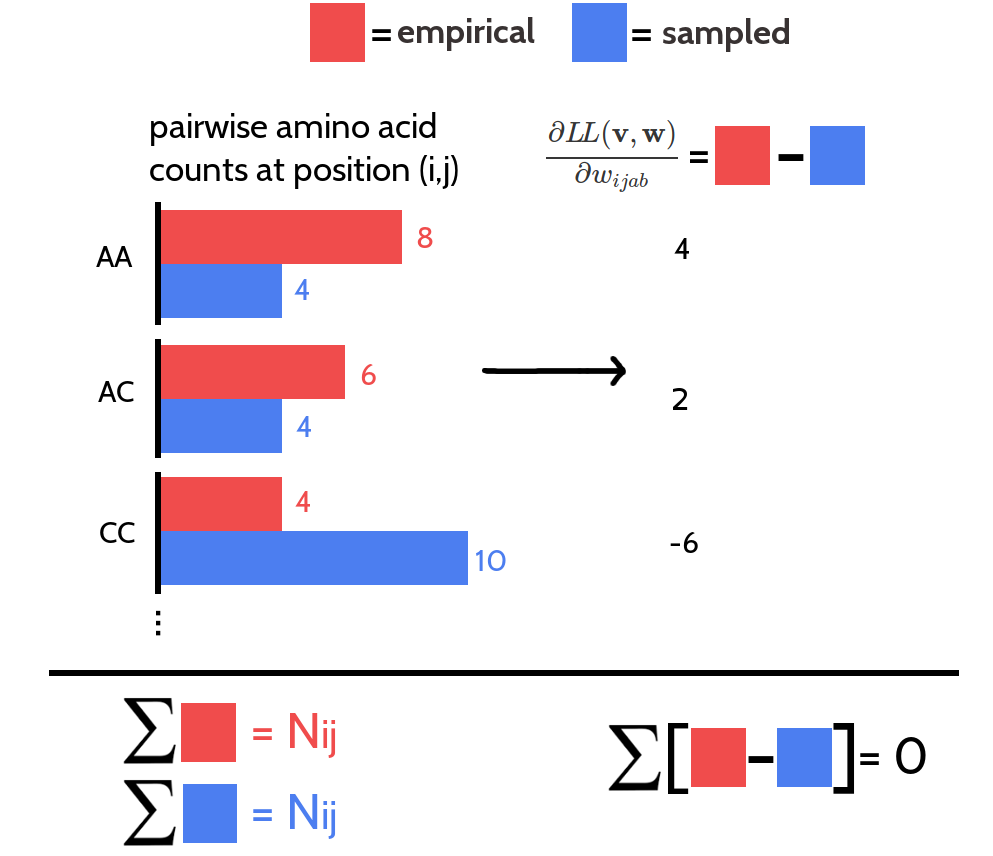
\includegraphics[width=0.6\linewidth]{img/full_likelihood/constraint_wijab} 

}

\caption{The 400 partial derivatives
\(\frac{\partial \LLreg(\v^*,\w)}{\partial \wijab}\) at position
\((i,j)\) for \(a,b \in \{1, \ldots, 20 \}\) are not independent. Red
bars represent pairwise amino acid counts at position \((i,j)\) for the
sampled alignment. Blue bars represent pairwise amino acid counts at
position \((i,j)\) for the input alignment. The sum over pairwise amino
acid counts at position \((i,j)\) for both alignments is \(N_{ij}\),
which is the number of ungapped sequences. The partial derivative for
\(\wijab\) is computed as the difference of pairwise amino acid counts
for amino acids \(a\) and \(b\) at position \((i,j)\). The sum over the
partial derivatives \(\frac{\partial \LLreg(\v^*,\w)}{\partial \wijab}\)
at position \((i,j)\) for all \(a,b \in \{1, \ldots, 20 \}\) is zero.}\label{fig:visualisation-wijab-constraint}
\end{figure}

\subsection{Tuning Hyperparameters of Stochastic Gradient Descent
Optimizer}\label{sgd-hyperparameter-tuning}

The coupling parameters \(\w\) will be updated at each time step \(t\)
by taking a step of size \(\alpha\) along the direction of the negative
gradient of the regularized full log likelihood,
\(- \nabla_w \LLreg(\v^*,\w)\), that has been approximated with
\protect\hyperlink{abbrev}{CD},

\begin{equation}
  \w_{t+1} = \w_t - \alpha \cdot \nabla_w \LLreg(\v^*,\w) \; .
\end{equation}

In order to get a first intuition of the optimization problem, I tested
initial learning rates
\(\alpha_0 \in \{1\mathrm{e}{-4}, 5\mathrm{e}{-4}, 1\mathrm{e}{-3}, 5\mathrm{e}{-3}\}\)
with a standard learning rate annealing schedule,
\(\alpha = \frac{\alpha_0}{1 + \gamma \cdot t}\) where \(t\) is the time
step and \(\gamma\) is the decay rate that is set to
0.01{[}\protect\hyperlink{ref-Bottou2012}{193}{]}.

Figure \ref{fig:performance-cd-alphaopt} shows the mean precision for
top ranked contacts computed from pseudo-likelihood couplings and from
\protect\hyperlink{abbrev}{CD} couplings optimized with stochastic
gradient descent using the four different learning rates. Overall, mean
precision for \protect\hyperlink{abbrev}{CD} contacts is lower than for
pseudo-likelihood contacts, especially when using the smallest
(\(\alpha_0 \eq 1\mathrm{e}{-4}\)) and largest
(\(\alpha_0 \eq 5\mathrm{e-}{3}\)) learning rate.









\begin{figure}

{\centering 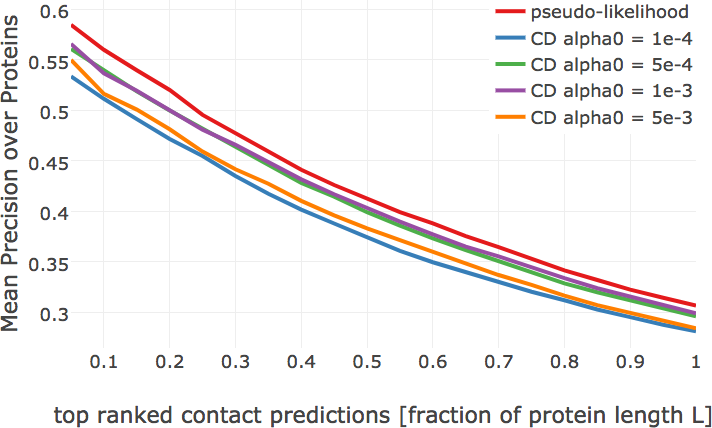
\includegraphics[width=0.85\linewidth]{img/full_likelihood/sgd/precision_vs_rank_learning_rates} 

}

\caption{Mean precision for top ranked
contact predictions over 300 proteins. Contact scores are computed as
the \protect\hyperlink{abbrev}{APC} corrected Frobenius norm of the
couplings \(\wij\). \textbf{pseudo-likelihood}: couplings computed with
pseudo-likelihood. \textbf{CD alpha0 = X}: couplings computed with
\protect\hyperlink{abbrev}{CD} using stochastic gradient descent with
different initial learning rates \(\alpha_0\) (see legend).}\label{fig:performance-cd-alphaopt}
\end{figure}

By looking at individual proteins it becomes evident that the optimal
learning rate depends on alignment size. Figure
\ref{fig:sgd-single-proteins-initial-learning-rate} displays the
development of the L2 norm of the coupling parameters, \(||\w||_2\),
during optimization using different learning rates for two proteins with
different alignment sizes. The left plot shows protein 1c75A00 that has
a large alignment with 28078 sequences (\protect\hyperlink{abbrev}{Neff}
= 16808) while the right plot shows protein 1ahoA00 that has a small
alignment with 378 sequences (\protect\hyperlink{abbrev}{Neff} = 229).
For protein 1ahoA00 and using a small initial learning rate
\(\alpha_0 \eq \mathrm{1e-4}\), the optimization runs very slowly and
does not converge within tha maximum number of 5000 iterations. Using a
large initial learning rate \(\alpha_0 \eq \mathrm{5e-3}\) results in
slighly overshooting the optimum at the beginning of the optimization
but with the learning rate decaying over time the parameter estimates
converge. In contrast, for protein 1c75A00, the choice of learning rate
has a more pronounced effect. With a small initial learning rate
\(\alpha_0 \eq \mathrm{1e-4}\) the optimization runs slowly but almost
converges within 5000 iterations. A large initial learning rate
\(\alpha_0 \eq \mathrm{5e-3}\) lets the parameters diverge quickly and
the optimum cannot be recovered. With learning rates
\(\alpha_0 \eq \mathrm{5e-4}\) and \(\alpha_0 \eq \mathrm{1e-3}\), the
optimum is well overshot at the beginning of the optimization but the
parameter estimates eventually converge as the learning rate decreases
over time.

These observations can be explained by the fact that the magnitude of
the gradient scales with the number of sequences in the alignment. The
gradient is computed from amino acid counts as explained before.
Therefore, alignments with many sequences will generally produce larger
gradients than alignments with few sequences, especially at the
beginning of the optimization procedure when the difference in amino
acid counts between sampled and observed sequences is largest. Following
these observations, I defined the initial learning rate \(\alpha_0\) as
a function of \protect\hyperlink{abbrev}{Neff},

\begin{equation}
  \alpha_0 = \frac{5\mathrm{e}{-2}}{\sqrt{N_{\text{eff}}}} \; .
  \label{eq:learning-rate-wrt-neff}
\end{equation}

For small \protect\hyperlink{abbrev}{Neff}, e.g.~5th percentile of the
distribution in the dataset \(\approx 50\), this definition of the
learning rate yields \(\alpha_0 \approx 7\mathrm{e}{-3}\) and for large
\protect\hyperlink{abbrev}{Neff}, e.g.~95th percentile
\(\approx 15000\), this yields \(\alpha_0 \approx 4\mathrm{e}{-4}\).
These values for \(\alpha_0\) lie in the optimal range that has been
observed for the two representative proteins in Figure
\ref{fig:performance-cd-alphaopt}. With the initial learning rate
defined as a function of \protect\hyperlink{bbrev}{Neff}, precision
slightly improves over the previous fixed learning rates (see Appendix
Figure \ref{fig:performance-cd-alphaopt-0}). All following analyses are
conducted using the \protect\hyperlink{abbrev}{Neff}-dependent initial
learning rate.














\begin{figure}

{\centering 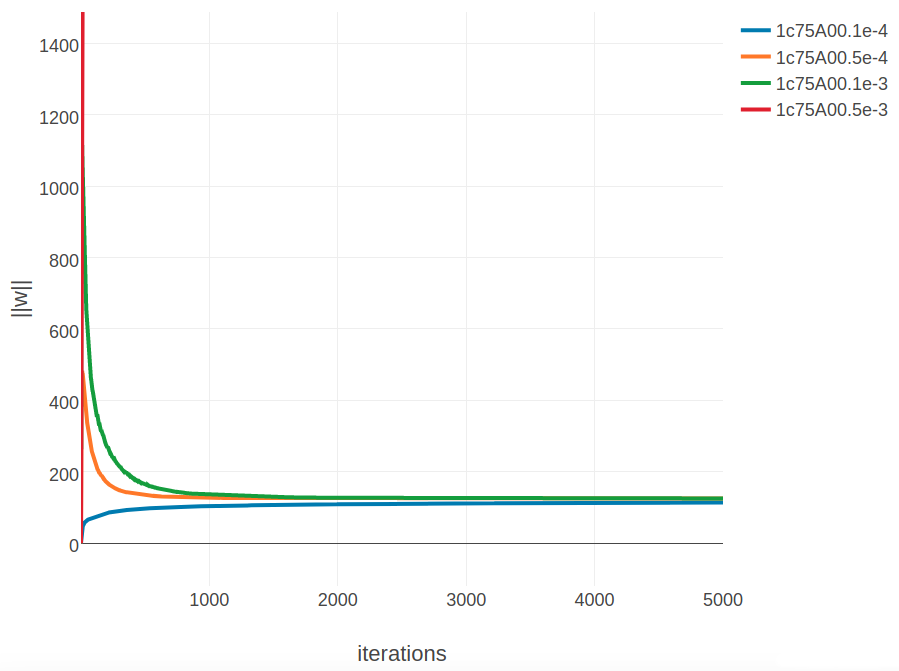
\includegraphics[width=0.48\linewidth]{img/full_likelihood/sgd/parameter_norm_1c75a00_alphas_lindecay001} 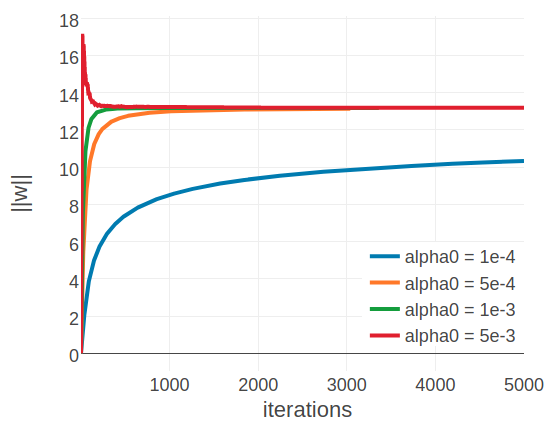
\includegraphics[width=0.48\linewidth]{img/full_likelihood/sgd/parameter_norm_1ahoa00_alphas_lindecay001} 

}

\caption{Convergence
plots for two proteins during \protect\hyperlink{abbrev}{SGD}
optimization with different learning rates and convergence measured as
L2-norm of the coupling parameters \(||\w||_2\). Linear learning rate
annealing schedule has been used with decay rate \(\gamma=0.01\) and
initial learning rates \(\alpha_0\) have been set as specified in the
legend. \textbf{Left} 1c75A00 (protein length = 71, number sequences =
28078, \protect\hyperlink{abbrev}{Neff} = 16808). Figure is cut at the
yaxis at \(||\w||_2=1000\), but learning rate of \(5\mathrm{e}{-3}\)
reaches \(||\w||_2 \approx 9000\). \textbf{Right} 1ahoA00 (protein
length = 64, number sequences = 378, \protect\hyperlink{abbrev}{Neff} =
229)}\label{fig:sgd-single-proteins-initial-learning-rate}
\end{figure}

In a next step, I evaluated the following learning rate annealing
schedules and decay rates using the
\protect\hyperlink{abbrev}{Neff}-dependent initial learning rate given
in eq. \eqref{eq:learning-rate-wrt-neff}:

\begin{itemize}
\tightlist
\item
  default linear learning rate schedule
  \(\alpha = \frac{\alpha_0}{1 + \gamma t}\) with
  \(\gamma \in \{1\mathrm{e}{-3}, 1\mathrm{e}{-2}, 1\mathrm{e}{-1}, 1 \}\)
\item
  square root learning rate schedule
  \(\alpha = \frac{\alpha_0}{\sqrt{1 + \gamma t}}\) with
  \(\gamma \in \{1\mathrm{e}{-2}, 1\mathrm{e}{-1}, 1 \}\)
\item
  sigmoidal learning rate schedule
  \(\alpha_{t+1} = \frac{\alpha_{t}}{1 + \gamma t}\) with
  \(\gamma \in \{1\mathrm{e}{-6}, 1\mathrm{e}{-5}, 1\mathrm{e}{-4}, 1\mathrm{e}{-3}\}\)
\item
  exponential learning rate schedule
  \(\alpha_{t+1} = \alpha_0 \cdot\exp(- \gamma t)\) with
  \(\gamma \in \{5\mathrm{e}{-4}, 1\mathrm{e}{-4}, 5\mathrm{e}{-3}\}\)
\end{itemize}

The learning rate annealing schedules are visualized for different decay
rates in Appendix Figure \ref{fig:learning-rate-schedules}. Optimizing
\protect\hyperlink{abbrev}{CD} with \protect\hyperlink{abbrev}{SGD}
using any of the learning rate schedules listed above yields on average
lower precision for the top ranked contacts than the pseudo-likelihood
contact score. Several learning rate schedules perform almost equally
and yield a mean precision that is about one to two percentage below the
mean precision for the pseudo-likelihood contact score (see Figure
\ref{fig:performance-cd-learnignrate-schedules}): a linear learning rate
schedule with decay rate \(\gamma \eq 1\mathrm{e}{-2}\), a sigmoidal
learning rate schedule with decay rates \(\gamma \eq 1\mathrm{e}{-5}\)
or \(\gamma \eq 1\mathrm{e}{-6}\) and an exponential learning rate
schedule with decay rates \(\gamma \eq 1\mathrm{e}{-3}\) or
\(\gamma \eq 1\mathrm{e}{-5}\). The square root learning rate schedule
gives ovarall bad results and does not lead to convergence because the
learning rate decays slowly at later time steps. The benchmark plots for
all learning rate schedules are shown in Appendix section
\ref{benchmark-learning-rate-annealing-schedules}.











\begin{figure}

{\centering 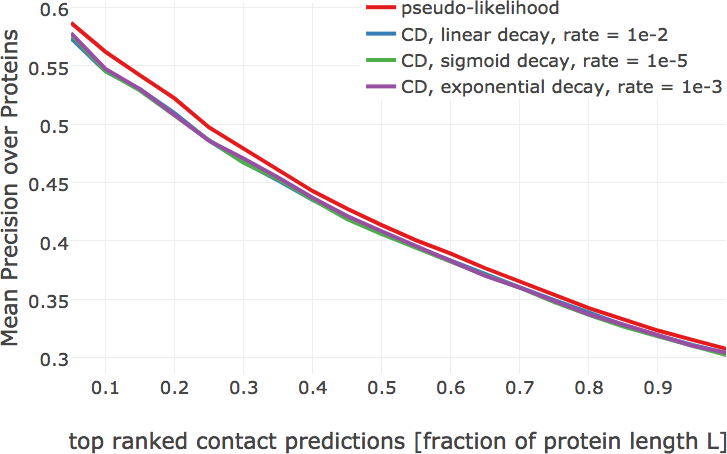
\includegraphics[width=0.9\linewidth]{img/full_likelihood/sgd/precision_vs_rank_schedules} 

}

\caption{Mean precision for
top ranked contact predictions over 300 proteins. Contact scores are
computed as the \protect\hyperlink{abbrev}{APC} corrected Frobenius norm
of the couplings \(\wij\). \textbf{pseudo-likelihood}: couplings
computed with pseudo-likelihood. \textbf{CD}: couplings computed with
\protect\hyperlink{abbrev}{CD} using stochastic gradient descent with an
initial learning rate defined with respect to
\protect\hyperlink{abbrev}{Neff}. Learning rate annealing schedules and
decay rates are specified in the legend.}\label{fig:performance-cd-learnignrate-schedules}
\end{figure}

In contrast to the findings regarding the initial learning rate earlier,
an optimal decay rate can be defined independent of the alignment size.
Figure \ref{fig:sgd-single-proteins-learning-rate-schedule} shows the
development of the L2 norm of the coupling parameters, \(||\w||_2\),
during optimization for the same two representative proteins with small
and large alignments as before. Convergence for protein 1ahoA00, having
small \protect\hyperlink{abbrev}{Neff}=229, is robust against the
particular choice of learning rate schedule and decay rate and the
presumed optimum at \(||w||_2 \approx 13.2\) is reached regardless of
the learning rate annealing schedule (see right plot in Figure
\ref{fig:sgd-single-proteins-learning-rate-schedule}). For protein
1c75A00, with high \protect\hyperlink{abbrev}{Neff}=16808, the choice of
the learning rate schedule has a notable impact on the rate of
convergence. Using a linear schedule, the learning rate decays quickly
but then converges to a certain offset, which effectively prevents
further optimization progress and the presumed optimum at
\(||w||_2 \approx 90\) is not reached within 5000 iterations. Learning
rate schedules that decay slower but decay continously for 5000
iterations, such as an exponential schedule with
\(\gamma \eq 1\mathrm{e}{-3}\) or a sigmoidal schedule with
\(\gamma \eq 1\mathrm{e}{-6}\), guide the parameter estimates close to
the expected optimum. Therefore, learning rate schedules with an
exponential or sigmoidal decay can be used with proteins having low
\protect\hyperlink{abbrev}{Neffs} as well as high
\protect\hyperlink{abbrev}{Neffs}.












\begin{figure}

{\centering 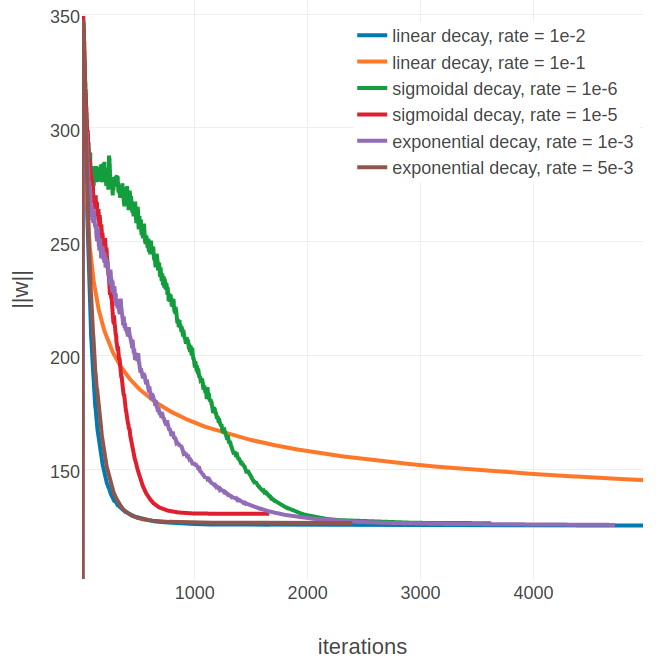
\includegraphics[width=0.48\linewidth]{img/full_likelihood/sgd/parameter_norm_1c75a00_alpha0_different_schedules} 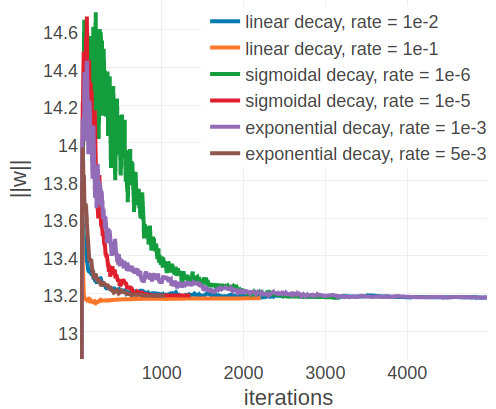
\includegraphics[width=0.48\linewidth]{img/full_likelihood/sgd/parameter_norm_1ahoa00_alpha0_different_schedules} 

}

\caption{L2-norm of the
coupling parameters \(||\w||_2\) during stochastic gradient descent
optimization with different learning rates schedules. The initial
learning rate \(\alpha_0\) is defined with respect to
\protect\hyperlink{abbrev}{Neff} as given in eq.
\eqref{eq:learning-rate-wrt-neff}. Learning rate schedules and decay rates
are used according to the legend. \textbf{Left} 1c75A00 (protein length
= 71, number sequences = 28078, \protect\hyperlink{abbrev}{Neff} =
16808). \textbf{Right} 1ahoA00 (protein length = 64, number sequences =
378, \protect\hyperlink{abbrev}{Neff} = 229)}\label{fig:sgd-single-proteins-learning-rate-schedule}
\end{figure}

Another aspect worth considering is runtime and it can be observed that
the different learning rate annealing schedules differ in convergence
speed. Figure \ref{fig:distribution-num-iterations} shows the
distribution over the number of iterations until convergence for
\protect\hyperlink{abbrev}{SGD} optimizations with five different
learning rate schedules that yield similar performance. The optimization
converges on average within less than 2000 iterations only when using
either a sigmoidal learning rate annealing schedule with decay rate
\(\gamma \eq 1\mathrm{e}{-5}\) or an exponential learning rate annealing
schedule with decay rate \(\gamma \eq 5\mathrm{e}{-3}\), On the
contrary, the distribution of iterations until convergence has a median
of 5000 when using a linear learning rate annealing schedule with
\(\gamma \eq 1\mathrm{e}{-2}\) or an exponential schedule with decay
rate \(\gamma \eq 1\mathrm{e}{-3}\). Under these considerations, I chose
a sigmoidal learning rate schedule with \(\gamma \eq 5\mathrm{e}{-6}\)
for all further analysis.












\begin{figure}

{\centering 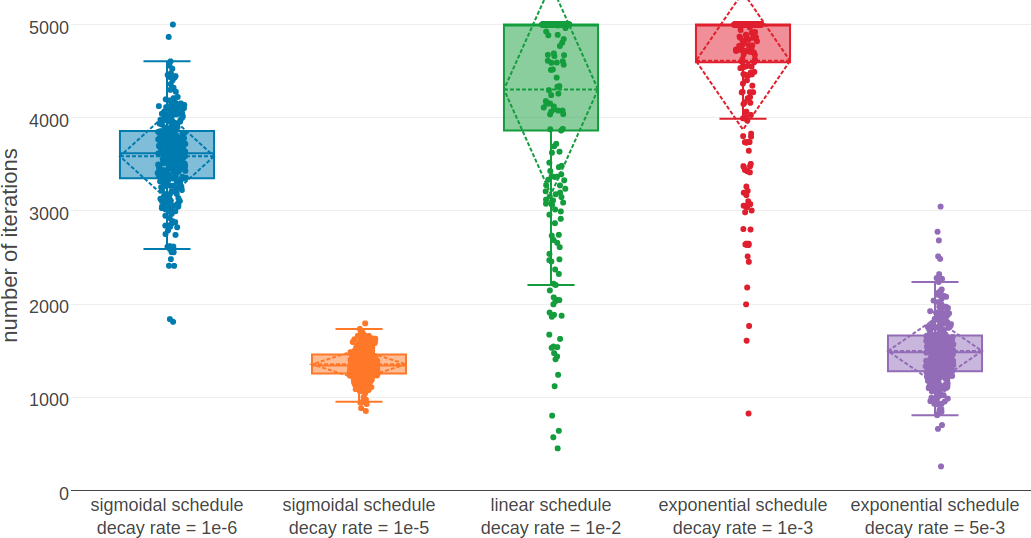
\includegraphics[width=1\linewidth]{img/full_likelihood/sgd/distribution_numiterations_against_selected_learningrate_schedules} 

}

\caption{Distribution of the number of
iterations until convergence for \protect\hyperlink{abbrev}{SGD}
optimizations of \protect\hyperlink{abbrev}{CD} for different learning
rate schedules. Convergence is reached when the relative difference of
parameter norms, \(||\w||_2\), over the last five iterations falls below
\(\epsilon \eq 1e-8\). Initial learning rate \(\alpha_0\) is defined
with respect to \protect\hyperlink{abbrev}{Neff} as given in eq.
\eqref{eq:learning-rate-wrt-neff} and maximum number of iterations is set
to 5000. Learning rate schedules and decay rates are specified in the
legend.}\label{fig:distribution-num-iterations}
\end{figure}

Finally, I checked whether altering the convergence criteria has notable
impact on performance. Per default, optimization is stopped whenever the
relative change of the L2 norm over coupling parameters, \(||\w||_2\),
over the last 5 iterations falls below a small value \(\epsilon < 1e-8\)
as denoted in eq. \eqref{eq:parameter-convergence-criterion}. Figure
\ref{fig:performance-cd-convergence-prev} shows that the mean precision
over proteins is robust to different settings of the number of
iterations over which the relative change is computed. The convergence
rate is mildly affected by the different settings. Optimization
converges on average within 1697, 1782 and 1917 iterations, when
computing the relative change of the parameter norm over the previous
2,5 and 10 iterations, respectively (see Appendix Figure
\ref{fig:numit-convergence-convergence-prev}). For all following
analysis, I chose 10 to be the number of iterations over which the
convergence criterion is computed.















\begin{figure}

{\centering 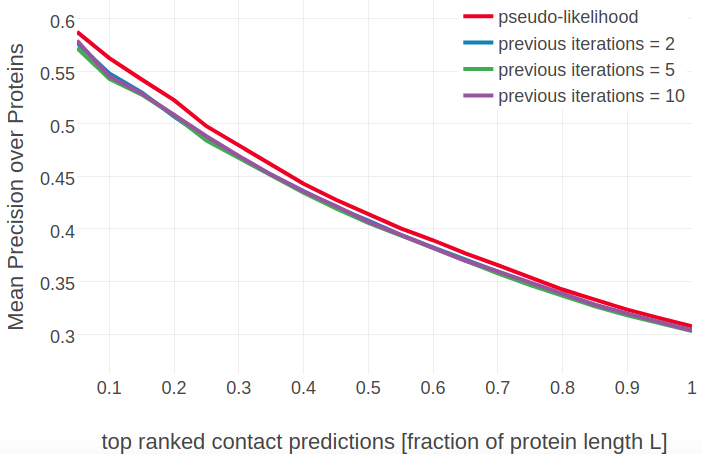
\includegraphics[width=0.9\linewidth]{img/full_likelihood/sgd/precision_vs_rank_convergence_prev} 

}

\caption{Mean precision for top
ranked contact predictions over 300 proteins. Contact scores are
computed as the \protect\hyperlink{abbrev}{APC} corrected Frobenius norm
of the couplings \(\wij\). \textbf{pseudo-likelihood}: couplings
computed with pseudo-likelihood. \textbf{\#previous iterations = X}:
couplings computed with \protect\hyperlink{abbrev}{CD} using stochastic
gradient descent with an initial learning rate defined with respect to
\protect\hyperlink{abbrev}{Neff} and the sigmoidal learning rate
schedule with \(\gamma \eq 5\mathrm{e}{-6}\). The relative change of the
L2 norm over coupling parameters, \(||\w||_2\), is evaluated over the
previous X iterations (specified in the legend) and convergence is
assumed when the relative change falls below a small value
\(\epsilon \eq 1e-8\).}\label{fig:performance-cd-convergence-prev}
\end{figure}

\section{Tuning the Gibbs Sampling Scheme for Contrastive
Divergence}\label{cd-sampling-optimization}

The original \protect\hyperlink{abbrev}{CD}-k algorithm described by
Hinton in 2002 evolves the Markov chains by k=1 Gibbs steps
{[}\protect\hyperlink{ref-Hinton2002}{188}{]}. As described earlier,
\protect\hyperlink{abbrev}{CD}-1 provides a biased estimate of the true
gradient because the Markov chains have not reached the stationary
distribution {[}\protect\hyperlink{ref-Fischer2012}{190}{]}. Bengio and
Delalleau show that the bias for \protect\hyperlink{abbrev}{CD}-k kan be
understood as a residual term when expressing the log likelihood
gradient as an expansion that involves the k-th sample of the Gibbs
chain
{[}\protect\hyperlink{ref-Bengio2009}{191},\protect\hyperlink{ref-Ma2016}{200}{]}.
As the number of Gibbs steps, k, goes to infinity the residual term and
hence the bias converges to zero and the \protect\hyperlink{abbrev}{CD}
gradient estimate converges to a stochastic estimation of the true
likelihood gradient. Indeed, eventhough surprising results have been
obtained by evolving the Markov chains for only one Gibbs step,
typically \protect\hyperlink{abbrev}{CD}-k for
k\textgreater{}\textgreater{}1 gives more precise results
{[}\protect\hyperlink{ref-Bengio2009}{191}{]}. Furthermore it has been
shown, that bias also depends on the mixing rate (rate of convergence)
of the chains whereby the mixing rate decreases when model parameters
increase {[}\protect\hyperlink{ref-Tieleman2008}{201}{]}. This can lead
to divergence of the \protect\hyperlink{abbrev}{CD}-k solution from
optimal solution in a sense that the model systematically gets worse as
optimization progresses {[}\protect\hyperlink{ref-Fischer2010}{202}{]}.
Regularization of the parameters offers a solution to this problem,
constraining the magnitude of the parameters. A different solution
suggested by Bengio and Delalleau is to dynamically increase k when the
model parameters increase {[}\protect\hyperlink{ref-Bengio2009}{191}{]}.
These studies analysing the convergence properties and the expected
approximation error for \protect\hyperlink{abbrev}{CD}-k have mainly
been conducted for Restricted Boltzmann Machines. It is therefore not
clear, whether and to what extent these findings apply to the
\emph{Potts} model.

Several connections of \protect\hyperlink{abbrev}{CD} to other well
known approximation algorithms have been drawn. For example, it can be
shown that \protect\hyperlink{abbrev}{CD} using one Gibbs update step on
a randomly selected variable is exactly equivalent to a stochastic
maximum pseudo-likelihood estimation
{[}\protect\hyperlink{ref-Hyvarinen2006}{203},\protect\hyperlink{ref-Hyvarinen2007}{204}{]}.
Asuncion and colleagues showed further that an arbitrary good
approximation to the full likelihood can be reached by applying
blocked-Gibbs sampling {[}\protect\hyperlink{ref-Asuncion2010}{205}{]}.
\protect\hyperlink{abbrev}{CD} based on sampling an arbitraty number of
variables, has an equivalent stochastic composite likelihood, which is a
higher-order generalization of the pseudo-likelihood.

Another variant of \protect\hyperlink{abbrev}{CD} is
\protect\hyperlink{abbrev}{PCD}, such that the Markov chain is not
reinitialized at a data sample every time a new gradient is computed
{[}\protect\hyperlink{ref-Tieleman2008}{201}{]}. Instead, the Markov
chains are kept \emph{persistent} that is, they are evolved between
successive gradient computations. The fundamental idea behind
\protect\hyperlink{abbrev}{PCD} is that the model changes only slowly
between parameter updates given a sufficiently small learning rate.
Consequently, the Markov chains will not be pushed too far from
equilibrium after each update but rather stay close to the stationary
distribution
{[}\protect\hyperlink{ref-Murphy2012}{94},\protect\hyperlink{ref-Fischer2012}{190},\protect\hyperlink{ref-Tieleman2008}{201}{]}.
Tieleman and others observed that \protect\hyperlink{abbrev}{PCD}
performs better than \protect\hyperlink{abbrev}{CD} in all practical
cases tested, eventhough \protect\hyperlink{abbrev}{CD} can be faster in
the early stages of learning and thus should be preferred when runtime
is the limiting factor
{[}\protect\hyperlink{ref-Murphy2012}{94},\protect\hyperlink{ref-Tieleman2008}{201},\protect\hyperlink{ref-Swersky2010}{206}{]}.

The next sections discuss various modifications of the
\protect\hyperlink{abbrev}{CD} algorithm, such as varying the
regularization strength \(\lambda_w\) for constraining the coupling
parameters \(\w\), increasing the number of Gibbs sampling steps and
varying the number of Markov chains used for sampling. Persistent
contrastive divergence is analysed for various combinations of the above
mentioned settings and eventually combined with
\protect\hyperlink{abbrev}{CD}-k. Unless noted otherwise, all
optimizations will be performed using stochastic gradient descent with
the tuned hyperparameters described in the last sections.

\subsection{Tuning Regularization Coefficients for Contrastive
Divergence}\label{regularization-for-cd-with-sgd}

For tuning the hyperparameters of the stochastic gradient descent
optimizer in the last section \ref{sgd-hyperparameter-tuning}, the
coupling parameters \(\w\) were constrained by a Gaussian prior
\(\mathcal{N}(\w | 0, \lambda_w^{-1} I)\) using the default
pseudo-likelihood regularization coefficient
\(\lambda_w \eq 1\mathrm{e}{-2}L\) as decscribed in methods section
\ref{methods-regularization}. It is conceivable that
\protect\hyperlink{abbrev}{CD} achieves optimal performance using
stronger or weaker regularization than used for pseudo-likelihood
optimization. Therefore, I evaluated performance for different
regularization coefficients
\(\lambda_w \in \{ 5\mathrm{e}{-2}L, 1\mathrm{e}{-1}L, 1\mathrm{e}{-2}L, L\}\)
using the previously identified hyperparamters for
\protect\hyperlink{abbrev}{SGD}. The single potentials \(\v\) are not
subject to optimization and are kept fixed at their maximum-likelihood
estimate \(v^*\) that is derived in eq. \eqref{eq:prior-v}.

As can be seen in Figure \ref{fig:precison-cd-regularization}, using
strong regularization for the couplings, with \(\lambda_w \eq L\),
results in a drastic drop of mean precision. Using weaker
regularization, with \(\lambda_w \eq \mathrm{5e}{-2}L\), improves
precision for the top \(L/10\) and \(L/5\) predicted contacts but
decreases precision when including lower ranked predictions. As a matter
of fact, a slightly weaker regularization
\(\lambda_w \eq \mathrm{1e}{-1}L\) than the default
\(\lambda_w \eq \mathrm{1e}{-2}L\) improves mean precision especially
for the top \(L/2\) contacts in such a way, that it is comparable to the
pseudo-likelihood performance.












\begin{figure}

{\centering 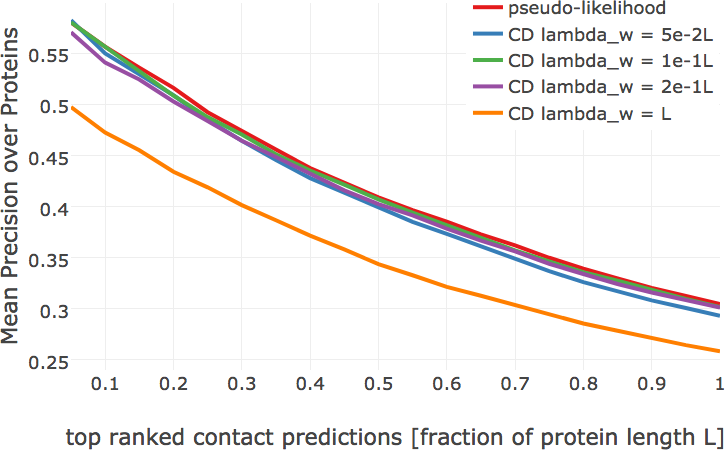
\includegraphics[width=0.9\linewidth]{img/full_likelihood/sgd/precision_vs_rank_regularizer} 

}

\caption{Mean precision for top ranked
contact predictions over 300 proteins. Contact scores are computed as
the \protect\hyperlink{abbrev}{APC} corrected Frobenius norm of the
couplings \(\wij\). \textbf{pseudo-likelihood}: couplings computed with
pseudo-likelihood. \textbf{CD lambda\_w = X}: couplings computed with
\protect\hyperlink{abbrev}{CD} using L2-regularization on the couplings
\(\w\) with regularization coefficient \(\lambda_w\) specified in the
legend and keeping the single potentials \(\vi\) fixed at their
\protect\hyperlink{abbrev}{MLE} optimum \(\vi^*\) denoted in eq.
\eqref{eq:prior-v}.}\label{fig:precison-cd-regularization}
\end{figure}

As mentioned before, in contrast to pseudo-likelihood optimization the
single potentials \(\v\) are not optimized with
\protect\hyperlink{abbrev}{CD} but rather set to their
maximum-likelihood estimate as it is obtained in a single position model
that is discussed in methods section \eqref{eq:prior-v}. When the single
potentials \(\v\) are optimized with \protect\hyperlink{abbrev}{CD}
using the same regularization coefficient \(\lambda_v \eq 10\) as for
pseudo-likelihood optimization, performance is almost indistinguishable
compared to keeping the single potentials \(\v\) fixed (see Appendix
Figure \ref{fig:full-likelihood-opt-fixv}).

\subsection{Varying the Sample Size}\label{cd-sampling-size}

The default Gibbs sampling scheme outlined in method section
\ref{methods-cd-sampling} involves the random selection of \(10L\)
sequences from the input alignment, with \(L\) being protein length, at
every iteration of the optimization procedure. These selected sequences
are used to initialize the same number of Markov chains. The particular
choice of \(10L\) sequences was motivated by the fact that there is a
relationship between the precision of contacts predicted from
pseudo-likelihood and protein length, at least for alignments with less
than \(10^3\) diverse sequences
{[}\protect\hyperlink{ref-Anishchenko2017}{174}{]}. It has been argued
that roughly \(5L\) nonredundant sequences are required to obtain
confident predictions that can bet used for protein structure prediction
{[}\protect\hyperlink{ref-Kamisetty2013}{102}{]}.

I analysed whether varying the number of sequences used for the
approximation of the gradient via Gibbs sampling affects performance.
Randomly selecting only a subset of sequences \(S\) from the \(N\)
sequences of the input alignment corresponds to the stochastic gradient
descent idea of a minibatch and introduces additional stochasticity over
the \protect\hyperlink{abbrev}{CD} Gibbs sampling process. Using
\(S < N\) sequences for Gibbs sampling has the further advantage of
decreasing the runtime at each iteration. I evaluated different schemes
for the random selection of sequences:

\begin{itemize}
\tightlist
\item
  sampling \(x\)L sequences with \(x \in \{ 1, 5, 10, 50 \}\) without
  replacement enforcing \(S \eq \min(N, xL)\)
\item
  sampling \(x\)\protect\hyperlink{abbrev}{Neff} sequences with
  \(x \in \{ 0.2, 0.3, 0.4 \}\) without replacement
\end{itemize}

Figure \ref{fig:cd-performance-samplesize} illustrates performance for
several of the choices. Randomly selecting \(L\) sequences for sampling
results in a visible drop in performance. There is no benefit in using
more than \(10L\) sequences, especially as sampling more sequences
increases runtime per iteration. Specifying the number of sequences for
sampling as fractions of \protect\hyperlink{abbrev}{Neff} generally
improves precision slightly over selecting \(10L\) or \(50L\) sequences
for sampling. By sampling \(0.3\)\protect\hyperlink{abbrev}{Neff}
sequences, \protect\hyperlink{abbrev}{CD} does slighty improve over
pseudo-likelihood.














\begin{figure}

{\centering 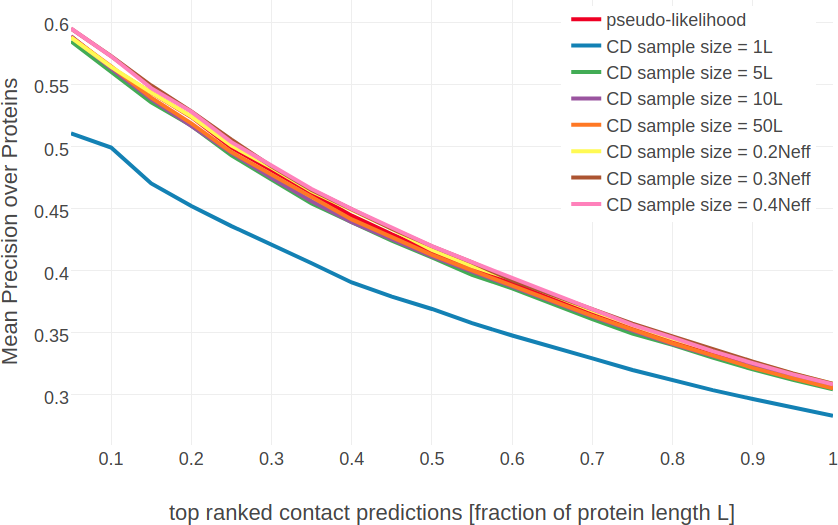
\includegraphics[width=0.9\linewidth]{img/full_likelihood/gibbs_sampling/precision_vs_rank_samplesize} 

}

\caption{Mean precision for top ranked
contact predictions over 300 proteins. Contact scores are computed as
the \protect\hyperlink{abbrev}{APC} corrected Frobenius norm of the
couplings \(\wij\). \textbf{pseudo-likelihood}: couplings computed with
pseudo-likelihood. \textbf{CD sample size = X }: contact scores computed
from \protect\hyperlink{abbrev}{CD} with
\protect\hyperlink{abbrev}{SGD}. At every iteration, a particular number
of sequences is randomly selected from the input alignmet to initialize
the Markoc chains for Gibbs sampling. The number of randomly selected
sequences is specified in the legend. It is defined either as multiples
of protein length \(L\) or as fraction of the effective number of
sequences \protect\hyperlink{abbrev}{Neff}.}\label{fig:cd-performance-samplesize}
\end{figure}

When evaluating performance with respect to the number of effective
sequences \protect\hyperlink{abbrev}{Neff}, it can clearly be noted that
the optimal number of randomly selected sequences should be defined as a
fraction of \protect\hyperlink{abbrev}{Neff}. Selecting too many
sequences, e.g. \(50L\) for small alignments (left plot in Figure
\ref{fig:cd-precision-sampling-size-neff}), or selecting too few
sequences, e.g \(1L\) for large alignments (right plot in Figure
\ref{fig:cd-precision-sampling-size-neff}), results in a decrease in
precision compared to defining the number of sequences as fractions of
\protect\hyperlink{abbrev}{Neff}. Especially small alignments benefit
from sample sizes defined as a fraction of
\protect\hyperlink{abbrev}{Neff} with improvements of about three
percentage points in precision over pseudo-likelihood.

















\begin{figure}

{\centering 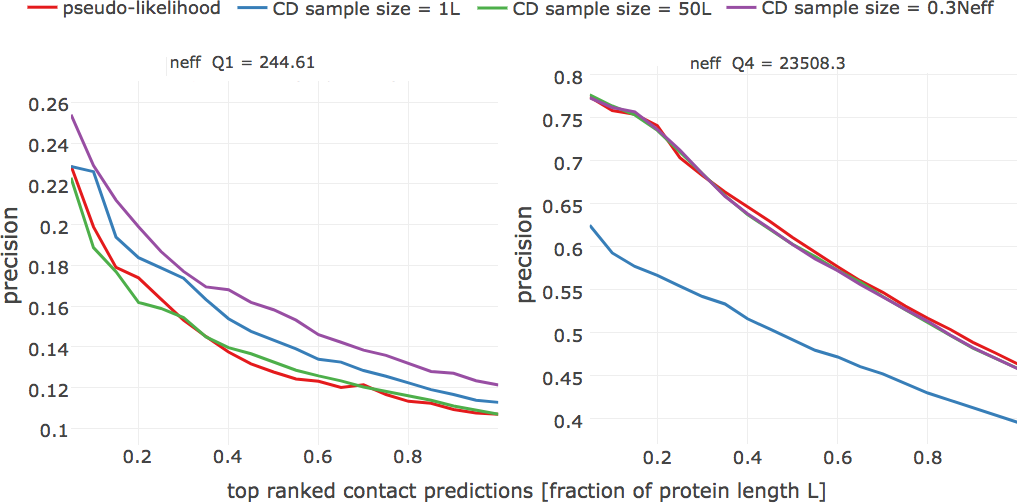
\includegraphics[width=1\linewidth]{img/full_likelihood/gibbs_sampling/precision_vs_rank_facetted_by_neff_samplesize} 

}

\caption{Mean precision for top
ranked contact predictions over subsets of 75 proteins, defined
according to \protect\hyperlink{abbrev}{Neff} quartiles. Contact scores
are computed as the \protect\hyperlink{abbrev}{APC} corrected Frobenius
norm of the couplings \(\wij\). \textbf{pseudo-likelihood}: contact
scores computed from pseudo-likelihood. \textbf{CD sample size = X }:
contact scores computed from \protect\hyperlink{abbrev}{CD} with
\protect\hyperlink{abbrev}{SGD}. The number of randomly selected
sequences for the Gibbs sampling process is specified in the legend. It
is defined either as multiples of protein length \(L\) or as fraction of
the effective number of sequences \protect\hyperlink{abbrev}{Neff}.
\textbf{Left} Subset of 75 proteins with
\protect\hyperlink{abbrev}{Neff} \textless{} Q1. \textbf{Right} Subset
of 75 proteins with Q3 \textless{}= \protect\hyperlink{abbrev}{Neff}
\textless{} Q4.}\label{fig:cd-precision-sampling-size-neff}
\end{figure}

To understand the effect of different choices of sample size it is
necessary to look at single proteins. The left plot in Figure
\ref{fig:cd-samplesize-protein1c75a00} shows the development of the L2
norm of the gradient for couplings,
\(||\nabla_{\w} L\!L(\v^*, \w)||_2\), for protein chain 1c75A00 that is
of length 71 and has \protect\hyperlink{abbrev}{Neff} = 16808. The norm
of the gradient decreases during optimization and for increasing choices
of the sample size it saturates at decreasing levels. For example,
increasing the sample size by a factor 100 (from \(L\) to \(100L\))
leads to an approximately 10-fold reduction of the norm of the gradient
at convergence (\(\mathrm{1e}{+5}\) compared to \(\mathrm{1e}{+4}\)),
which corresponds to a typical reduction of statistical noise as the
square root of the number of samples. It is not feasible to sample the
number of sequences at each iteration that would be necessary to reduce
the norm of the gradient to near zero!

The previous benchmark showed, that precision of the top ranked contacts
does not improve to the same amount as the norm of the gradient
decreases when the sample size is increased. Probably, the improved
gradient when using a larger sample size helps to finetune the
parameters, which only has a negligible effect on the contact score
computed as \protect\hyperlink{abbrev}{APC} corrected Frobenius norm of
the couplings \(\wij\). For example, the difference between the
parameter norm at convergence for sampling \(10L = 710\) sequences or
\(50L = 3550\) sequences is only marginal (see right plot in Figure
\ref{fig:cd-samplesize-protein1c75a00}), despite a larger difference of
the norm of gradients.

It is not clear why an improved gradient estimate due to sampling more
sequences results in weaker performance for proteins with small
alignments as could be seen in the previous benchmark in Figure
\ref{fig:cd-precision-sampling-size-neff}. Protein 1ahoA00, that has
length 64 and an alignment of 378 sequences
(\protect\hyperlink{abbrev}{Neff}=229), achieves a mean precision of
0.44 over the top \(0.1L\) - \(L\) contacts when using all \(N \eq 378\)
sequences for sampling. When only \(0.3N_{\textrm{eff}} \eq 69\)
sequences are used in the sampling procedure, 1ahoA00 achieves a mean
precision of 0.62. Appendix Figure
\ref{fig:cd-samplesize-protein1ahoa00} shows the course of the norm of
the gradient and the norm of coupling parameters during optimization for
this protein. Similarly as it has been observed for protein 1c75A00, the
norm of the gradient converges towards smaller values when more
sequences are used in the Gibbs sampling process and the improved
gradient is supposed to lead to a better approximation of the
likelihood. One explanation for this obvious discrepancy could be some
effect of overfitting. Eventhough a regularizer is used for optimization
and the norm of coupling parameters actually is smaller when using a
larger sample size (see the right plot in Appendix Figure
\ref{fig:cd-samplesize-protein1ahoa00}).














\begin{figure}

{\centering 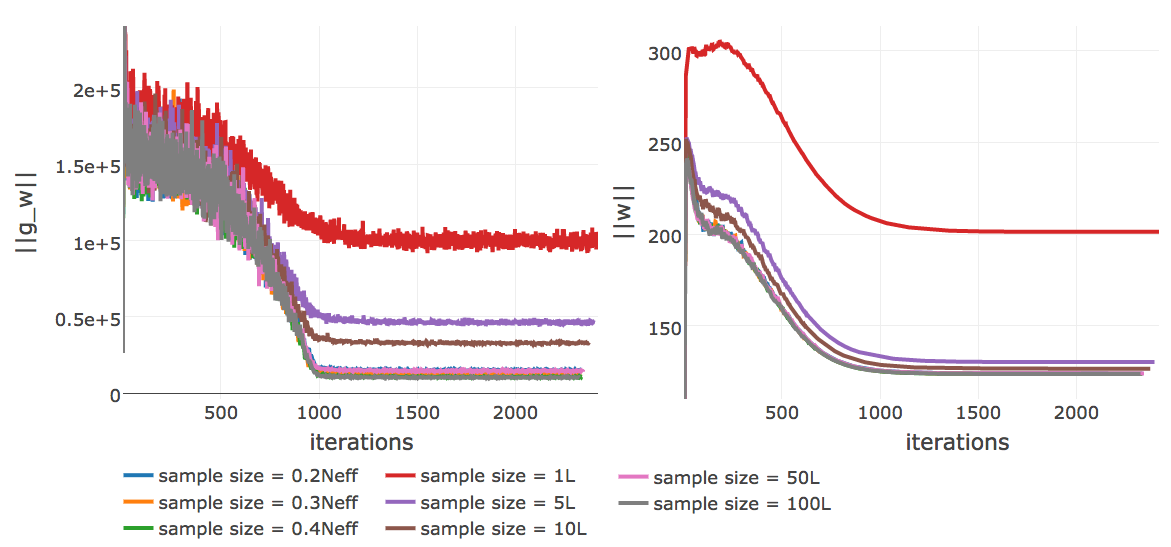
\includegraphics[width=1\linewidth]{img/full_likelihood/gibbs_sampling/1c75A00_gradient_and_parameter_norm_for_samplesizes} 

}

\caption{Monitoring parameter norm and
gradient norm for protein 1c75A00 during \protect\hyperlink{abbrev}{SGD}
using different sample sizes. Protein 1c75A00 has length L=71 and 28078
sequences in the alignment (\protect\hyperlink{abbrev}{Neff}=16808). The
number of sequences, that is used for Gibbs sampling to approximate the
gradient, is given in the legend with 1L = 71 sequences, 5L = 355
sequences, 10L = 710 sequences, 50L = 3550 sequences, 100L = 7100
sequences, 0.2Neff = 3362 sequences, 0.3Neff = 5042 sequences, 0.4Neff =
6723 sequences. \textbf{Left} L2-norm of the gradients for coupling
parameters, \(||\nabla_{\w} L\!L(\v^*, \w)||_2\) (without contribution
of regularizer). \textbf{Right} L2-norm of the coupling parameters
\(||\w||_2\).}\label{fig:cd-samplesize-protein1c75a00}
\end{figure}

\subsection{Varying the number of Gibbs Steps}\label{cd-gibbs-steps}

As discussed earlier, it has been pointed out in the literature that
using \(k>1\) Gibbs steps for sampling sequences gives more precise
results at the cost of longer runtimes per gradient evaluation
{[}\protect\hyperlink{ref-Bengio2009}{191},\protect\hyperlink{ref-Tieleman2008}{201}{]}.
I analysed the impact on performance when the number of Gibbs steps is
increased to 5 and 10. As can be seen in Figure
\ref{fig:precision-cd-gibbs-steps}, increasing the number of Gibbs steps
does result in a slight drop of performance. When evaluating precision
with respect to \protect\hyperlink{abbrev}{Neff} it can be found that
using more Gibbs sampling steps is especially disadvantageous for large
alignments (see Appendix Figure \ref{fig:cd-precision-gibbssteps-neff}).










\begin{figure}

{\centering 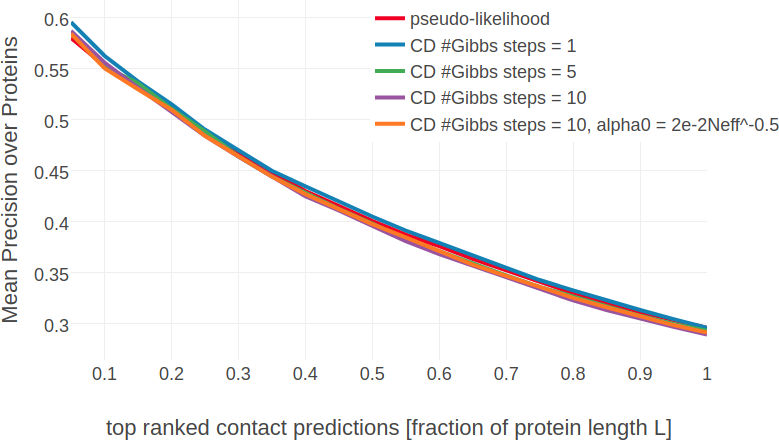
\includegraphics[width=0.9\linewidth]{img/full_likelihood/gibbs_sampling/precision_vs_rank_gibbssteps} 

}

\caption{Mean precision for top ranked
contact predictions over 300 proteins. Contact scores are computed as
the \protect\hyperlink{abbrev}{APC} corrected Frobenius norm of the
couplings \(\wij\). \textbf{pseudo-likelihood}: contact scores computed
from pseudo-likelihood. \textbf{CD \#Gibbs steps = X}: contact scores
computed from \protect\hyperlink{abbrev}{CD} optimized with
\protect\hyperlink{abbrev}{SGD} and evolving each Markov chain using the
number of Gibbs steps specified in the legend.}\label{fig:precision-cd-gibbs-steps}
\end{figure}

When evaluating single proteins, it can be observed that for proteins
with small alignments the L2 norm of the parameters, \(||\w||_2\),
converges towards a different offset when using more than one Gibbs
steps (see left plot in Figure \ref{fig:cd-gibbssteps-single-proteins}).
Naturally, the Markov chains can wander further away from their
initialization when they are evolved over a longer time which results in
a stronger gradient at the beginning of the optimization. Therefore and
because the initial learning rate has been optimized for sampling with
one Gibbs step, the parameter norm overshoots the optimum at the
beginning. Even when lowering the initial learning rate from
\(\alpha_0 = \frac{5e-2}{\sqrt{N_{\text{eff}}}}\) to
\(\alpha_0 \in \left \{ \frac{3e-2}{\sqrt{N_{\text{eff}}}}, \frac{2e-2}{\sqrt{N_{\text{eff}}}} , \frac{1e-2}{\sqrt{N_{\text{eff}}}} \right \}\),
the \protect\hyperlink{abbrev}{SGD} optimizer evidently approaches a
different optimum. Surprisingly, the different optimum that is found for
proteins with small alignments has no substantial impact on precision,
as becomes evident from Figure \ref{fig:cd-precision-gibbssteps-neff}.
For proteins with large alignments it can be observed that there is not
one alternative solution to the parameters, but depending on the number
of Gibbs steps and on the initial learning rate, \(\alpha_0\), the L2
norm over parameters converges towards various different offsets (see
right plot in Figure \ref{fig:cd-gibbssteps-single-proteins}). It is not
clear how these observations can be interpreted, in particular given the
fact, that the L2 norm of gradients,
\(||\nabla_{\w} L\!L(\v^*, \w)||_2\), converges to the identical offset
for all settings regardless of alignment size (see Appendix Figure
\ref{fig:cd-gibbssteps-single-proteins-gradient}). Optimizing
\protect\hyperlink{abbrev}{CD} with 10 Gibbs steps and using a smaller
initial learning rate, \(\alpha0 = \frac{2e-2}{\sqrt{N_{\text{eff}}}}\),
does not have an overal impact on mean precision as can be seen in
Figure \ref{fig:precision-cd-gibbs-steps}.













\begin{figure}

{\centering 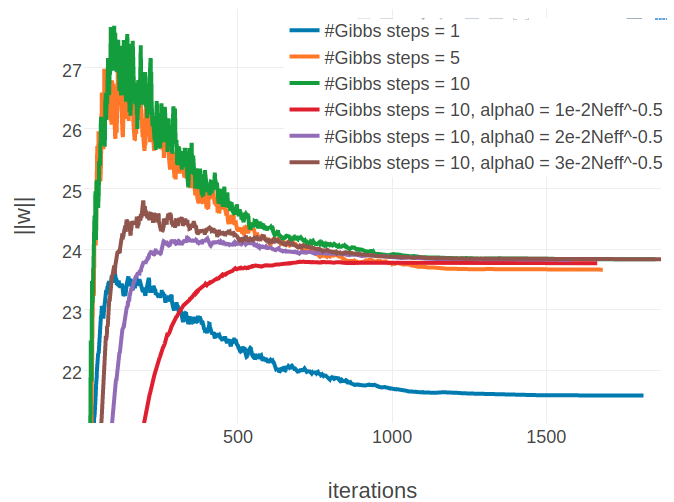
\includegraphics[width=0.48\linewidth]{img/full_likelihood/gibbs_sampling/parameter_norm_1ahoa00} 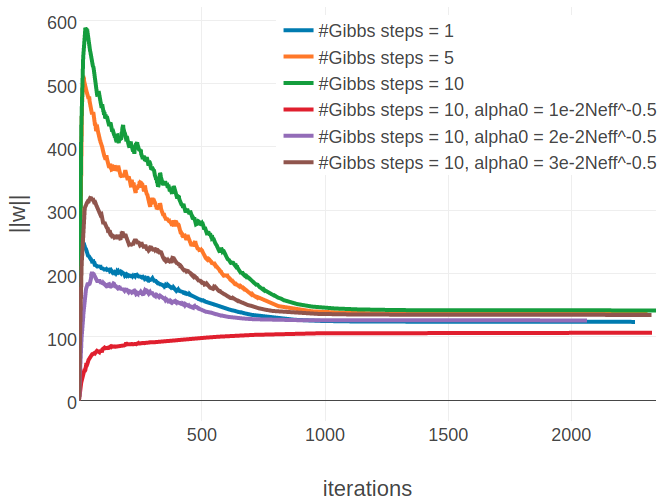
\includegraphics[width=0.48\linewidth]{img/full_likelihood/gibbs_sampling/parameter_norm_1c75a00} 

}

\caption{Monitoring parameter norm,
\(||\w||_2\), for protein 1aho\_A\_00 and 1c75\_A\_00 during
\protect\hyperlink{abbrev}{SGD} optimization using different number of
Gibbs steps and initial learning rates, \(\alpha_0\). Number of Gibbs
steps is given in the legend, as well as particular choices for the
initial learning rate, when not using the default
\(\alpha_0 = \frac{5e-2}{\sqrt{N_{\text{eff}}}}\). \textbf{Left} Protein
1aho\_A\_00 has length L=64 and 378 sequences in the alignment
(\protect\hyperlink{abbrev}{Neff}=229) \textbf{Right} Protein
1c75\_A\_00 has length L=71 and 28078 sequences in the alignment
(\protect\hyperlink{abbrev}{Neff}=16808).}\label{fig:cd-gibbssteps-single-proteins}
\end{figure}

\subsection{Persistent Contrastive Divergence}\label{cd-gibbs-steps}

Finally I analysed, whether evolving the Markov chains over successive
iterations, which is known as \protect\hyperlink{abbrev}{PCD}, does
improve performance {[}\protect\hyperlink{ref-Tieleman2008}{201}{]}.
Several empirical studies have shown that
\protect\hyperlink{abbrev}{PCD} performs superior compared to
\protect\hyperlink{abbrev}{CD}-1 and also to
\protect\hyperlink{abbrev}{CD}-10
{[}\protect\hyperlink{ref-Tieleman2008}{201},\protect\hyperlink{ref-Swersky2010}{206}{]}.
In the literatur is has been pointed out that
\protect\hyperlink{abbrev}{PCD} needs to use small learning rates
because in order to sample from a distribution close to the stationary
distribution, the parameters cannot change too rapidly. However, using
smaller learning rates not only increases runtime but also requires
tuning of the learning rate and learning rate schedule once again. Since
it has been found, that \protect\hyperlink{abbrev}{CD} is faster in
learning at the beginning of the optimization, I tested a compromise,
that uses \protect\hyperlink{abbrev}{CD}-1 at the beginning of the
optimization and when learning slows down,
\protect\hyperlink{abbrev}{PCD} is switched on. Concretely,
\protect\hyperlink{abbrev}{PCD} is switched on, when the relative change
of the norm of coupling parameters, \(||\w||_2\), falls below
\(\epsilon \in \{\mathrm{1e}{-3}, \mathrm{1e}{-5}\}\) while the
convergence criterion is not altered and convergence is assumed when the
relative change falls below \(\epsilon \eq \mathrm{1e}{-8}\). As a
result, the model will already have approached the optimum when
\protect\hyperlink{abbrev}{PCD} is switched on so that the coupling
parameters \(\w\) will mot change to quickly over many updates.



















\begin{figure}

{\centering 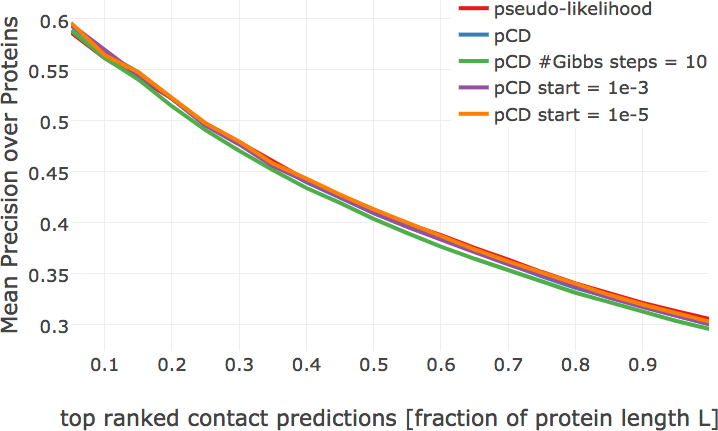
\includegraphics[width=0.9\linewidth]{img/full_likelihood/pcd/precision_vs_rank_notitle} 

}

\caption{Mean precision for top ranked contact
predictions over 300 proteins. Contact scores are computed as the
\protect\hyperlink{abbrev}{APC} corrected Frobenius norm of the
couplings \(\wij\). \textbf{pseudo-likelihood}: contact scores computed
from pseudo-likelihood. \textbf{pCD}: contact scores computed from
\protect\hyperlink{abbrev}{PCD} optimized with
\protect\hyperlink{abbrev}{SGD} using the hyperparameters that have been
found to work optimal with \protect\hyperlink{abbrev}{CD} as described
throughout the last sections. \textbf{pCD \#Gibbs steps = 10}: same as
pCD, but evolving the Gibbs chain for 10 steps. \textbf{pCD start =
1e-3}: \protect\hyperlink{abbrev}{SGD} optimization starts by optimizing
the full likelihood using the \protect\hyperlink{abbrev}{CD} gradient
approximation and switches to the \protect\hyperlink{abbrev}{PCD}
gradient approximation once the relative change of L2 norm of parameters
has fallen below \(\epsilon \eq \mathrm{1e}{-3}\) evaluated over the
last 10 iterations. \textbf{pCD start = 1e-5}: same as `pCD start =
1e-3', but with \(\epsilon \eq \mathrm{1e}{-5}\).}\label{fig:precision-pcd}
\end{figure}

Figure \ref{fig:precision-pcd} shows the mean precision of top ranked
contacts on the validation set computed with several
\protect\hyperlink{abbrev}{PCD} variants that perform almost equally
well. Evolving the Gibbs chains for k=10 steps results in a slight drop
in performance, just as it has been observed for
\protect\hyperlink{abbrev}{CD}. Optimizing the full likelihoood with
\protect\hyperlink{abbrev}{CD} and switiching to
\protect\hyperlink{abbrev}{PCD} at a later stage of optimization does
also not have a notable impact on performance.

Again it is insightful to observe the optimization progresss for single
proteins. For protein 1ahoA00, with low
\protect\hyperlink{abbrev}{Neff}=229, the
\protect\hyperlink{abbrev}{PCD} model converges to the same coupling
norm offset (\(||\w||_2 \approx 24\)) as the
\protect\hyperlink{abbrev}{CD} model using 5 and 10 Gibbs steps (see
left plot in Figure \ref{fig:pcd-single-proteins} compared to left plot
in \ref{fig:cd-gibbssteps-single-proteins}). It can also be seen that
when \protect\hyperlink{abbrev}{PCD} is switched on at a later stage of
optimization the coupling norm jumps from the
\protect\hyperlink{abbrev}{CD}-1 level to the
\protect\hyperlink{abbrev}{PCD} level. The different optimum that is
found for proteins with small alignments does not seem to affect
predictive performance. Interestingly, convergence behaves differently
for protein 1c75A00, that has high
\protect\hyperlink{abbrev}{Neff}=16808 (see right plot in Figure
\ref{fig:pcd-single-proteins}). \protect\hyperlink{abbrev}{PCD} using
one Gibbs step converges to a different coupling norm offset than
\protect\hyperlink{abbrev}{CD}-1 and \protect\hyperlink{abbrev}{PCD}
using ten Gibbs steps. However, when \protect\hyperlink{abbrev}{PCD} is
switched on later during optimization the model either ends up in the
\protect\hyperlink{abbrev}{CD}-1 (switch at \(\epsilon \eq 1e-5\) or
\(\epsilon \eq 1e-6\)) or in the \protect\hyperlink{abbrev}{PCD} optimum
(switch at \(\epsilon \eq 1e-3\)). The cause for this behaviour is
unclear, yet it has no noticable impact on overal performance.















\begin{figure}

{\centering 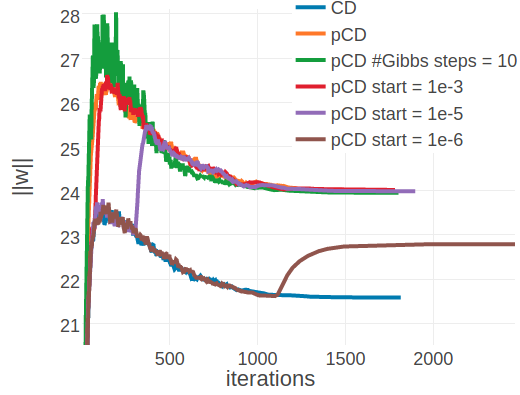
\includegraphics[width=0.48\linewidth]{img/full_likelihood/pcd/1ahoA00_parameter_norm} 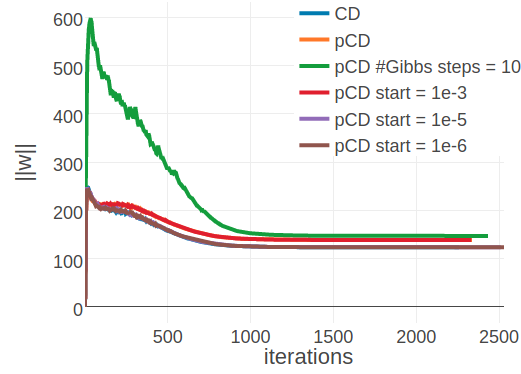
\includegraphics[width=0.48\linewidth]{img/full_likelihood/pcd/1c75A00_parameter_norm} 

}

\caption{Monitoring parameter norm,
\(||\w||_2\), for protein 1ahoA00 and 1c75A00 during
\protect\hyperlink{abbrev}{SGD} optimization of different objectives.
\textbf{Left} Protein 1ahoA00 has length L=64 and 378 sequences in the
alignment (\protect\hyperlink{abbrev}{Neff}=229) \textbf{Right} Protein
1c75A00 has length L=71 and 28078 sequences in the alignment
(\protect\hyperlink{abbrev}{Neff}=16808). \textbf{CD} contrastive
divergence using 1 Gibbs step. \textbf{pCD} persistent contrastive
divergence using 1 Gibbs step. \textbf{pCD \#Gibbs steps = 10}
persistent contrastive divergence using 10 Gibbs steps. \textbf{pCD
start = 1e-3}, \textbf{pCD start = 1e-5}: same as in Figure
\ref{fig:precision-pcd} \textbf{pCD start = 1e-6}: same as `pCD start =
1e-3', but with \(\epsilon \eq \mathrm{1e}{-6}\).}\label{fig:pcd-single-proteins}
\end{figure}

Against expectations from the findings in literature, neither
\protect\hyperlink{abbrev}{CD}-k with k\textgreater{}1 Gibbs steps nor
\protect\hyperlink{abbrev}{PCD} does improve performance with respect to
precision of the top ranked contact predictions. Swersky and colleagues
ellaborated on various choices of hyperparameters (e.g momentum,
averaging, regularization, etc.) for training Restricted Boltzmann
Machines as classifiers with \protect\hyperlink{abbrev}{CD}-k and
\protect\hyperlink{abbrev}{PCD}
{[}\protect\hyperlink{ref-Swersky2010}{206}{]}. They found many
subtleties that need to be explored and can play a crucial role for
successfull training. In section \ref{sgd-hyperparameter-tuning} I
manually tuned the learning rate and annealing schedule for stoachstic
gradient descent to be used with \protect\hyperlink{abbrev}{CD}-1. It is
plausible, that these settings are not optimal for
\protect\hyperlink{abbrev}{CD}-k with k\textgreater{}1 Gibbs steps and
\protect\hyperlink{abbrev}{PCD} and require tuning once again. Because
hyperparameter optimization with stochastic gradient descent is a
time-consuming task, in the following, I applied the popular \emph{ADAM}
stochastic gradient descent optimizer that does in theory not require
tuning many hyperparameters
{[}\protect\hyperlink{ref-Kingma2014}{207}{]}.

\section{Using ADAM to optimize Contrastive
Divergence}\label{adam-results}

\emph{ADAM} computes per-parameter adaptive learning rates and includes
momentum and the default values have been found to work quite well (see
methods section \ref{methods-full-likelihood-adam} for details)
{[}\protect\hyperlink{ref-Ruder2017}{192},\protect\hyperlink{ref-Kingma2014}{207}{]}.
However, I tested different learning rates for \emph{ADAM} to optimize
the full likelihood with \protect\hyperlink{abbrev}{CD}-1 for protein
1mkcA00 (number of sequences = 142) and 1c75A00 (number of sequences =
28078) and found that both proteins require a differnt optimal learning
rate. In contrast to plain stochastic gradient descent, with \emph{ADAM}
it is possible to use larger learning rates for proteins having large
alignments, because the learning rate will be adapted to the magnitude
of the gradient for every parameter individually. For protein 1mkcA00,
with \protect\hyperlink{abbrev}{Neff}=96, a learning rate of 5e-3
quickly leads to convergence whereas for protein 1c75A00, having
\protect\hyperlink{abbrev}{Neff}=16808, an even larger learning rate can
be chosen to obtain quick convergence (see Appendix Figure
\ref{fig:adam-learning-rate}). Therefore, I again specified the learning
rate as a function of \protect\hyperlink{abbrev}{Neff},

\begin{equation}
  \alpha = 2\mathrm{e}{-3}\log(\text{N}_{\text{eff}}) \; ,
  \label{eq:learning-rate-wrt-neff-adam}
\end{equation}

such that or small \protect\hyperlink{abbrev}{Neff}, e.g.~5th percentile
of the distribution in the dataset \(\approx 50\), this definition of
the learning rate yields \(\alpha_0 \approx 8\mathrm{e}{-3}\) and for
large \protect\hyperlink{abbrev}{Neff}, e.g.~95th percentile
\(\approx 15000\), this yields \(\alpha_0 \approx 2\mathrm{e}{-2}\).

It is interesting to note, that the norm of the coupling parameters,
\(||\w||_2\), converges towards different values depending on the choice
of the learning rate \(\alpha\) ((see Appendix Figure
\ref{fig:adam-learning-rate}). By default, \emph{ADAM} uses a constant
learning rate, because the algorithm performs a kind of step size
annealing by nature. However, popular implementations of \emph{ADAM} in
the
\href{https://github.com/fchollet/keras/blob/master/keras/optimizers.py\#L385}{Keras}
{[}\protect\hyperlink{ref-Chollet2015}{208}{]} and
\href{https://github.com/Lasagne/Lasagne/blob/master/lasagne/updates.py\#L565-L629}{Lasagne}
{[}\protect\hyperlink{ref-Dieleman2015}{209}{]} packages allow the use
of an annealing schedule. I therefore tested \emph{ADAM} with a
sigmoidal learning rate annealing schedule which already gave good
results for \protect\hyperlink{abbrev}{SGD} (see section
\ref{sgd-hyperparameter-tuning}). Indeed, as can be seen in Appendix
Figure \ref{fig:adam-learning-rate-annealing}, when \emph{ADAM} is used
with a sigmoidal decay of the learning rate, the L2-norm of the coupling
parameters \(||\w||_2\) converges roughly towards the same value. For
the following analysis I used \emph{ADAM} with a learning rate defined
as a function of \protect\hyperlink{abbrev}{Neff} and a sigmoidal
learning rate annealing schedule with decay rate \(\gamma \eq 5e-6\).

TODO

A problem when using \emph{ADAM} is that the necessarty condidtion
\(\sum_{a,b=1}^{20} \wijab = 0\) is violated (see section
\ref{convergence-criteria-sgd}).

\section{Comparing CD couplings to pLL
couplings}\label{comparing-pll-cd}

The previous sections dealed intensively with the hyperparameter
optimization for the stochastic gradient descent optimizer and the
\protect\hyperlink{abbrev}{CD} model itself. Eventhough the adaptive
learning rate optimizer \emph{ADAM} did not improve performance over
plain stochastic gradient descent, it is still likely that appropriate
modifications to the optimization procedure, e.g.~averaging
{[}\protect\hyperlink{ref-Ma2016}{200}{]}, might be beneficial for
particular variants of \protect\hyperlink{abbrev}{CD}. As dicussed in
section \ref{convergence-criteria-sgd}, the convergence criterion is a
crucial aspect for optimization, not only affecting runtime but also
preventing overfitting. It might be worth to assess the convergence
properties with more sophisticated convergence metrics, like the
EB-criterion proposed by Mahsereci et al.
{[}\protect\hyperlink{ref-Mahsereci2017}{198}{]}, instead of using the
L2 norm of the coupling parameters, \(||\w||_2\).

Against expectations, the best performance with respect to the precision
of the top ranked contacts, was obtained by using the most simple
variant of the \emph{contrastive divergence} algorithm,
\protect\hyperlink{abbrev}{CD}-1. With \protect\hyperlink{abbrev}{CD}-1,
sequence samples are generated according to the current state of the
model by evolving Gibbs chains, that have been initialized at data
samples, for only one full step. Interestingly, better gradient
estimates that were obtained by running more Gibbs chains in parallel
(see section \ref{cd-sampling-size}), did not carry over to better
predictive performance. It is possible that the improved gradient helps
to finetune the parameters which has no effect on the contact score,
computed as the \protect\hyperlink{abbrev}{APC} corrected Frobenius norm
of the couplings, and the ovaral ranking of residue pairs. Furthermore,
it can be speculated that the heuristic contact score that has
empirically been found to work very well for pseudo-likelihood
couplings, might not be an appropriate choice for couplings computed
with \protect\hyperlink{abbrev}{CD}.













\begin{figure}

{\centering 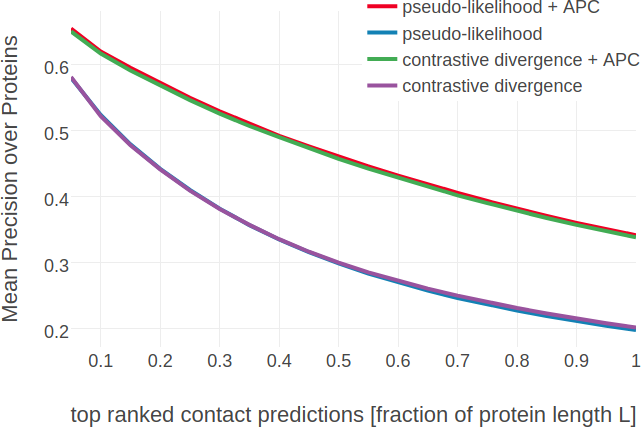
\includegraphics[width=0.9\linewidth]{img/full_likelihood/final/precision_vs_rank_notitle} 

}

\caption{Mean precision for top ranked contact
predictions over 2000 proteins. \textbf{pseudo-likelihood (APC)} Contact
score is computed as \protect\hyperlink{abbrev}{APC} corrected Frobenius
norm of the couplings computed from pseudo-likelihood.
\textbf{pseudo-likelihood} same as ``pseudo-likelihood (APC)'' but
without \protect\hyperlink{abbrev}{APC} \textbf{contrastive divergence
(APC)} Contact score is computed as \protect\hyperlink{abbrev}{APC}
corrected Frobenius norm of the couplings computed from
contrastive-divergence. \textbf{contrastive divergence} same as
``contrastive divergence (APC)'' but without
\protect\hyperlink{abbrev}{APC}.}\label{fig:precision-cd-final}
\end{figure}

A final benchmark over a larger set of proteins (2000 proteins randomly
selected from subsets 5 to 10 described in method section \ref{dataset})
reveals that contact predictions obtained by maximizing the
pseudo-likelihood and by optimizing the full likelihood with contrastive
divergence perform similar (see Figure \ref{fig:precision-cd-final}). At
any rate it is interesting to not only compare pseudo-likelihood and
contrastive divergence based on ovaral performance, but to also have a
look at single predictions. In the following, I will examine and compare
the predicitons made by both methods for two representative proteins,
one with a small alignment and low corresponding
\protect\hyperlink{abbrev}{Neff} value and one with a large alignment
and high corresponding \protect\hyperlink{abbrev}{Neff} value.

\subsection{Protein 1c75A00}\label{protein-1c75a00}

Protein 1c75A00 has length L=71 and 28078 sequences in the alignment and
is among the proteins with the highest number of effective sequences
(\protect\hyperlink{abbrev}{Neff}=16808 \textgreater{} 95th percentile).
The contact score (\protect\hyperlink{abbrev}{APC} corrected Frobenius
norm of the couplings \(\wij\)) computed from pseudo-likelihood and
contrastive divergence couplings performs equally well (see Appendix
Figure \ref{fig:precision-pll-cd-1c75a00}). The 14 (=L/5) highest
scoring contacts predicted with \protect\hyperlink{abbrev}{CD} are true
positive contacts according to an \(8 \angstrom \Cb\) distance cutoff
compared to 13 true positive contacts predicted with pseudo-likelihood.
Both methods predict very similar contact maps (see Figure
\ref{fig:contact-maps-1c75a00}). The highest scoring predictions (top
L/5 contacts marked with croses) are identical except for one contact,
which is the false positive contact predicted by the pseudo-likelihood.









\begin{figure}

{\centering 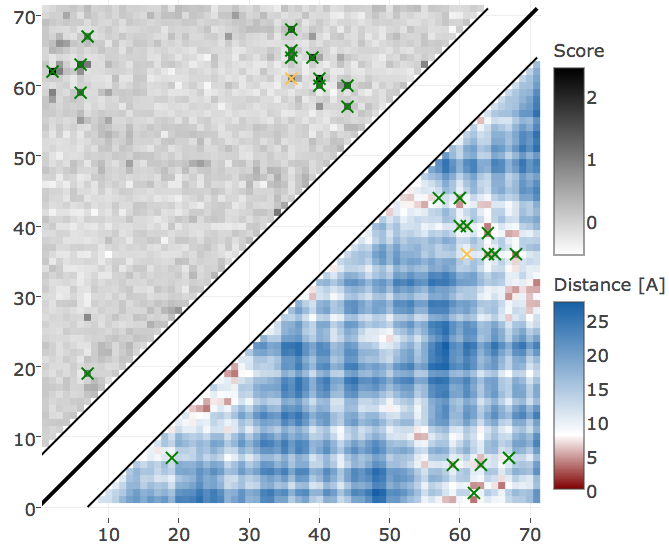
\includegraphics[width=0.49\linewidth]{img/full_likelihood/comparing_couplings/1c75A00/contact_map_pseudo-likelihood_apc_1c75A00} \includegraphics[width=0.49\linewidth]{img/full_likelihood/comparing_couplings/1c75A00/contact_map_contrastive_divergence_apc_1c75A00} 

}

\caption{Contact maps computed for protein
1c75A00. Upper left shows computed contact map and lower right shows the
native distance map. Contacts are defined according to a
\(8 \angstrom \Cb\) distance cutoff. Contact scores have been computed
as \protect\hyperlink{abbrev}{APC} corrected Frobenius norm of the
couplings. \textbf{Left} Couplings computed from pseudo-likelihood.
\textbf{Right} Couplings computed from \protect\hyperlink{abbrev}{CD}.}\label{fig:contact-maps-1c75a00}
\end{figure}

The contact maps suggest that both scores are very similar. Indeed, the
correlation between both scores is very high (Pearson's correlation
coefficient = 0.98) as can bee seen in the right plot in Figure
\ref{fig:scatter-plots-1c75a00}. Of course, by applying the average
product correction (APC), the scores are normalized with respect to the
raw contact scores (=Frobenius norm of couplings \(\wij\)). The left
plot in Figure \ref{fig:scatter-plots-1c75a00} shows the contact scores
before applying the average product correction. The raw contact scores
computed from contrastive divergence couplings are systematically
stronger than for pseudo-likelihood. Most likely this effect arises from
the weaker regularization that is used with contrastive divergence
(\(\lambda_w = 0.1L\)) than compared to pseudo-likelihood optimization
(\(\lambda_w = 0.2L\)) (see section
\ref{regularization-for-cd-with-sgd}).







\begin{figure}

{\centering \includegraphics[width=0.48\linewidth]{img/full_likelihood/comparing_couplings/1c75A00/scatter_for_pseudo-likelihoodvs_contrastive_divergence_1c75A00} \includegraphics[width=0.48\linewidth]{img/full_likelihood/comparing_couplings/1c75A00/scatter_for_pseudo-likelihoodvs_contrastive_divergence_apc_1c75A00} 

}

\caption{Contact scores computed from
pseudo-likelihood and \protect\hyperlink{abbrev}{CD} couplings for
protein 1c75A00. \textbf{Left} Frobenius norm of couplings.
\textbf{Right} Frobenius norm + \protect\hyperlink{abbrev}{APC} of
couplings.}\label{fig:scatter-plots-1c75a00}
\end{figure}

However, the contact scores have no meaning by themselfs but merely
reflect the confidence of the prediction.\\
It is more meaningful to compare the ranking of the residue pairs
imposed by the scores. The left plot in Figure
\ref{fig:ranking-pll-cd-1c75a00} compares the ordered scores of both
methods that lie very close to the diagonal which indicates that both
distribution are very similar (Kolmogorov-Smirnov pvalue = 0.0078,
Spearman rho = 0.947536). A detailed view of the top ranked predictions
is given in the right plot in Figure \ref{fig:ranking-pll-cd-1c75a00}.
The three most confident predictions are identical for both methods.
Yet, the ranks of subsequent predictions are swapped by only a few
positions which was already evident from the contact maps.












\begin{figure}

{\centering \includegraphics[width=0.48\linewidth]{img/full_likelihood/comparing_couplings/1c75A00/qq_plot_for_pseudo-likelihoodvs_contrastive_divergence_apc_1c75A00} \includegraphics[width=0.48\linewidth]{img/full_likelihood/comparing_couplings/1c75A00/comparative_value_top_ranked_contacts_for_1c75A00_method1_pseudo-likelihood_method2_contrastive_divergence_seqsep8} 

}

\caption{Comparing the ranking of highest
scoring contacts predicted with pseudo-likelihood and contrastive
divergence for protein 1c75A00. Contact scores are computed as
\protect\hyperlink{abbrev}{APC} corrected Frobenius norm of the
couplings. \textbf{Left} Q-Q plot. \textbf{Right} Contact scores for the
top 71 (=L) predictions from either method. Identical residue pairs are
connected with a line. Green indicates identical ranking of the residue
pair for both methods. Blue indicates higher ranking of the residue pair
for contrastive divergence. Red indicates higher ranking of the residue
pair for pseudo-likelihood.}\label{fig:ranking-pll-cd-1c75a00}
\end{figure}

\subsection{Protein 1ss3A00 and
1c55A00}\label{protein-1ss3a00-and-1c55a00}

When analysing sample size it was shown that by randomly selecting
0.3\protect\hyperlink{abbrev}{Neff} sequences for Gibbs sampling
improves performance especially for proteins with small
\protect\hyperlink{abbrev}{Neff} (see Figure
\ref{fig:cd-precision-sampling-size-neff}) on a small dataset used for
benchmarking (75 proteins per Neff quantile bin). This trend is still
visible on the larger test dataset but to a lesser extent (see Figure
\ref{fig:precision-cd-final-neff}).

By looking at some of these proteins with small
\protect\hyperlink{abbrev}{Neff} for which the contact score computed
from \protect\hyperlink{abbrev}{CD} couplings performs better than the
score computed from pseudo-likelihood couplings, it is striking that
\protect\hyperlink{abbrev}{CD} mainly predicts strongly conserved
positions that have high entropy.

For example, for protein 1ss3A00 (protein length=50,
\protect\hyperlink{abbrev}{Neff}=36), \protect\hyperlink{abbrev}{CD}
makes strong predictions for all pairing of the residues (8, 12, 16, 26,
30, 34) (see Figure \ref{fig:cd-predictions-small-neff-proteins}). Five
of the predicted contacts are actually true contacts. Taking a loot at
the structure it is revealed that these positions are disulfid bonds
which are strongly conserved. Another example protein 1c55A00 (protein
length = 40, Neff = 88) for which \protect\hyperlink{abbrev}{CD} makes
strong predictions for pairings beetween residues (10, 16, 20, 31, 36,
38). Again, it turns out that the five true positive predictions are
disulfid bonds (see right plot in Figure
\ref{fig:cd-predictions-small-neff-proteins}).

Interestingly, pseudo-likelihood does not predict the strongly conserved
residues pairs and therefore misses some true contacts (see Appendix
Figure \ref{fig:pll-predictions-small-neff-proteins}). However, the
predictions made by \protect\hyperlink{abbrev}{CD} are rather atypical
in a sense that coevolution methods cannot detect signals from fully
conserved columns without variation. It was unclear from the analysis of
the gradients for different samples sizes in section
\ref{cd-sampling-size} why sampling less sequences and consequently a
worse gradient estimate results in improved performance for proteins
with small \protect\hyperlink{abbrev}{Neff}. The results shown here
might be represent an explanation, such that an unperfectly trained
model tends to learn high couplings for strongly conserved residues,
which simply gives higher precision when there are many disulfide bonds.















\begin{figure}

{\centering \includegraphics[width=0.49\linewidth]{img/full_likelihood/comparing_couplings/1ss3A00/contact_map_contrastive_divergence_apc_1ss3A00} \includegraphics[width=0.49\linewidth]{img/full_likelihood/comparing_couplings/1ss3A00/1ss3A00_structure} \includegraphics[width=0.49\linewidth]{img/full_likelihood/comparing_couplings/1c55A00/contact_map_contrastive_divergence_apc_1c55A00} \includegraphics[width=0.49\linewidth]{img/full_likelihood/comparing_couplings/1c55A00/1c55A00_structure} 

}

\caption{Contact maps and
structures for protein 1ss3A00 and 1c55A00. Contact scores have been
computed as \protect\hyperlink{abbrev}{APC} corrected Frobenius norm of
the \protect\hyperlink{abbrev}{CD} couplings. Contacts are defined
according to a \(8 \angstrom \Cb\) distance cutoff. \textbf{Upper left}:
predicted contact map and native distance map for protein 1ss3A00
(protein length=50, N=42, \protect\hyperlink{abbrev}{Neff}=36).
\textbf{Upper Right}: native protein structure of 1ss3A00 with disulfide
bonds between residues pairs (8, 34), (12, 30), (16, 26). \textbf{Lower
Left} predicted contact map and native distance map for protein 1c55A00
(protein length = 40, N=115, Neff = 88) \textbf{Lower Right} native
protein structure of 1c55A00 with disulfide bonds between residues pairs
(10, 31), (16, 36), (20, 38).}\label{fig:cd-predictions-small-neff-proteins}
\end{figure}

\chapter{Random Forest Contact Prior}\label{contact-prior}

The wealth of successful meta-predictors presented in section
\ref{meta-predictors} highlights the importance to exploit other sources
of information apart from coevolution statistics. Much information about
residue interactions is typically contained in single position features
that can be predicted from local sequence profiles, such as secondary
structure, solvent accessibility or contact number, and in pairwise
features such as the contact prediction scores for residue pairs
\((i,j)\) from a simple local statistical methods as presented in
section \ref{local-methods}.

For example, predictions of secondary structure elements and solvent
accessibility are used by almost all modern machine learning predictors,
such as MetaPsicov {[}\protect\hyperlink{ref-Jones2015a}{84}{]}, NeBCon
{[}\protect\hyperlink{ref-He2017}{87}{]}, EPSILON-CP
{[}\protect\hyperlink{ref-Stahl2017}{86}{]}, PconsC3
{[}\protect\hyperlink{ref-Skwark2016}{82}{]}. Other frequently used
sequence derived features include pairwise contact potentials, sequence
separation and conservation measures such as column entropy
{[}\protect\hyperlink{ref-Jones2015a}{84},\protect\hyperlink{ref-He2017}{87},\protect\hyperlink{ref-Ma2015a}{210}{]}.

In the following sections I present a random forest classifier that uses
sequence derived features to distinguish contacts from non-contacts.
Methods section \ref{seq-features} lists all features used to train the
classifier including the aforementioned standard features as well as
some novel features.

The probabilistic predictions of the random forest model can be
introduced directly as prior information into the Bayesian statistical
model presented in the last section \ref{bayesian-approach} to improve
the overall prediction accuracy in terms of posterior probabilities.
Furthermore, contact scores from coevolution methods can be added as
additional feature to the random forest model in order to elucidate how
much the combined information improves prediction accuracy over the
single methods.

\section{Random Forest Classifiers}\label{random-forest-classifiers}

Random Forests are supervised machine learning methods that belong to
the class of ensemble methods
{[}\protect\hyperlink{ref-Ho1998}{211}--\protect\hyperlink{ref-Breiman2001}{213}{]}.
They are easy to implement, fast to train and can handle large numbers
of features due to implicit feature selection
{[}\protect\hyperlink{ref-Menze2009}{214}{]}.

Ensemble methods combine the predictions of several independent base
estimators with the goal to improve generalizability over a single
estimator. Random forests are ensembles of decision trees where
randomness is introduced in two ways:

\begin{enumerate}
\def\labelenumi{\arabic{enumi}.}
\tightlist
\item
  every tree is build on a random sample that is drawn with replacement
  from the training set and has the same size as the training set (i.e.,
  a bootstrap sample)
\item
  every split of a node is evaluated on a random subset of features
\end{enumerate}

A single decision tree, especially when it is grown very deep is highly
susceptible to noise in the training set and therefore prone to
overfitting which results in poor generalization ability. As a
consequence of randomness and averaging over many decision trees, the
variance of a random forest predictor decreases and therefore the risk
of overfitting {[}\protect\hyperlink{ref-Louppe2014}{215}{]}. It is
still advisable to restrict the depth of single trees in a random
forest, not only to counteract overfitting but also to reduce model
complexity and to speedup the algorithm.

Random forests are capable of regression and classification tasks. For
classification, predictions for new data are obtained by running each
data sample down every tree in the forest and then either apply majority
voting over single class votes or averaging the probabilistic class
predictions. Probabilistic class predictions of single trees are
computed as the fraction of training set samples of the same class in a
leaf whereas the single class vote refers to the majority class in a
leaf. Figure \ref{fig:rf-intro} visualizes the procedure of classifying
a new data sample.









\begin{figure}

{\centering \includegraphics[width=0.8\linewidth]{img/random_forest_contact_prior/intro_random_forest} 

}

\caption{Classifying new data with random forests. A new
data sample is run down every tree in the forest until it ends up in a
leaf node. Every leaf node has associated class probabilities \(p(c)\)
reflecting the fraction of training samples at this leaf node belonging
to every class \(c\). The color of the leaf nodes reflects the class
with highest probability. The predictions from all trees in form of the
class probabilties are averaged and yield the final prediction.}\label{fig:rf-intro}
\end{figure}

Typically, \emph{Gini impurity}, which is a computationally efficient
approximation to the entropy, is used as a split criterion to evaluate
the quality of a split. It measures the degree of purity in a data set
regarding class labels as \(GI = (1 - \sum_{k=1}^K p_k^2)\), where
\(p_k\) is the proportion of class \(k\) in the data set. For every
feature \(f\) in the random subset that is considered for splitting a
particular node \(N\), the \emph{decrease in Gini impurity}
\(\Delta GI_f\) will be computed as,

\[
\Delta GI_f(N_{\textrm{parent}}) = GI_f(N_{\textrm{parent}}) - p_{\textrm{left}} GI_f(N_{\textrm{left}}) - p_{\textrm{right}} GI_f(N_{\textrm{left}})
\]

where \(p_{\textrm{left}}\) and \(p_{\textrm{right}}\) refers to the
fraction of samples ending up in the left and right child node
respectively {[}\protect\hyperlink{ref-Menze2009}{214}{]}. The feature
\(f\) with highest \(\Delta GI_f\) over the two resulting child node
subsets will be used to split the data set at the given node \(N\).

Summing the \emph{decrease in Gini impurity} for a feature \(f\) over
all trees whenever \(f\) was used for a split yields the \emph{Gini
importance} measure, which can be used as an estimate of general feature
relevance. Random forests therefore are popular methods for feature
selection and it is common practice to remove the least important
features from a data set to reduce the complexity of the model. However,
feature importance measured with respect to \emph{Gini importance} needs
to be interpreted with care. The random forest model cannot distinguish
between correlated features and it will choose any of the correlated
features for a split, thereby reducing the importance of the other
features and introducing bias. Furthermore, it has been found that
feature selection based on \emph{Gini importance} is biased towards
selecting features with more categories as they will be chosen more
often for splits and therefore tend to obtain higher scores
{[}\protect\hyperlink{ref-Strobl2007}{216}{]}.

\section{Hyperparameter Optimization for Random
Forest}\label{hyperparameter-optimization-for-random-forest}

There are several hyperparameters in a random forest model that need to
be tuned to achieve best balance between predictive power and runtime.
While more trees in the random forest generally improve performance of
the model, they will slow down training and prediction. A crucial
hyperparamter is the number of features that is randomly selected for a
split at each node in a tree
{[}\protect\hyperlink{ref-Bernard2009}{217}{]}. Stochasticity introduced
by the random selection of features is a key characteristic of random
forests as it reduces correlation between the trees and thus the
variance of the predictor. Selecting many features typically increases
performance as more options can be considered for each split, but at the
same time increases risk of overfitting and decreases speed of the
algorithm. In general, random forests are robust to overfitting, as long
as there are enough trees in the ensemble and the selection of features
for splitting a node introduces sufficient stochasticity. Overfitting
can furthermore be prevented by restricting the depth of the trees,
which is known as pruning or by enforcing a minimal leaf node size
regarding the minimal number of data samples ending in a leaf node.
Again, a positive side-effect of pruning and requiring minimal leaf node
size is a speedup of the algorithm.
{[}\protect\hyperlink{ref-Louppe2014}{215}{]}

In the following, I use 5-fold cross-validation to identify the optimal
architecture of the random forest. Details about the training set and he
cross-validation procedure can be found in method section
\ref{rf-training}. First I assessed performance of models for
combinations of the parameter \emph{n\_estimators}, defining the number
of trees in the forest and the parameter \emph{max\_depth} defining the
maximum depth of the trees:

\begin{itemize}
\tightlist
\item
  \emph{n\_estimators} \(\in \{100,500,1000\}\)
\item
  \emph{max\_depth} \(\in \{10, 100, 1000, None\}\)
\end{itemize}

Figure \ref{fig:rf-gridsearch-nestimators-maxfeatures} shows that the
top five parameter combinations perform nearly identical. Random forests
with 1000 trees perform slightly better than models constituting 500
trees, irrespective of the depth of the trees. In order to keep model
complexity small, I chose \texttt{n\_estimators=1000} and
\texttt{max\_depth=100} for further analysis.














\begin{figure}

{\centering \includegraphics[width=0.9\linewidth]{img/random_forest_contact_prior/new_gridsearch/precision_vs_rank_cv_on_test_random_forest_nestimators_maxdepth_top5_notitle} 

}

\caption{Mean precision over
200 proteins against highest scoring contact predictions from random
forest models for different settings of \emph{n\_estimators} and
\emph{max\_depth}. Dashed lines show the performance of models that have
been learned on the five different subsets of training data. Solid lines
give the mean precision over the five models. Only those models are
shown that yielded the five highest mean precision values (given in
parantheses in the legend). Random forest models with 1000 trees and
maximum depth of trees of either 100, 1000 or unrestricted tree depth
perform nearly identical (lines overlap). Random forest models with 500
trees and \emph{max\_depth}=10 or \emph{max\_depth}=100 perform slightly
worse.}\label{fig:rf-gridsearch-nestimators-maxfeatures}
\end{figure}

Next, I optimized the parameters \emph{min\_samples\_leaf}, defining the
minimum number of samples required at a leaf node and
\emph{max\_features}, defining the number of randomly selected features
considered for each split using the following settings:

\begin{itemize}
\tightlist
\item
  \emph{min\_samples\_leaf} \(\in \{1, 10, 100\}\)
\item
  \emph{max\_features} \(\in \{8, 16, 38, 75 \}\) representing
  \(\sqrt{N}\), \(\log2{N}\), \(0.15N\) and \(0.3N\) respectively with
  \(N=250\) being the number of features listed in method section
  \ref{seq-features}.
\end{itemize}

Randomly selecting 30\% of features (=75 features) and requiring at
least 10 samples per leaf gives highest mean precision as can be seen in
Figure \ref{fig:rf-gridsearch-maxdepth-minsampleleaf}. I chose
\texttt{max\_features=0.30} and \texttt{min\_samples\_leaf=10} for
further analysis. Tuning the hyperparameters in a different order or on
a larger dataset gives similar results.










\begin{figure}

{\centering \includegraphics[width=0.9\linewidth]{img/random_forest_contact_prior/new_gridsearch/precision_vs_rank_cv_on_test_random_forest_maxfeatures_minsampleleaf_top5_notitle} 

}

\caption{Mean precision over 200
proteins against highest scoring contact predictions from random forest
models with different settings of \emph{min\_samples\_leaf} and
\emph{max\_features}. Dashed lines show the performance of models that
have been learned on the five different subsets of training data. Solid
lines give the mean precision over the five models. Only those models
are shown that yielded the five best mean precision values (given in
parantheses in the legend).}\label{fig:rf-gridsearch-maxdepth-minsampleleaf}
\end{figure}

In a next step I assessed dataset specific settings, such as the window
size over which single positions features will be computed, the distance
threshold to define non-contacts and the optimal proportions of contacts
and non-contacts in the training set. I used the previously identified
settings of random forest hyperparameters
(\texttt{n\_estimators=1000,\ min\_samples\_leaf=10,\ max\_depth=100,\ max\_features=0.30}).

\begin{itemize}
\tightlist
\item
  proportion of contacts/non-contacts
  \(\in \{1\!:\!2, 1\!:\!5, 1\!:\!10, 1\!:\!20 \}\) while keeping total
  dataset size fixed at 300,000 residue pairs
\item
  window size: \(\in \{5, 7, 9, 11\}\)
\item
  non-contact threshold \(\in \{8, 15, 20\}\)
\end{itemize}

As can be seen in appendix \ref{rf-window-size} and
\ref{rf-noncontact-threshold}, the default choice of using a window size
of five positions and the non-contact threshold of \(8 \angstrom\)
proves to be the optimal setting. Furthermore, using five-times as many
non-contacts as contacts in the training set results in highest mean
precision as can be seen in appendix \ref{rf-ratio-noncontacts}. These
estimates might be biased in a way since the random forest
hyperparameters have been optimized on a dataset using exactly these
optimal settings.

\section{Evaluating Random Forest Model as Contact
Predictor}\label{evaluating-random-forest-model-as-contact-predictor}

I trained a random forest classifier on the feature set described in
methods section \ref{seq-features} and using the optimal hyperparameters
identified with 5-fold cross-validation as described in the last
section.

Figure \ref{fig:rf-feature-importance} shows the ranking of the ten most
important features according to \emph{Gini importance}. Both local
statistical contact scores, \emph{OMES}
{[}\protect\hyperlink{ref-Fodor2004a}{218}{]} and
\protect\hyperlink{abbrev}{MI} (mutual information between amino acid
counts), constitute the most important features besides the mean pair
potentials acording to Miyazawa \& Jernigan
{[}\protect\hyperlink{ref-Miyazawa1999a}{219}{]} and
Li\&Fang{[}\protect\hyperlink{ref-Li2011}{69}{]}. Further important
features include the relative solvent accessibility at both pair
positions, the total percentage of gaps at both positions, the
correlation between mean isoelectric point property at both positions,
sequence separation and the beta-sheet propensity in a window of size
five around position i.
























\begin{figure}
\includegraphics[width=1\linewidth]{img/random_forest_contact_prior/feature_random_forest_optimalhyperparameters_topfeatures} \caption{Top ten features ranked according to
\emph{Gini importance}. \textbf{OMES+APC}:
\protect\hyperlink{abbrev}{APC} corrected OMES score according to
Fodor\&Aldrich {[}\protect\hyperlink{ref-Fodor2004a}{218}{]}.
\textbf{mean pair potential (Miyasawa \& Jernigan)}: average
quasi-chemical energy of transfer of amino acids from water to the
protein environment {[}\protect\hyperlink{ref-Miyazawa1999a}{219}{]}.
\textbf{MI+APC}: \protect\hyperlink{abbrev}{APC} corrected mutual
information between amino acid counts (using pseudo-counts).
\textbf{mean pair potential (Li\&Fang)}: average general contact
potential by Li \& Fang {[}\protect\hyperlink{ref-Li2011}{69}{]}.
\textbf{rel. solvent accessibilty i(j)}: RSA score computed with
Netsurfp (v1.0) {[}\protect\hyperlink{ref-Petersen2009a}{220}{]} for
position i(j). \textbf{pairwise gap\%}: percentage of gapped sequences
at either position i and j. \textbf{correlation mean isoelectric
feature}: Pearson correlation between the mean isoelectric point feature
(according to Zimmermann et al., 1968) for positions i and j.
\textbf{sequence separation}: \textbar{}j-i\textbar{}. \textbf{beta
sheet propensity window(i)}: beta-sheet propensity according to Psipred
{[}\protect\hyperlink{ref-Jones1999}{221}{]} computed within a window of
five positions around i. eatures are described in detail in methods
section \ref{seq-features}.}\label{fig:rf-feature-importance}
\end{figure}

Many features have low \emph{Gini importance} scores which means they
are rarely considered for splitting a node and can most likely be
removed from the dataset. Removing irrelevant features from the dataset
is a convenient procedure to reduce model complexity. It has been found,
that prediction performance might even increase after removing the most
irrelevant features {[}\protect\hyperlink{ref-Menze2009}{214}{]}. For
example, during the development of \emph{EPSILON-CP}, a deep neural
network method for contact prediction, the authors performed feature
selection using boosted trees. By removing 75\% of the most
non-informative features (mostly features related to amino acid
composition), the performance of their predictor increased slightly
{[}\protect\hyperlink{ref-Stahl2017}{86}{]}. Other studies have also
emphasized the importance of feature selection to improve performance
and reduce model complexity
{[}\protect\hyperlink{ref-Cheng2007}{67},\protect\hyperlink{ref-Li2011}{69}{]}.







\begin{figure}
\includegraphics[width=0.9\linewidth]{img/random_forest_contact_prior/precision_vs_rank_featureselection_random_forest_optimized_hyperparameters} \caption{Mean precision of top
ranked predictions over 200 proteins for random forest models trained on
subsets of features of decreasing importance. Subsets of features have
been selected as described in methods section
\ref{rf-feature-selection}.}\label{fig:rf-feature-selection-performance}
\end{figure}












\begin{figure}
\includegraphics[width=0.9\linewidth]{img/random_forest_contact_prior/precision_vs_rank_notitle} \caption{Mean precision for top ranked contacts on a
test set of 1000 proteins. \textbf{pseudo-likelihood} =
\protect\hyperlink{abbrev}{APC} corrected Frobenius norm of couplings
computed with pseudo-likelihood. \textbf{random forest} = random forest
model trained on 75 sequence derived features. \textbf{OMES} =
\protect\hyperlink{abbrev}{APC} corrected \emph{OMES} contact score
according to Fodor\&Aldrich
{[}\protect\hyperlink{ref-Fodor2004a}{218}{]}. \textbf{mutual
information} = \protect\hyperlink{abbrev}{APC} corrected mutual
information between amino acid counts (using pseudo-counts).}\label{fig:performance-rf}
\end{figure}

As described in methods section \ref{rf-feature-selection}, I performed
feature selection by evaluating model performance on subsets of features
of decreasing importance. Most models trained on subsets of the total
feature space perform nearly identical compared to the model trained on
all features, as can be seen in Figure
\ref{fig:rf-feature-selection-performance}. Performance of the random
forest models drops noticeably when using only the 25 most important
features. For the further analysis I am using the random forest model
trained on the 75 most important features as this model constitutes the
smallest set of features while performing nearly identical compared to
the model trained on the complete feature set.

Figure \ref{fig:performance-rf} shows the mean precision for the random
forest model trained on the 75 most important features. The random
forest model has a mean precision of 0.33 for the top \(0.5\cdot L\)
contacts compared to a precision of 0.47 for pseudo-likelihood.
Furthermore, the random forest model improves approximately ten
percentage points in precision over the local statistical contact
scores, \emph{OMES} and mutual information (MI). Both methods comprise
important features of the random forest model as can be seen in Figure
\ref{fig:rf-feature-importance}.

When analysing performance with respect to alignment size it can be
found that the random forest model outperforms the pseudo-likelihood
score for small alignments (see Figure \ref{fig:performance-neff-rf}).\\
Both, local statistial models \emph{OMES} and
\protect\hyperlink{abbrev}{MI} also perform weak on small alignments,
leading to the conclusion that the remaining sequence derived features
are highly relevant when the alignment contains only few sequences. This
finding is expected, as it is well known that models trained on simple
sequence features perform almost independent of alignment size
{[}\protect\hyperlink{ref-Skwark2016}{82},\protect\hyperlink{ref-Stahl2017}{86}{]}.

\section{Using Contact Scores as Additional
Features}\label{using-contact-scores-as-additional-features}















\begin{figure}
\includegraphics[width=0.9\linewidth]{img/random_forest_contact_prior/additional_contat_score_features/precision_vs_rank_rf_pll_cd} \caption{Mean precision for top
ranked contacts on a test set of 1000 proteins. \textbf{random forest
(pLL, CD)} random forest model trained on sequence features and the
pseudo-likelihood and contrastive divergence contact scores.
\textbf{random forest (pLL)} random forest model trained on sequence
features and the pseudo-likelihood contact score. \textbf{random forest
(CD)} random forest model trained on sequence features and the
contrastive divergence contact score. \textbf{contrastive divergence}
\protect\hyperlink{abbrev}{APC} corrected Frobenius norm of couplings
computed with contrastive divergence. \textbf{pseudo-likelihood} =
\protect\hyperlink{abbrev}{APC} corrected Frobenius norm of couplings
computed with pseudo-likelihood. \textbf{random forest} = random forest
model trained on 75 sequence derived features.}\label{fig:performance-rf-additional-features}
\end{figure}

Figure \ref{fig:performance-neff-rf} shows that the random forest
predictor improves over the pseudo-likelihood coevolution method when
the alignment consists of only few sequences. In order to assess this
improvement in a more direct manner, it is possible to build a combined
random forest predictor that is not only trained on the sequence derived
features but also on the pseudo-likelihood contact score as an
additional feature. As expected, the pseudo-likelihood score comprises
the most important feature in the model (see Appendix Figure
\ref{fig:feature-importance-rf-with-pll-score}) followed by the same
sequence features that were found in the previous analysis in Figure
\ref{fig:rf-feature-importance}. The model trained on the 76 most
relevant features performs as well as the model trained on the full
feature set and was used in the benchmark shown in Figure
\ref{fig:performance-rf-additional-features}. The combination of simple
sequence features with the coevolution pseudo-likelihood contact score
indeed improves predictive power for the random forest model over both
single approaches. Especially for small alignments, the improvement is
substantial (about 12\%) as can be seen in in the left plot in Figure
\ref{fig:performance-neff-rf-additional-features}. In contrast, the
improvement on large alignments (right plot in Figure
\ref{fig:performance-neff-rf-additional-features}) is smaller (about
5\%), as the gain from simple sequence features compared to the much
more powerful coevolution signals is neglectable.

Similarly, the contact scores derived from couplings computed with
\protect\hyperlink{abbrev}{CD} in chapter
\ref{optimizing-full-likelihood} can be added as a feature instead of
the pseudo-likelihood score or besides the pseudo-likelihood contact
score. The three resultant models perform comparably (see Figure
\ref{fig:performance-rf-additional-features}) and apparantly, there is
minor information gain by adding both coevolution contact scores. Since
it has been shown in section \ref{comparing-pll-cd} that
pseudo-likelihood and contrastive divergence contact scores are highly
correlated, resulting in very similar rankings for residue pairs, it is
not surprising that the random forest model including both coevolution
scores does not improve over the random forest model including only one
of both scores.











\begin{figure}
\includegraphics[width=1\linewidth]{img/random_forest_contact_prior/additional_contat_score_features/precision_vs_rank_facetted_by_neff_rf_pll_cd} \caption{Mean precision for
top ranked contacts on a test set of 1000 proteins splitted into four
equally sized subsets with respect to \protect\hyperlink{abbrev}{Neff}.
Subsets are defined according to quantiles of
\protect\hyperlink{abbrev}{Neff} values. \textbf{Left}: Subset of
proteins with \protect\hyperlink{abbrev}{Neff} \textless{} Q1.
\textbf{Right}: Subset of proteins with Q3 \textless{}=
\protect\hyperlink{abbrev}{Neff} \textless{} Q4. Methods are the same as
in Figure \ref{fig:performance-rf-additional-features}}\label{fig:performance-neff-rf-additional-features}
\end{figure}

\chapter{A Bayesian Statistical Model for Residue-Residue Contact
Prediction}\label{a-bayesian-statistical-model-for-residue-residue-contact-prediction}

All methods so far predict contacts by finding the one solution of
parameters \(\via\) and \(\wijab\) that maximizes a regularized version
of the log likelihood of the \protect\hyperlink{abbrev}{MSA} and in a
second step transforming the \protect\hyperlink{abbrev}{MAP} estimates
of the couplings \(\w^*\) into heuristic contact scores (see
Introduction \ref{pseudo-likelihood}). Apart from the heuristic
transformation that omits meaningful information comprised in the
coupling matrices \(\wij\) as discussed in section
\ref{interpreting-coupling-matrices}, using the
\protect\hyperlink{abbrev}{MAP} estimate of the parameters instead of
the true distribution has the decisive disadvantage of concealing the
uncertainty of the estimates.

The next sections present the derivation of a principled Bayesian
statistical approach for contact prediction eradicating these
deficiencies. The model provides estimates of the posterior probability
distributions of contact states \(\cij\) for all residues pairs \(i\)
and \(j\), given the \protect\hyperlink{abbrev}{MSA} \(\X\). A true
contact (contact state \(\cij\eq1\)) is defined as two residues whose
\(\Cb\)-\(\Cb\) distance \(\le 8 \angstrom\), whereas a residue pair
with \(\Cb\)-\(\Cb\) distance \(>8 \angstrom\) is considered not to be
in physical contact (contact state \(\cij\eq0\)). The parameters
\((\v, \w)\) of the \protect\hyperlink{abbrev}{MRF} model describing the
probability distribution of the sequences in the
\protect\hyperlink{abbrev}{MSA} are treated as hidden parameters that
can be integrated out using an approximation to the posterior
distribution of couplings \(\w\). This approach also allows to
explictely model the dependence of coupling coeffcients \(\wij\) on
contacts/non-contacts as a mixture of Gaussians with contact state
dependent mixture weights and thus can even learn correlations between
couplings.

\section{Computing the Posterior Probabiilty of a
Contact}\label{overview-posterior-distances}

The joint probability of contact states \(\c\) and
\protect\hyperlink{abbrev}{MRF} model parameters \((\v, \w)\) given the
\protect\hyperlink{abbrev}{MSA} \(\X\) and a set of sequence derived
features \(\phi\) (such as listed in method section \ref{seq-features}),
can be written as a hierarchical Bayesian model of the form:

\begin{align}
        p(\c, \v, \w | \X, \phi) &\propto p(\X | \v, \w) p(\v, \w | \c) \, p(\c | \phi ) \, .
\label{eq:hierarchical-bayesian-model}
\end{align}

The ultimate goal is to compute the posterior probability of the contact
states, \(p(\c | \X, \phi)\), that can be obtained by treating the
parameters \((\v, \w)\) as hidden variables and marginalizing over these
parameters,

\begin{align}
    p(\c | \X , \phi) &\propto  p(\X | \c) p(\c | \phi)\\
    p(\X | \c) &= \int \int p(\X | \v,\w) \, p(\v, \w | \c) \,d\v\,d\w  \; .
\label{eq:integrate-out-vw}
\end{align}

The single potentials \(\v\) will be fixed at their best estimate
\(\v^*\) (see method section \ref{prior-v}) by using a very tight prior
\(p(\v) = \Gauss(\v|\v^*,\lambda_v^{-1} \I) \rightarrow \delta(\v-\v*)\)
for \(\lambda_v \rightarrow \infty\) that acts as a delta function. This
allows the replacement of the intergral over \(\v\) with the value of
the integrand at its mode \(\v^*\).

Computing the integral over \(\w\) can be achieved by factorizing the
integrand into factors over \((i,j)\) and performing each integration
over the coupling coefficients \(\wij\) for \((i,j)\) separately.

For that account, the prior over \(\w\) will be modelled as a product
over independent contributions over \(\wij\) with \(\wij\) depending
only on the contact state \(\cij\), which is described in detail in
method section \ref{coupling-prior}. The prior over the \emph{Potts}
model parameters then yields,

\begin{equation}
  p(\v,\w|\c) = \Gauss(\v|\v^*,\lambda_v^{-1} \I) \, \prod_{1\le i<j\le L} p(\wij|\cij) \; .
\label{eq:definition-parameter-prior}
\end{equation}

Furthermore, method section \ref{laplace-approx} proposes an
approximation to the regularised likelihood,
\(p(\X | \v,\w) \, p(\v, \w)\), with a Gaussian distribution that
facilitates the analytical solution of the integral in eq.
\eqref{eq:integrate-out-vw}. The detailed derivation of the solution to
the integral is covered in method section
\ref{likelihood-fct-distances}.

Finally, the marginals
\(p(\cij | \X, \phi) = \int p(\c | \X, \phi) d \c_{\backslash ij}\),
where \(\c_{\backslash ij}\) is the vector containing all coordinates of
\(\c\) except \(\cij\) can be computed to obtain the posterior
probability distribution of the contact states (see method section
\ref{posterior-of-rij}).

\section{Training the Hyperparameters in the Likelihood Function of
Contact States}\label{bayesian-model-training-hyperparameters}

The likelihood function of contact states, given in eq.
\eqref{eq:pXr-final}, is obtained by solving the integral in eq.
\eqref{eq:integrate-out-vw}. It contains the hyperparameters
\(\gamma_k(\cij)\), \(\muk\) and \(\Lk\) representing the weights, mean
vectors and precision matrices of the \(K\) Gaussian components of the
contact state dependent coupling prior, respectively. The
hyperparameters are trained by maximizing the logarithm of the
likelihood over a set of training \protect\hyperlink{abbrev}{MSAs} as
described in detail in method section \ref{training-hyperparameters}.

The \protect\hyperlink{abbrev}{MAP} estimates of the coupling parameters
\(\wij^*\) is are needed to compute the Hessian of the regularized
\emph{Potts} model likelihood, which again is needed for the Gaussian
approximation to the likelihood. For that purpose, I tested couplings
\(\wij^*\) obtained from pseudo-likelihood maximization as well as the
couplings \(\wij^*\) obtained by maximizing the full likelihood with
\protect\hyperlink{abbrev}{CD}.

\section{Training on couplings from pseudo-likelihood
maximization}\label{training-on-couplings-from-pseudo-likelihood-maximization}

I trained models with \(K \in \{3,5,10\}\) Gaussian mixture components
with diagonal precision matrices \(\Lk\) and a zero-component that is
fixed at \(\mu_0=0\). Convergence has only been observed for Gaussian
mixture with \(K \eq 3\) components and for the smallest datasets with
10000 and 100,000 residue pairs per contact class. However, the
resultant mixtures are consistent regardless of the dataset size and
independent repeated trainings.

Figure \ref{fig:stats-pll-3comp-100k} shows the statistics of the
hyperparameters for a three component Gaussian mixture trained on
100,000 residue pairs per contact class. The zeroth component, with
\(\mu_0=0\) has a weight for 0.88 for the non-contact class whereas it
has only weight 0.5 in the contact class, which is expected given that
the couplings \(\wijab\) for non-contacts have a much tighter
distribution around zero than contacts. Component 2 has the highest
standard deviations and the broadest spread. It is not surprising that
it has low (\(g_2(0) \eq 0.0026\)) component weight for non-contacts but
a higher weight (\(g_2(1) \eq 0.14\)) for contacts.







\begin{figure}
\includegraphics[width=1\linewidth]{img/bayesian_model/pll/3/stats-pll-3comp-100k} \caption{Statistics for the hyperparameters,
\(\gamma_k(\cij)\), \(\muk\) and \(\Lk\) obtained after 371 iterations.
Trained on 100,000 residue pairs per contact class for a three component
Gaussian mixture and using pseudo-likelihood couplings to estimate the
Hessian.}\label{fig:stats-pll-3comp-100k}
\end{figure}








\begin{figure}
\includegraphics[width=0.49\linewidth]{img/bayesian_model/pll/3/aa_pll-3comp-300k-nolegend} \includegraphics[width=0.49\linewidth]{img/bayesian_model/pll/3/ww_pll-3comp-300k-nolegend} \includegraphics[width=0.49\linewidth]{img/bayesian_model/pll/3/er_pll-3comp-300k-nolegend} \includegraphics[width=0.49\linewidth]{img/bayesian_model/pll/3/ee_pll-3comp-300k-nolegend} \caption{Visualisation of 1diemnsion
projection for AA. Green solid line: Gaussian mixture for contacts. Blue
solid line: Gaussian mixture for non-contacts. Light blue dashed line:
Gaussian component 0. Dark blue dashed line: Gaussian component 1. Light
Green dashed line: Gaussian component 2. Color code is identical to
Figure \ref{fig:stats-pll-3comp-100k}}\label{fig:vis1d-aa-pll-3comp-300k}
\end{figure}

\chapter{Methods}\label{methods}

\section{Dataset}\label{dataset}

A protein dataset has been constructed from the CATH (v4.1)
{[}\protect\hyperlink{ref-Sillitoe2015}{222}{]} database for
classification of protein domains. All CATH domains from classes
1(mainly \(\alpha\)), 2(mainly \(\beta\)), 3(\(\alpha+\beta\)) have been
selected and filtered for internal redundancy at the sequence level
using the \texttt{pdbfilter} script from the
HH-suite{[}\protect\hyperlink{ref-Remmert2012}{179}{]} with an E-value
cutoff=0.1. The dataset has been split into ten subsets aiming at the
best possible balance between CATH classes 1,2,3 in the subsets. All
domains from a given CATH topology (=fold) go into the same subsets, so
that any two subsets are non-redundant at the fold level. Some
overrepresented folds (e.g.~Rossman Fold) have been subsampled ensuring
that in every subset each class contains at max 50\% domains of the same
fold. Consequently, a fold is not allowed to dominate a subset or even a
class in a subset. In total there are 6741 domains in the dataset.

Multiple sequence alignments were built from the CATH domain sequences
(\href{http://www.cathdb.info/version/current/domain/3cdjA03/sequence}{COMBS})
using HHblits {[}\protect\hyperlink{ref-Remmert2012}{179}{]} with
parameters to maximize the detection of homologous sequences:

\texttt{hhblits\ -maxfilt\ 100000\ -realign\_max\ 100000\ -B\ 100000\ -Z\ 100000\ -n\ 5\ -e\ 0.1\ -all\ hhfilter\ -id\ 90\ -neff\ 15\ -qsc\ -30}

The COMBS sequences are derived from the SEQRES records of the PDB file
and sometimes contain extra residues that are not resolved in the
structure. Therefore, residues in PDB files have been renumbered to
match the COMBS sequences. The process of renumbering residues in PDB
files yielded ambigious solutions for 293 proteins, that were removed
from the dataset. Another filtering step was applied to remove 80
proteins that do not hold the following properties:

\begin{itemize}
\tightlist
\item
  more than 10 sequences in the multiple sequence alignment (\(N>10\))
\item
  protein length between 30 and 600 residues (\(30 \leq L \leq 600\))
\item
  less than 80\% gaps in the multiple sequence alignment (percent gaps
  \textless{} 0.8)
\item
  at least one residue-pair in contact at \(C_\beta < 8\angstrom\) and
  minimum sequence separation of 6 positions
\end{itemize}

The final dataset is comprised of \textbf{6368} proteins with almost
evenly distributed CATH classes over the ten subsets (Figure
\ref{fig:dataset-cath-topologies}).





\begin{figure}
\includegraphics[width=1\linewidth]{img/dataset_statistics/cath_topologies_stacked_reative_notitle} \caption{Distribution of CATH classes
(1=mainly \(\alpha\), 2=mainly \(\beta\), 3=\(\alpha-\beta\)) in the
dataset and the ten subsets. }\label{fig:dataset-cath-topologies}
\end{figure}

\section{Computing Pseudo-Likelihood
Couplings}\label{computing-pseudo-likelihood-couplings}

Dr Stefan Seemayer has reimplementated the open-source software CCMpred
{[}\protect\hyperlink{ref-Seemayer2014}{100}{]} in Python. CCMpred
optimizes the regularized negative pseudo-log-likelihood using a
conjugate gradients optimizer. Based on a fork of his private github
repository I continued development and extended the software, which is
now called CCMpredPy. It will soon be available at
\url{https://github.com/soedinglab/CCMpredPy}. All computations in this
thesis are performed with CCMpredPy unless stated otherwise.

\subsection{Differences between CCMpred and
CCMpredpy}\label{diff-ccmpred-ccmpredpy}

CCMpredPy differs from CCMpred
{[}\protect\hyperlink{ref-Seemayer2014}{100}{]} which is available at
\url{https://github.com/soedinglab/CCMpred} in several details:

Initialization of potentials \(\v\) and \(\w\): - CCMpred initializes
single potentials \(\v_i(a) = \log f_i(a) - \log f_i(a= "-")\) with
\(f_i(a)\) being the frequency of amino acid a at position i and
\(a="-"\) representing a gap. A single pseudo-count has been added
before computing the frequencies. Pair potentials \(\w\) are intialized
at 0. - CCMpredPy initializes single potentials \(\v\) with the
\protect\hyperlink{abbrev}{ML} estimate of single potentials (see
section \ref{prior-v}) using amino acid frequencies computed as
described in section \ref{amino-acid-frequencies}. Pair potentials
\(\w\) are initialized at 0.

Regularization:

\begin{itemize}
\tightlist
\item
  CCMpred uses a Gaussian regularization prior centered at zero for both
  single and pair potentials. The regularization coefficient for single
  potentials \(\lambda_v = 0.01\) and for pair potentials
  \(\lambda_w = 0.2 * (L-1)\) with \(L\) being protein length.
\item
  CCMpredPy uses a Gaussian regularization prior centered at zero for
  the pair potentials. For the single potentials the Gaussian
  regularization prior is centered at the \protect\hyperlink{abbrev}{ML}
  estimate of single potentials (see section \ref{prior-v}) using amino
  acid frequencies computed as described in section
  \ref{amino-acid-frequencies}. The regularization coefficient for
  single potentials \(\lambda_v = 10\) and for pair potentials
  \(\lambda_w = 0.2 * (L-1)\) with \(L\) being protein length.
\end{itemize}

Default settings for CCMpredPy have been chosen to best reproduce
CCMpred results. A benchmark over a subset of approximately 3000
proteins confirms that performance measured as
\protect\hyperlink{abbrev}{PPV} for both methods is almost identical
(see Figure \ref{fig:cmmpredvanilla-vs-ccmpredpy}).










\begin{figure}
\includegraphics[width=1\linewidth]{img/methods/ccmpredvanilla_vs_ccmpredpy_precision_vs_rank} \caption{Mean precision over 3124
proteins of top ranked contacts computed as
\protect\hyperlink{abbrev}{APC} corrected Frobenius norm of couplings.
Couplings have been computed with CCMpred
{[}\protect\hyperlink{ref-Seemayer2014}{100}{]} and CCMpredPy as
specified in the legend. Specific flags that have been used to run both
methods are described in detail in the text (see section
\ref{diff-ccmpred-ccmpredpy}).}\label{fig:cmmpredvanilla-vs-ccmpredpy}
\end{figure}

The benchmark in Figure \ref{fig:cmmpredvanilla-vs-ccmpredpy} as well as
all contacts predicted with CCMpred and CCMPredPy (using
pseudo-likelihood) in my thesis have been computed using the following
flags:

flags for computing pseudo-likelihood couplings with CCMpredPy:

\begin{verbatim}
--maxit 250                  # Compute a maximum of MAXIT operations
--center-v                   # Use a Gaussian prior for single potentials 
                             # centered at ML estimate v*          
--reg-l2-lambda-single 10    # regularization coefficient for 
                             # single potentials
--reg-l2-lambda-pair-factor 0.2   # regularization coefficient for 
                                  # pairwise potentials computed as 
                                  # reg-l2-lambda-pair-factor * (L-1)
--pc-uniform        # use uniform pseudocounts 
                    # (1/21 for 20 amino acids + 1 gap state) 
--pc-count 1        # defining pseudo count admixture coefficient 
                    # rho = pc-count/( pc-count+ Neff)
--epsilon 1e-5      # convergence criterion for minimum decrease 
                    # in the last K iterations
--ofn-pll           # using pseudo-likelihood as objective function
--alg-cg            # using conjugate gradient to optimize 
                    # objective function
\end{verbatim}

flags for computing pseudo-likelihood couplings with CCMpred:

\begin{verbatim}
-n 250    # NUMITER:  Compute a maximum of NUMITER operations
-l 0.2    # LFACTOR:  Set pairwise regularization coefficients 
          # to LFACTOR * (L-1) 
-w 0.8    # IDTHRES:  Set sequence reweighting identity 
          # threshold to IDTHRES
-e 1e-5   # EPSILON:  Set convergence criterion for minimum 
          # decrease in the last K iterations to EPSILON
\end{verbatim}

\section{Sequence Reweighting}\label{seq-reweighting}

As discussed in section \ref{challenges}, sequences in a
\protect\hyperlink{abbrev}{MSA} do not represent independent draws from
a probabilistic model. To reduce the effects of overrepresented
sequences, typically a simple weighting strategy is applied that assigns
a weight to each sequence that is the inverse of the number of similar
sequences according to an identity threshold
{[}\protect\hyperlink{ref-Stein2015a}{99}{]}. It has been found that
reweighting improves contact prediction performance
{[}\protect\hyperlink{ref-Jones2012}{65},\protect\hyperlink{ref-Morcos2011}{95},\protect\hyperlink{ref-Buslje2009}{176}{]}
significantly but results are robust against the choice of the identity
threshold in a range between 0.7 and 0.9
{[}\protect\hyperlink{ref-Morcos2011}{95}{]}. An identity threshold of
0.8 has been used for all analyses in this thesis.

Every sequence \(x_n\) of length \(L\) in an alignment with \(N\)
sequences has an associated weight \(w_n = 1/m_n\), where \(m_n\)
represents the number of similar sequences:

\begin{equation} 
  w_n = \frac{1}{m_n}, m_n = \sum_{m=1}^N I \left( ID(x_n, x_m) \geq 0.8 \right) \\
  ID(x_n, x_m)=\frac{1}{L} \sum_{i=1}^L I(x_n^i = x_m^i)
  \label{eq:seqweight}
\end{equation}

The number of effective sequences \(\mathbf{\neff}\) of an alignment is
then the number of sequence clusters computed as:

\begin{equation} 
  \neff = \sum_{n=1}^N w_n
  \label{eq:neff}
\end{equation}

TODO: Plot Performance for Seq weighting

\section{Computing Amino Acid Frequencies}\label{amino-acid-frequencies}

Single and pairwise amino acid frequencies are computed from amino acid
counts of weighted sequences as described in the last section
\ref{seq-reweighting} and additional pseudocounts that are added to
improve numerical stability.

Let \(a,b \in \{1,\ldots,20\}\) be amino acids and
\(q_0(x_i=a), q_0(x_i=a,x_j=b)\) be the empirical single and pair
frequencies without pseudocounts. The empirical single and pair
frequencies with pseudocounts, \(q(x_i=a), q(x_i=a, x_j=b)\), are
defined

\begin{align}
    q(x_i \eq a) :=& (1-\tau) \;  q_0(x_i \eq a) + \tau \tilde{q}(x_i\eq a) \\
    q(x_i \eq a, x_j \eq b) :=& (1-\tau)^2  \; [ q_0(x_i \eq a, x_j \eq b) - q_0(x_i \eq a)  q_0(x_j \eq b) ] + \nonumber\\
                            & q(x_i \eq a) \; q(x_j \eq b) 
\label{eq:pseudocounts}
\end{align}

with \(\tilde{q}(x_i \eq a) := f(a)\) being background amino acid
frequencies and \(\tau \in [0,1]\) is a pseudocount admixture
coefficient, which is a function of the diversity of the multiple
sequence alignment:

\begin{equation}
    \tau = \frac{N_\mathrm{pc}}{(N_\mathrm{eff} + N_\mathrm{pc})}
\label{eq:tau}
\end{equation}

where \(N_{pc} > 0\).

The formula for \(q(x_i \eq a, x_j \eq b)\) in the second line in eq
\eqref{eq:pseudocounts} was chosen such that for \(\tau \eq0\) we obtain
\(q(x_i \eq a, x_j \eq b) = q_0(x_i \eq a, x_j \eq b)\), and furthermore
\(q(x_i \eq a, x_j \eq b) = q(x_i \eq a) q(x_j \eq b)\) exactly if
\(q_0(x_i \eq a, x_j \eq b) = q_0(x_i \eq a) q_0(x_j \eq b)\).

\section{Regularization}\label{methods-regularization}

\emph{CCMpredPy} uses an L2-regularization per default that pushes the
single and pairwise terms smoothly towards zero and is equivalent to the
logarithm of a zero-centered Gaussian prior,

\begin{align}
  R(\v, \w)  &= \log \left[ \mathcal{N}(\v | \v^*, \lambda_v^{-1} I) \mathcal{N}(\w | \w^*, \lambda_w^{-1} I) \right] \nonumber \\
             &= -\frac{\lambda_v}{2} ||\v-\v^*||_2^2 - \frac{\lambda_w}{2} ||\w-w^*||_2^2 + \text{const.} \; ,
\label{eq:l2-reg}
\end{align}

where the regularization coefficients \(\lambda_v\) and \(\lambda_w\)
determine the strength of regularization.

The regularization coefficient \(\lambda_w\) for couplings \(\w\) is
defined with respect to protein length \(L\) owing to the fact that the
number of possible contacts in a protein increases quadratically with
\(L\) whereas the number of observed contacts only increases linearly as
can be seen in Figure \ref{fig:number-contacts-against-L}.





\begin{figure}

{\centering \includegraphics[width=0.9\linewidth]{img/full_likelihood/no_contacts_vs_protein_length_thr8} 

}

\caption{Number of contacts
(\(\Cb < 8 \angstrom\)) with respect to protein length and sequence
separation has a linear relationship.}\label{fig:number-contacts-against-L}
\end{figure}

Most previous pseudo-likelihood approaches using L2-regularization for
pseudo-likelihood optimization set \(\v^* \eq \w^* \eq \mathbf{0}\)
{[}\protect\hyperlink{ref-Seemayer2014}{100}--\protect\hyperlink{ref-Kamisetty2013}{102}{]}.
A different choice for \(v^*\) is discussed in section \ref{prior-v}
that is is used per default with \emph{CCMpredPy}. The single potentials
will not be optimized with \protect\hyperlink{abbrev}{CD} but will be
fixed at \(v^*\) given in eq. \eqref{eq:prior-v}. Furthermore,
\emph{CCMpredPy} uses regularization coefficients \(\lambda_v \eq 10\)
and \(\lambda_w \eq 0.2\cdot(L-1)\) for pseudo-likelihood optimization
and the choice for \(\lambda_w\) used with
\protect\hyperlink{abbrev}{CD} is discussed in section
\ref{regularization-for-cd-with-sgd}.

\section{The Potts Model}\label{potts-full-likelihood}

The \(N\) sequences of the \protect\hyperlink{abbrev}{MSA} \(\X\) of a
protein family are denoted as \({\seq_1, ..., \seq_N}\). Each sequence
\(\seq_n = (\seq_{n1}, ..., \seq_{nL})\) is a string of \(L\) letters
from an alphabet indexed by \(\{0, ..., 20\}\), where 0 stands for a gap
and \(\{1, ... , 20\}\) stand for the 20 types of amino acids. The
likelihood of the sequences in the \protect\hyperlink{abbrev}{MSA} of
the protein family is modelled with a \emph{Potts Model}, as described
in detail in section \ref{maxent}:

\begin{align}
    p(\X | \v, \w) &= \prod_{n=1}^N p(\seq_n | \v, \w) \nonumber \\
                   &= \prod_{n=1}^N \frac{1}{Z(\v, \w)} \exp \left( \sum_{i=1}^L v_i(x_{ni}) \sum_{1 \leq i < j \leq L} w_{ij}(x_{ni}, x_{nj}) \right)
\end{align}

The coefficients \(\via\) and \(\wijab\) are referred to as single
potentials and couplings, respectively that describe the tendency of an
amino acid a (and b) to (co-)occur at the respective positions in the
\protect\hyperlink{abbrev}{MSA}. \(Z(\v, \w)\) is the partition function
that normalizes the probability distribution \(p(\seq_n |\v, \w)\):

\begin{equation}
  Z(\v, \w) = \sum_{y_1, ..., y_L = 1}^{20} \exp \left( \sum_{i=1}^L v_i(y_i) \sum_{1 \leq i < j \leq L} w_{ij}(y_i, y_j)  \right)
\end{equation}

The log likelihood is

\begin{align}
    \LL &= \log p(\X | \v, \w) \nonumber \\
        &= \sum_{n=1}^N \left [  \sum_{i=1}^L v_i(x_{ni}) \sum_{1 \leq i < j \leq L} w_{ij}(x_{ni}, x_{nj})   \right ] - N \log Z(\v, \w) .
\end{align}

The gradient of the log likelihood has single components

\begin{align}
    \frac{\partial \LL}{\partial \via} &= \sum_{n=1}^N I(x_{ni} \eq a)  - N \frac{\partial}{\partial \via} \log Z(\v,\w) \nonumber\\
                                        &= \sum_{n=1}^N I(x_{ni} \eq a) - N \sum_{y_1,\ldots,y_L=1}^{20} \!\! \frac{ \exp \left( \sum_{i=1}^L v_i(y_i) + \sum_{1 \le i < j \le L} w_{ij}(y_i,y_j) \right)}{Z(\v,\w)}  I(y_i \eq a) \nonumber\\
                                        &=  N q(x_{i} \eq a) - N p(x_i \eq a | \v,\w) 
\label{eq:gradient-LL-single}
\end{align}

and pair components

\begin{align}
    \frac{\partial \LL}{\partial \wijab} =& \sum_{n=1}^N I(x_{ni}=a, x_{nj}=b)  - N \frac{\partial}{\partial \wijab} \log Z(\v,\w) \nonumber\\
                                        =& \sum_{n=1}^N I(x_{ni} \eq a, x_{nj} \eq b) \nonumber\\
                                        & - N \sum_{y_1,\ldots,y_L=1}^{20} \!\! \frac{ \exp \left( \sum_{i=1}^L v_i(y_i) + \sum_{1 \le i < j \le L} w_{ij}(y_i,y_j) \right)}{Z(\v,\w)}  I(y_i \eq a, y_j \eq b) \nonumber\\
                                        =&  N q(x_{i} \eq a, x_{j} \eq b) - N \sum_{y_1,\ldots,y_L=1}^{20} p(y_1, \ldots, y_L | \v,\w) \, I(y_i \eq a, y_j \eq b) \nonumber\\
                                        =&  N q(x_{i} \eq a, x_{j} \eq b) - N p(x_i \eq a, x_j \eq b | \v,\w) 
\label{eq:gradient-LL-pair}
\end{align}

\subsection{Treating Gaps as Missing Information}\label{gap-treatment}

Treating gaps explicitly as 0'th letter of the alphabet will lead to
couplings between columns that are not in physical contact. To see why,
imagine a hypothetical alignment consisting of two sets of sequences as
it is illustrated in Figure \ref{fig:gap-treatment}. The first set has
sequences covering only the left half of columns in the MSA, while the
second set has sequences covering only the right half of columns. The
two blocks could correspond to protein domains that were aligned to a
single query sequence. Now consider couplings between a pair of columns
\(i, j\) with \(i\) from the left half and \(j\) from the right half.
Since no sequence (except the single query sequence) overlaps both
domains, the empirical amino acid pair frequencies
\(q(x_i = a, x_j = b)\) will vanish for all \(a, b \in \{1,... , L\}\).










\begin{figure}

{\centering \includegraphics[width=1\linewidth]{img/gap_treatment} 

}

\caption{Hypothetical \protect\hyperlink{abbrev}{MSA}
consisting of two sets of sequences: the first set has sequences
covering only the left half of columns, while the second set has
sequences covering only the right half of columns. The two blocks could
correspond to protein domains that were aligned to a single query
sequence. Empirical amino acid pair frequencies
\(q(x_i \eq a, x_j \eq b)\) will vanish for positions \(i\) from the
left half and \(j\) from the right half of the alignment.}\label{fig:gap-treatment}
\end{figure}

According to the gradient of the log likelihood for couplings \(\wijab\)
given in eq \eqref{eq:gradient-LL-pair}, the empirical frequencies
\(q(x_{i} \eq a, x_{j} \eq b)\) are equal to the model probabilities
\(p(x_i \eq a, x_j \eq b | \v,\w)\) at the maximum of the likelihood
when the gradient vanishes. Therefore,
\(p(x_i \eq a, x_j \eq b | \v, \w)\) would have to be zero at the
optimum when the empirical amino acid frequencies
\(q(x_i \eq a, x_j \eq b)\) vanish for pairs of columns as described
above. However, \(p(x_i \eq a, x_j \eq b | \v, \w)\) can only become
zero, when the exponential term is zero, which would only be possible if
\(\wijab\) goes to \(−\infty\). This is clearly undesirable, as physical
contacts will be deduced from the size of the couplings.

The solution is to treat gaps as missing information. This means that
the normalisation of \(p(\seq_n | \v, \w)\) should not run over all
positions \(i \in \{1,... , L\}\) but only over those \(i\) that are not
gaps in \(\seq_n\). Therefore, the set of sequences \(\Sn\) used for
normalization of \(p(\seq_n | \v, \w)\) in the partition function will
be defined as:

\begin{equation}
\Sn := \{(y_1,... , y_L): 0 \leq y_i \leq 20 \land (y_i \eq 0 \textrm{ iff } x_{ni} \eq 0) \}
\end{equation}

and the partition function becomes:

\begin{equation}
  Z_n(\v, \w) = \sum_{\mathbf{y} \in \Sn} \exp \left( \sum_{i=1}^L v_i(y_i) \sum_{1 \leq i < j \leq L} w_{ij}(y_i, y_j)  \right)
\end{equation}

To ensure that the gaps in \(y \in \Sn\) do not contribute anything to
the sums, the parameters associated with a gap will be fixed to 0 \[
\vi(0) = \wij(0, b) = \wij(a, 0) = 0 \; ,
\] for all \(i, j \in \{1, ..., L\}\) and \(a, b \in \{0, ..., 20\}\).

Furthermore, the empirical amino acid frequencies \(q_{ia}\) and
\(q_{ijab}\) need to be redefined such that they are normalised over
\(\{1, ..., 20\}\),

\begin{align}
   N_i :=& \sum_{n=1}^N  w_n I(x_{ni} \!\ne\! 0) &  q_{ia} = q(x_i \eq a) :=& \frac{1}{N_i} \sum_{n=1}^N w_n I(x_{ni} \eq a)   \\
   N_{ij} :=& \sum_{n=1}^N  w_n I(x_{ni} \!\ne\! 0, x_{nj} \!\ne\! 0)  &  q_{ijab} = q(x_i \eq a, x_j \eq b) :=& \frac{1}{N_{ij}} \sum_{n=1}^N w_n I(x_{ni} \eq a, x_{nj} \eq b)
\end{align}

with \(w_n\) being sequence weights calculated as described in methods
section \ref{seq-reweighting}. With this definition, empirical amino
acid frequencies are normalized without gaps, so that

\begin{equation}
    \sum_{a=1}^{20} q_{ia} = 1      \; , \;     \sum_{a,b=1}^{20} q_{ijab} = 1.
\label{eq:normalized-emp-freq}
\end{equation}

\subsection{The Regularized Full Log Likelihood and its Gradient With
Gap
Treatment}\label{the-regularized-full-log-likelihood-and-its-gradient-with-gap-treatment}

In pseudo-likelihood based methods, a regularisation is commonly used
that can be interpreted to arise from a prior probability. The same
treatment will be applied to the full likelihood. Gaussian priors
\(\mathcal{N}( \v | \v^*, \lambda_v^{-1} \I)\) and
\(\mathcal{N}( \w |\boldsymbol 0, \lambda_w^{-1} \I)\) will be used to
constrain the parameters \(\v\) and \(\w\) and to fix the gauge. The
choice of \(v^*\) is discussed in section \ref{prior-v}. By including
the logarithm of this prior into the log likelihood the regularised log
likelihood is obtained,

\begin{equation}
    \LLreg(\v,\w)  = \log \left[ p(\X | \v,\w) \;  \Gauss (\v | \v^*, \lambda_v^{-1} \I)  \; \Gauss( \w | \boldsymbol 0, \lambda_w^{-1} \I) \right] 
\end{equation}

or explicitely,

\begin{align}
    \LLreg(\v,\w) =& \sum_{n=1}^N  \left[ \sum_{i=1}^L v_i(x_{ni}) + \sum_{1\le i<j\le L} w_{ij}(x_{ni},x_{nj}) - \log Z_n(\v,\w) \right] \nonumber\\
                    & - \frac{\lambda_v}{2} \!\! \sum_{i=1}^L \sum_{a=1}^{20} (\via - \via^*)^2  - \frac{\lambda_w}{2}  \sum_{1 \le i < j \le L} \sum_{a,b=1}^{20} \wijab^2 .
\end{align}

The gradient of the regularized log likelihood has single components

\begin{align}
    \frac{\partial \LLreg}{\partial \via} =& \sum_{n=1}^N I(x_{ni}=a) - \sum_{n=1}^N \frac{\partial}{\partial \via} \, \log Z_n(\v,\w) - \lambda_v (\via - \via^*) \nonumber\\
                                          =& \; N_i q(x_i \eq a) \nonumber\\
                                          & - \sum_{n=1}^N \sum_{\mathbf{y} \in \Sn} \frac{  \exp \left( \sum_{i=1}^L v_i(y_i) + \sum_{1 \le i<j \le L}^L w_{ij}(y_i,y_j) \right) }{Z_n(\v,\w)}  I(y_i=a) \nonumber\\
                                          & - \lambda_v (\via - \via^*) 
\label{eq:gradient-LLreg-single}
\end{align}

and pair components

\begin{align}
    \frac{\partial \LLreg}{\partial \wijab} =& \sum_{n=1}^N I(x_{ni} \eq a, x_{nj} \eq b) - \sum_{n=1}^N \frac{\partial}{\partial \wijab} \log Z_n(\v,\w)  - \lambda_w \wijab \nonumber\\
                                            =& \; N_{ij} q(x_i \eq a, x_j=b) \nonumber\\
                                            & - \sum_{n=1}^N \sum_{\mathbf{y} \in \Sn} \frac{ \exp \left( \sum_{i=1}^L v_i(y_i) + \sum_{1 \le i<j \le L}^L w_{ij}(y_i,y_j) \right) }{Z_n(\v,\w)} I(y_i \eq a, y_j \eq b) \nonumber\\
                                            & - \lambda_w \wijab  
\label{eq:gradient-LLreg-pair}
\end{align}

Note that (without regulariation \(\lambda_v = \lambda_w = 0\)) the
empirical frequencies \(q(x_i \eq a)\) and \(q(x_i \eq a, x_j=b)\) are
equal to the model probabilities at the maximum of the likelihood when
the gradient becomes zero.

If the proportion of gap positions in \(\X\) is small (e.g. \(<5\%\),
also compare percentage of gaps in dataset in Appendix Figure
\ref{fig:dataset-gaps}), the sums over \(\mathbf{y} \in \Sn\) in eqs.
\eqref{eq:gradient-LLreg-single} and \eqref{eq:gradient-LLreg-pair} can be
approximated by \(p(x_i=a | \v,\w) I(x_{ni} \ne 0)\) and
\(p(x_i=a, x_j=b | \v,\w) I(x_{ni} \ne 0, x_{nj} \ne 0)\), respectively,
and the partial derivatives become

\begin{equation}
  \frac{\partial \LLreg}{\partial \via}   = \; N_i q(x_i \eq a) -  N_i \; p(x_i \eq a  | \v,\w)  - \lambda_v (\via - \via^*)
\label{eq:gradient-LLreg-single-approx}
\end{equation}

\begin{equation}
  \frac{\partial \LLreg}{\partial \wijab} = \; N_{ij} q(x_i \eq a, x_j=b) - N_{ij} \; p(x_i \eq a, x_j \eq b | \v,\w) - \lambda_w \wijab
\label{eq:gradient-LLreg-pair-approx}
\end{equation}

Note that the couplings between columns \(i\) and \(j\) in the
hypothetical MSA presented in the last section \ref{gap-treatment} will
now vanish since \(N_{ij} \eq 0\) and the gradient with respect to
\(\wijab\) is equal to \(-\lambda_w \wijab\).

\subsection{\texorpdfstring{The prior on
\(\v\)}{The prior on \textbackslash{}v}}\label{prior-v}

Most previous approaches chose a prior around the origin,
\(p(\v) = \Gauss ( \v| \mathbf{0}, \lambda_v^{-1} \I)\), i.e.,
\(\via^* \eq 0\). It can be shown that the choice \(\via^* \eq 0\) leads
to undesirable results. Taking the sum over \(b=1,\ldots, 20\) at the
optimum of the gradient of couplings in eq.
\eqref{eq:gradient-LLreg-pair-approx}, yields

\begin{equation}
    0 =   N_{ij}\, q(x_i \eq a, x_j \ne 0)   - N_{ij}\, p(x_i \eq a | \v, \w)  - \lambda_w \sum_{b=1}^{20} \wijab \; ,
    \label{eq:sum-over-b-at-optimum}
\end{equation}

for all \(i,j \in \{1,\ldots,L\}\) and all \(a \in \{1,\ldots,20\}\).

Note, that by taking the sum over \(a=1,\ldots, 20\) it follows that,

\begin{equation}
    \sum_{a,b=1}^{20} \wijab  = 0.
\label{eq:zero-sum-wij}
\end{equation}

At the optimum the gradient with respect to \(\via\) vanishes and
according to eq. \eqref{eq:gradient-LLreg-single-approx},
\(p(x_i=a|\v,\w) = q(x_i=a) - \lambda_v (\via - \via^*) / N_i\). This
term can be substituted into equation \eqref{eq:sum-over-b-at-optimum},
yielding

\begin{equation}
    0 =  N_{ij} \, q(x_i \eq a, x_j \ne 0)  - N_{ij} \, q(x_i=a) + \frac{N_{ij}}{N_i}\lambda_v (\via - \via^*)  - \lambda_w \sum_{b=1}^{20} \wijab \; .
\label{eq:gauge-opt-1}
\end{equation}

Considering a \protect\hyperlink{abbrev}{MSA} without gaps, the terms
\(N_{ij} \, q(x_i \eq a, x_j \ne 0) - N_{ij} \, q(x_i=a)\) cancel out,
leaving

\begin{equation}
    0 =  \lambda_v (\via - \via^*)  - \lambda_w \sum_{b=1}^{20} \wijab .
\label{eq:gauge-opt-2}
\end{equation}

Now, consider a column \(i\) that is not coupled to any other and assume
that amino acid \(a\) was frequent in column \(i\) and therefore
\(\via\) would be large and positive. Then according to eq.
\eqref{eq:gauge-opt-2}, for any other column \(j\) the 20 coefficients
\(\wijab\) for \(b \in \{1,\ldots,20\}\) would have to take up the bill
and deviate from zero! This unwanted behaviour can be corrected by
instead choosing a Gaussian prior centered around \(\v^*\) obeying

\begin{equation}
  \frac{\exp(\via^*)}{\sum_{a^{\prime}=1}^{20} \exp(v_{ia^{\prime}}^*)} = q(x_i=a) .
\end{equation}

This choice ensures that if no columns are coupled, i.e.
\(p(\seq | \v,\w) = \prod_{i=1}^L p(x_i)\), \(\v=\v^*\) and
\(\w= \mathbf{0}\) gives the correct probability model for the sequences
in the \protect\hyperlink{abbrev}{MSA}. Furthermore imposing the
restraint \(\sum_{a=1}^{20} \via \eq 0\) to fix the gauge of the
\(\via\) (i.e.~to remove the indeterminacy), yields

\begin{align}
\via^* = \log q(x_i \eq a) - \frac{1}{20} \sum_{a^{\prime}=1}^{20} \log q(x_i \eq a^{\prime}) .
\label{eq:prior-v}
\end{align}

For this choice, \(\via - \via^*\) will be approximately zero and will
certainly be much smaller than \(\via\), hence the sum over coupling
coefficients in eq. \eqref{eq:gauge-opt-2} will be close to zero, as it
should be.

\section{Analysis of Coupling
Matrices}\label{analysis-of-coupling-matrices}

\subsection{Correlation of Couplings with Contact
Class}\label{method-coupling-correlation}

Approximately 100000 residue pairs have been filtered for contacts and
non-contacts respectively according to the following criteria:

\begin{itemize}
\tightlist
\item
  sequence separation of residue pairs \(\ge 10\)
\item
  diversity (\(=\frac{\sqrt{N}}{L}\)) of alignment \(\ge 0.3\)
\item
  number of non-gapped sequences \(\ge 1000\)
\item
  \(\Cb\) distance threshold for contact: \(<8\angstrom\)
\item
  \(\Cb\) distance threshold for noncontact: \(>25\angstrom\)
\end{itemize}

\subsection{Coupling Distribution Plots}\label{method-coupling-profile}

For one-dimensional coupling distribution plots the residue pairs and
respective pseudo-log-likelihood coupling values \(\wijab\) have been
selected as follows:

\begin{itemize}
\tightlist
\item
  sequence separation of residue pairs \(\ge 10\)
\item
  percentage of gaps per column \(\le 30\%\)
\item
  evidence for a coupling \(\wijab\) estimated from the alignment,
  \(N_{ij} \cdot q_i(a) \cdot q_j(b) \ge 100\) with:

  \begin{itemize}
  \tightlist
  \item
    \(N_{ij}\): number of sequences with no gaps at positions \(i\) or
    \(j\)
  \item
    \(q_i(a)\), \(q_j(b)\): frequencies of amino acids \(a\) and \(b\)
    at positions \(i\) and \(j\), respectively (computed as described in
    section \ref{amino-acid-frequencies})
  \end{itemize}
\end{itemize}

These criteria ensure that uninformative couplings are neglected,
e.g.~sequence neighbors albeit being contacts according to the \(\Cb\)
contact definition cannot be assumed to express biological meaningful
coupling patterns, or couplings for amino acid pairings that do not have
enough statistical power due to insufficient counts in the alignment.

The same criteria have been applied for selecting couplings for the
two-dimensional distribution plots with the difference that evidence for
a single coupling term has to be
\(N_{ij} \cdot q_i(a) \cdot q_j(b) > 80.\)

\section{Optimizing Contrastive Divergence with Stochastic Gradient
Descent}\label{methods-sgd}

The couplings \(\wijab\) are initialized at 0 and single potentials
\(\vi\) will not be optimized but rather kept fixed at their
maximum-likleihood estimate \(\vi^*\) as described in methods section
\ref{prior-v}. The optimization is stopped when the maximum number of
5000 iterations has been reached or when the relative change over the
L2-norm of parameter estimates, \(||\w||_2\), over the last five
iterations falls below the threshold of \(\epsilon = 1e-8\). The
gradient of the full likelihood is approximated with
\protect\hyperlink{abbrev}{CD} which involves Gibbs sampling of protein
sequences according to the current model parametrization and is
described in detail in methods section \ref{methods-cd-sampling}. Zero
centered L2-regularization is used to constrain the coupling parameters
\(\w\) using the regularization coefficient \(\lambda_w = 0.2L\) which
is the default setting for optimizing the pseudo-likelihood with
\emph{CCMpredPy}. Performance will be evaluated by the mean precision of
top ranked contact predictions over a validation set of 300 proteins,
that is a subset of the data set described in methods section
\ref{dataset}. Contact scores for couplings are computed as the
\protect\hyperlink{abbrev}{APC} corrected Frobenius norm as explained in
section \ref{post-processing-heuristics}. Pseudo-likelihood couplings
are computed with the tool \emph{CCMpredPy} that is introduced in
methods section \ref{diff-ccmpred-ccmpredpy} and the pseudo-likelihood
contact score will serve as general reference method for tuning the
hyperparameters.

\subsection{\texorpdfstring{Tuning Hyperparameters of \emph{ADAM}
Optimizer}{Tuning Hyperparameters of ADAM Optimizer}}\label{methods-full-likelihood-adam}

\emph{ADAM} {[}\protect\hyperlink{ref-Kingma2014}{207}{]} stores an
exponentially decaying average of past gradients and squared gradients,

\begin{align}
  m_t &= \beta_1 m_{t−1} + (1 − \beta_1) g \\
  v_t &= \beta_2 v_{t−1} + (1 − \beta_2) g^2 \; ,
\end{align}

with \(g = \nabla_w \LLreg(\v^*,\w)\) and the rate of decay being
determined by hyperparameters \(\beta_1\) and \(\beta_2\). Both terms
\(m_t\) and \(v_t\) represent estimates of the first and second moments
of the gradient, respectively. The following bias correction terms
compensates for the fact that the vectors \(m_t\) and \(v_t\) are both
initialized at zero and therefore are biased towards zero especially at
the beginning of optimization,

\begin{align}
  \hat{m_t} &= \frac{m_t}{1-\beta_1^t} \\
  \hat{v_t} &= \frac{v_t}{1-\beta_2^t} \; .
\end{align}

Parameters are then updated using step size \(\alpha\), a small noise
term \(\epsilon\) and the corrected moment estimates \(\hat{m_t}\),
\(\hat{v_t}\), according to

\begin{equation}
  x_{t+1} = x_t - \alpha \cdot \frac{\hat{m_t}}{\sqrt{\hat{v_t}} + \epsilon}
\end{equation}

Kingma et al. proposed the default values \(\beta_1=0.9\),
\(\beta_2=0.999\) and \(\epsilon=1e−8\) and a constant learning rate
\(\alpha=1e-3\) {[}\protect\hyperlink{ref-Kingma2014}{207}{]}.

\section{Computing the Gradient with Contrastive
Divergence}\label{methods-cd-sampling}

This section describes the implementation details for approximating the
gradient of the full likelihood with \protect\hyperlink{abbrev}{CD}.

The gradient of the full log likelihood with respect to the couplings
\(\w\) is computed as the difference of paiwise amino acid counts
between the input alignment and a sampled alignment plus an additional
regularization term as given in eq.
\eqref{eq:gradient-wijab-full-likelihood-approx}. Pairwise amino acid
counts are computed from the input alignment accounting for sequence
weights (described in methods section \ref{seq-reweighting}) and
including pseudo counts (described in methods section
\ref{amino-acid-frequencies}). Pairwise amino acid counts for the
sampled alignment are computed in the same way using the same sequence
weights that have been computed for the input alignment. A subset of
sequences of size \(S \eq \min(10L, N)\), with \(L\) being the length of
sequences and \(N\) the number of sequences in the input alignment, is
randomly selected from the input alignment and used to initialize the
Markov chains for the Gibbs sampling procedure. Consequently, the input
\protect\hyperlink{abbrev}{MSA} is bigger than the sampled
\protect\hyperlink{abbrev}{MSA} whenever there are more than \(10L\)
sequences in the input alignment. In that case, the weighted pairwise
amino acid counts of the sampled alignment need to be rescaled such that
the total sample counts match the total counts from the input alignment.

During the Gibbs sampling process, every position in every sequence will
be sampled \(K\) times (default \(K\eq1\)), according to the conditional
probabilties given in eq. \eqref{eq:conditional-prob-full-likelihood}. The
sequence positions will be sampled in a random order to prevent position
bias. Gap positions will not be sampled, because Dr.~Stefan Seemayer
showed that sampling gap positions leads to artefacts in the contat maps
(not published). For \protect\hyperlink{abbrev}{PCD} a copy of the input
alignment is generated at the beginning of optimization that will keep
the persistent Markov chains and that will be updated after the Gibbs
sampling procedure. The default Gibbs sampling procedure is outlined in
the following pseudo-code:

\begin{verbatim}
# Input: multiple sequence alignment X  with N sequences of length L
# Input: model parameters v and w

N = dim(X)[0]     # number of sequences in alignment
L = dim(X)[1]     # length of sequences in alignment
S = min(10L, N)   # number of sequences that will be sampled
K = 1             # number of Gibbs steps

# randomly select S sequences from the input alignment X without replacement
sequences = random.select.rows(X, size=S, replace=False)

for seq in sequences:
    # perform K steps of Gibbs sampling
    for step in range(K):
        # iterate over permuted sequence positions i in {1, ..., L}
        for i in shuffle(range(L)):
            # ignore gap positions
            if seq[i] == gap:
              continue
            # compute conditional probabilities for every 
            # amino acid a in {1, ..., 20}
            for a in range(20):
              p_cond[a] = p(seq[i]=a | seq/i, v, w)
            # randomly select a new amino acid 
            # a in {1, ..., 20} for position i 
            # according to conditional probabilities
            seq[i] = random.integer({1, ...,20}, p_cond)

# sequences will now contain S newly sampled sequences
return sequences
\end{verbatim}

\section{The Hessian off-diagonal Elements Carry a Negligible
Signal}\label{Hessian-offdiagonal}

Assume that \(\lambda_w=0\), i.e., no regularisation is applied. Suppose
in columns \(i\) and \(j\) a set of sequences in the MSA contain amino
acids \(a\) and \(b\) and the same sequences contain \(c\) and \(d\) in
columns \(k\) and \(l\). Furthermore, assume that \((a,b)\) occur
nowhere else in columns \(i\) and \(j\) and the same holds for \((c,d)\)
in columns \(k\) and \(l\). This means that the coupling between \(a\)
at position \(i\) and \(b\) at position \(j\) can be perfectly
compensated by the coupling between \(c\) at position \(k\) and \(d\) at
position \(l\). Adding \(10^6\) to \(w_{ijab}\) and substracting
\(10^6\) from \(w_{klcd}\) leaves \(p(\X|\v,\w)\) unchanged. This means
that \(w_{ijab}\) and \(w_{klcd}\) are almost perfectly negatively
correlated in \(\Gauss(\w|\w^*,(\H)^{-1})\). Another way to see this is
to evaluate \((\H)_{ijab,klcd}\) with eq. \eqref{eq:Hw-offdiag}, which
gives
\((\H)_{klcd, ijab}=N_{ij}\,p(x_i \eq a, x_j \eq b| \v^*,\w^*) \, ( 1 - p(x_i \eq a, x_j \eq b| \v^*,\w^*)\)
for this case. Under the assumption \(\lambda_w=0\), this precision
matrix element is the same as the diagonal elements
\((\H)_{ijab, ijab}\) and \((\H)_{klcd, klcd}\) (see case 2 in eq.
\eqref{eq:Hw-offdiag}).

But when a realistic regularisation constant is assumed, e.g.
\(\lambda_w \eq 0.2 L \approx 20\), \(w_{ijab}\) and \(w_{klcd}\) will
be pushed to near zero, because the matrix element that couples
\(w_{ijab}\) with \(w_{klcd}\),
\(N_{ij}\,p(x_i \eq a, x_j \eq b| \v^*,\w^*) \, ( 1 - p(x_i \eq a, x_j \eq b| \v^*,\w^*)\)
is the number of sequences that share amino acids \(a\) and \(b\) at
position \((i,j)\) and \(c\) and \(d\) at position \((k,l)\), and this
number is usually much smaller than \(\lambda_w\).








\begin{figure}

{\centering \includegraphics[width=0.8\linewidth]{img/theory/hessian-off-diagonal} 

}

\caption{Setting the off-diagonal block
matrices to zero in \(\H\) corresponds to replacing the violett Gaussian
distrubution by the pink one. The ratios between the overlaps of
\(\Gauss\!\left(\w \left| \w^*, \H^{-1} \right. \right)\) with the
distributions \(\Gauss(\wij | \muk, \Lk^{-1})\) for various choices of
\(k\) is only weakly affected by this replacement.}\label{fig:hessian-off-diagonal}
\end{figure}

It is therefore a good approximation to set the off-diagonal block
matrices \((\H)_{klcd, ijab}\) (case 3 in eq. \eqref{eq:Hw-offdiag}) to
zero. This corresponds to replacing the violett distribution in Figure
\ref{fig:hessian-off-diagonal} by the pink one. To see why, first note
that the functions \(g_k(\cij)\) and the component distributions
\(\Gauss(\wij | \mu_k, \Lk^{-1})\) will be learned in such a way as to
maximize the likelihood for predicting the correct contact state
\(\c^m\) from the respective alignments \(\X^m\) for many
\protect\hyperlink{abbrev}{MSAs} of protein families \(m\). Therefore,
these model parameters will adjust to the fact that the off-diagonal
blocks in \(\H\) are neglected. Second, note that the integral over the
product of \(\Gauss(\w | \w^*, \H^{-1})\) and
\(\prod_{i<j} p(\wij | \cij) / \Gauss(\wij| 0, \lambda_w^{-1} \I)\) in
eq. \eqref{eq:int-over-w} evaluates the overlap of these two Gaussians.
Third, the components of \(p(\wij|\cij)\) will be very much concentrated
within a radius of less than \(1\) from the origin, because even
residues with short \(C_\beta\)-\(C_\beta\) distance will rarely have
coupling coefficients above \(1\). Fourth, the Gaussian components have
no couplings between elements of \(\wij\) and \(\w_{kl}\), which is why
they are axis-aligned (green in Figure \ref{fig:hessian-off-diagonal}).
For these reasons, the relative strengths of the overlaps with different
mixture components labeled by \(k\) in eq.
\eqref{eq:definition-mixture-coupling-prior} should be little affected by
setting the off-diagonal block matrix couplings to zero.

\section{Efficiently Computing the negative Hessian of the regularized
log-likelihood}\label{neg-Hessian-computation}

Surprisingly, the elements of the Hessian at the mode \(\w^*\) are easy
to compute. Let \(i,j,k,l \in \{1,\ldots,L\}\) be columns in the
\protect\hyperlink{abbrev}{MSA} and let
\(a, b, c, d \in \{1,\ldots,20\}\) represent amino acids. The partial
derivative \(\partial / \partial \w_{klcd}\) of the second term in the
gradient of the couplings in eq. \eqref{eq:gradient-LLreg-pair} is

\begin{eqnarray}
    \frac{\partial^2 \LLreg(\v^*,\w)}{\partial \wklcd \, \partial \wijab } 
    &=&  - \sum_{n=1}^{N} \, \sum_{\mathbf{y} \in \Sn} \frac{\partial \left( \frac{\exp \left( \sum_{i=1}^L v_i(y_i) + \sum_{1 \le i < j \le L}^L w_{ij}(y_i,y_j) \right) }{Z_n(\v,\w)} \right)}{\partial \wklcd}   I(y_i \eq a, y_j \eq b) \nonumber \\
    &&- \lambda_w \delta_{ijab,klcd} \,,
\end{eqnarray}

where \(\delta_{ijab,klcd} = I(ijab=klcd)\) is the Kronecker delta.
Applying the product rule, it is found

\begin{eqnarray}
    \frac{\partial^2 \LLreg(\v^*,\w)}{\partial \wklcd \, \partial \wijab  } 
    &=&  - \sum_{n=1}^{N} \, \sum_{\mathbf{y} \in \Sn} \frac{\exp \left(\sum_{i=1}^L v_i(y_i) + \sum_{1 \le i < j \le L}^L w_{ij}(y_i,y_j)  \right)}{Z_n(\v,\w)}  I(y_i \eq a, y_j \eq b) \nonumber \\
    && \times  \left[ \frac{\partial}{\partial \wklcd} \left( \sum_{i=1}^L v_i(y_i) + \sum_{1 \le i < j \le L}  w_{ij}(y_i,y_j)  \right) 
                  - \frac{1}{Z_n(\v,\w)} \frac{\partial  Z_n(\v,\w) }{\partial\wklcd} \right] \nonumber\\
    &&- \lambda_w \delta_{ijab,klcd} \\
    \frac{\partial^2 \LLreg(\v^*,\w)}{\partial \wklcd \, \partial \wijab  } 
    &=&  - \sum_{n=1}^{N} \, \sum_{\mathbf{y} \in \Sn} \frac{\exp \left(\sum_{i=1}^L v_i(y_i) + \sum_{1 \le i < j \le L}^L w_{ij}(y_i,y_j)  \right)}{Z_n(\v,\w)}  I(y_i \eq a, y_j \eq b) \nonumber\\
    && \times \left[ I(y_k \eq c, y_l \eq d) - \frac{\partial}{\partial \wklcd} \log Z_n(\v,\w) \right] \nonumber\\
    &&- \lambda_w \delta_{ijab,klcd} \,.
\end{eqnarray}

This expression can be simpified using

\begin{equation}
    p(\mathbf{y} | \v,\w) = \frac{\exp \left( \sum_{i=1}^L v_i(y_i) + \sum_{1 \le i < j \le L} w_{ij}(y_i,y_j) \right)}{Z_n(\v,\w)}  ,
\end{equation}

yielding

\begin{eqnarray}
    \frac{\partial^2 \LLreg(\v^*,\w)}{\partial \wklcd \, \partial \wijab} 
    &=& -  \sum_{n=1}^{N} \, \sum_{\mathbf{y} \in \Sn} p(\mathbf{y} | \v,\w) \, I(y_i \eq a, y_j \eq b, y_k \eq c, y_l \eq d) \nonumber \\
    && + \sum_{n=1}^{N} \, \sum_{\mathbf{y} \in \mathcal{S}_n} p(\mathbf{y} | \v,\w) \, I(y_i \eq a, y_j \eq b ) \sum_{\mathbf{y} \in \Sn} p(\mathbf{y} | \v,\w)  I(y_k \eq c, y_l \eq d ) \nonumber \\
    && - \lambda_w \delta_{ijab,klcd} \,.
\end{eqnarray}

If \(\X\) does not contain too many gaps, this expression can be
approximated by

\begin{eqnarray}
    \frac{\partial^2 \LLreg(\v^*,\w)}{\partial \wklcd \, \partial \wijab  } 
    &=& - N_{ijkl} \: p(x_i \eq a, x_j \eq b, x_k \eq c, x_l \eq d | \v,\w)  \nonumber \\
    && +  N_{ijkl} \: p(x_i \eq a, x_j \eq b | \v,\w) \, p(x_k \eq c, x_l \eq d | \v,\w) - \lambda_w \delta_{ijab,klcd} \,,
\end{eqnarray}

where \(N_{ijkl}\) is the number of sequences that have a residue in
\(i\), \(j\), \(k\) and \(l\).

Looking at three cases separately:

\begin{itemize}
\tightlist
\item
  case 1: \((k,l) = (i,j)\) and \((c,d) = (a,b)\)
\item
  case 2: \((k,l) = (i,j)\) and \((c,d) \ne (a,b)\)
\item
  case 3: \((k,l) \ne (i,j)\) and \((c,d) \ne (a,b)\),
\end{itemize}

the elements of \(\H\), which are the negative second partial
derivatives of \(\LLreg(\v^*,\w)\) with respect to the components of
\(\w\), are

\begin{eqnarray}
  \mathrm{case~1:} (\H)_{ijab, ijab} &=& N_{ij} \, p(x_i \eq a, x_j \eq b| \v^*,\w^*) \, ( 1 - p(x_i \eq a, x_j \eq b| \v^*,\w^*) \,) \nonumber \\
                                      && +\lambda_w \\
  \mathrm{case~2:} (\H)_{ijcd, ijab} &=& -N_{ij} \, p(x_i \eq a, x_j \eq b |\v^*,\w^*) \, p(x_i \eq c, x_j \eq d |\v^*,\w^*) \\
  \mathrm{case~3:} (\H)_{klcd, ijab} &=& N_{ijkl} \, p(x_i \eq a, x_j \eq b, x_k \eq c, x_l \eq d  | \v^*,\w^*) \nonumber \\
                                      && -N_{ijkl} \, p(x_i \eq a, x_j \eq b | \v^*,\w^*)\, p(x_k \eq c, x_l \eq d | \v^*,\w^*) \,.
\label{eq:Hw-offdiag}
\end{eqnarray}

We know from eq. \eqref{eq:gradient-LLreg-pair-approx} that at the mode
\(\w^*\) the model probabilities match the empirical frequencies up to a
small regularization term,

\begin{equation}
    p(x_i \eq a, x_j \eq b | \v^*,\w^*) = q(x_i \eq a, x_j \eq b) - \frac{\lambda_w}{N_{ij}}  \wijab^* \,,
\end{equation}

and therefore the negative Hessian elements in cases 1 and 2 can be
expressed as

\begin{eqnarray}
   (\H)_{ijab, ijab} &=& N_{ij} \left( q(x_i \eq a, x_j \eq b)  - \frac{\lambda_w}{N_{ij}} \wijab^* \right) \left( 1 - q(x_i \eq a, x_j \eq b) +\frac{\lambda_w}{N_{ij}} \wijab^* \right) \nonumber\\
                      && +\lambda_w \\
   (\H)_{ijcd, ijab} &=& -N_{ij} \left(\,q(x_i \eq a, x_j \eq b)  - \frac{\lambda_w}{N_{ij}} \wijab^* \right) \left( q(x_i \eq c, x_j \eq d) -\frac{\lambda_w}{N_{ij}} \wijcd^* \right) .
\label{eq:Hw-diag}
\end{eqnarray}

In order to write the previous eq. \eqref{eq:Hw-diag} in matrix form, the
\emph{regularised} empirical frequencies \(\qij\) will be defined as

\begin{equation}
    (\qij)_{ab} = q'_{ijab} := q(x_i \eq a, x_j \eq b) - \lambda_w  \wijab^* / N_{ij} \,,
\end{equation}

and the \(400 \times 400\) diagonal matrix \(\Qij\) will be defined as

\begin{equation}
    \Qij := \text{diag}(\qij) \; .
\end{equation}

Now eq. \eqref{eq:Hw-diag} can be written in matrix form

\begin{equation}
     \H_{ij} = N_{ij} \left( \Qij -  \qij \qij^{\mathrm{T}} \right)  + \lambda_w \I \; .
\label{eq:mat-Hij}
\end{equation}

\section{\texorpdfstring{Efficiently Computing the Inverse of Matrix
\(\Lijk\)}{Efficiently Computing the Inverse of Matrix \textbackslash{}Lijk}}\label{inv-lambda-ij-k}

It is possible to efficiently invert the matrix
\(\Lijk = \H_{ij} - \lambda_w \I + \Lambda_k\), that is introduced in
section \ref{likelihood-fct-distances} where \(\H_{ij}\) is the
\(400 \times 400\) diagonal block submatrix
\((\H_{ij})_{ab,cd} := (\H)_{ijab,ijcd}\) and \(\Lambda_k\) is an
invertible diagonal precision matrix. Equation \eqref{eq:mat-Hij} can be
used to write \(\Lijk\) in matrix form as

\begin{equation}
     \Lijk = \H_{ij} - \lambda_w \I + \Lk = N_{ij} \Qij- N_{ij} \qij \qij^{\mathrm{T}} + \Lk \,.
\label{eq:mat-Lijk}
\end{equation}

Owing to eqs. \eqref{eq:normalized-emp-freq} and \eqref{eq:zero-sum-wij},
\(\sum_{a,b=1}^{20} q'_{ijab} = 1\). The previous equation
\eqref{eq:mat-Lijk} facilitates the calculation of the inverse of this
matrix using the \emph{Woodbury identity} for matrices

\begin{equation}
    (\mathbf{A} + \mathbf{B} \mathbf{D}^{-1} \mathbf{C})^{-1} = \mathbf{A}^{-1} - \mathbf{A}^{-1} \mathbf{B} (\mathbf{D} + \mathbf{C} \mathbf{A}^{-1} \mathbf{B}) ^{-1} \mathbf{C} \mathbf{A}^{-1} \;. 
\end{equation}

by setting

\begin{align}
  \mathbf{A} &= N_{ij} \Qij + \Lk \nonumber\\
  \mathbf{B} &= \qij \nonumber\\
  \mathbf{C} &= \qij^\mathrm{T} \nonumber\\
  \mathbf{D} &=- N_{ij}^{-1} \nonumber
\end{align}

Now, the inverse of \(\Lijk\) can be computed as

\begin{align}
      \left( \H_{ij} - \lambda_w \I + \Lk \right)^{-1} & = \mathbf{A}^{-1} - \mathbf{A}^{-1} \qij  \left( -N_{ij}^{-1}  + \qij^\mathrm{T} \mathbf{A}^{-1} \qij \right)^{-1}  \qij^\mathrm{T} \mathbf{A}^{-1} \nonumber\\
     & = \mathbf{A}^{-1} + \frac{ (\mathbf{A}^{-1} \qij) (\mathbf{A}^{-1} \qij)^{\mathrm{T}} }{ N_{ij}^{-1} - \qij^\mathrm{T} \mathbf{A}^{-1} \qij} \,.
\label{eq:fast-inverse-mat-Lijk}
\end{align}

Note that \(\mathbf{A}\) is diagonal as \(\Qij\) and \(\Lk\) are
diagonal matrices:
\(\mathbf{A} = \text{diag}(N_{ij} q'_{ijab} + (\Lk)_{ab,ab})\).
Moreover, \(\mathbf{A}\) has only positive diagonal elements, because
\(\Lk\) is invertible and has only positive diagonal elements and
because \(q'_{ijab} = p(x_i \eq a, x_j \eq b | \v^*,\w^*) \ge 0\).
Therefore \(\mathbf{A}\) is invertible:
\(\mathbf{A}^{-1} = \text{diag}(N_{ij} q'_{ijab} + (\Lk)_{ab,ab} )^{-1}\).
Because \(\sum_{a,b=1}^{20} q'_{ijab} = 1\), the denominator of the
second term is

\begin{equation}
    N_{ij}^{-1} - \sum_{a,b=1}^{20}  \frac{{q'}_{ijab}^2}{N_{ij} q'_{ijab} + {(\Lk)}_{ab,ab} } > N_{ij}^{-1} - \sum_{a,b=1}^{20} \frac{{q'}^2_{ijab}}{N_{ij} q'_{ijab}} = 0
\end{equation}

and therefore the inverse of \(\Lijk\) in eq.
\eqref{eq:fast-inverse-mat-Lijk} is well defined. The log determinant of
\(\Lijk\) is necessary to compute the ratio of Gaussians (see equation
\eqref{eq:pXr-final}) and can be computed using the matrix determinant
lemma:

\begin{equation}
  \det(\mathbf{A} + \mathbf{uv}^\mathrm{T}) = (1+\mathbf{v}^\mathrm{T} \mathbf{A}^{-1} \mathbf{u}) \det(\mathbf{A})
\end{equation}

Setting \(\mathbf{A} = N_{ij} \Qij + \Lk\) and \(\v = \qij\) and
\(\mathbf{u} = - N_{ij} \qij\) yields

\begin{equation}
  \det(\Lijk ) = \det(\H_{ij} - \lambda_w \I + \Lk) = (1 - N_{ij}\qij^\mathrm{T} \mathbf{A}^{-1}\qij) \det(\mathbf{A}) \,.
\end{equation}

\(\mathbf{A}\) is diagonal and has only positive diagonal elements so
that
\(\log(\det(\mathbf{A})) = \sum \log \left( \text{diag}(\mathbf{A}) \right)\).

\section{Gaussian Approximation to the Posterior of
Couplings}\label{laplace-approx}

From sampling experiments done by Markus Gruber we know that the
regularized pseudo-log-likelihood for realistic examples of protein MSAs
obeys the equipartition theorem. The equipartition theorem states that
in a harmonic potential (where third and higher order derivatives around
the energy minimum vanish) the mean potential energy per degree of
freedom (i.e.~per eigendirection of the Hessian of the potential) is
equal to \(k_B T/2\), which is of course equal to the mean kinetic
energy per degree of freedom. Hence we have a strong indication that in
realistic examples the pseudo log likelihood is well approximated by a
harmonic potential. We assume here that this will also be true for the
regularized log likelihood.

The posterior distribution of couplings \(\w\) is given by

\begin{equation}
p(\w | \X , \v^*) = p(\X | \v^*, \w) \Gauss (\w | \mathbf{0}, \lambda_w^{-1} \I)
\end{equation}

where the single potentials \(\v\) are set to the target vector \(\v^*\)
as discussed in section \ref{overview-posterior-distances}.

The posterior distribution can be approximated with a so called
``Laplace Approximation''{[}\protect\hyperlink{ref-Murphy2012}{94}{]}:
by performing a second order Taylor expansion around the mode \(\w^*\)
of the log posterior it can be written as

\begin{align}
    \log p(\w | \X , \v^*) \overset{!}{\approx} &  \;  \log p(\w^* | \X , \v^*) \nonumber\\
                & + \nabla_\w \log p(\w | \X , \v^*)|_{\w^*}(\w-\w^*) \nonumber\\ 
                & - \frac{1}{2} (\w-\w^*)^{\mathrm{T}} \H (\w-\w^*)  \; .
\end{align}

where \(\H\) signifies the \emph{negative} Hessian matrix with respect
to the components of \(\w\),

\begin{equation}
    (\H)_{klcd, ijab} = - \left. \frac{\partial^2  \log p(\w | \X , \v^{*})}{\partial \w_{klcd} \, \partial \wijab  } \right|_{(\w^{*})} \; .
\end{equation}

The mode \(\w^*\) will be determined with the
\protect\hyperlink{abbrev}{CD} approach described in detail in section
\ref{optimizing-full-likelihood}. Since the gradient vanishes at the
mode maximum, \(\nabla_\w \log p(\w | \X , \v^*)|_{\w^*} = 0\), the
second order approximation can be written as

\begin{equation}
    \log p(\w | \X , \v^*) {\approx}  \log p(\w^* | \X , \v^*)  - \frac{1}{2} (\w-\w^*)^{\mathrm{T}} \, \H \, (\w-\w^*)  \;.
\end{equation}

Hence, the posterior of couplings can be approximated with a Gaussian

\begin{align}
   p(\w | \X , \v^*) &\approx p(\w^* | \X , \v^*) \exp \left( - \frac{1}{2} (\w-\w^*)^{\mathrm{T}} \H  (\w -\w^*) \right) \nonumber \\
              &= p(\w^* | \X , \v^*) \frac{(2 \pi)^\frac{D}{2}} { |\H|^\frac{D}{2}} \times \Gauss (\w | \w^*, \H^{-1} ) \nonumber \\
              &\propto  \Gauss (\w | \w^*, \H^{-1}) \,,
\label{eq:reg-lik-gauss-approx}
\end{align}

with proportionality constant that depends only on the data and with a
precision matrix equal to the negative Hessian matrix. The surprisingly
easy computation of the Hessian can be found in Methods section
\ref{neg-Hessian-computation}.

\section{Modelling the Prior Over Couplings Depending on Contact
States}\label{coupling-prior}

The prior over couplings \(p(\wij|\cij)\) will be modelled as a mixture
of \(K\!+\!1\) 400-dimensional Gaussians, with means
\(\muk \in \mathbb{R}^{400}\), precision matrices
\(\Lk \in \mathbb{R}^{400\times 400}\), and normalised weights
\(g_k(\cij)\) that depend on the contact state,

\begin{align}   
      p(\wij | \cij) = \sum_{k=0}^K g_k(\cij) \, \Gauss(\wij | \muk, \Lk^{-1}) \,.
\label{eq:definition-mixture-coupling-prior}
\end{align}

The mixture weights \(g_k(\cij)\) in eq.
\eqref{eq:definition-mixture-coupling-prior} are modelled as softmax:

\begin{equation}
    g_k(\cij) = \frac{\exp \gamma_k(\cij)}{\sum_{k'=0}^K \exp \gamma_{k'}(\cij)} 
\label{eq:def-g-k-binary}
\end{equation}

The functions \(g_k(\cij)\) remain invariant when adding an offset to
all \(\gamma_k(\cij)\). This degeneracy can be removed by setting
\(\gamma_0(\cij)=1\).

The assumption that the prior over couplings \(p(\wij|\cij)\) can be
modelled as a multivariate Gaussian is justified by the analysis of
single and 2-dimensional coupling distributions presented in section
\ref{coupling-profiles} and in section
\ref{higher-order-coupling-profiles}. The couplings \(\wijab\) for this
analysis have been filtered such that they have sufficient evidence in
the alignment (see method section \ref{method-coupling-correlation} for
details). Therefore, the presented distributions should resemble the
posterior distribution of couplings
\(p(\w | \X , \v^*) \propto \Gauss (\w | \w^*, \H^{-1})\) in the case
that the diagonal elements \((\H)_{ijab, ijab}\) have non-negligible
values.

\section{Integrating out the Hidden Variables to Obtain the Likelihood
Function of the Contact States}\label{likelihood-fct-distances}

In order to compute the likelihood function of the contact states, one
needs to solve the integral over \((\v, \w)\),

\begin{equation}
    p(\X | \c) = \int \int p(\X | \v,\w) \, p(\v, \w | \c) \,d\v\,d\w \; .
\label{eq:likelihood-distances}
\end{equation}

Inserting the prior over parameters \(p(\v, \w | \c)\) from eq.
\eqref{eq:definition-parameter-prior} into the previous equation and
performing the integral over \(\v\), as discussed earlier in section
\ref{overview-posterior-distances}, yields

\begin{eqnarray}
    p(\X | \c) &=& \int \left( \int  p(\X | \v,\w) \, \Gauss(\v|\v^*,\lambda_v^{-1} \I) \,d\v \right) \, \prod_{1\le i<j\le L} p(\wij|\cij) \, d\w  \\
    p(\X | \c) &=& \int  p(\X | \v^*,\w) \, \prod_{1\le i<j\le L} p(\wij|\cij) \, d\w  
\label{eq:in_over_w_1}
\end{eqnarray}

Next, the likelihood of sequences, \(p(\X | \v^*,\w)\), will be
multiplied with the regularisation prior
\(\Gauss(\w|\mathbf{0}, \lambda_w^{-1} \I)\) and at the same time the
coupling prior, which depends on the contact states, will be divided by
the regularisation prior again:

\begin{eqnarray}
      p(\X | \c) &=& \int p(\X | \v^*,\w) \, \Gauss(\w|\mathbf{0}, \lambda_w^{-1} \I) \, \prod_{1\le i<j\le L} \frac{p(\wij|\cij)}{\Gauss(\wij|\mathbf{0}, \lambda_w^{-1} \I)} \,d\w \, .
\end{eqnarray}

Now the crucial advantage of the likelihood regularisation is borne out:
the strength of the regularisation prior, \(\lambda_w\), can be chosen
such that the mode \(\w^*\) of the regularised likelihood is near to the
mode of the integrand in the last integral. The regularisation prior
\(\Gauss(\wij|\mathbf{0}, \lambda_w^{-1} \I)\) is then a simpler,
approximate version of the real coupling prior
\(\prod_{1\le i<j\le L} p(\wij|\cij)\) that depends on the contact
state. This allows to approximate the regularised likelihood with a
Gaussian distribution (eq. \eqref{eq:reg-lik-gauss-approx}), because this
approximation will be fairly accurate in the region around its mode,
which is near the region around the mode of the integrand and this again
is in the region that contributes most to the integral:

\begin{eqnarray}
      p(\X | \c) &\propto& \int \Gauss (\w | \w^*, \H^{-1} ) \, \prod_{1 \le i<j \le L} \frac{p(\wij | \cij)}{\Gauss(\wij|\mathbf{0}, \lambda_w^{-1} \I)} d\w \,.
\label{eq:int-over-w}
\end{eqnarray}

The matrix \(\H\) has dimensions
\((L^2 \times 20^2) \times (L^2 \times 20^2)\). Computing it is
obviously infeasible, even if there was a way to compute
\(p(x_i \eq a, x_j \eq b| \v^*,\w^*)\) efficiently. In Methods section
\ref{Hessian-offdiagonal} is shown that in practice, the off-diagonal
block matrices with \((i,j) \ne (k,l)\) are negligible in comparison to
the diagonal block matrices. For the purpose of computing the integral
in eq. \eqref{eq:int-over-w}, it is therefore a good approximation to
simply set the off-diagonal block matrices (case 3 in eq.
\eqref{eq:Hw-offdiag}) to zero! The first term in the integrand of eq.
\eqref{eq:int-over-w} now factorizes over \((i,j)\),

\begin{equation}
  \Gauss (\w | \w^{*}, \H^{-1}) \approx \prod_{1 \le i < j \le L} \Gauss (\wij | \wij^{*}, \H_{ij}^{-1}) ,
\end{equation}

with the diagonal block matrices
\((\H_{ij})_{ab,cd} := (\H)_{ijab,ijcd}\). Now the product over all
residue indices can be moved in front of the integral and each integral
can be performed over \(\wij\) separately,

\begin{eqnarray}
  p(\X | \c) &\propto& \int \prod_{1 \le i < j \le L} \Gauss (\wij | \wij^{*}, \H_{ij}^{-1}) \prod_{1 \le i<j \le L} \frac{p(\wij | \cij)}{\Gauss(\wij|\mathbf{0}, \lambda_w^{-1} \I)} d\w  \\
  p(\X | \c) &\propto& \int \prod_{1\le i<j\le L} \left(  \Gauss (\wij | \wij^*, \H_{ij}^{-1}) \, \frac{p(\wij | \cij)}{\Gauss(\wij | \mathbf{0}, \lambda_w^{-1} \I)} \right) d\w \\
  p(\X | \c) &\propto& \prod_{1\le i<j\le L}  \int \Gauss (\wij | \wij^*, \H_{ij}^{-1}) \frac{p(\wij | \cij)}{\Gauss (\wij | \mathbf{0}, \lambda_w^{-1} \I)} d \wij 
\label{eq:int-over-w-2}
\end{eqnarray}

Inserting the coupling prior defined in eq.
\eqref{eq:definition-mixture-coupling-prior} yields

\begin{eqnarray}
   p(\X | \c) &\propto& \prod_{1\le i<j\le L} \int \Gauss (\wij | \wij^*, \H_{ij}^{-1}) \frac{\sum_{k=0}^K g_{k}(\cij) \Gauss(\wij | \muk, \Lk^{-1})}{\Gauss (\wij | \mathbf{0}, \lambda_w^{-1} \I)} d \wij \\
   p(\X | \c) &\propto& \prod_{1\le i<j\le L} \sum_{k=0}^K g_{k}(\cij) \int \frac{\Gauss (\wij | \wij^*, \H_{ij}^{-1})}{\Gauss (\wij | \mathbf{0}, \lambda_w^{-1} \I)} \Gauss(\wij | \muk, \Lk^{-1}) d\wij \; .
\label{eq:int-over-w-3}
\end{eqnarray}

The integral can be carried out using the following formula:

\begin{equation}
    \int d\seq \, \frac{ \Gauss( \seq | \mathbf{\mu}_1, \mathbf{\Lambda}_1^{-1}) }{\Gauss(\seq|\mathbf{0},\mathbf{\Lambda}3^{-1})} \, \Gauss(\seq|\mathbf{\mu}_2,\mathbf{\Lambda}_2^{-1}) = \\
    \frac{\Gauss(\mathbf{0}| \mathbf{\mu}_1, \mathbf{\Lambda}_{1}^{-1}) \Gauss(\mathbf{0}| \mathbf{\mu}_2, \mathbf{\Lambda}_{2}^{-1})}{\Gauss(\mathbf{0}|\mathbf{0}, \mathbf{\Lambda}_{3}^{-1}) \Gauss(\mathbf{0}| \mathbf{\mu}_{12}, \mathbf{\Lambda}_{123}^{-1})} 
\end{equation}

with

\begin{eqnarray}
    \mathbf{\Lambda}_{123} &:=& \mathbf{\Lambda}_1 - \mathbf{\Lambda}_3 + \mathbf{\Lambda}_2 \\
    \mathbf{\mu}_{12}  &:=& \mathbf{\Lambda}_{123}^{-1}(\mathbf{\Lambda}_1 \mathbf{\mu}_1 + \mathbf{\Lambda}_2 \mathbf{\mu}_2).
\end{eqnarray}

We define

\begin{align}
    \Lijk   &:= \H_{ij} - \lambda_w \I + \Lk \\ 
    \muijk  &:= \Lijk^{-1}(\H_{ij} \wij^* + \Lk \muk) \,.
\label{eq:def-Jkij}
\end{align}

and obtain

\begin{align}
p(\X | \c) \propto \prod_{1 \le i < j \le L}  \sum_{k=0}^K g_{k}(\cij) \frac{\Gauss( \mathbf{0} | \muk, \Lk^{-1})}{\Gauss(\mathbf{0} | \muijk, \Lijk^{-1})}  \,.
\label{eq:pXr-final}
\end{align}

\(\Gauss( \mathbf{0} | \mathbf{0}, \lambda_w^{-1} \I)\) and
\(\Gauss( \mathbf{0} | \wij^*, \H_{ij}^{-1})\) are constants that depend
only on \(\X\) and \(\lambda_w\) and can be omitted.

\section{Computing The Posterior Probability of
Contacts}\label{posterior-of-rij}

The posterior distribution for \(c_{ij}\) can be computed by
marginalizing over all other contact states, which are summarized in the
vector \(\c_{\backslash ij}\):

\begin{eqnarray}
    p(\cij | \X, \phi) &=& \int d \c_{\backslash ij} \, p(\c |\X, \mathbf{\phi}) \nonumber\\
                &\propto & \int d \c_{\backslash ij} \, p(\X|\c) \, p(\c | \phi) \nonumber\\
                &\propto & \int d \c_{\backslash ij} \prod_{i'<j'} \sum_{k=0}^K g_{k}(c_{i'j'}) \, \frac{\Gauss( \mathbf{0} | \muk, \Lk^{-1})}{\Gauss(\mathbf{0} | \muijk, \Lijk^{-1})}
 \, \prod_{i'<j'} p(c_{i'j'} |\phi_{i'j'})  \,,
 \end{eqnarray}

and, by pulling out of the integral over \(\c_{\backslash ij}\) the term
depending only on \(\cij\),

\begin{eqnarray}
    p(\cij | \X, \phi) & \propto & 
            p(\cij |\phi_{ij}) \, \sum_{k=0}^K g_{k}(\cij) \, \frac{\Gauss( \mathbf{0} | \muk, \Lk^{-1})}{\Gauss(\mathbf{0} | \muijk, \Lijk^{-1})} \nonumber\\
            & \times  & \prod_{i'<j', (i',j') \ne (i,j)} \int d c_{i'j'} \, p(c_{i'j'} |\phi_{i'j'}) \, \sum_{k=0}^K g_{k}(c_{i'j'}) \, \frac{\Gauss( \mathbf{0} | \muk, \Lk^{-1})}{\Gauss(\mathbf{0} | \muijk, \Lijk^{-1})}
\end{eqnarray}

Since the second factor involving the integrals over \(c_{i'j'}\) is a
constant with respect to \(\cij\), we find

\begin{equation}
    p(\cij | \X, \phi) \propto  p(\cij |\phi_{ij}) \,  \sum_{k=0}^K g_{k}(\cij) \, \frac{\Gauss( \mathbf{0} | \muk, \Lk^{-1})}{\Gauss(\mathbf{0} | \muijk, \Lijk^{-1})}  \, .
\label{eq:posterior-marginal-rij}
\end{equation}

\section{Training the Hyperparameters in the Likelihood Function of
Contact States}\label{training-hyperparameters}

The model parameters
\(\mathbf{\mu} = (\mathbf{\mu}_{1},\ldots,\mathbf{\mu}_K)\),
\(\mathbf{\Lambda} = (\mathbf{\Lambda}_1,\ldots,\mathbf{\Lambda}_K)\)
and \(\mathbf{\gamma} = (\mathbf{\gamma}_1,\ldots,\mathbf{\gamma}_K)\)
will be trained by maximizing the logarithm of the full likelihood over
a set of training \protect\hyperlink{abbrev}{MSAs} \(\X^1,\ldots,\X^N\)
and associated structures with \(\c^1,\ldots,\c^M\) plus a regularizer
\(R(\mathbf{\mu}, \mathbf{\Lambda})\):

\begin{equation}
    L\!L(\mathbf{\mu}, \mathbf{\Lambda}, \mathbf{\gamma}) + R(\mathbf{\mu}, \mathbf{\Lambda}) = \sum_{n=1}^M  \log p(\X^m | \c^m, \mathbf{\mu}, \mathbf{\Lambda}, \mathbf{\gamma} ) + R(\mathbf{\mu}, \mathbf{\Lambda})  \rightarrow \max \, .
\end{equation}

The regulariser penalizes values of \(\muk\) and \(\Lk\) that deviate
too far from zero:

\begin{align}
    R(\mathbf{\mu}, \mathbf{\Lambda}) = -\frac{1}{2 \sigma_{\mu}^2} \sum_{k=1}^K \sum_{ab=1}^{400} \mu_{k,ab}^2 
                        -\frac{1}{2 \sigma_\text{diag}^2} \sum_{k=1}^K \sum_{ab=1}^{400} \Lambda_{k,ab,ab}^2
\label{eq:reg}
\end{align}

Reasonable values are \(\sigma_{\mu}=0.1\),
\(\sigma_\text{diag} = 100\).

The log likelihood can be optimized using L-BFGS-B
{[}\protect\hyperlink{ref-Byrd1995}{223}{]}, which requires the
computation of the gradient of the log likelihood. For simplicity of
notation, the following calculations consider the contribution of the
log likelihood for just one protein, which allows to drop the index
\(m\) in \(\cij^m\), \((\wij^m)^*\) and \(\Hij^m\). From eq.
\eqref{eq:pXr-final} the log likelihood for a single protein is

\begin{equation}
    L\!L(\mathbf{\mu}, \mathbf{\Lambda}, \gamma_k) =  \sum_{1 \le i < j \le L}  \log \sum_{k=0}^K g_{k}(\cij) \frac{\Gauss( \mathbf{0} | \muk, \Lk^{-1})}{\Gauss(\mathbf{0} | \muijk, \Lijk^{-1})}  + R(\mathbf{\mu}, \mathbf{\Lambda}) + \text{const.}\,.
\label{eq:ll-coupling-prior}
\end{equation}

For the optimization, I used the module \texttt{optimize.minimize} from
the Python package \texttt{SciPy\ (v\ 0.19.1)} and the flag
\texttt{method="L-BFGS-B"}. According to the default setting,
optimization will converge when
\texttt{(f\^{}k\ -\ f\^{}\{k+1\})/max\{\textbar{}f\^{}k\textbar{},\textbar{}f\^{}\{k+1\}\textbar{},1\}\ \textless{}=\ ftol}
with \texttt{ftol=2.220446049250313e-09}.

\subsection{Dataset
Specifications}\label{dataset-training-hyperparmeters}

An equal number of residue pairs that are in physical contact
\(\Delta\Cb <8 \angstrom\) and are not in contact
\(\Delta\Cb >8 \angstrom\) is selected according to the following
criteria:

\begin{itemize}
\tightlist
\item
  contact: \(\Delta\Cb <8 \angstrom\)
\item
  non-contact: \(\Delta\Cb >8 \angstrom\) or \(\Delta\Cb >20 \angstrom\)
\item
  diversity (\(\frac{\sqrt{N}}{L}\)) \textgreater{} 0.3
\item
  percentage of gaps per column \(\leq 0.5\)
\item
  number of non-gapped sequences at position \(i\) and \(j\),
  \(N_{ij} > 1\)
\item
  maximum number of contacts selected per protein = 500
\item
  maximum number of non-contacts selected per protein = 1000
\item
  number residue pairs for contacts (\(\cij \eq 1\)) and\\
  non-contacts (\(\cij \eq 0\))
  \(\in \{10000, 100000, 30000, 500000 \}\)
\end{itemize}

Before residue pairs are selected from a protein, they are shuffled to
avoid position bias. Proteins from subsets 1-5 of the dataset described
in method section \ref{dataset} have been used for training.

The \protect\hyperlink{abbrev}{MAP} estimates of the coupling parameters
\(\wij^*\) that are needed to compute the Hessian \(\Hij\) as descibed
in method section \ref{neg-Hessian-computation} are computed by
maximizing the pseudo-likelihodd and by maximizing the full likelihood
with contrastive divergence.

\subsection{Model
Specifications}\label{model-specifications-training-hyperparmeters}

The mixture weights \(g_k(\cij)\) are randomly sampled from a uniform
distribution over the half-open interval {[}0, 1) and normalized so that
\(\sum_k^K g_k(\cij) = 1\) for \(\cij=0\) and \(\cij=1\), respectively.
Subsequently, the \(g_k(\cij)\) are reparameterized as softmax functions
as given in eq. \eqref{eq:def-g-k-binary} and fixing \(\gamma_0(\cij)=0\)
to avoid overparametrization.

The 400 dimensional \(\muk\) vectors for \(k \in \{1, \ldots, K\}\) are
initialized from 400 random draws from a normal distribution with zero
mean and standard deviation \(\sigma \eq 0.05\). The zeroth component is
kept fixed at zero (\(\mathbf{\mu_0} \eq 0\)) and will not be optimized.

The precision matrices \(\Lk\) will be modelled as diagonal matrices,
setting all off-diagonal elements to zero. The 400 diagonal elements
\((\Lk)_{ab, ab}\) for \(k \in \{1, \ldots, K\}\) are initialized from
400 random draws from a normal distribution with zero mean and standard
deviation \(\sigma \eq 0.005\). The 400 diagonal elements of the
precision matrix for the zeroth component \(\mathbf{\Lambda_0}\) are
initialized as 400 random draws from a normal distribution with zero
mean and standard deviation \(\sigma \eq 0.0005\). Therefore, the zeroth
component is sharply centered at zero. Furthermore, the diagonals of the
precision matrices are reparameterized as
\((\Lk)_{ab, ab} = \exp((\Lk)_{ab, ab}^{\prime})\) in order to ensure
that the values stay positive. Gradients for \(\Lk\) derived in next
sections have been adapted according to this reparametrization.

The number of model parameters assembles as follows:

\begin{itemize}
\tightlist
\item
  \((K-1) \times 400\) parameters for \(\muk\) with
  \(k \in \{1, \ldots, K \}\) (\(\mu_0 = 0\))
\item
  \(K \times 400\) parameters for the diagonal \((\Lk)_{ab, ab}\) with
  \(k \in \{0, \ldots, K\}\)
\item
  \(2 \times (K\!-\!1)\) parameters for \(\gamma_k(\cij)\) for
  \(k \in \{1,2\}\) and \(\cij \in \{0,1\}\) (\(\gamma_0(\cij)\eq1\)).
\end{itemize}

This yields 2004 parameters for \(K\eq3\) Gaussian components, 3608
parameters for \(K\eq5\) and 7618 parameters for \(K\eq10\) components.

\subsection{\texorpdfstring{The gradient of the log likelihood with
respect to
\(\muk\)}{The gradient of the log likelihood with respect to \textbackslash{}muk}}\label{gradient-muk}

By applying the formula \(d f(x) / dx = f(x) \, d \log f(x) / dx\) to
compute the gradient of eq. \eqref{eq:ll-coupling-prior} (neglecting the
regularization term) with respect to \(\mu_{k,ab}\), one obtains

\begin{equation}
 \frac{\partial}{\partial \mu_{k,ab}} L\!L(\mathbf{\mu}, \mathbf{\Lambda}, \gamma_k)
    = \sum_{1\le i<j\le L}  
    \frac{ 
        g_{k}(\cij) \frac{  \Gauss ( \mathbf{0} | \muk, \Lk^{-1})}{\Gauss( \mathbf{0} | \muijk, \Lijk^{-1})} 
             \frac{\partial}{\partial \mu_{k,ab}}  \log \left( \frac{ \Gauss(\mathbf{0} | \muk, \Lk^{-1})}{\Gauss( \mathbf{0} | \muijk, \Lijk^{-1})} \right)  
     } { \sum_{k'=0}^K g_{k'}(\cij) \, \frac{ \Gauss(\mathbf{0} | \muk', \Lk'^{-1})}{\Gauss( \mathbf{0} | \muijk, \Lijk^{-1})}  } .
\label{eq:gradient-mukab}
\end{equation}

To simplify this expression, we define the responsibility of component
\(k\) for the posterior distribution of \(\wij\), the probability that
\(\wij\) has been generated by component \(k\):

\begin{align}
      p(k|ij)  = 
      \frac{ g_{k}(\cij) \frac{ \Gauss( \mathbf{0} | \muk, \Lk^{-1})}{\Gauss(\mathbf{0} | \muijk, \Lijk^{-1})} } 
    {\sum_{k'=0}^K g_{k'}(\cij) \frac{ \Gauss(\mathbf{0} | \muk', \Lk'^{-1})}{\Gauss( \mathbf{0} | \muijk', \Lijk'^{-1})} }  \,.
\label{eq:responsibilities}
\end{align}

By substituting the definition for responsibility,
\eqref{eq:gradient-mukab} simplifies

\begin{equation}
  \frac{\partial}{\partial \mu_{k,ab}}  L\!L(\mathbf{\mu}, \mathbf{\Lambda}, \gamma_k)
    = \sum_{1\le i<j\le L}  p(k | ij)  \frac{\partial}{\partial \mu_{k,ab}} \log \left( \frac{ \Gauss(\mathbf{0} | \muk, \Lk^{-1})}{\Gauss( \mathbf{0} | \muijk, \Lijk^{-1})} \right) ,
\label{eq:gradient-LL-mukab}
\end{equation}

and analogously for partial derivatives with respect to
\(\Lambda_{k,ab,cd}\). The partial derivative inside the sum can be
written

\begin{equation}
     \frac{\partial}{\partial \mu_{k,ab}} \log \left( \frac{ \Gauss(\mathbf{0} | \muk, \Lk^{-1})}{\Gauss( \mathbf{0} | \muijk, \Lijk^{-1})} \right)
    = \frac{1}{2}  \frac{\partial}{\partial \mu_{k,ab}}   \left( \log | \Lk | - \muk^\mathrm{T} \Lk \muk - \log | \Lijk | + \muijk^\mathrm{T} \Lijk \muijk \right)\,.
\end{equation}

Using the following formula for a matrix \(\mathbf{A}\), a real variable
\(x\) and a vector \(\mathbf{y}\) that depends on \(x\),

\begin{equation}
    \frac{\partial}{\partial x} \left( \mathbf{y}^\mathrm{T} \mathbf{A} \mathbf{y} \right) = \frac{\partial \mathbf{y}^\mathrm{T}}{\partial x}  \mathbf{A} \mathbf{y} + \mathbf{y}^\mathrm{T} \mathbf{A} \frac{\partial \mathbf{y}}{\partial x}  =  \mathbf{y}^\mathrm{T} (\mathbf{A} + \mathbf{A}^\mathrm{T}) \frac{\partial \mathbf{y}}{\partial x} 
\label{eq:matrix-gradient}
\end{equation}

the partial derivative therefore becomes

\begin{align}
     \frac{\partial}{\partial \mu_{k,ab}} \log \left( \frac{ \Gauss(\mathbf{0} | \muk, \Lk^{-1})}{\Gauss( \mathbf{0} | \muijk, \Lijk^{-1})} \right)
    =& \left( -\muk^\mathrm{T} \Lk \mathbf{e}_{ab} \, +  \muijk^\mathrm{T} \Lijk \Lijk^{-1} \Lk \mathbf{e}_{ab} \right) \nonumber \\
    =& \, \mathbf{e}^\mathrm{T}_{ab} \Lk ( \muijk - \muk ) \; . 
\end{align}

Finally, the gradient of the log likelihood with respect to
\(\mathbf{\mu}\) becomes

\begin{align}
    \nabla_{\muk} L\!L(\mathbf{\mu}, \mathbf{\Lambda}, \gamma_k) =  \sum_{1\le i<j\le L}  p(k|ij)  \,  \Lk \left(  \muijk  - \muk \right) \; .
\label{eq:gradient-muk-final}
\end{align}

The correct computation of the gradient
\(\nabla_{\muk} L\!L(\mathbf{\mu}, \mathbf{\Lambda}, \gamma_k)\) has
been verified using finite differences.

\subsection{\texorpdfstring{The gradient of the log likelihood with
respect to
\(\Lk\)}{The gradient of the log likelihood with respect to \textbackslash{}Lk}}\label{gradient-lambdak}

Analogously to eq. \eqref{eq:gradient-LL-mukab} one first needs to solve

\begin{align}
     & \frac{\partial}{\partial \Lambda_{k,ab,cd}} \log \frac{\Gauss( \mathbf{0} | \muk, \Lk^{-1})}{\Gauss( \mathbf{0} | \muijk, \Lijk^{-1})} \nonumber\\
     &= \frac{1}{2}  \frac{\partial}{\partial \Lambda_{k,ab,cd}}  \left( \log |\Lk| - \muk^\mathrm{T} \Lk \muk - \log |\Lijk| + \muijk^\mathrm{T} \Lijk \muijk \right) \,,
\label{eq:grad-log-N-N-lambdakabcd}
\end{align}

by applying eq. \eqref{eq:matrix-gradient} as before as well as the
formulas

\begin{align}
    \frac{\partial}{\partial x} \log |\mathbf{A} | &= \text{Tr}\left( \mathbf{A}^{-1} \frac{\partial \mathbf{A}}{\partial x}  \right) , \nonumber\\
    \frac{\partial \mathbf{A}^{-1}}{\partial x} &= - \mathbf{A}^{-1} \frac{\partial \mathbf{A}}{\partial x} \mathbf{A}^{-1} \,.
\end{align}

This yields

\begin{align}
\frac{\partial}{\partial \Lambda_{k,ab,cd}}  \log |\Lk|
     &= \text{Tr} \left( \Lk^{-1} \frac{\partial \Lk}{\partial \Lambda_{k,ab,cd}} \right) 
     = \text{Tr} \left( \Lk^{-1} \mathbf{e}_{ab} \mathbf{e}_{cd}^\mathrm{T} \right) 
     = \Lambda^{-1}_{k,cd,ab} \\
\frac{\partial}{\partial \Lambda_{k,ab,cd}}  \log |\Lijk|
     &= \text{Tr} \left( \Lijk^{-1} \frac{\partial (\H_{ij} - \lambda_w \I + \Lk)}{\partial \Lambda_{k,ab,cd}}   \right) 
     = \Lambda^{-1}_{ij,k,cd,ab} \\
\frac{\partial (\muk^\mathrm{T} \Lk \muk)}{\partial \Lambda_{k,ab,cd}} 
    &= \muk^\mathrm{T} \mathbf{e}_{ab} \mathbf{e}_{cd}^\mathrm{T} \muk 
    = \mathbf{e}_{ab}^\mathrm{T} \muk \muk^\mathrm{T} \mathbf{e}_{cd} = (\muk \muk^\mathrm{T})_{ab,cd} \\
\frac{\partial ( \muijk^\mathrm{T} \Lijk \muijk) }{\partial \Lambda_{k,ab,cd}} 
    =& \muijk^\mathrm{T} \frac{\partial \Lijk}{\partial \Lambda_{k,ab,cd}} \muijk 
    + 2 \muijk^\mathrm{T} \Lijk \frac{\partial \Lijk^{-1}}{\partial \Lambda_{k,ab,cd}}  (\Hij \wij^* + \Lk \muk) \nonumber\\
    &+ 2 \muijk^\mathrm{T} \frac{\partial \Lk}{\partial \Lambda_{k,ab,cd}} \muk \nonumber \\
    =& (\muijk \muijk^\mathrm{T} + 2 \muijk \muk^\mathrm{T})_{ab,cd} \nonumber \\
    & -2 \muijk^\mathrm{T} \Lijk  \Lijk^{-1} \frac{\partial \Lijk}{\partial \Lambda_{k,ab,cd}} \Lijk^{-1} (\Hij\wij^* + \Lk \muk) \nonumber \\
    =& (\muijk \muijk^\mathrm{T} + 2 \muijk \muk^\mathrm{T})_{ab,cd}  
    - 2 \muijk^\mathrm{T}  \frac{\partial \Lijk}{\partial \Lambda_{k,ab,cd}} \muijk \nonumber\\
    =& (- \muijk \muijk^\mathrm{T} + 2 \muijk \muk^\mathrm{T})_{ab,cd} \,.
\end{align}

Inserting these results into eq. \eqref{eq:grad-log-N-N-lambdakabcd}
yields

\begin{align}
     \frac{\partial}{\partial \Lambda_{k,ab,cd}} \log \frac{  \Gauss(\mathbf{0} | \muk, \Lk^{-1})}{\Gauss( \mathbf{0} | \muijk, \Lijk^{-1})} 
    = \frac{1}{2} \left( \Lk^{-1} - \Lijk^{-1} - (\muijk - \muk) (\muijk - \muk)^\mathrm{T} \right)_{ab,cd}\,.
\end{align}

Substituting this expression into the equation
\eqref{eq:gradient-LL-mukab} analogous to the derivation of gradient for
\(\mu_{k,ab}\) yields the equation

\begin{align}
    \nabla_{\Lk}  L\!L(\mathbf{\mu}, \mathbf{\Lambda}, \gamma_k)
    =  \frac{1}{2} \sum_{1\le i<j\le L}  p(k|ij)  \, 
        \left( \Lk^{-1} - \Lijk^{-1} - (\muijk - \muk) (\muijk - \muk)^\mathrm{T} \right). 
\label{eq:gradient-lambdak-final}
\end{align}

The correct computation of the gradient
\(\nabla_{\Lk} L\!L(\mathbf{\mu}, \mathbf{\Lambda}, \gamma_k)\) has been
verified using finite differences.

\subsection{\texorpdfstring{The gradient of the log likelihood with
respect to
\(\gamma_k\)}{The gradient of the log likelihood with respect to \textbackslash{}gamma\_k}}\label{the-gradient-of-the-log-likelihood-with-respect-to-gamma_k}

With \(\cij \in \{0,1\}\) defining a residue pair in physical contact or
not in contact, the mixing weights can be modelled as a softmax function
according to eq. \eqref{eq:def-g-k-binary}. The derivative of the mixing
weights \(g_k(\cij)\) is:

\begin{eqnarray}
\frac{\partial g_{k'}(\cij)} {\partial \gamma_k} = \left\{
  \begin{array}{lr}
    g_k(\cij) (1 - g_k(\cij)) & : k' = k\\
    g_{k'}(\cij) - g_k(\cij)  & : k' \neq k
  \end{array}
  \right.
\end{eqnarray}

The partial derivative of the likelihood function with respect to
\(\gamma_k\) is:

\begin{align}
\frac{\partial} {\partial \gamma_k}     L\!L(\mathbf{\mu}, \mathbf{\Lambda}, \gamma_k) 
  =&  \sum_{1\le i<j\le L} \frac{\sum_{k'=0}^K  \frac{\partial}{\partial \gamma_k} g_{k'}(\cij)  
  \frac{\Gauss(\mathbf{0} | \muk, \Lk^{-1})}{\Gauss( 0 | \muijk, \Lijk^{-1})}}
  {\sum_{k'=0}^K g_{k'}(\cij)  \frac{  \Gauss(\mathbf{0} | \muk, \Lk^{-1})}{\Gauss( \mathbf{0} | \muijk, \Lijk^{-1})}} \nonumber \\
  =&  \sum_{1\le i<j\le L} \frac{\sum_{k'=0}^K  g_{k'}(\cij)  
  \frac{  \Gauss(\mathbf{0} | \muk, \Lk^{-1})}{\Gauss( \mathbf{0} | \muijk, \Lijk^{-1})} \cdot 
  \begin{cases} 
   1-g_k(\cij) & \text{if } k' = k \\
   -g_k(\cij)  & \text{if } k' \neq k
  \end{cases}}
  {\sum_{k'=0}^K g_{k'}(\cij)  \frac{  \Gauss(\mathbf{0} | \muk, \Lk^{-1})}{\Gauss( \mathbf{0} | \muijk, \Lijk^{-1})}} \nonumber\\
  =& \sum_{1\le i<j\le L} \sum_{k'=0}^K p(k'|ij) 
  \begin{cases} 
    1-g_k(\cij) & \text{if } k' = k \\
    -g_k(\cij)  & \text{if } k' \neq k 
  \end{cases} \nonumber\\
  =& \sum_{1 \leq i<j\leq L} p(k|ij) - g_k(\cij) \sum_{k'=0}^K p(k'|ij) \nonumber\\
  =& \sum_{1 \leq i<j\leq L} p(k|ij) - g_k(\cij)
\end{align}

\section{Extending the Bayesian Statistical Model for the Prediction of
Protein Residue-Residue
Distances}\label{extending-the-bayesian-statistical-model-for-the-prediction-of-protein-residue-residue-distances}

It is straightforward to extend the Baysian model for contact prediction
presented in section \ref{overview-posterior-distances} for distances.
The prior over couplings will modelled using distance dependent mixture
weights \(g_k(\cij)\). Therefore eq.
\eqref{eq:definition-mixture-coupling-prior} is modified such that mixture
weights \(g_k(\cij)\) are modelled as softmax over linear functions
\(\gamma_k(\cij)\) (see Figure \ref{fig:softmax-linear-fct}:

\begin{align}
      g_k(\cij)        &= \frac{\exp \gamma_k(\cij)}{\sum_{k'=0}^K \exp \gamma_{k'}(\cij)} \, , \\
      \gamma_k(\cij)   &= - \sum_{k'=0}^{k} \alpha_{k'} ( \cij - \rho_{k'}) .
\label{eq:definition-mixture-weights}
\end{align}








\begin{figure}

{\centering \includegraphics[width=0.5\linewidth]{img/theory/softmax_linear_fct} 

}

\caption{The Gaussian mixture coefficients
\(g_k(\cij)\) of \(p(\wij|\cij)\) are modelled as softmax over linear
functions \(\gamma_k(\cij)\). \(\rho_k\) sets the transition point
between neighbouring components \(g_{k-1}(\cij)\) and \(g_k(\cij)\),
while \(\alpha_k\) quantifies the abruptness of the transition between
\(g_{k-1}(\cij)\) and \(g_k(\cij)\).}\label{fig:softmax-linear-fct}
\end{figure}

The functions \(g_k(\cij)\) remain invariant when adding an offset to
all \(\gamma_k(\cij)\). This degeneracy can be removed by setting
\(\gamma_0(\cij) \eq 0\) (i.e., \(\alpha_0 \eq 0\) and
\(\rho_0 \eq 0\)). Further, the components are ordered,
\(\rho_1> \ldots > \rho_K\) and it is demanded that \(\alpha_k > 0\) for
all \(k\). This ensures that for \(\cij \rightarrow \infty\) we will
obtain \(g_0(\cij) \rightarrow 1\) and hence
\(p(\w | \X) \rightarrow \Gauss(0, \sigma_0^2 \I )\).

The parameters \(\rho_k\) mark the transition points between the two
Gaussian mixture components \(k-1\) and \(k\), i.e., the points at which
the two components obtain equal weights. This follows from
\(\gamma_k(\cij) - \gamma_{k-1}(r) \eq \alpha_{t} ( \cij - \rho_{t})\)
and hence \(\gamma_{k-1}(\rho_k) \eq= \gamma_k(\rho_k)\). A change in
\(\rho_k\) or \(\alpha_k\) only changes the behaviour of
\(g_{k-1}(\cij)\) and \(g_k(\cij)\) in the transition region around
\(\rho_k\). Therefore, this particular definition of \(\gamma_k(\cij)\)
makes the parameters \(\alpha_k\) and \(\rho_k\) as independent of each
other as possible, rendering the optimisation of these parameters more
efficient.

\subsection{\texorpdfstring{The derivative of the log likelihood with
respect to
\(\rho_k\)}{The derivative of the log likelihood with respect to \textbackslash{}rho\_k}}\label{the-derivative-of-the-log-likelihood-with-respect-to-rho_k}

Analogous to the derivations of \(\muk\) in section \ref{gradient-muk}
and \(\Lk\) in section \ref{gradient-lambdak}, the partial derivative
with respect to \(\rho_k\) is

\begin{equation}
\frac{\partial} {\partial \rho_k} L\!L(\mathbf{\mu}, \mathbf{\Lambda}, \rho, \alpha) =  \sum_{1\le i<j\le L}  \, \sum_{k'=0}^K  p(k'|ij) \,  \frac{\partial} {\partial \rho_k}  \log g_{k'}(\cij)  \,.
    \label{eq:nabla-rhok-LL-pre}
\end{equation}

Using the definition of \(g_k(\cij)\) in eq.
\eqref{eq:definition-mixture-weights}, we find (rember that
\(\alpha_0 \eq 0\) as noted in the last section) that

\begin{eqnarray}
    \frac{\partial} {\partial \rho_k}  \log g_{l}(\cij)  
    &=& \frac{\partial} {\partial \rho_k}  \log  \frac{\exp \left(- \sum_{k''=1}^{k'} \alpha_{k''} (\cij - \rho_{k''} ) \right) }{ \sum_{k'=0}^K  \exp \left(- \sum_{k''=1}^{k'} \alpha_{k''} (\cij - \rho_{k''} ) \right) } \nonumber \\
    &=& -  \frac{\partial} {\partial \rho_k}  \sum_{k''=1}^{l} \alpha_{k''} (\cij - \rho_{k''} )  
        - \frac{\partial} {\partial \rho_k}  \log  \sum_{k'=0}^K  \exp \left(- \sum_{k''=1}^{k'} \, \alpha_{k''} (\cij - \rho_{k''} ) \right)  \nonumber \\
    &=& \alpha_k \, I(l \ge k)   
        -  \frac{ \sum_{k'=0}^K \frac{\partial} {\partial \rho_k}  \exp (- \sum_{k''=1}^{k'} \, \alpha_{k''} (\cij - \rho_{k''} ) ) }{ \sum_{k'=0}^K  \exp (- \sum_{k''=1}^{k'} \alpha_{k''} (\cij - \rho_{k''} ) ) } \nonumber \\
    &=& \alpha_k \, I(l \ge k)   
        -  \frac{ \sum_{k'=0}^K \exp (- \sum_{k''=1}^{k'} \alpha_{k''} (\cij - \rho_{k''} ) ) \, \alpha_k \, I(k' \ge k)    }{ \sum_{k'=0}^K  \exp (- \sum_{k''=1}^{k'} \alpha_{k''} (\cij - \rho_{k''} ) ) } \nonumber \\
    &=& \alpha_k \, I(l \ge k)   
        -  \frac{ \sum_{k'=0}^K \exp (\gamma_{k'}(\cij) ) \, \alpha_k \, I(k' \ge k)    }{ \sum_{k'=0}^K  \exp (\gamma_{k'}(\cij) ) } \nonumber \\
    &=& \alpha_k \, I(l \ge k)   
        -  \sum_{k'=0}^K  g_{k'}(\cij) \, \alpha_k \, I(k' \ge k)  \nonumber \\ 
    &=& \alpha_k \, \left(  I(l \ge k)  -  \sum_{k'=k}^K  g_{k'}(\cij) \right)  \, .
    \label{eq:dlog-gk-drho}
\end{eqnarray}

Inserting this into eq. \eqref{eq:nabla-rhok-LL-pre} yields

\begin{align}
    \frac{\partial} {\partial \rho_k}  L\!L(\mathbf{\mu}, \mathbf{\Lambda}, \rho, \alpha)  
    &= \sum_{1\le i<j\le L}  \, \sum_{k'=0}^K  p(k'|ij) \, \alpha_k \, \left(  I(k' \ge k)  -  \sum_{k''=k}^K  g_{k''}(\cij) \right)  \nonumber \\
    &= \alpha_k \, \sum_{1\le i<j\le L}  \, \left( \sum_{k'=k}^K  p(k'|ij)   -  \sum _{k'=0}^K  p(k'|ij) \, \sum_{k''=k}^K  g_{k''}(\cij)  \right) ,
\end{align}

and finally

\begin{equation}
    \frac{\partial} {\partial \rho_k}  L\!L(\mathbf{\mu}, \mathbf{\Lambda}, \rho, \alpha)  = \alpha_k \, \sum_{1\le i<j\le L}  \, \sum_{k'=k}^K  ( p(k'|ij) - g_{k'}(\cij) )  \, .
\end{equation}

This equation has an intuitive meaning: The gradient is the difference
between the summed probability mass predicted to be due to components
\(k' \ge k\), \(p(k'\ge k | ij)\), and the sum of the prior
probabilities \(g_k(\cij)\) for components \(k' \ge k\), where the sum
runs over all training points indexed by \(i,j\).

\subsection{\texorpdfstring{The derivative of the log likelihood with
respect to
\(\alpha_k\)}{The derivative of the log likelihood with respect to \textbackslash{}alpha\_k}}\label{the-derivative-of-the-log-likelihood-with-respect-to-alpha_k}

Last and similar to the previous derivation, the partial derivative with
respect to \(\alpha_k\) is

\begin{equation}
  \frac{\partial} {\partial \alpha_k} L\!L(\mathbf{\mu}, \mathbf{\Lambda}, \rho, \alpha) = \sum_{1\le i<j\le L}  \, \sum_{k'=0}^K  p(k'|ij) \,  \frac{\partial} {\partial \alpha_k}  \log g_{k'}(\cij)  \,.
    \label{eq:nabla-alphak-LLpre}
\end{equation}

Similarly as before,

\begin{align}
    \frac{\partial} {\partial \alpha_k}  \log g_{l}(\cij)  
    &= \frac{\partial} {\partial \alpha_k}  \log  \frac{\exp (- \sum_{k''=1}^{l} \alpha_{k''} (\cij - \rho_{k''} ) }{ \sum_{k'=0}^K  \exp (- \sum_{k''=1}^{k'} \alpha_{k''} (\cij - \rho_{k''} ) ) } \nonumber \\
    &= -  \frac{\partial} {\partial \alpha_k}  \sum_{k''=1}^{l} \alpha_{k''} (\cij - \rho_{k''} )  
        - \frac{\partial} {\partial \alpha_k}  \log  \sum_{k'=0}^K  \exp \left(- \sum_{k''=1}^{k'} \, \alpha_{k''} (\cij - \rho_{k''} ) \right)  \nonumber \\
    &= - (\cij - \rho_{k} ) \, I(l \ge k) -  \frac{ \sum_{k'=0}^K \frac{\partial} {\partial \alpha_k}  \exp (- \sum_{k''=1}^{k'} \, \alpha_{k''} (\cij - \rho_{k''} ) ) }{ \sum_{k'=0}^K  \exp (- \sum_{k''=1}^{k'} \alpha_{k''} (\cij - \rho_{k''} ) ) } \nonumber \\
    &= - (\cij - \rho_{k} )  \, \left(  I(l \ge k)  -  \sum_{k''=k}^K  g_{k''}(\cij) )  \right)  \, .
    \label{eq:dlog-gk-dalpha}
\end{align}

Inserting this into eq. \eqref{eq:nabla-alphak-LLpre} yields

\begin{align}
    \frac{\partial} {\partial \alpha_k}  L\!L(\mathbf{\mu}, \mathbf{\Lambda}, \rho, \alpha) 
    &= - \sum_{1\le i<j\le L}  \, \sum_{k'=0}^K  p(k'|ij) \, (\cij - \rho_k) \, \left(  I(k' \ge k)  -  \sum_{k''=k}^K  g_{k''}(\cij) )  \right)  \nonumber \\
    &= -\sum_{1\le i<j\le L}  \, (\cij - \rho_k) \, \left( \sum_{k'=k}^K  p(k'|ij)   -  \sum _{k'=0}^K  p(k'|ij) \, \sum_{k''=k}^K  g_{k''}(\cij) )  \right) ,
\end{align}

and finally

\begin{equation}
    \frac{\partial} {\partial \alpha_k}  L\!L(\mathbf{\mu}, \mathbf{\Lambda}, \rho, \alpha)     = \sum_{1\le i<j\le L}  \, (\rho_k - \cij) \, \sum_{k'=k}^K  ( p(k'|ij) -  g_{k'}(\cij) )  \, .
\end{equation}

\section{Features used to train Random Forest Model}\label{seq-features}

Given a multiple sequence alignment of a protein family, various
sequence features can be derived that have been found to be informative
of a residue-residue contact.

In total there are 250 features that can be divided into global, single
position and pairwise features and are described in the following
sections. If not stated otherwise, \emph{weighted} features have been
computed using amino acid counts or amino acid frequencies based on
weighted sequences as described in section \ref{seq-reweighting}.

\subsection{Global Features}\label{seq-features-global}

These features describe alignment characteristics. Every pair of
residues \((i,j)\) from the same protein will be attributed the same
feature.

\begin{longtable}[]{@{}rlc@{}}
\caption{\label{tab:global-features} Features characterizing the total
alignment}\tabularnewline
\toprule
\begin{minipage}[b]{0.23\columnwidth}\raggedleft\strut
Feature\strut
\end{minipage} & \begin{minipage}[b]{0.50\columnwidth}\raggedright\strut
Description\strut
\end{minipage} & \begin{minipage}[b]{0.18\columnwidth}\centering\strut
No. Features per residue pair \((i, j)\)\strut
\end{minipage}\tabularnewline
\midrule
\endfirsthead
\toprule
\begin{minipage}[b]{0.23\columnwidth}\raggedleft\strut
Feature\strut
\end{minipage} & \begin{minipage}[b]{0.50\columnwidth}\raggedright\strut
Description\strut
\end{minipage} & \begin{minipage}[b]{0.18\columnwidth}\centering\strut
No. Features per residue pair \((i, j)\)\strut
\end{minipage}\tabularnewline
\midrule
\endhead
\begin{minipage}[t]{0.23\columnwidth}\raggedleft\strut
L\strut
\end{minipage} & \begin{minipage}[t]{0.50\columnwidth}\raggedright\strut
log of protein length\strut
\end{minipage} & \begin{minipage}[t]{0.18\columnwidth}\centering\strut
1\strut
\end{minipage}\tabularnewline
\begin{minipage}[t]{0.23\columnwidth}\raggedleft\strut
N\strut
\end{minipage} & \begin{minipage}[t]{0.50\columnwidth}\raggedright\strut
number of sequences\strut
\end{minipage} & \begin{minipage}[t]{0.18\columnwidth}\centering\strut
1\strut
\end{minipage}\tabularnewline
\begin{minipage}[t]{0.23\columnwidth}\raggedleft\strut
Neff\strut
\end{minipage} & \begin{minipage}[t]{0.50\columnwidth}\raggedright\strut
number of effective sequences computed as the sum over sequence weights
(see section \ref{seq-reweighting})\strut
\end{minipage} & \begin{minipage}[t]{0.18\columnwidth}\centering\strut
1\strut
\end{minipage}\tabularnewline
\begin{minipage}[t]{0.23\columnwidth}\raggedleft\strut
gaps\strut
\end{minipage} & \begin{minipage}[t]{0.50\columnwidth}\raggedright\strut
average percentage of gaps over all positions\strut
\end{minipage} & \begin{minipage}[t]{0.18\columnwidth}\centering\strut
1\strut
\end{minipage}\tabularnewline
\begin{minipage}[t]{0.23\columnwidth}\raggedleft\strut
diversity\strut
\end{minipage} & \begin{minipage}[t]{0.50\columnwidth}\raggedright\strut
\(\frac{\sqrt{N}}{L}\), N=number of sequences, L=protein length\strut
\end{minipage} & \begin{minipage}[t]{0.18\columnwidth}\centering\strut
1\strut
\end{minipage}\tabularnewline
\begin{minipage}[t]{0.23\columnwidth}\raggedleft\strut
amino acid composition\strut
\end{minipage} & \begin{minipage}[t]{0.50\columnwidth}\raggedright\strut
weighted amino acid frequencies in alignment\strut
\end{minipage} & \begin{minipage}[t]{0.18\columnwidth}\centering\strut
20\strut
\end{minipage}\tabularnewline
\begin{minipage}[t]{0.23\columnwidth}\raggedleft\strut
Psipred\strut
\end{minipage} & \begin{minipage}[t]{0.50\columnwidth}\raggedright\strut
secondary structure prediction by PSIPRED
(v4.0){[}\protect\hyperlink{ref-Jones1999}{221}{]} given as average
three state propensities\strut
\end{minipage} & \begin{minipage}[t]{0.18\columnwidth}\centering\strut
3\strut
\end{minipage}\tabularnewline
\begin{minipage}[t]{0.23\columnwidth}\raggedleft\strut
NetsurfP\strut
\end{minipage} & \begin{minipage}[t]{0.50\columnwidth}\raggedright\strut
secomdary structure prediction by Netsurfp
(v1.0){[}\protect\hyperlink{ref-Petersen2009a}{220}{]} given as average
three state propensities\strut
\end{minipage} & \begin{minipage}[t]{0.18\columnwidth}\centering\strut
3\strut
\end{minipage}\tabularnewline
\begin{minipage}[t]{0.23\columnwidth}\raggedleft\strut
contact prior protein length\strut
\end{minipage} & \begin{minipage}[t]{0.50\columnwidth}\raggedright\strut
simple contact predictor based on expected number of contacts per
protein with respect to protein length (see description below)\strut
\end{minipage} & \begin{minipage}[t]{0.18\columnwidth}\centering\strut
1\strut
\end{minipage}\tabularnewline
\bottomrule
\end{longtable}

There are in total 32 global alignment features per reside pair.

The last feature listed in table \ref{tab:global-features} (``contact
prior protein length'') stands for a simple contact predictor based on
expected number of contacts per protein with respect to protein length.
The average number of contats per residue, computed as the observed
number of contacts divided by protein length L, has a non-linear
relationship with protein length \(L\) as can be seen in Figure
\ref{fig:avg-nr-contacts-per-residue-vs-protein-length}.






\begin{figure}

{\centering \includegraphics[width=0.8\linewidth]{img/random_forest_contact_prior/no_contacts_per_residue_vs_protein_length_thr8} 

}

\caption{Observed
number of contacts per residue has a non-linear relationship with
protein length. Distribution is shown for several thresholds of sequence
separation \textbar{}j-i\textbar{}.}\label{fig:avg-nr-contacts-per-residue-vs-protein-length}
\end{figure}

In log space, the average number of contats per residue can be fitted
with a linear regression (see Figure
\ref{fig:simple-contact-prior-linfit}) and yields the following
functions:

\begin{itemize}
\tightlist
\item
  \(f(L) = 1.556 + 0.596 \log (L)\) for sequence separation of 0
  positions
\item
  \(f(L) = -1.273 + 0.59 \log (L)\) for sequence separation of 8
  positions
\item
  \(f(L) = -1.567 + 0.615 \log (L)\) for sequence separation of 12
  positions
\item
  \(f(L) = -2.0 + 0.624 \log (L)\) for sequence separation of 24
  positions
\end{itemize}

A simple contact predictor can be formulated as the ratio of the
expected number of contacts per residue, given by \(f(L)\), and the
possible number of contacts per residue which is \(L-1\),

\[
p(r_{ij} = 1 | L) = \frac{f(L)}{L-1} \; ,
\]

with \(r_{ij}=1\) representing a contact between residue \(i\) and
\(j\).







\begin{figure}

{\centering \includegraphics[width=0.9\linewidth]{img/random_forest_contact_prior/model_linreg_transformlogL_no_contacts_per_residue_vs_protein_length_thr8} 

}

\caption{Distribution of average number
of contacts per residue against protein length and corresponding linear
regression fits. Protein length is on logarithmic scale. Distribution
and linear regression fits are shown for different sequence separation
thresholds \textbar{}j-i\textbar{}.}\label{fig:simple-contact-prior-linfit}
\end{figure}

\subsection{Single Position Features}\label{seq-features-single}

These features describe characteristics of a single alignment column.
Every residue pair \((i,j)\) will be described by two features, once for
each position.

\begin{longtable}[]{@{}rlc@{}}
\caption{\label{tab:single-position-features} Caption hereSingle Position
Sequence Features}\tabularnewline
\toprule
\begin{minipage}[b]{0.23\columnwidth}\raggedleft\strut
Feature\strut
\end{minipage} & \begin{minipage}[b]{0.50\columnwidth}\raggedright\strut
Description\strut
\end{minipage} & \begin{minipage}[b]{0.18\columnwidth}\centering\strut
No. Features per residue pair \((i, j)\)\strut
\end{minipage}\tabularnewline
\midrule
\endfirsthead
\toprule
\begin{minipage}[b]{0.23\columnwidth}\raggedleft\strut
Feature\strut
\end{minipage} & \begin{minipage}[b]{0.50\columnwidth}\raggedright\strut
Description\strut
\end{minipage} & \begin{minipage}[b]{0.18\columnwidth}\centering\strut
No. Features per residue pair \((i, j)\)\strut
\end{minipage}\tabularnewline
\midrule
\endhead
\begin{minipage}[t]{0.23\columnwidth}\raggedleft\strut
shannon entropy (excluding gaps)\strut
\end{minipage} & \begin{minipage}[t]{0.50\columnwidth}\raggedright\strut
\(- \sum_{a=1}^{20} p_a \log p_a\)\strut
\end{minipage} & \begin{minipage}[t]{0.18\columnwidth}\centering\strut
2\strut
\end{minipage}\tabularnewline
\begin{minipage}[t]{0.23\columnwidth}\raggedleft\strut
shannon entropy (including gaps)\strut
\end{minipage} & \begin{minipage}[t]{0.50\columnwidth}\raggedright\strut
\(- \sum_{a=1}^{21} p_a \log p_a\)\strut
\end{minipage} & \begin{minipage}[t]{0.18\columnwidth}\centering\strut
2\strut
\end{minipage}\tabularnewline
\begin{minipage}[t]{0.23\columnwidth}\raggedleft\strut
kullback leibler divergence\strut
\end{minipage} & \begin{minipage}[t]{0.50\columnwidth}\raggedright\strut
between weighted observed and background amino acid frequencies
{[}\protect\hyperlink{ref-Robinson1991}{224}{]}\strut
\end{minipage} & \begin{minipage}[t]{0.18\columnwidth}\centering\strut
2\strut
\end{minipage}\tabularnewline
\begin{minipage}[t]{0.23\columnwidth}\raggedleft\strut
jennson shannon divergence\strut
\end{minipage} & \begin{minipage}[t]{0.50\columnwidth}\raggedright\strut
between weighted observed and background amino acid frequencies
{[}\protect\hyperlink{ref-Robinson1991}{224}{]}\strut
\end{minipage} & \begin{minipage}[t]{0.18\columnwidth}\centering\strut
2\strut
\end{minipage}\tabularnewline
\begin{minipage}[t]{0.23\columnwidth}\raggedleft\strut
PSSM\strut
\end{minipage} & \begin{minipage}[t]{0.50\columnwidth}\raggedright\strut
log odds ratio of weighted observed and background amino acid
frequencies {[}\protect\hyperlink{ref-Robinson1991}{224}{]}\strut
\end{minipage} & \begin{minipage}[t]{0.18\columnwidth}\centering\strut
40\strut
\end{minipage}\tabularnewline
\begin{minipage}[t]{0.23\columnwidth}\raggedleft\strut
secondary structure prediction\strut
\end{minipage} & \begin{minipage}[t]{0.50\columnwidth}\raggedright\strut
three state propensities PSIPRED (v4.0)
{[}\protect\hyperlink{ref-Jones1999}{221}{]}\strut
\end{minipage} & \begin{minipage}[t]{0.18\columnwidth}\centering\strut
6\strut
\end{minipage}\tabularnewline
\begin{minipage}[t]{0.23\columnwidth}\raggedleft\strut
secondary structure prediction\strut
\end{minipage} & \begin{minipage}[t]{0.50\columnwidth}\raggedright\strut
three state propensities Netsurfp (v1.0)
{[}\protect\hyperlink{ref-Petersen2009a}{220}{]}\strut
\end{minipage} & \begin{minipage}[t]{0.18\columnwidth}\centering\strut
6\strut
\end{minipage}\tabularnewline
\begin{minipage}[t]{0.23\columnwidth}\raggedleft\strut
solvent accessibility prediction\strut
\end{minipage} & \begin{minipage}[t]{0.50\columnwidth}\raggedright\strut
RSA and RSA Z-score Netsurfp (v1.0)
{[}\protect\hyperlink{ref-Petersen2009a}{220}{]}\strut
\end{minipage} & \begin{minipage}[t]{0.18\columnwidth}\centering\strut
4\strut
\end{minipage}\tabularnewline
\begin{minipage}[t]{0.23\columnwidth}\raggedleft\strut
relative position in sequence\strut
\end{minipage} & \begin{minipage}[t]{0.50\columnwidth}\raggedright\strut
\(\frac{i}{L}\) for a protien of length \(L\)\strut
\end{minipage} & \begin{minipage}[t]{0.18\columnwidth}\centering\strut
2\strut
\end{minipage}\tabularnewline
\begin{minipage}[t]{0.23\columnwidth}\raggedleft\strut
number of ungapped sequences\strut
\end{minipage} & \begin{minipage}[t]{0.50\columnwidth}\raggedright\strut
\(\sum_n w_n I(x_{ni} \neq 20)\) for sequences \(x_n\) and sequence
weights \(w_n\)\strut
\end{minipage} & \begin{minipage}[t]{0.18\columnwidth}\centering\strut
2\strut
\end{minipage}\tabularnewline
\begin{minipage}[t]{0.23\columnwidth}\raggedleft\strut
percentage of gaps\strut
\end{minipage} & \begin{minipage}[t]{0.50\columnwidth}\raggedright\strut
\(\frac{\sum_n w_n I(x_{ni} = 20)}{N_{\text{eff}}}\) for sequences
\(x_n\) and sequence weights \(w_n\)\strut
\end{minipage} & \begin{minipage}[t]{0.18\columnwidth}\centering\strut
2\strut
\end{minipage}\tabularnewline
\begin{minipage}[t]{0.23\columnwidth}\raggedleft\strut
Average Atchley Factor\strut
\end{minipage} & \begin{minipage}[t]{0.50\columnwidth}\raggedright\strut
Atchley Factors 1-5 {[}\protect\hyperlink{ref-Atchley2005}{225}{]}\strut
\end{minipage} & \begin{minipage}[t]{0.18\columnwidth}\centering\strut
10\strut
\end{minipage}\tabularnewline
\begin{minipage}[t]{0.23\columnwidth}\raggedleft\strut
Average polarity (Grantham)\strut
\end{minipage} & \begin{minipage}[t]{0.50\columnwidth}\raggedright\strut
Polarity according to Grantham
{[}\protect\hyperlink{ref-Grantham1974}{226}{]}. Data taken from
\href{http://www.genome.jp/dbget-bin/www_bget?aaindex:GRAR740102}{AAindex
Database} {[}\protect\hyperlink{ref-Kawashima2008}{227}{]}.\strut
\end{minipage} & \begin{minipage}[t]{0.18\columnwidth}\centering\strut
2\strut
\end{minipage}\tabularnewline
\begin{minipage}[t]{0.23\columnwidth}\raggedleft\strut
Average polarity (Zimmermann)\strut
\end{minipage} & \begin{minipage}[t]{0.50\columnwidth}\raggedright\strut
Polarity according to Zimmermann et al.
{[}\protect\hyperlink{ref-Zimmerman1968}{228}{]}. Data taken from
\href{http://www.genome.jp/dbget-bin/www_bget?aaindex:ZIMJ680103}{AAindex
Database} {[}\protect\hyperlink{ref-Kawashima2008}{227}{]}.\strut
\end{minipage} & \begin{minipage}[t]{0.18\columnwidth}\centering\strut
2\strut
\end{minipage}\tabularnewline
\begin{minipage}[t]{0.23\columnwidth}\raggedleft\strut
Average isoelectricity\strut
\end{minipage} & \begin{minipage}[t]{0.50\columnwidth}\raggedright\strut
Isoelectric point according to Zimmermann et al.
{[}\protect\hyperlink{ref-Zimmerman1968}{228}{]}. Data taken from
\href{http://www.genome.jp/dbget-bin/www_bget?aaindex:ZIMJ680104}{AAindex
Database} {[}\protect\hyperlink{ref-Kawashima2008}{227}{]}.\strut
\end{minipage} & \begin{minipage}[t]{0.18\columnwidth}\centering\strut
2\strut
\end{minipage}\tabularnewline
\begin{minipage}[t]{0.23\columnwidth}\raggedleft\strut
Average hydrophobicity (Wimley\&White)\strut
\end{minipage} & \begin{minipage}[t]{0.50\columnwidth}\raggedright\strut
Hydrophobicity scale according to Wimley \& White
{[}\protect\hyperlink{ref-Wimley1996}{229}{]}. Data taken from
\href{https://www.cgl.ucsf.edu/chimera/docs/ContributedSoftware/defineattrib/wwHydrophobicity.txt}{UCSF
Chimera} {[}\protect\hyperlink{ref-Wimley1996}{229}{]}.\strut
\end{minipage} & \begin{minipage}[t]{0.18\columnwidth}\centering\strut
2\strut
\end{minipage}\tabularnewline
\begin{minipage}[t]{0.23\columnwidth}\raggedleft\strut
Average hydrophobicity (Kyte\&Dolittle)\strut
\end{minipage} & \begin{minipage}[t]{0.50\columnwidth}\raggedright\strut
Hydrophobicity index according to Kyte \& Doolittle
{[}\protect\hyperlink{ref-Kyte1982}{230}{]}. Data taken from
\href{http://www.genome.jp/dbget-bin/www_bget?aaindex:KYTJ820101}{AAindex
Database} {[}\protect\hyperlink{ref-Kawashima2008}{227}{]}.\strut
\end{minipage} & \begin{minipage}[t]{0.18\columnwidth}\centering\strut
2\strut
\end{minipage}\tabularnewline
\begin{minipage}[t]{0.23\columnwidth}\raggedleft\strut
Average hydrophobicity (Cornette)\strut
\end{minipage} & \begin{minipage}[t]{0.50\columnwidth}\raggedright\strut
Hydrophobicity according to Cornette
{[}\protect\hyperlink{ref-Cornette1987}{231}{]}.\strut
\end{minipage} & \begin{minipage}[t]{0.18\columnwidth}\centering\strut
2\strut
\end{minipage}\tabularnewline
\begin{minipage}[t]{0.23\columnwidth}\raggedleft\strut
Average bulkiness\strut
\end{minipage} & \begin{minipage}[t]{0.50\columnwidth}\raggedright\strut
Bulkiness according to Zimmerman et al.
{[}\protect\hyperlink{ref-Zimmerman1968}{228}{]}. Data taken from
\href{http://www.genome.jp/dbget-bin/www_bget?aaindex:ZIMJ680102}{AAindex
Database} {[}\protect\hyperlink{ref-Kawashima2008}{227}{]}.\strut
\end{minipage} & \begin{minipage}[t]{0.18\columnwidth}\centering\strut
2\strut
\end{minipage}\tabularnewline
\begin{minipage}[t]{0.23\columnwidth}\raggedleft\strut
Average volume\strut
\end{minipage} & \begin{minipage}[t]{0.50\columnwidth}\raggedright\strut
Average volumes of residues according to Pontius et al.
{[}\protect\hyperlink{ref-Pontius1996}{232}{]}. Data taken from
\href{http://www.genome.jp/dbget-bin/www_bget?aaindex:PONJ960101}{AAindex
Database} {[}\protect\hyperlink{ref-Kawashima2008}{227}{]}.\strut
\end{minipage} & \begin{minipage}[t]{0.18\columnwidth}\centering\strut
2\strut
\end{minipage}\tabularnewline
\bottomrule
\end{longtable}

There are 48 single sequnece features per residue and consequently 96
single sequence features per residue pair.

Additionally, all single features will be computed within a window of
size 5. The window feature for center residue \(i\) will be computed as
the mean feature over residues
\([i\!-\!2, \ldots, i, \ldots, i\!+\!2]\). Whenever the window extends
the range of the sequence (for \(i\!<\!2\) and \(i\!>\!(L-2)\)), the
window feature will be computed only for valid sequence positions. This
results in additional 96 window features per residue pair.

\subsection{Pairwise Features}\label{seq-features-pairwise}

These features are computed for every pair of columns \((i, j)\) in the
alignment with \(i<j\).

\begin{longtable}[]{@{}rlc@{}}
\caption{\label{tab:pairwise-position-features} Pairwise Sequence
Features}\tabularnewline
\toprule
\begin{minipage}[b]{0.23\columnwidth}\raggedleft\strut
Feature\strut
\end{minipage} & \begin{minipage}[b]{0.50\columnwidth}\raggedright\strut
Description\strut
\end{minipage} & \begin{minipage}[b]{0.18\columnwidth}\centering\strut
No. Features per residue pair \((i, j)\)\strut
\end{minipage}\tabularnewline
\midrule
\endfirsthead
\toprule
\begin{minipage}[b]{0.23\columnwidth}\raggedleft\strut
Feature\strut
\end{minipage} & \begin{minipage}[b]{0.50\columnwidth}\raggedright\strut
Description\strut
\end{minipage} & \begin{minipage}[b]{0.18\columnwidth}\centering\strut
No. Features per residue pair \((i, j)\)\strut
\end{minipage}\tabularnewline
\midrule
\endhead
\begin{minipage}[t]{0.23\columnwidth}\raggedleft\strut
sequence separation\strut
\end{minipage} & \begin{minipage}[t]{0.50\columnwidth}\raggedright\strut
\(j-i\)\strut
\end{minipage} & \begin{minipage}[t]{0.18\columnwidth}\centering\strut
1\strut
\end{minipage}\tabularnewline
\begin{minipage}[t]{0.23\columnwidth}\raggedleft\strut
gaps\strut
\end{minipage} & \begin{minipage}[t]{0.50\columnwidth}\raggedright\strut
pairwise percentage of gaps using weighted sequences\strut
\end{minipage} & \begin{minipage}[t]{0.18\columnwidth}\centering\strut
1\strut
\end{minipage}\tabularnewline
\begin{minipage}[t]{0.23\columnwidth}\raggedleft\strut
number of ungapped sequences\strut
\end{minipage} & \begin{minipage}[t]{0.50\columnwidth}\raggedright\strut
\(\sum_n w_n I(x_{ni} \! \neq \! 20, x_{nj} \! \neq \! 20)\) for
sequences \(x_n\) and sequence weights \(w_n\)\strut
\end{minipage} & \begin{minipage}[t]{0.18\columnwidth}\centering\strut
1\strut
\end{minipage}\tabularnewline
\begin{minipage}[t]{0.23\columnwidth}\raggedleft\strut
correlation physico-chemical features\strut
\end{minipage} & \begin{minipage}[t]{0.50\columnwidth}\raggedright\strut
pairwise correlation of all physico-chemical properties listed in table
\ref{tab:single-position-features}\strut
\end{minipage} & \begin{minipage}[t]{0.18\columnwidth}\centering\strut
13\strut
\end{minipage}\tabularnewline
\begin{minipage}[t]{0.23\columnwidth}\raggedleft\strut
pairwise potential (buried)\strut
\end{minipage} & \begin{minipage}[t]{0.50\columnwidth}\raggedright\strut
Average quasi-chemical energy of interactions in an average buried
environment according to Miyazawa\&Jernigan
{[}\protect\hyperlink{ref-Miyazawa1999a}{219}{]}. Data taken from
\href{http://www.genome.jp/dbget-bin/www_bget?aaindex:MIYS990107}{AAindex
Database} {[}\protect\hyperlink{ref-Kawashima2008}{227}{]}.\strut
\end{minipage} & \begin{minipage}[t]{0.18\columnwidth}\centering\strut
1\strut
\end{minipage}\tabularnewline
\begin{minipage}[t]{0.23\columnwidth}\raggedleft\strut
pairwise potential (water)\strut
\end{minipage} & \begin{minipage}[t]{0.50\columnwidth}\raggedright\strut
Average quasi-chemical energy of transfer of amino acids from water to
the protein environment according to Miyazawa\&Jernigan
{[}\protect\hyperlink{ref-Miyazawa1999a}{219}{]}. Data taken from
\href{http://www.genome.jp/dbget-bin/www_bget?aaindex:MIYS990106}{AAindex
Database} {[}\protect\hyperlink{ref-Kawashima2008}{227}{]}.\strut
\end{minipage} & \begin{minipage}[t]{0.18\columnwidth}\centering\strut
1\strut
\end{minipage}\tabularnewline
\begin{minipage}[t]{0.23\columnwidth}\raggedleft\strut
pairwise potential (Li\&Fang)\strut
\end{minipage} & \begin{minipage}[t]{0.50\columnwidth}\raggedright\strut
Average general contact potential by Li\&Fang
{[}\protect\hyperlink{ref-Li2011}{69}{]}\strut
\end{minipage} & \begin{minipage}[t]{0.18\columnwidth}\centering\strut
1\strut
\end{minipage}\tabularnewline
\begin{minipage}[t]{0.23\columnwidth}\raggedleft\strut
pairwise potential (Zhu\&Braun)\strut
\end{minipage} & \begin{minipage}[t]{0.50\columnwidth}\raggedright\strut
Average statistical potential from residue pairs in beta-sheets by
Zhu\&Braun {[}\protect\hyperlink{ref-Zhu1999}{233}{]}\strut
\end{minipage} & \begin{minipage}[t]{0.18\columnwidth}\centering\strut
1\strut
\end{minipage}\tabularnewline
\begin{minipage}[t]{0.23\columnwidth}\raggedleft\strut
joint shannon entropy (excluding gaps)\strut
\end{minipage} & \begin{minipage}[t]{0.50\columnwidth}\raggedright\strut
\(- \sum_{a=1}^{20}\sum_{b=1}^{20} p(a,b) \log p(a,b)\)\strut
\end{minipage} & \begin{minipage}[t]{0.18\columnwidth}\centering\strut
1\strut
\end{minipage}\tabularnewline
\begin{minipage}[t]{0.23\columnwidth}\raggedleft\strut
joint shannon entropy (including gaps)\strut
\end{minipage} & \begin{minipage}[t]{0.50\columnwidth}\raggedright\strut
\(- \sum_{a=1}^{21}\sum_{b=1}^{21} p(a,b) \log p(a,b)\)\strut
\end{minipage} & \begin{minipage}[t]{0.18\columnwidth}\centering\strut
1\strut
\end{minipage}\tabularnewline
\begin{minipage}[t]{0.23\columnwidth}\raggedleft\strut
normalized \protect\hyperlink{abbrev}{MI}\strut
\end{minipage} & \begin{minipage}[t]{0.50\columnwidth}\raggedright\strut
normalized mutual information of amino acid counts at two
positions\strut
\end{minipage} & \begin{minipage}[t]{0.18\columnwidth}\centering\strut
1\strut
\end{minipage}\tabularnewline
\begin{minipage}[t]{0.23\columnwidth}\raggedleft\strut
\protect\hyperlink{abbrev}{MI} (+pseudo-counts)\strut
\end{minipage} & \begin{minipage}[t]{0.50\columnwidth}\raggedright\strut
mutual information of amino acid counts at two positions, including
uniform pseudo-counts\strut
\end{minipage} & \begin{minipage}[t]{0.18\columnwidth}\centering\strut
1\strut
\end{minipage}\tabularnewline
\begin{minipage}[t]{0.23\columnwidth}\raggedleft\strut
\protect\hyperlink{abbrev}{MI} (+pseudo-counts +
\protect\hyperlink{abbrev}{APC})\strut
\end{minipage} & \begin{minipage}[t]{0.50\columnwidth}\raggedright\strut
mutual information of amino acid counts at two positions; including
pseudo-counts and average product correction\strut
\end{minipage} & \begin{minipage}[t]{0.18\columnwidth}\centering\strut
1\strut
\end{minipage}\tabularnewline
\begin{minipage}[t]{0.23\columnwidth}\raggedleft\strut
OMES coeevolution score\strut
\end{minipage} & \begin{minipage}[t]{0.50\columnwidth}\raggedright\strut
according to Fodor\&Aldrich
{[}\protect\hyperlink{ref-Fodor2004a}{218}{]} with and without
\protect\hyperlink{abbrev}{APC}\strut
\end{minipage} & \begin{minipage}[t]{0.18\columnwidth}\centering\strut
2\strut
\end{minipage}\tabularnewline
\bottomrule
\end{longtable}

There are in total 26 pairwise sequence features.

\section{Training Random Forest Contact Prior}\label{rf-training}

Proteins constitute highly imbalanced datasets with respect to the
number of residue pairs that form and do not form physical contacts. As
can be seen in Figure \ref{fig:fraction-contacts-vs-protein-length},
depending on the enforced sequence separation threshold and protein
length the percentage of contacts per protein varies between 25\% and
0\%. Most studies applying machine learning algorithms for predicting
residue-residue contacts rebalanced the data set by undersampling of the
majority class. Table \ref{tab:rebalancing-dataset} lists choices for
the proportion of contacts to non-contacts used to train some machine
learning contact predictors. I followed the same strategy and
undersampled residue pairs that are not physical contacts with a
proportion of contacts to non-contacts of 1:5.

\begin{longtable}[]{@{}rcc@{}}
\caption{\label{tab:rebalancing-dataset} Important machine learning contact
prediction approaches and their choices for rebalancing the data
set.}\tabularnewline
\toprule
\begin{minipage}[b]{0.32\columnwidth}\raggedleft\strut
Study\strut
\end{minipage} & \begin{minipage}[b]{0.19\columnwidth}\centering\strut
Machine Learning Algorithm\strut
\end{minipage} & \begin{minipage}[b]{0.29\columnwidth}\centering\strut
Proportion of Contacts : Non-contacts\strut
\end{minipage}\tabularnewline
\midrule
\endfirsthead
\toprule
\begin{minipage}[b]{0.32\columnwidth}\raggedleft\strut
Study\strut
\end{minipage} & \begin{minipage}[b]{0.19\columnwidth}\centering\strut
Machine Learning Algorithm\strut
\end{minipage} & \begin{minipage}[b]{0.29\columnwidth}\centering\strut
Proportion of Contacts : Non-contacts\strut
\end{minipage}\tabularnewline
\midrule
\endhead
\begin{minipage}[t]{0.32\columnwidth}\raggedleft\strut
Wu et al. (2008) {[}\protect\hyperlink{ref-Wu2008}{68}{]}\strut
\end{minipage} & \begin{minipage}[t]{0.19\columnwidth}\centering\strut
SVM\strut
\end{minipage} & \begin{minipage}[t]{0.29\columnwidth}\centering\strut
1:4\strut
\end{minipage}\tabularnewline
\begin{minipage}[t]{0.32\columnwidth}\raggedleft\strut
Li et al. (2011) {[}\protect\hyperlink{ref-Li2011}{69}{]}\strut
\end{minipage} & \begin{minipage}[t]{0.19\columnwidth}\centering\strut
Random Forest\strut
\end{minipage} & \begin{minipage}[t]{0.29\columnwidth}\centering\strut
1:1, 1:2\strut
\end{minipage}\tabularnewline
\begin{minipage}[t]{0.32\columnwidth}\raggedleft\strut
Wang et al. (2011) {[}\protect\hyperlink{ref-Wang2011}{70}{]}\strut
\end{minipage} & \begin{minipage}[t]{0.19\columnwidth}\centering\strut
Random Forest\strut
\end{minipage} & \begin{minipage}[t]{0.29\columnwidth}\centering\strut
1:4\strut
\end{minipage}\tabularnewline
\begin{minipage}[t]{0.32\columnwidth}\raggedleft\strut
DiLena et al. (2012) {[}\protect\hyperlink{ref-DiLena2012a}{78}{]}\strut
\end{minipage} & \begin{minipage}[t]{0.19\columnwidth}\centering\strut
deep neural network\strut
\end{minipage} & \begin{minipage}[t]{0.29\columnwidth}\centering\strut
1:\(\approx \!4\) (sampling 20\% of non-contacts)\strut
\end{minipage}\tabularnewline
\begin{minipage}[t]{0.32\columnwidth}\raggedleft\strut
Wang et al. (2013) {[}\protect\hyperlink{ref-Wang2013}{71}{]}\strut
\end{minipage} & \begin{minipage}[t]{0.19\columnwidth}\centering\strut
Random Forest\strut
\end{minipage} & \begin{minipage}[t]{0.29\columnwidth}\centering\strut
1:\(\approx 4\) (sampling 20\% of non-contacts)\strut
\end{minipage}\tabularnewline
\bottomrule
\end{longtable}









\begin{figure}

{\centering \includegraphics[width=0.8\linewidth]{img/random_forest_contact_prior/fraction_contacts_vs_protein_length_thr8} 

}

\caption{Fraction of contacts
among all possible contacts in a protein against protein length L. The
distribution has a non-linear relationship. At a sequence separation
\textgreater{}8 positions the fraction of contacts for intermediate size
proteins with length \textgreater{}100 is approximately 2\%. Data set
contains 6368 proteins and is explained in methods section
\ref{dataset}.}\label{fig:fraction-contacts-vs-protein-length}
\end{figure}

The total training set is comprised of 50,000 residue pairs
\(<8 \angstrom\) (``contacts'') and 250,000 residue pairs
\(>8 \angstrom\) (``non-contacts''). I filtered residue pairs using a
sequence separation of 12 positions and selected at maximum 100 contacts
and 500 non-contacts per protein. The data is collected in equal parts
from data subsets 1-5 (see methods section \ref{methods}), so that the
training set consists of five subsets that are non-redundand at the fold
level. Each of the five models for cross-validation will be trained on
40,000 contacts and 200,000 non-contacts originating from four of the
five subsets. As the training set has been undersampled for
non-contacts, it is not representative of real world proteins and the
models need to be validated on a more realistic validation set.
Therefore, each of the five trained models is not validated on the
hold-out set but on separate validation sets containing 40 proteins at a
time. The proteins of the validation sets are randomly selected from the
respective fifth data subset and consequently are non-redundant at the
fold level with training data. Performance is assessed by means of the
standard contact prediction benchmark (mean precision against top ranked
contacts).

I used the module
\href{http://scikit-learn.org/stable/modules/generated/sklearn.ensemble.RandomForestClassifier.html\#sklearn.ensemble.RandomForestClassifier}{RandomForestClassifier}
in the Python package \texttt{sklearn\ (v.\ 0.19)}
{[}\protect\hyperlink{ref-Pedregosa2011}{234}{]} and trained the models
on features extracted from \protect\hyperlink{abbrev}{MSAs} which are
listed in methods section \ref{seq-features}.

\subsection{Feature Selection}\label{rf-feature-selection}

A random forest model is trained on the total set of features. Given the
distribution of \emph{Gini importance} values of features from the
model, subsets of features are defined by features having \emph{Gini
importance} values larger than the \(\{10, 30, 50, 70, 90\}\)-percentile
of the distribution. Performance of the models trained on these subsets
of features is evaluated on the same validation set.

\appendix


\hypertarget{abbrev}{\chapter{Abbreviations}\label{abbrev}}

\textbf{APC} Avarage Product Correction

\textbf{CASP} Critical Assessment of protein Structure Prediction

\textbf{CD} Contrastive Divergence

\textbf{DCA} Direct Coupling Analysis

\textbf{DI} Direct Information

\textbf{EM} electron microscopy

\textbf{IDP} intrinsically disordered proteins

\textbf{MAP} Maximum a posteriori

\textbf{MCMC} Markov Chain Monte Carlo

\textbf{MI} mutual information

\textbf{ML} Maximum-Likelihood

\textbf{MLE} Maximum-Likelihood Estimate

\textbf{MRF} Markov-Random Field

\textbf{MSA} Multiple Sequence Alignment

\textbf{Neff} Number of effective sequences

\textbf{PCD} Persistent Contrastive Divergence

\textbf{PDB} protein data bank

\textbf{SGD} stochastic gradient descent

\chapter{Amino Acid Alphabet}\label{amino-acids}

\blandscape

\begin{longtable}[]{@{}ccrl@{}}
\caption{\label{tab:amino-acid-prop} Amino acid abbreviations and
physico-chemical properties according to Livingstone et al., 1993
{[}\protect\hyperlink{ref-Livingstone1993}{235}{]}}\tabularnewline
\toprule
One letter Code & Three letter Code & Amino Acid & Physico-chemical
properties\tabularnewline
\midrule
\endfirsthead
\toprule
One letter Code & Three letter Code & Amino Acid & Physico-chemical
properties\tabularnewline
\midrule
\endhead
A & Ala & \textbf{A}lanine & tiny, hydrophobic\tabularnewline
C & Cys & \textbf{C}ysteine & small, hydrophobic, polar
(\(C_{S-H}\))\tabularnewline
D & Asp & Aspartic Aci\textbf{D} & small, negatively charged,
polar\tabularnewline
E & Glu & Glutamic Acid & negatively charged, polar\tabularnewline
F & Phe & Phenylalanine & aromatic, hydrophobic\tabularnewline
G & Gly & \textbf{G}lycine & tiny, hydrophobic\tabularnewline
H & His & \textbf{H}istidine & hydrophobic, aromatic, polar, (positively
charged)\tabularnewline
I & Ile & \textbf{I}soleucine & aliphatic, hydrophobic\tabularnewline
K & Lys & Lysine & positively charged, polar\tabularnewline
L & Leu & \textbf{L}eucine & aliphatic, hydrophobic\tabularnewline
M & Met & \textbf{M}ethionine & hydrophobic\tabularnewline
N & Asn & Asparagi\textbf{N}e & small, polar\tabularnewline
P & Pro & \textbf{P}roline & small\tabularnewline
Q & Gln & Glutamine & tiny, hydrophobic\tabularnewline
R & Arg & A\textbf{R}ginine & positively charged, polar\tabularnewline
S & Ser & \textbf{S}erine & tiny, polar\tabularnewline
T & Thr & \textbf{T}hreonine & hydrophobic, polar\tabularnewline
V & Val & \textbf{V}aline & small, aliphatic\tabularnewline
W & Trp & \textbf{T}ryptophan & aromatic, hydrophobic,
polar\tabularnewline
Y & Tyr & T\textbf{Y}rosine & aromatic, hydrophobic,
polar\tabularnewline
\bottomrule
\end{longtable}

\elandscape

\chapter{Dataset Properties}\label{dataset-properties}

The following figures display various statistics about the dataset used
throughout this thesis. See section \ref{dataset} for information on how
this dataset has been generated.




\begin{figure}

{\centering \includegraphics[width=1\linewidth]{img/dataset_statistics/diversity_dataset_boxplot_notitle} 

}

\caption{Distribution of alignment diversity
(\(=\sqrt(\frac{N}{L})\)) in the dataset and its ten subsets.}\label{fig:dataset-diversity}
\end{figure}




\begin{figure}

{\centering \includegraphics[width=1\linewidth]{img/dataset_statistics/gap_percentage_boxplot_notitle} 

}

\caption{Distribution of gap percentage of alignments in the
dataset and its ten subsets.}\label{fig:dataset-gaps}
\end{figure}




\begin{figure}

{\centering \includegraphics[width=1\linewidth]{img/dataset_statistics/msa_size_dataset_boxplot_notitle} 

}

\caption{Distribution of alignment size (number of
sequences N) in the dataset and its ten subsets.}\label{fig:dataset-alignment-size}
\end{figure}




\begin{figure}

{\centering \includegraphics[width=1\linewidth]{img/dataset_statistics/protein_length_dataset_boxplot_notitle} 

}

\caption{Distribution of protein length L in the
dataset and its ten subsets.}\label{fig:dataset-protein-length}
\end{figure}

\chapter{Standard Deviation of Couplings for
Noncontacts}\label{standard-deviation-of-couplings-for-noncontacts}









\begin{figure}
\includegraphics[width=1\linewidth]{img/coupling_matrix_analysis/stdev_squared_couplings_noncontacts_heatmap_notitle} \caption{Standard deviation of
squared coupling values \({\wijab}^2\) for residue pairs not in physical
contact (\(\Delta \Cb > 25 \angstrom\)). Dataset contains 100.000
residue pairs per class (for details see methods section
\ref{method-coupling-correlation}). Amino acids are abbreviated with
one-letter code and they are broadly grouped with respect to
physico-chemical properties listed in Appendix \ref{amino-acids}}\label{fig:stdev-squared-couplings-noncontacts}
\end{figure}









\begin{figure}
\includegraphics[width=1\linewidth]{img/coupling_matrix_analysis/stdev_couplings_noncontacts_heatmap_notitle} \caption{Standard deviation of
coupling values \(\wijab\) for residue pairs not in physical contact
(\(\Delta \Cb > 25 \angstrom\)). Dataset contains 100.000 residue pairs
per class (for details see section \ref{method-coupling-correlation}).
Amino acids are abbreviated with one-letter code and they are broadly
grouped with respect to physico-chemical properties listed in Appendix
\ref{amino-acids}.}\label{fig:stdev-raw-couplings-noncontacts}
\end{figure}

\chapter{Amino Acid Interaction Preferences Reflected in Coupling
Matrices}\label{amino-acid-interaction-preferences-reflected-in-coupling-matrices}

\section{Pi-Cation interactions}\label{pi-cation}

Figure \ref{fig:coupling-matrix-pication-pymol} shows a Tyrosine and a
Lysine residue forming a cation-\(\pi\) interaction in protein 2ayd. The
corresponding coupling matrix in figure
\ref{fig:coupling-matrix-pication-interaction} reflects the strong
interaction preference.





\begin{figure}
\includegraphics[width=0.5\linewidth]{img/coupling_matrix_analysis/2ayda01_37_48} \caption{Tyrosine (residue 37) and
Lysine (residue 48) forming a cation-\(\pi\) interaction in protein
2ayd.}\label{fig:coupling-matrix-pication-pymol}
\end{figure}

\section{Disulfide Bonds}\label{disulfide}

Figure \ref{fig:coupling-matrix-disulfide-pymol} shows two cysteine
residues forming a covalent disulfide bond in protein 1alu. The
corresponding coupling matrix in figure
\ref{fig:coupling-matrix-disulfide-interaction} reflects the strong
interaction preference of cysteines.




\begin{figure}
\includegraphics[width=0.5\linewidth]{img/coupling_matrix_analysis/1aluA00_54_64} \caption{Two cystein residues
(residues 54 and 64) forming a covalent disulfide bond in protein 1alu.}\label{fig:coupling-matrix-disulfide-pymol}
\end{figure}

\section{Aromatic-Proline Interactions}\label{aromatic-proline}

Figure \ref{fig:coupling-matrix-aromatic-proline-pymol} shows a proline
and a tryptophan residue forming such a CH/\(\pi\) interaction in
protein 1aol. The corresponding coupling matrix in figure
\ref{fig:coupling-matrix-aromatic-proline} reflects this interaction
with strong positive coupling between proline and tryptophan.





\begin{figure}
\includegraphics[width=0.5\linewidth]{img/coupling_matrix_analysis/1aolA00_17_34} \caption{Proline and
tryptophan (residues 17 and 34) stacked on top of each otherengaging in
a CH/\(\pi\) interaction in protein chain 1aol\_A\_00.}\label{fig:coupling-matrix-aromatic-proline-pymol}
\end{figure}

\section{Network-like structure of aromatic
residues}\label{aromatic-network}






\begin{figure}
\includegraphics[width=0.5\linewidth]{img/coupling_matrix_analysis/aromatic_bundle} \caption{Network-like structure of aromatic
residues in the protein core. 80\% of aromatic residues are involved in
such networks that are important for protein stability
{[}\protect\hyperlink{ref-Burley1985}{187}{]}.}\label{fig:aromatic-network}
\end{figure}

\section{\texorpdfstring{Aromatic Sidechains at small \(Cb\)-\(\Cb\)
distances}{Aromatic Sidechains at small Cb-\textbackslash{}Cb distances}}\label{aromatic-small-distances}






\begin{figure}
\includegraphics[width=0.5\linewidth]{img/coupling_matrix_analysis/aromatic_residues_short_distance} \caption{The planar ring
system of aromatic sidechains at short \(\Cb\)-\(\Cb\) distances (e.g.
\(\Delta \Cb < 5 \angstrom\)) often points away from each other to avoid
steric hindrance.}\label{fig:aromatic-residues-at-short-distances}
\end{figure}

\chapter{Optimizing Full Likelihood with Gradient
Descent}\label{optimizing-full-likelihood-with-gradient-descent}
















\begin{figure}

{\centering \includegraphics[width=0.85\linewidth]{img/full_likelihood/appendix/precision_vs_rank_learningrates_comparealpha0} 

}

\caption{Mean precision for top ranked
contact predictions over 300 proteins. Contact scores are computed as
the \protect\hyperlink{abbrev}{APC} corrected Frobenius norm of the
couplings \(\wij\). \textbf{pseudo-likelihood}: couplings computed with
pseudo-likelihood. \textbf{CD alpha0 = 5e-4}: couplings computed with
\protect\hyperlink{abbrev}{CD} using stochastic gradient descent with
initial learning rate, \(\alpha_0 \eq 5e-4\). \textbf{CD alpha0 = 1e-3}:
couplings computed with \protect\hyperlink{abbrev}{CD} using stochastic
gradient descent with initial learning rate, \(\alpha_0 \eq 1e-3\).
\textbf{CD alpha0 = 5e-2Neff\^{}-0.5}: couplings computed with
\protect\hyperlink{abbrev}{CD} using stochastic gradient descent with
initial learning rate defined as a function of
\protect\hyperlink{abbrev}{Neff},
\(\alpha_0 \eq \frac{5e-2}{\sqrt{N_{\text{eff}}}}\).}\label{fig:performance-cd-alphaopt-0}
\end{figure}















\begin{figure}

{\centering \includegraphics[width=1\linewidth]{img/full_likelihood/appendix/learning_rate_schedules_alpha0_1e-4_notitle} 

}

\caption{Value of learning rate against the
number of iterations for different learning rate schedules. Red legend
group represents the \textbf{exponential} learning rate schedule
\(\alpha_{t+1} = \alpha_0 \cdot\exp(- \gamma t)\). Blue legend group
represents the \textbf{linear} learning rate schedule
\(\alpha = \alpha_0 / (1 + \gamma \cdot t)\). Green legend group
represents the \textbf{sigmoidal} learning rate schedule
\(\alpha_{t+1} = \alpha_{t} / (1 + \gamma \cdot t)\). Purple legend
group represents the \textbf{square root} learning rate schedule
\(\alpha = \alpha_0 / \sqrt{1 + \gamma \cdot t}\). The initial learning
rate \(\alpha_0\) is set to 1e-4, the iteration number is given by \(t\)
and \(\gamma\) is the decay rate and its value is given in brackets in
the legend.}\label{fig:learning-rate-schedules}
\end{figure}












\begin{figure}

{\centering \includegraphics[width=0.85\linewidth]{img/full_likelihood/appendix/precision_vs_rank_alpha0_0_lin_decayrate} 

}

\caption{Mean precision for top ranked
contact predictions over 300 proteins. Contact scores are computed as
the \protect\hyperlink{abbrev}{APC} corrected Frobenius norm of the
couplings \(\wij\). pseudo-likelihood: contact scores computed from
pseudo-likelihood. The other methods derive contact scores from
couplings computed from \protect\hyperlink{abbrev}{CD} using stochastic
gradient descent with an initial learning rate defined with respect to
\protect\hyperlink{abbrev}{Neff} and a \emph{linear} learning rate
annealing schedule \(\alpha = \frac{\alpha_0}{1 + \gamma t}\) with decay
rate \(\gamma\) as specified in the legend.}\label{fig:performance-cd-linschedule}
\end{figure}













\begin{figure}

{\centering \includegraphics[width=0.85\linewidth]{img/full_likelihood/appendix/precision_vs_rank_alpha0_0_sig_decayrate} 

}

\caption{Mean precision for top ranked
contact predictions over 300 proteins. Contact scores are computed as
the \protect\hyperlink{abbrev}{APC} corrected Frobenius norm of the
couplings \(\wij\). pseudo-likelihood: contact scores computed from
pseudo-likelihood. The other methods derive contact scores from
couplings computed from \protect\hyperlink{abbrev}{CD} using stochastic
gradient descent with an initial learning rate defined with respect to
\protect\hyperlink{abbrev}{Neff} and a \emph{sigmoidal} learning rate
annealing schedule \(\alpha_{t+1} = \frac{\alpha_{t}}{1 + \gamma t}\)
with t being the iteration number and decay rate \(\gamma\) as specified
in the legend.}\label{fig:performance-cd-sigschedule}
\end{figure}













\begin{figure}

{\centering \includegraphics[width=0.85\linewidth]{img/full_likelihood/appendix/precision_vs_rank_alpha0_0_sqrt_decayrate} 

}

\caption{Mean precision for top ranked
contact predictions over 300 proteins. Contact scores are computed as
the \protect\hyperlink{abbrev}{APC} corrected Frobenius norm of the
couplings \(\wij\). pseudo-likelihood: contact scores computed from
pseudo-likelihood. The other methods derive contact scores from
couplings computed from \protect\hyperlink{abbrev}{CD} using stochastic
gradient descent with an initial learning rate defined with respect to
\protect\hyperlink{abbrev}{Neff} and a \emph{square root} learning rate
annealing schedule \(\alpha = \frac{\alpha_0}{\sqrt{1 + \gamma t}}\)
with t being the iteration number and decay rate \(\gamma\) as specified
in the legend.}\label{fig:performance-cd-sqrtschedule}
\end{figure}













\begin{figure}

{\centering \includegraphics[width=0.85\linewidth]{img/full_likelihood/appendix/precision_vs_rank_alpha0_0_exp_decayrate} 

}

\caption{Mean precision for top ranked
contact predictions over 300 proteins. Contact scores are computed as
the \protect\hyperlink{abbrev}{APC} corrected Frobenius norm of the
couplings \(\wij\). pseudo-likelihood: contact scores computed from
pseudo-likelihood. The other methods derive contact scores from
couplings computed from \protect\hyperlink{abbrev}{CD} using stochastic
gradient descent with an initial learning rate defined with respect to
\protect\hyperlink{abbrev}{Neff} and a \emph{exponential} learning rate
annealing schedule \(\alpha = \alpha_0 \cdot\exp(- \gamma t)\) with t
being the iteration number and decay rate \(\gamma\) as specified in the
legend.}\label{fig:performance-cd-expschedule}
\end{figure}











\begin{figure}

{\centering \includegraphics[width=0.9\linewidth]{img/full_likelihood/appendix/distribution_numiterations_against_linear_learningrate_schedule} 

}

\caption{Distribution of the
number of iterations until convergence for stochastic gradient descent
optimizations of the full likelihood using different decay rates with a
\textbf{linear} learning rate schedule
\(\alpha = \alpha_0 / (1 + \gamma t)\) with \(t\) being the iteration
number and the decay rate \(\gamma\) is specified in the legend. Initial
learning rate \(\alpha_0\) defined with respect to
\protect\hyperlink{abbrev}{Neff} and maximum number of iterations is set
to 5000.}\label{fig:cd-numit-lin-learning-rate-schedule}
\end{figure}











\begin{figure}

{\centering \includegraphics[width=0.9\linewidth]{img/full_likelihood/appendix/distribution_numiterations_against_sigmoidal_learningrate_schedule} 

}

\caption{Distribution of the
number of iterations until convergence for stochastic gradient descent
optimizations of the full likelihood using different decay rates with a
\textbf{sigmoidal} learning rate schedule
\(\alpha_{t+1} = \alpha_{t} / (1 + \gamma t)\) with \(t\) being the
iteration number and the decay rate \(\gamma\) is specified in the
legend. Initial learning rate \(\alpha_0\) defined with respect to
\protect\hyperlink{abbrev}{Neff} and maximum number of iterations is set
to 5000.}\label{fig:cd-numit-sig-learning-rate-schedule}
\end{figure}











\begin{figure}

{\centering \includegraphics[width=0.9\linewidth]{img/full_likelihood/appendix/distribution_numiterations_against_sqrt_learningrate_schedule} 

}

\caption{Distribution of the
number of iterations until convergence for stochastic gradient descent
optimizations of the full likelihood using different decay rates with a
\textbf{square root} learning rate schedule
\(\alpha = \alpha_0 / \sqrt{1 + \gamma t}\) with \(t\) being the
iteration number and the decay rate \(\gamma\) is specified in the
legend. Initial learning rate \(\alpha_0\) defined with respect to
\protect\hyperlink{abbrev}{Neff} and maximum number of iterations is set
to 5000.}\label{fig:cd-numit-sqrt-learning-rate-schedule}
\end{figure}











\begin{figure}

{\centering \includegraphics[width=0.9\linewidth]{img/full_likelihood/appendix/distribution_numiterations_against_exponential_learningrate_schedule} 

}

\caption{Distribution of the
number of iterations until convergence for stochastic gradient descent
optimizations of the full likelihood using different decay rates with an
\textbf{exponential} learning rate schedule
\(\alpha = \alpha_0 \cdot\exp(- \gamma t)\) with \(t\) being the
iteration number and the decay rate \(\gamma\) is specified in the
legend. Initial learning rate \(\alpha_0\) defined with respect to
\protect\hyperlink{abbrev}{Neff} and maximum number of iterations is set
to 5000.}\label{fig:cd-numit-exp-learning-rate-schedule}
\end{figure}











\begin{figure}

{\centering \includegraphics[width=0.85\linewidth]{img/full_likelihood/appendix/distribution_numiterations_against_convergence_prev} 

}

\caption{Distribution of the
number of iterations until convergence for gradient descent
optimizations of the full likelihood. The relative change of the L2 norm
over coupling parameters, \(||\w||_2\), is evaluated over a defined
number of previous iterations and is specified in the legend.
Convergence is assumed when the relative change falls below a small
value \(\epsilon \eq 1e-8\). The optimal hyperparameters settings for
\protect\hyperlink{abbrev}{SGD} as described in section
\ref{sgd-hyperparameter-tuning} have been used.}\label{fig:numit-convergence-convergence-prev}
\end{figure}

















\begin{figure}

{\centering \includegraphics[width=0.9\linewidth]{img/full_likelihood/appendix/precision_vs_rank_fixed_v} 

}

\caption{Mean precision for top ranked
contact predictions over 300 proteins. Contact scores are computed as
the \protect\hyperlink{abbrev}{APC} corrected Frobenius norm of the
couplings \(\wij\). \protect\hyperlink{abbrev}{SGD} settings for
\protect\hyperlink{abbrev}{CD} optimization are as follows: sigmoidal
learning rate schedule with decay rate \(\gamma = \mathrm{5e-6}\) and
initial learning rate \(\alpha_0 \eq \mathrm{5e-2}/N_{\textrm{eff}}\).
\textbf{pseudo-likelihood}: contact scores computed from
pseudo-likelihood. \textbf{CD fixed v at v* }: contact scores computed
from \protect\hyperlink{abbrev}{CD} with \protect\hyperlink{abbrev}{SGD}
and single potentials \(\v\) are not optimized but fixed at \(\v^*\) as
given in eq. \eqref{eq:prior-v}. \textbf{CD lambda\_v = 10}: contact
scores computed from \protect\hyperlink{abbrev}{CD} with
\protect\hyperlink{abbrev}{SGD} and single potentials \(\v\) are subject
to optimization using L2-reglarization with \(\lambda_v \eq 10\).}\label{fig:full-likelihood-opt-fixv}
\end{figure}














\begin{figure}

{\centering \includegraphics[width=1\linewidth]{img/full_likelihood/appendix/1ahoa00_parameter_gradient_norm_for_samplesizes} 

}

\caption{Monitoring parameter norm and
gradient norm for protein 1ahoA00 during \protect\hyperlink{abbrev}{SGD}
optimization of \protect\hyperlink{abbrev}{CD} using different sample
sizes. Protein 1ahoA00 has length L=64 and 378 sequences in the
alignment (\protect\hyperlink{abbrev}{Neff}=229). The number of
sequences, that is used for Gibbs sampling to approximate the gradient,
is given in the legend with 1L = 64 sequences, 5L = 320 sequences, 10L =
min(10L, N) = 378 sequences, 0.2Neff = 46 sequences, 0.3Neff = 69
sequences, 0.4Neff = 92 sequences. \textbf{Left} L2-norm of the
gradients for coupling parameters, \(||\nabla_{\w} L\!L(\v^*, \w)||_2\)
(without contribution of regularizer). \textbf{Right} L2-norm of the
coupling parameters \(||\w||_2\).}\label{fig:cd-samplesize-protein1ahoa00}
\end{figure}



















\begin{figure}

{\centering \includegraphics[width=1\linewidth]{img/full_likelihood/appendix/precision_vs_rank_facetted_by_neff_gibbssteps} 

}

\caption{Mean precision for top ranked
contact predictions over 300 proteins splitted into four equally sized
subsets with respect to \protect\hyperlink{abbrev}{Neff}. Contact scores
are computed as the \protect\hyperlink{abbrev}{APC} corrected Frobenius
norm of the couplings \(\wij\). Subsets are defined according to
quantiles of \protect\hyperlink{abbrev}{Neff} values. Upper left: Subset
of proteins with \protect\hyperlink{abbrev}{Neff} \textless{} Q1. Upper
right: Subset of proteins with Q1 \textless{}=
\protect\hyperlink{abbrev}{Neff} \textless{} Q2. Lower left: Subset of
proteins with Q2 \textless{}= \protect\hyperlink{abbrev}{Neff}
\textless{} Q3. Lower right: Subset of proteins with Q3 \textless{}=
\protect\hyperlink{abbrev}{Neff} \textless{} Q4.
\textbf{pseudo-likelihood}: contact scores computed from
pseudo-likelihood. \textbf{CD \#Gibbs steps = X}: contact scores
computed from \protect\hyperlink{abbrev}{CD} optimized with
\protect\hyperlink{abbrev}{SGD} and evolving each Markov chain using the
number of Gibbs steps specified in the legend.}\label{fig:cd-precision-gibbssteps-neff}
\end{figure}













\begin{figure}

{\centering \includegraphics[width=0.48\linewidth]{img/full_likelihood/gibbs_sampling/gradient_norm_1ahoa00} \includegraphics[width=0.48\linewidth]{img/full_likelihood/gibbs_sampling/gradient_norm_1c75a00} 

}

\caption{Monitoring L2 norm
of the gradient, \(||\nabla_{\w} L\!L(\v^*, \w)||_2\), for protein
1aho\_A\_00 and 1c75\_A\_00 during \protect\hyperlink{abbrev}{SGD}
optimization using different number of Gibbs steps and initial learning
rates, \(\alpha_0\). Number of Gibbs steps is given in the legend, as
well as particular choices for the initial learning rate, when not using
the default \(\alpha_0 = \frac{5e-2}{\sqrt{N_{\text{eff}}}}\).
\textbf{Left} Protein 1aho\_A\_00 has length L=64 and 378 sequences in
the alignment (\protect\hyperlink{abbrev}{Neff}=229) \textbf{Right}
Protein 1c75\_A\_00 has length L=71 and 28078 sequences in the alignment
(\protect\hyperlink{abbrev}{Neff}=16808).}\label{fig:cd-gibbssteps-single-proteins-gradient}
\end{figure}










\begin{figure}

{\centering \includegraphics[width=1\linewidth]{img/full_likelihood/adam/parameter_norms_1c75A00_1mkcA00_learningrates} 

}

\caption{L2-norm of the coupling parameters,
\(||\w||_2\), during \protect\hyperlink{abbrev}{CD} optimization with
\emph{ADAM} with different fixed learning rates (no decay). The learning
rate \(\alpha_0\) is specified in the legend. \textbf{Left} Protein
1c75A00 has length L=71 and 28078 sequences in the alignment
(\protect\hyperlink{abbrev}{Neff}=16808) \textbf{Right} Protein 1mkcA00
has length L=43 and 142 sequences in the alignment
(\protect\hyperlink{abbrev}{Neff}=96).}\label{fig:adam-learning-rate}
\end{figure}















\begin{figure}

{\centering \includegraphics[width=0.48\linewidth]{img/full_likelihood/adam/1c75A00_decaying_learningrates_parameternorm} \includegraphics[width=0.48\linewidth]{img/full_likelihood/adam/1mkcA00_decaying_learningrates_parameternorm} 

}

\caption{L2-norm of the coupling
parameters, \(||\w||_2\), during \protect\hyperlink{abbrev}{CD}
optimization with \emph{ADAM} and different learning rate annealing
schedules. The learning rate \(\alpha\) is specified with respect to
\protect\hyperlink{abbrev}{Neff} as
\(\alpha = 2\mathrm{e}{-3}\log(\text{N}_{\text{eff}})\). The learning
rate annealing schedule is specified in the legend. \textbf{Left}
Convergence plot for protein 1mkc\_A\_00 having protein length L=43 and
142 sequences in the alignment (\protect\hyperlink{abbrev}{Neff}=96).
\textbf{Left} Protein 1c75A00 has length L=71 and 28078 sequences in the
alignment (\protect\hyperlink{abbrev}{Neff}=16808) \textbf{Right}
Protein 1mkcA00 has length L=43 and 142 sequences in the alignment
(\protect\hyperlink{abbrev}{Neff}=96).}\label{fig:adam-learning-rate-annealing}
\end{figure}









\begin{figure}

{\centering \includegraphics[width=0.9\linewidth]{img/full_likelihood/comparing_couplings/1c75A00/1c75A00_precision_vs_rank_8seqsep_8contacthr} 

}

\caption{Precision of top ranked contact
predictions for protein 1c75A00. Contact scores are computed as the
\protect\hyperlink{abbrev}{APC} corrected Frobenius norm of the
couplings \(\wij\). \textbf{pseudo-likelihood}: contact scores computed
from pseudo-likelihood. \textbf{contrastive divergence}: contact scores
computed from \protect\hyperlink{abbrev}{CD} optimized with
\protect\hyperlink{abbrev}{SGD}.}\label{fig:precision-pll-cd-1c75a00}
\end{figure}










\begin{figure}

{\centering \includegraphics[width=0.9\linewidth]{img/full_likelihood/final/meanprecision_by_neff} 

}

\caption{Rolling mean over the mean
precision of the L/10 to L top ranked predictions per protein for
testset with 2300 proteins. Contact scores computed as
\protect\hyperlink{abbrev}{APC} corrected Frobenius norm over
pseudo-likelihood and contrastive divergence couplings. The rolling mean
has been computed for the central protein within a window of 20
proteins. Window is shrunk for the proteins at the borders of Neff
distribution.}\label{fig:precision-cd-final-neff}
\end{figure}










\begin{figure}

{\centering \includegraphics[width=0.49\linewidth]{img/full_likelihood/comparing_couplings/1ss3A00/contact_map_pseudo-likelihood_apc_1ss3A00} \includegraphics[width=0.49\linewidth]{img/full_likelihood/comparing_couplings/1c55A00/contact_map_pseudo-likelihood_apc_1c55A00} 

}

\caption{Contact maps for
protein 1ss3A00 and 1c55A00 computed as \protect\hyperlink{abbrev}{APC}
corrected Frobenius norm of the pseudo-likelihood couplings. Contacts
are defined according to a \(8 \angstrom \Cb\) distance cutoff.
\textbf{Left}: predicted contact map and native distance map for protein
1ss3A00 (protein length=50, N=42, \protect\hyperlink{abbrev}{Neff}=36).
\textbf{Right} predicted contact map and native distance map for protein
1c55A00 (protein length = 40, N=115, Neff = 88).}\label{fig:pll-predictions-small-neff-proteins}
\end{figure}

\chapter{Training of the Random Forest Contact
Prior}\label{training-of-the-random-forest-contact-prior}

\section{Evaluating Random Forest Prior with respect to
Neff}\label{evaluating-random-forest-prior-with-respect-to-neff}





















\begin{figure}
\includegraphics[width=1\linewidth]{img/random_forest_contact_prior/precision_vs_rank_facetted_by_neff_notitle} \caption{Mean precision for top ranked contacts
predicted with random forest on a test set of 1000 proteins splitted
into four equally sized subsets with respect to
\protect\hyperlink{abbrev}{Neff}. Subsets are defined according to
quantiles of \protect\hyperlink{abbrev}{Neff} values. Upper left: Subset
of proteins with \protect\hyperlink{abbrev}{Neff} \textless{} Q1. Upper
right: Subset of proteins with Q1 \textless{}=
\protect\hyperlink{abbrev}{Neff} \textless{} Q2. Lower left: Subset of
proteins with Q2 \textless{}= \protect\hyperlink{abbrev}{Neff}
\textless{} Q3. Lower right: Subset of proteins with Q3 \textless{}=
\protect\hyperlink{abbrev}{Neff} \textless{} Q4.
\textbf{pseudo-likelihood} = \protect\hyperlink{abbrev}{APC} corrected
Frobenius norm of couplings computed with pseudo-likelihood.
\textbf{random forest} = random forest model trained on 75 sequence
derived features. \textbf{OMES} = \protect\hyperlink{abbrev}{APC}
corrected \emph{OMES} contact score according to Fodor\&Aldrich
{[}\protect\hyperlink{ref-Fodor2004a}{218}{]}. \textbf{mutual
information} = \protect\hyperlink{abbrev}{APC} corrected mutual
information between amino acid counts (using pseudo-counts).}\label{fig:performance-neff-rf}
\end{figure}

\section{Training Random Forest Model with Pseudo-Likelihood
Feature}\label{training-random-forest-model-with-pseudo-likelihood-feature}



























\begin{figure}

{\centering \includegraphics[width=1\linewidth]{img/random_forest_contact_prior/additional_contat_score_features/feature_random_forest_top_pLLfeature} 

}

\caption{Top ten features for
Random Forest trained with additional pseudo-likelihood contact score
feature. Features ranked according to \emph{Gini importance}.
\textbf{pseudo-likelihood}: \protect\hyperlink{abbrev}{APC} corrected
Frobenius norm of couplings computed with pseudo-likelihood.
\textbf{mean pair potential (Miyasawa \& Jernigan)}: average
quasi-chemical energy of transfer of amino acids from water to the
protein environment {[}\protect\hyperlink{ref-Miyazawa1999a}{219}{]}.
\textbf{OMES+APC}: \protect\hyperlink{abbrev}{APC} corrected OMES score
according to Fodor\&Aldrich
{[}\protect\hyperlink{ref-Fodor2004a}{218}{]}. \textbf{mean pair
potential (Li\&Fang)}: average general contact potential by Li \& Fang
{[}\protect\hyperlink{ref-Li2011}{69}{]}. \textbf{rel. solvent
accessibilty i(j)}: RSA score computed with Netsurfp (v1.0)
{[}\protect\hyperlink{ref-Petersen2009a}{220}{]} for position i(j).
\textbf{MI+APC}: \protect\hyperlink{abbrev}{APC} corrected mutual
information between amino acid counts (using pseudo-counts).
\textbf{contact prior wrt L}: simple contact prior based on expected
number of contacts wrt protein length (see methods section
\ref{contact-prior-protein-length}). \textbf{log protein length}:
logarithm of protein length. \textbf{beta sheet propensity window(i)}:
beta-sheet propensity according to Psipred
{[}\protect\hyperlink{ref-Jones1999}{221}{]} computed within a window of
five positions around i. Features are described in detail in methods
section \ref{seq-features}.}\label{fig:feature-importance-rf-with-pll-score}
\end{figure}






\begin{figure}

{\centering \includegraphics[width=1\linewidth]{img/random_forest_contact_prior/additional_contat_score_features/precision_vs_rank_featureselection_random_forest_nestimators1000_maxfeatures03_maxdepth100_minsamplesleaf10_pLLfeature} 

}

\caption{Mean precision for top
ranked contacts over 200 proteins for variaous random forest models
trained on subsets of features. Subsets of features have been selected
as described in section \ref{rf-feature-selection}.}\label{fig:feature-selection-rf-with-pll-score}
\end{figure}

\section{Training Random Forest Model with Contrastive Divergence
Feature}\label{training-random-forest-model-with-contrastive-divergence-feature}



























\begin{figure}

{\centering \includegraphics[width=1\linewidth]{img/random_forest_contact_prior/additional_contat_score_features/feature_random_forest_nestimators1000_maxfeatures030_cd} 

}

\caption{Top ten features for
Random Forest trained with additional contrastive divergence contact
score feature. Features ranked according to \emph{Gini importance}.
\textbf{pseudo-likelihood}: \protect\hyperlink{abbrev}{APC} corrected
Frobenius norm of couplings computed with pseudo-likelihood.
\textbf{mean pair potential (Miyasawa \& Jernigan)}: average
quasi-chemical energy of transfer of amino acids from water to the
protein environment {[}\protect\hyperlink{ref-Miyazawa1999a}{219}{]}.
\textbf{OMES+APC}: \protect\hyperlink{abbrev}{APC} corrected OMES score
according to Fodor\&Aldrich
{[}\protect\hyperlink{ref-Fodor2004a}{218}{]}. \textbf{mean pair
potential (Li\&Fang)}: average general contact potential by Li \& Fang
{[}\protect\hyperlink{ref-Li2011}{69}{]}. \textbf{rel. solvent
accessibilty i(j)}: RSA score computed with Netsurfp (v1.0)
{[}\protect\hyperlink{ref-Petersen2009a}{220}{]} for position i(j).
\textbf{contact prior wrt L}: simple contact prior based on expected
number of contacts wrt protein length (see methods section
\ref{contact-prior-protein-length}). \textbf{log protein length}:
logarithm of protein length. \textbf{MI+APC}:
\protect\hyperlink{abbrev}{APC} corrected mutual information between
amino acid counts (using pseudo-counts). \textbf{beta sheet propensity
window(i)}: beta-sheet propensity according to Psipred
{[}\protect\hyperlink{ref-Jones1999}{221}{]} computed within a window of
five positions around i. Features are described in detail in methods
section \ref{seq-features}.}\label{fig:feature-importance-rf-with-cd-score}
\end{figure}

\section{Evaluating window size with 5-fold
Cross-validation}\label{rf-window-size}








\begin{figure}

{\centering \includegraphics[width=0.9\linewidth]{img/random_forest_contact_prior/cross_validation/precision_vs_rank_cv_on_test_random_forest_nestimators1000_maxfeatureslog2_maxdepth10_minsamplesleaf100_windowsize} 

}

\caption{Mean precision over
validation set of 200 proteins for top ranked contact predictions for
different choices of window size for single position features. Dashed
lines represent the models trained on four subsets of the training data
according to the 5-fold cross-validation scheme. Solid lines represent
the mean over the five cross-validation models.}\label{fig:random-forest-window-size-cv}
\end{figure}

\section{Evaluating non-contact threshold with 5-fold
Cross-validation}\label{rf-noncontact-threshold}








\begin{figure}

{\centering \includegraphics[width=0.9\linewidth]{img/random_forest_contact_prior/cross_validation/precision_vs_rank_cv_on_test_random_forest_nestimators1000_maxfeatureslog2_maxdepth10_minsamplesleaf100_noncontactthr} 

}

\caption{Mean precision over
validation set of 200 proteins for top ranked contact predictions for
different choices of the non-contact threshold to define non-contacts.
Dashed lines represent the models trained on four subsets of the
training data according to the 5-fold cross-validation scheme. Solid
lines represent the mean over the five cross-validation models.}\label{fig:random-forest-noncontactthr-cv}
\end{figure}

\section{Evaluating ratio of non-contacts and contacts in the training
set with 5-fold Cross-validation}\label{rf-ratio-noncontacts}









\begin{figure}

{\centering \includegraphics[width=0.9\linewidth]{img/random_forest_contact_prior/cross_validation/precision_vs_rank_cv_on_test_random_forest_nestimators1000_maxfeatureslog2_maxdepth10_minsamplesleaf100_ratio} 

}

\caption{Mean precision over
validation set of 200 proteins for top ranked contact predictions for
different choices of dataset composition with respect to the ratio of
contacts and non-contacts. Dashed lines represent the models trained on
four subsets of the training data according to the 5-fold
cross-validation scheme. Solid lines represent the mean over the five
cross-validation models.}\label{fig:random-forest-rationoncontactthr-cv}
\end{figure}

\chapter{Bayesian statistical model for contact
prediction}\label{bayesian-statistical-model-for-contact-prediction}







\begin{figure}
\includegraphics[width=1\linewidth]{img/bayesian_model/pll/3/stats-pll-3comp-10k} \caption{Statistics for the hyperparameters,
\(\gamma_k(\cij)\), \(\muk\) and \(\Lk\) obtained after 371 iterations.
Trained on 10,000 residue pairs per contact class for a three component
Gaussian mixture and using pseudo-likelihood couplings to estimate the
Hessian.}\label{fig:stats-pll-3comp-10k}
\end{figure}







\begin{figure}
\includegraphics[width=1\linewidth]{img/bayesian_model/pll/3/stats-pll-3comp-300k} \caption{Statistics for the hyperparameters,
\(\gamma_k(\cij)\), \(\muk\) and \(\Lk\) obtained after 331 iterations.
Trained on 300,000 residue pairs per contact class for a three component
Gaussian mixture and using pseudo-likelihood couplings to estimate the
Hessian.}\label{fig:stats-pll-3comp-300k}
\end{figure}

\backmatter

\listoffigures
\addcontentsline{toc}{chapter}{List of Figures}

\listoftables
\addcontentsline{toc}{chapter}{List of Tables}

\chapter*{References}\label{references}
\addcontentsline{toc}{chapter}{References}

\hypertarget{refs}{}
\hypertarget{ref-Anfinsen1973}{}
1. Anfinsen, C.B. (1973). Principles that Govern the Folding of Protein
Chains. Science (80-. ). \emph{181}, 223--230. Available at:
\url{http://www.sciencemag.org/content/181/4096/223}.

\hypertarget{ref-Wright1999}{}
2. Wright, P.E., and Dyson, H. (1999). Intrinsically unstructured
proteins: re-assessing the protein structure-function paradigm. J. Mol.
Biol. \emph{293}, 321--331. Available at:
\href{http://www.ncbi.nlm.nih.gov/pubmed/10550212\%20http://linkinghub.elsevier.com/retrieve/pii/S0022283699931108}{http://www.ncbi.nlm.nih.gov/pubmed/10550212 http://linkinghub.elsevier.com/retrieve/pii/S0022283699931108}.

\hypertarget{ref-Fraser2014}{}
3. Fraser, P.E. (2014). Prions and prion-like proteins. J. Biol. Chem.
\emph{289}, 19839--40. Available at:
\href{http://www.ncbi.nlm.nih.gov/pubmed/24860092\%20http://www.pubmedcentral.nih.gov/articlerender.fcgi?artid=PMC4106303}{http://www.ncbi.nlm.nih.gov/pubmed/24860092 http://www.pubmedcentral.nih.gov/articlerender.fcgi?artid=PMC4106303}.

\hypertarget{ref-Samish2015}{}
4. Samish, I., Bourne, P.E., and Najmanovich, R.J. (2015). Achievements
and challenges in structural bioinformatics and computational
biophysics. Bioinformatics \emph{31}, 146--150. Available at:
\href{https://oup.silverchair-cdn.com/oup/backfile/Content\%7B/_\%7Dpublic/Journal/bioinformatics/31/1/10.1093\%7B/_\%7Dbioinformatics\%7B/_\%7Dbtu769/2/btu769.pdf?Expires=1500051331\%7B/\&\%7DSignature=WYTe4F7OxZkkcnJmsjt-r8gIyHaHX5ANqUoy6w0PUuete2b\%7B~\%7D5ZU\%7B~\%7D\%7B~\%7DD6KOB1vq5A8MgCnrq3pDHUn0OSgz0QFmtU2RYf907-}{https://oup.silverchair-cdn.com/oup/backfile/Content\{\textbackslash{}\_\}public/Journal/bioinformatics/31/1/10.1093\{\textbackslash{}\_\}bioinformatics\{\textbackslash{}\_\}btu769/2/btu769.pdf?Expires=1500051331\{\textbackslash{}\&\}Signature=WYTe4F7OxZkkcnJmsjt-r8gIyHaHX5ANqUoy6w0PUuete2b\{\textasciitilde{}\}5ZU\{\textasciitilde{}\}\{\textasciitilde{}\}D6KOB1vq5A8MgCnrq3pDHUn0OSgz0QFmtU2RYf907-}.

\hypertarget{ref-Schwede2013}{}
5. Schwede, T. (2013). Protein modeling: what happened to the ``protein
structure gap''? Structure \emph{21}, 1531--40. Available at:
\href{http://www.ncbi.nlm.nih.gov/pubmed/24010712\%20http://www.pubmedcentral.nih.gov/articlerender.fcgi?artid=PMC3816506}{http://www.ncbi.nlm.nih.gov/pubmed/24010712 http://www.pubmedcentral.nih.gov/articlerender.fcgi?artid=PMC3816506}.

\hypertarget{ref-Levinthal1969}{}
6. Levinthal, C. (1969). How to Fold Graciously. 22--24. Available at:
\url{http://www.citeulike.org/user/FBerkemeier/article/380320}.

\hypertarget{ref-Lesk1980}{}
7. Lesk, A.M., and Chothia, C. (1980). How different amino acid
sequences determine similar protein structures: The structure and
evolutionary dynamics of the globins. J. Mol. Biol. \emph{136},
225--270. Available at:
\url{http://linkinghub.elsevier.com/retrieve/pii/0022283680903733}.

\hypertarget{ref-Sander1991}{}
8. Sander, C., and Schneider, R. (1991). Database of homology-derived
protein structures and the structural meaning of sequence alignment.
Proteins \emph{9}, 56--68. Available at:
\url{http://www.ncbi.nlm.nih.gov/pubmed/2017436}.

\hypertarget{ref-Chothia1986}{}
9. Chothia, C., and Lesk, A.M. (1986). The relation between the
divergence of sequence and structure in proteins. EMBO J. \emph{5},
823--6. Available at:
\href{http://www.ncbi.nlm.nih.gov/pubmed/3709526\%20http://www.pubmedcentral.nih.gov/articlerender.fcgi?artid=PMC1166865}{http://www.ncbi.nlm.nih.gov/pubmed/3709526 http://www.pubmedcentral.nih.gov/articlerender.fcgi?artid=PMC1166865}.

\hypertarget{ref-Marti-Renom2000}{}
10. Martí-Renom, M.A., Stuart, A.C., Fiser, A., Sánchez, R., Melo, F.,
and Šali, A. (2000). Comparative Protein Structure Modeling of Genes and
Genomes. Annu. Rev. Biophys. Biomol. Struct. \emph{29}, 291--325.
Available at:
\url{http://www.annualreviews.org/doi/10.1146/annurev.biophys.29.1.291}.

\hypertarget{ref-Dorn2014}{}
11. Dorn, M., Silva, M.B. e, Buriol, L.S., and Lamb, L.C. (2014).
Three-dimensional protein structure prediction: Methods and
computational strategies. Comput. Biol. Chem. \emph{53}, 251--276.
Available at:
\url{http://linkinghub.elsevier.com/retrieve/pii/S1476927114001248}.

\hypertarget{ref-Berman2000}{}
12. Berman, H.M. (2000). The Protein Data Bank. Nucleic Acids Res.
\emph{28}, 235--242. Available at:
\url{http://nar.oxfordjournals.org/content/28/1/235.short}.

\hypertarget{ref-TheUniProtConsortium2017}{}
13. The UniProt Consortium (2017). UniProt: the universal protein
knowledgebase. Nucleic Acids Res. \emph{45}, D158--D169. Available at:
\url{https://academic.oup.com/nar/article-lookup/doi/10.1093/nar/gkw1099}.

\hypertarget{ref-Carpenter2008}{}
14. Carpenter, E.P., Beis, K., Cameron, A.D., and Iwata, S. (2008).
Overcoming the challenges of membrane protein crystallography. Curr.
Opin. Struct. Biol. \emph{18}, 581--6. Available at:
\href{http://www.ncbi.nlm.nih.gov/pubmed/18674618\%20http://www.pubmedcentral.nih.gov/articlerender.fcgi?artid=PMC2580798}{http://www.ncbi.nlm.nih.gov/pubmed/18674618 http://www.pubmedcentral.nih.gov/articlerender.fcgi?artid=PMC2580798}.

\hypertarget{ref-Moraes2014}{}
15. Moraes, I., Evans, G., Sanchez-Weatherby, J., Newstead, S., and
Stewart, P.D.S. (2014). Membrane protein structure determination - the
next generation. Biochim. Biophys. Acta \emph{1838}, 78--87. Available
at:
\href{http://www.ncbi.nlm.nih.gov/pubmed/23860256\%20http://www.pubmedcentral.nih.gov/articlerender.fcgi?artid=PMC3898769}{http://www.ncbi.nlm.nih.gov/pubmed/23860256 http://www.pubmedcentral.nih.gov/articlerender.fcgi?artid=PMC3898769}.

\hypertarget{ref-Jacobson2002}{}
16. Jacobson, M.P., Friesner, R.A., Xiang, Z., and Honig, B. (2002). On
the Role of the Crystal Environment in Determining Protein Side-chain
Conformations. J. Mol. Biol. \emph{320}, 597--608. Available at:
\href{http://www.sciencedirect.com/science/article/pii/S0022283602004709?via\%7B/\%\%7D3Dihub}{http://www.sciencedirect.com/science/article/pii/S0022283602004709?via\{\textbackslash{}\%\}3Dihub}.

\hypertarget{ref-Bieri2011}{}
17. Bieri, M., Kwan, A.H., Mobli, M., King, G.F., Mackay, J.P., and
Gooley, P.R. (2011). Macromolecular NMR spectroscopy for the
non-spectroscopist: beyond macromolecular solution structure
determination. FEBS J. \emph{278}, 704--715. Available at:
\href{http://www.ncbi.nlm.nih.gov/pubmed/21214861\%20http://doi.wiley.com/10.1111/j.1742-4658.2011.08005.x}{http://www.ncbi.nlm.nih.gov/pubmed/21214861 http://doi.wiley.com/10.1111/j.1742-4658.2011.08005.x}.

\hypertarget{ref-Billeter2008}{}
18. Billeter, M., Wagner, G., and Wüthrich, K. (2008). Solution NMR
structure determination of proteins revisited. J. Biomol. NMR \emph{42},
155--8. Available at:
\href{http://www.ncbi.nlm.nih.gov/pubmed/18827972\%20http://www.pubmedcentral.nih.gov/articlerender.fcgi?artid=PMC2748914}{http://www.ncbi.nlm.nih.gov/pubmed/18827972 http://www.pubmedcentral.nih.gov/articlerender.fcgi?artid=PMC2748914}.

\hypertarget{ref-Egelman2016}{}
19. Egelman, E.H. (2016). The Current Revolution in Cryo-EM. Biophysj
\emph{110}, 1008--1012. Available at:
\url{http://www.cell.com/biophysj/pdf/S0006-3495(16)00142-9.pdf}.

\hypertarget{ref-Fernandez-Leiro2016}{}
20. Fernandez-Leiro, R., and Scheres, S.H.W. (2016). Unravelling
biological macromolecules with cryo-electron microscopy. Nature
\emph{537}, 339--46. Available at:
\href{http://www.ncbi.nlm.nih.gov/pubmed/27629640\%20http://www.pubmedcentral.nih.gov/articlerender.fcgi?artid=PMC5074357}{http://www.ncbi.nlm.nih.gov/pubmed/27629640 http://www.pubmedcentral.nih.gov/articlerender.fcgi?artid=PMC5074357}.

\hypertarget{ref-Reuter2015}{}
21. Reuter, J.A., Spacek, D.V., and Snyder, M.P. (2015). High-throughput
sequencing technologies. Mol. Cell \emph{58}, 586--97. Available at:
\href{http://www.ncbi.nlm.nih.gov/pubmed/26000844\%20http://www.pubmedcentral.nih.gov/articlerender.fcgi?artid=PMC4494749}{http://www.ncbi.nlm.nih.gov/pubmed/26000844 http://www.pubmedcentral.nih.gov/articlerender.fcgi?artid=PMC4494749}.

\hypertarget{ref-Goodwin2016}{}
22. Goodwin, S., McPherson, J.D., and McCombie, W.R. (2016). Coming of
age: ten years of next-generation sequencing technologies. Nat. Rev.
Genet. \emph{17}, 333--351. Available at:
\url{http://www.nature.com/doifinder/10.1038/nrg.2016.49}.

\hypertarget{ref-NovaSeqSystemSpecifications}{}
23. NovaSeq System Specifications \textbar{} The next era of sequencing
starts now Available at:
\url{https://www.illumina.com/systems/sequencing-platforms/novaseq/specifications.html}
{[}Accessed October 18, 2017{]}.

\hypertarget{ref-Tringe2005}{}
24. Tringe, S.G., and Rubin, E.M. (2005). Metagenomics: DNA sequencing
of environmental samples. Nat. Rev. Genet. \emph{6}, 805--814. Available
at: \url{http://www.nature.com/doifinder/10.1038/nrg1709}.

\hypertarget{ref-Hugenholtz2008}{}
25. Hugenholtz, P., and Tyson, G.W. (2008). Microbiology: Metagenomics.
Nature \emph{455}, 481--483. Available at:
\url{http://www.nature.com/doifinder/10.1038/455481a}.

\hypertarget{ref-Wooley2010}{}
26. Wooley, J.C., Godzik, A., and Friedberg, I. (2010). A primer on
metagenomics. PLoS Comput. Biol. \emph{6}, e1000667. Available at:
\href{http://www.ncbi.nlm.nih.gov/pubmed/20195499\%20http://www.pubmedcentral.nih.gov/articlerender.fcgi?artid=PMC2829047}{http://www.ncbi.nlm.nih.gov/pubmed/20195499 http://www.pubmedcentral.nih.gov/articlerender.fcgi?artid=PMC2829047}.

\hypertarget{ref-Rinke2013}{}
27. Rinke, C., Schwientek, P., Sczyrba, A., Ivanova, N.N., Anderson,
I.J., Cheng, J.-F., Darling, A., Malfatti, S., Swan, B.K., and Gies,
E.A. \emph{et al.} (2013). Insights into the phylogeny and coding
potential of microbial dark matter. Nature \emph{499}, 431--437.
Available at: \url{http://www.nature.com/doifinder/10.1038/nature12352}.

\hypertarget{ref-Mukherjee2017}{}
28. Mukherjee, S., Seshadri, R., Varghese, N.J., Eloe-Fadrosh, E.A.,
Meier-Kolthoff, J.P., Göker, M., Coates, R.C., Hadjithomas, M.,
Pavlopoulos, G.A., and Paez-Espino, D. \emph{et al.} (2017). 1,003
reference genomes of bacterial and archaeal isolates expand coverage of
the tree of life. Nat. Biotechnol. \emph{35}, 676--683. Available at:
\url{http://www.nature.com/doifinder/10.1038/nbt.3886}.

\hypertarget{ref-Forster2017}{}
29. Forster, S.C. (2017). Illuminating microbial diversity. Nat. Rev.
Microbiol. \emph{15}, 578--578. Available at:
\url{http://www.nature.com/doifinder/10.1038/nrmicro.2017.106}.

\hypertarget{ref-Clabbers2017}{}
30. Clabbers, M.T.B., Genderen, E. van, Wan, W., Wiegers, E.L., Gruene,
T., and Abrahams, J.P. (2017). Protein structure determination by
electron diffraction using a single three-dimensional nanocrystal. Acta
Crystallogr. Sect. D, Struct. Biol. \emph{73}, 738--748. Available at:
\href{http://www.ncbi.nlm.nih.gov/pubmed/28876237\%20http://www.pubmedcentral.nih.gov/articlerender.fcgi?artid=PMC5586247}{http://www.ncbi.nlm.nih.gov/pubmed/28876237 http://www.pubmedcentral.nih.gov/articlerender.fcgi?artid=PMC5586247}.

\hypertarget{ref-BKC2016}{}
31. Dukka, B.K. (2016). Recent advances in sequence-based protein
structure prediction. Brief. Bioinform. \emph{31}, 1--12. Available at:
\url{https://academic.oup.com/bib/article-lookup/doi/10.1093/bib/bbw070}.

\hypertarget{ref-Li2004}{}
32. Li, W., Zhang, Y., and Skolnick, J. (2004). Application of sparse
NMR restraints to large-scale protein structure prediction. Biophys. J.
\emph{87}, 1241--8. Available at:
\href{http://www.ncbi.nlm.nih.gov/pubmed/15298926\%20http://www.pubmedcentral.nih.gov/articlerender.fcgi?artid=PMC1304462}{http://www.ncbi.nlm.nih.gov/pubmed/15298926 http://www.pubmedcentral.nih.gov/articlerender.fcgi?artid=PMC1304462}.

\hypertarget{ref-Walzthoeni2013}{}
33. Walzthoeni, T., Leitner, A., Stengel, F., and Aebersold, R. (2013).
Mass spectrometry supported determination of protein complex structure.
Curr. Opin. Struct. Biol. \emph{23}, 252--260. Available at:
\href{http://www.ncbi.nlm.nih.gov/pubmed/23522702\%20http://linkinghub.elsevier.com/retrieve/pii/S0959440X13000377}{http://www.ncbi.nlm.nih.gov/pubmed/23522702 http://linkinghub.elsevier.com/retrieve/pii/S0959440X13000377}.

\hypertarget{ref-Rappsilber2011}{}
34. Rappsilber, J. (2011). The beginning of a beautiful friendship:
cross-linking/mass spectrometry and modelling of proteins and
multi-protein complexes. J. Struct. Biol. \emph{173}, 530--40. Available
at:
\href{http://www.ncbi.nlm.nih.gov/pubmed/21029779\%20http://www.pubmedcentral.nih.gov/articlerender.fcgi?artid=PMC3043253}{http://www.ncbi.nlm.nih.gov/pubmed/21029779 http://www.pubmedcentral.nih.gov/articlerender.fcgi?artid=PMC3043253}.

\hypertarget{ref-Ornes2016}{}
35. Ornes, S. (2016). Let the structural symphony begin. Nature
\emph{536}, 361--363. Available at:
\url{http://www.nature.com/doifinder/10.1038/536361a}.

\hypertarget{ref-Ward2013}{}
36. Ward, A.B., Sali, A., and Wilson, I.A. (2013). Biochemistry.
Integrative structural biology. Science \emph{339}, 913--5. Available
at:
\href{http://www.ncbi.nlm.nih.gov/pubmed/23430643\%20http://www.pubmedcentral.nih.gov/articlerender.fcgi?artid=PMC3633482}{http://www.ncbi.nlm.nih.gov/pubmed/23430643 http://www.pubmedcentral.nih.gov/articlerender.fcgi?artid=PMC3633482}.

\hypertarget{ref-Tang2015}{}
37. Tang, Y., Huang, Y.J., Hopf, T.A., Sander, C., Marks, D.S., and
Montelione, G.T. (2015). Protein structure determination by combining
sparse NMR data with evolutionary couplings. Nat. Methods \emph{advance
on}. Available at: \url{http://dx.doi.org/10.1038/nmeth.3455}.

\hypertarget{ref-Marks2011}{}
38. Marks, D.S., Colwell, L.J., Sheridan, R., Hopf, T.A., Pagnani, A.,
Zecchina, R., and Sander, C. (2011). Protein 3D structure computed from
evolutionary sequence variation. PLoS One \emph{6}, e28766. Available
at: \url{http://dx.plos.org/10.1371/journal.pone.0028766}.

\hypertarget{ref-Vendruscolo1997}{}
39. Vendruscolo, M., Kussell, E., and Domany, E. (1997). Recovery of
protein structure from contact maps. Fold. Des. \emph{2}, 295--306.
Available at: \url{http://dx.doi.org/10.1016/S1359-0278(97)00041-2}.

\hypertarget{ref-Kim2014}{}
40. Kim, D.E., Dimaio, F., Yu-Ruei Wang, R., Song, Y., and Baker, D.
(2014). One contact for every twelve residues allows robust and accurate
topology-level protein structure modeling. Proteins \emph{82 Suppl 2},
208--18. Available at:
\url{http://www.ncbi.nlm.nih.gov/pubmed/23900763}.

\hypertarget{ref-Duarte2010}{}
41. Duarte, J.M., Sathyapriya, R., Stehr, H., Filippis, I., and Lappe,
M. (2010). Optimal contact definition for reconstruction of contact
maps. BMC Bioinformatics \emph{11}, 283. Available at:
\url{http://www.biomedcentral.com/1471-2105/11/283}.

\hypertarget{ref-Sadowski2013}{}
42. Sadowski, M.I. (2013). Prediction of protein domain boundaries from
inverse covariances. Proteins \emph{81}, 253--60. Available at:
\href{http://www.ncbi.nlm.nih.gov/pubmed/22987736\%20http://www.pubmedcentral.nih.gov/articlerender.fcgi?artid=PMC3563215}{http://www.ncbi.nlm.nih.gov/pubmed/22987736 http://www.pubmedcentral.nih.gov/articlerender.fcgi?artid=PMC3563215}.

\hypertarget{ref-Parisi2015a}{}
43. Parisi, G., Zea, D.J., Monzon, A.M., and Marino-Buslje, C. (2015).
Conformational diversity and the emergence of sequence signatures during
evolution. Curr. Opin. Struct. Biol. \emph{32C}, 58--65. Available at:
\url{http://www.sciencedirect.com/science/article/pii/S0959440X15000147}.

\hypertarget{ref-Hopf2017}{}
44. Hopf, T.A., Ingraham, J.B., Poelwijk, F.J., Schärfe, C.P.I.,
Springer, M., Sander, C., and Marks, D.S. (2017). Mutation effects
predicted from sequence co-variation. Nat. Biotechnol. \emph{35},
128--135. Available at:
\href{http://www.ncbi.nlm.nih.gov/pubmed/28092658\%20http://www.pubmedcentral.nih.gov/articlerender.fcgi?artid=PMC5383098\%20http://www.nature.com/doifinder/10.1038/nbt.3769}{http://www.ncbi.nlm.nih.gov/pubmed/28092658 http://www.pubmedcentral.nih.gov/articlerender.fcgi?artid=PMC5383098 http://www.nature.com/doifinder/10.1038/nbt.3769}.

\hypertarget{ref-Gobel1994}{}
45. Göbel, U., Sander, C., Schneider, R., and Valencia, A. (1994).
Correlated mutations and residue contacts in proteins. Proteins
\emph{18}, 309--17. Available at:
\url{http://www.ncbi.nlm.nih.gov/pubmed/8208723}.

\hypertarget{ref-Godzik1989}{}
46. Godzik, A., and Sander, C. (1989). Conservation of residue
interactions in a family of Ca-binding proteins. "Protein Eng. Des. Sel.
\emph{2}, 589--596. Available at:
\url{https://academic.oup.com/peds/article-lookup/doi/10.1093/protein/2.8.589}.

\hypertarget{ref-Neher1994}{}
47. Neher, E. (1994). How frequent are correlated changes in families of
protein sequences? Proc. Natl. Acad. Sci. U. S. A. \emph{91}, 98--102.
Available at:
\href{http://www.pubmedcentral.nih.gov/articlerender.fcgi?artid=42893\%7B/\&\%7Dtool=pmcentrez\%7B/\&\%7Drendertype=abstract}{http://www.pubmedcentral.nih.gov/articlerender.fcgi?artid=42893\{\textbackslash{}\&\}tool=pmcentrez\{\textbackslash{}\&\}rendertype=abstract}.

\hypertarget{ref-Taylor1994}{}
48. Taylor, W.R., and Hatrick, K. (1994). Compensating changes in
protein multiple sequence alignments. "Protein Eng. Des. Sel. \emph{7},
341--348. Available at:
\url{http://peds.oxfordjournals.org/content/7/3/341.abstract}.

\hypertarget{ref-Oliveira2002}{}
49. Oliveira, L., Paiva, A.C.M., and Vriend, G. (2002). Correlated
mutation analyses on very large sequence families. Chembiochem \emph{3},
1010--7. Available at:
\href{http://onlinelibrary.wiley.com/doi/10.1002/1439-7633(20021004)3:10\%7B/\%\%7D3C1010::AID-CBIC1010\%7B/\%\%7D3E3.0.CO;2-T/full}{http://onlinelibrary.wiley.com/doi/10.1002/1439-7633(20021004)3:10\{\textbackslash{}\%\}3C1010::AID-CBIC1010\{\textbackslash{}\%\}3E3.0.CO;2-T/full}.

\hypertarget{ref-Shindyalov1994}{}
50. Shindyalov, I., Kolchanov, N., and Sander, C. (1994). Can
three-dimensional contacts in protein structures be predicted by
analysis of correlated mutations? "Protein Eng. Des. Sel. \emph{7},
349--358. Available at:
\url{http://peds.oxfordjournals.org/content/7/3/349}.

\hypertarget{ref-Clarke1995}{}
51. Clarke, N.D. (1995). Covariation of residues in the homeodomain
sequence family. Protein Sci. \emph{4}, 2269--78. Available at:
\href{http://www.pubmedcentral.nih.gov/articlerender.fcgi?artid=2143025\%7B/\&\%7Dtool=pmcentrez\%7B/\&\%7Drendertype=abstract}{http://www.pubmedcentral.nih.gov/articlerender.fcgi?artid=2143025\{\textbackslash{}\&\}tool=pmcentrez\{\textbackslash{}\&\}rendertype=abstract}.

\hypertarget{ref-Korber1993}{}
52. Korber, B. (1993). Covariation of Mutations in the V3 Loop of Human
Immunodeficiency Virus Type 1 Envelope Protein: An Information Theoretic
Analysis. Proc. Natl. Acad. Sci. \emph{90}, 7176--7180. Available at:
\href{http://www.pnas.org/content/90/15/7176.abstract?ijkey=6e1c9cbdef66bd0beefedc88ea07591b837f2213\%7B/\&\%7Dkeytype2=tf\%7B/_\%7Dipsecsha}{http://www.pnas.org/content/90/15/7176.abstract?ijkey=6e1c9cbdef66bd0beefedc88ea07591b837f2213\{\textbackslash{}\&\}keytype2=tf\{\textbackslash{}\_\}ipsecsha}.

\hypertarget{ref-Martin2005}{}
53. Martin, L.C., Gloor, G.B., Dunn, S.D., and Wahl, L.M. (2005). Using
information theory to search for co-evolving residues in proteins.
Bioinformatics \emph{21}, 4116--24. Available at:
\url{http://bioinformatics.oxfordjournals.org/content/21/22/4116.full}.

\hypertarget{ref-Atchley2000}{}
54. Atchley, W.R., Wollenberg, K.R., Fitch, W.M., Terhalle, W., and
Dress, A.W. (2000). Correlations Among Amino Acid Sites in bHLH Protein
Domains: An Information Theoretic Analysis. Mol. Biol. Evol. \emph{17},
164--178. Available at:
\href{http://mbe.oxfordjournals.org/content/17/1/164.abstract?ijkey=2a1f0a044a8fd2213955e4f2c17fa84682dd2571\%7B/\&\%7Dkeytype2=tf\%7B/_\%7Dipsecsha}{http://mbe.oxfordjournals.org/content/17/1/164.abstract?ijkey=2a1f0a044a8fd2213955e4f2c17fa84682dd2571\{\textbackslash{}\&\}keytype2=tf\{\textbackslash{}\_\}ipsecsha}.

\hypertarget{ref-Fodor2004}{}
55. Fodor, A.A., and Aldrich, R.W. (2004). Influence of conservation on
calculations of amino acid covariance in multiple sequence alignments.
Proteins \emph{56}, 211--21. Available at:
\url{http://www.ncbi.nlm.nih.gov/pubmed/15211506}.

\hypertarget{ref-Tillier2003}{}
56. Tillier, E.R., and Lui, T.W. (2003). Using multiple interdependency
to separate functional from phylogenetic correlations in protein
alignments. Bioinformatics \emph{19}, 750--755. Available at:
\href{http://bioinformatics.oxfordjournals.org/content/19/6/750.abstract?ijkey=d19c5a2492bfa46d1a02d661c29a610113da8db3\%7B/\&\%7Dkeytype2=tf\%7B/_\%7Dipsecsha}{http://bioinformatics.oxfordjournals.org/content/19/6/750.abstract?ijkey=d19c5a2492bfa46d1a02d661c29a610113da8db3\{\textbackslash{}\&\}keytype2=tf\{\textbackslash{}\_\}ipsecsha}.

\hypertarget{ref-Gouveia_Oliveira2007}{}
57. Gouveia-Oliveira, R., and Pedersen, A.G. (2007). Finding coevolving
amino acid residues using row and column weighting of mutual information
and multi-dimensional amino acid representation. Algorithms Mol. Biol.
\emph{2}, 12. Available at: \url{http://www.almob.org/content/2/1/12}.

\hypertarget{ref-Dunn2008}{}
58. Dunn, S.D., Wahl, L.M., and Gloor, G.B. (2008). Mutual information
without the influence of phylogeny or entropy dramatically improves
residue contact prediction. Bioinformatics \emph{24}, 333--40. Available
at: \url{http://bioinformatics.oxfordjournals.org/content/24/3/333}.

\hypertarget{ref-Kass2002}{}
59. Kass, I., and Horovitz, A. (2002). Mapping pathways of allosteric
communication in GroEL by analysis of correlated mutations. Proteins
\emph{48}, 611--7. Available at:
\url{http://www.ncbi.nlm.nih.gov/pubmed/12211028}.

\hypertarget{ref-Noivirt2005}{}
60. Noivirt, O., Eisenstein, M., and Horovitz, A. (2005). Detection and
reduction of evolutionary noise in correlated mutation analysis. Protein
Eng. Des. Sel. \emph{18}, 247--53. Available at:
\url{http://peds.oxfordjournals.org/content/18/5/247.full}.

\hypertarget{ref-Lapedes1999}{}
61. Lapedes, A., Giraud, B., Liu, L., and Stormo, G. (1999). Correlated
mutations in models of protein sequences: phylogenetic and structural
effects. \emph{33}, 236--256. Available at:
\url{http://www.citeulike.org/user/qluo/article/5092214}.

\hypertarget{ref-Burger2010}{}
62. Burger, L., and Nimwegen, E. van (2010). Disentangling direct from
indirect co-evolution of residues in protein alignments. PLoS Comput.
Biol. \emph{6}, e1000633. Available at:
\url{http://dx.plos.org/10.1371/journal.pcbi.1000633}.

\hypertarget{ref-Weigt2009}{}
63. Weigt, M., White, R.A., Szurmant, H., Hoch, J.A., and Hwa, T.
(2009). Identification of direct residue contacts in protein-protein
interaction by message passing. Proc. Natl. Acad. Sci. U. S. A.
\emph{106}, 67--72. Available at:
\url{http://www.pnas.org/content/106/1/67.abstract}.

\hypertarget{ref-DeJuan2013}{}
64. Juan, D. de, Pazos, F., and Valencia, A. (2013). Emerging methods in
protein co-evolution. Nat. Rev. Genet. \emph{14}, 249--61. Available at:
\url{http://www.readcube.com/articles/10.1038/nrg3414?locale=en}.

\hypertarget{ref-Jones2012}{}
65. Jones, D.T., Buchan, D.W.A., Cozzetto, D., and Pontil, M. (2012).
PSICOV: precise structural contact prediction using sparse inverse
covariance estimation on large multiple sequence alignments.
Bioinformatics \emph{28}, 184--90. Available at:
\url{http://bioinformatics.oxfordjournals.org/content/28/2/184.full}.

\hypertarget{ref-Burger2008}{}
66. Burger, L., and Nimwegen, E. van (2008). Accurate prediction of
protein-protein interactions from sequence alignments using a Bayesian
method. Mol. Syst. Biol. \emph{4}, 165. Available at:
\url{http://msb.embopress.org/content/4/1/165.abstract}.

\hypertarget{ref-Cheng2007}{}
67. Cheng, J., and Baldi, P. (2007). Improved residue contact prediction
using support vector machines and a large feature set. BMC
Bioinformatics \emph{8}, 113. Available at:
\href{http://www.pubmedcentral.nih.gov/articlerender.fcgi?artid=1852326\%7B/\&\%7Dtool=pmcentrez\%7B/\&\%7Drendertype=abstract}{http://www.pubmedcentral.nih.gov/articlerender.fcgi?artid=1852326\{\textbackslash{}\&\}tool=pmcentrez\{\textbackslash{}\&\}rendertype=abstract}.

\hypertarget{ref-Wu2008}{}
68. Wu, S., and Zhang, Y. (2008). A comprehensive assessment of
sequence-based and template-based methods for protein contact
prediction. Bioinformatics \emph{24}, 924--31. Available at:
\href{http://www.pubmedcentral.nih.gov/articlerender.fcgi?artid=2648832\%7B/\&\%7Dtool=pmcentrez\%7B/\&\%7Drendertype=abstract}{http://www.pubmedcentral.nih.gov/articlerender.fcgi?artid=2648832\{\textbackslash{}\&\}tool=pmcentrez\{\textbackslash{}\&\}rendertype=abstract}.

\hypertarget{ref-Li2011}{}
69. Li, Y., Fang, Y., and Fang, J. (2011). Predicting residue-residue
contacts using random forest models. Bioinformatics \emph{27}, 3379--84.
Available at:
\url{http://bioinformatics.oxfordjournals.org/content/27/24/3379.long}.

\hypertarget{ref-Wang2011}{}
70. Wang, X.-F., Chen, Z., Wang, C., Yan, R.-X., Zhang, Z., and Song, J.
(2011). Predicting residue-residue contacts and helix-helix interactions
in transmembrane proteins using an integrative feature-based random
forest approach. PLoS One \emph{6}, e26767. Available at:
\href{http://www.pubmedcentral.nih.gov/articlerender.fcgi?artid=3203928\%7B/\&\%7Dtool=pmcentrez\%7B/\&\%7Drendertype=abstract}{http://www.pubmedcentral.nih.gov/articlerender.fcgi?artid=3203928\{\textbackslash{}\&\}tool=pmcentrez\{\textbackslash{}\&\}rendertype=abstract}.

\hypertarget{ref-Wang2013}{}
71. Wang, Z., and Xu, J. (2013). Predicting protein contact map using
evolutionary and physical constraints by integer programming.
Bioinformatics \emph{29}, i266--73. Available at:
\href{http://www.pubmedcentral.nih.gov/articlerender.fcgi?artid=3694661\%7B/\&\%7Dtool=pmcentrez\%7B/\&\%7Drendertype=abstract}{http://www.pubmedcentral.nih.gov/articlerender.fcgi?artid=3694661\{\textbackslash{}\&\}tool=pmcentrez\{\textbackslash{}\&\}rendertype=abstract}.

\hypertarget{ref-Fariselli2001a}{}
72. Fariselli, P., Olmea, O., Valencia, A., and Casadio, R. (2001).
Prediction of contact maps with neural networks and correlated
mutations. Protein Eng. Des. Sel. \emph{14}, 835--843. Available at:
\url{http://peds.oxfordjournals.org/content/14/11/835.long}.

\hypertarget{ref-Shackelford2007}{}
73. Shackelford, G., and Karplus, K. (2007). Contact prediction using
mutual information and neural nets. Proteins \emph{69 Suppl 8}, 159--64.
Available at: \url{http://www.ncbi.nlm.nih.gov/pubmed/17932918}.

\hypertarget{ref-Hamilton2004a}{}
74. Hamilton, N., Burrage, K., Ragan, M.A., and Huber, T. (2004).
Protein contact prediction using patterns of correlation. Proteins
Struct. Funct. Bioinforma. \emph{56}, 679--684. Available at:
\url{http://onlinelibrary.wiley.com/doi/10.1002/prot.20160/abstract}.

\hypertarget{ref-Xue2009a}{}
75. Xue, B., Faraggi, E., and Zhou, Y. (2009). Predicting
residue-residue contact maps by a two-layer, integrated neural-network
method. Proteins \emph{76}, 176--83. Available at:
\href{http://www.pubmedcentral.nih.gov/articlerender.fcgi?artid=2716487\%7B/\&\%7Dtool=pmcentrez\%7B/\&\%7Drendertype=abstract}{http://www.pubmedcentral.nih.gov/articlerender.fcgi?artid=2716487\{\textbackslash{}\&\}tool=pmcentrez\{\textbackslash{}\&\}rendertype=abstract}.

\hypertarget{ref-Tegge2009a}{}
76. Tegge, A.N., Wang, Z., Eickholt, J., and Cheng, J. (2009). NNcon:
improved protein contact map prediction using 2D-recursive neural
networks. Nucleic Acids Res. \emph{37}, W515--8. Available at:
\href{http://www.pubmedcentral.nih.gov/articlerender.fcgi?artid=2703959\%7B/\&\%7Dtool=pmcentrez\%7B/\&\%7Drendertype=abstract}{http://www.pubmedcentral.nih.gov/articlerender.fcgi?artid=2703959\{\textbackslash{}\&\}tool=pmcentrez\{\textbackslash{}\&\}rendertype=abstract}.

\hypertarget{ref-Eickholt2012}{}
77. Eickholt, J., and Cheng, J. (2012). Predicting protein
residue--residue contacts using deep networks and boosting. \emph{28},
3066--3072.

\hypertarget{ref-DiLena2012a}{}
78. Di Lena, P., Nagata, K., and Baldi, P. (2012). Deep architectures
for protein contact map prediction. Bioinformatics \emph{28}, 2449--57.
Available at:
\href{http://bioinformatics.oxfordjournals.org/content/28/19/2449.full\%7B/\#\%7Dsec-14}{http://bioinformatics.oxfordjournals.org/content/28/19/2449.full\{\textbackslash{}\#\}sec-14}.

\hypertarget{ref-Chen2010}{}
79. Chen, P., and Li, J. (2010). Prediction of protein long-range
contacts using an ensemble of genetic algorithm classifiers with
sequence profile centers. BMC Struct. Biol. \emph{10 Suppl 1}, S2.
Available at:
\url{http://bmcstructbiol.biomedcentral.com/articles/10.1186/1472-6807-10-S1-S2}.

\hypertarget{ref-Jones2015}{}
80. Jones, D.T., Singh, T., Kosciolek, T., and Tetchner, S. (2015).
MetaPSICOV: combining coevolution methods for accurate prediction of
contacts and long range hydrogen bonding in proteins. Bioinformatics
\emph{31}, 999--1006. Available at:
\url{http://bioinformatics.oxfordjournals.org/content/31/7/999.short}.

\hypertarget{ref-Skwark2013}{}
81. Skwark, M.J., Abdel-Rehim, A., and Elofsson, A. (2013). PconsC:
combination of direct information methods and alignments improves
contact prediction. Bioinformatics \emph{29}, 1815--6. Available at:
\url{http://bioinformatics.oxfordjournals.org/content/29/14/1815.long}.

\hypertarget{ref-Skwark2016}{}
82. Skwark, M.J., Michel, M., Menendez Hurtado, D., Ekeberg, M., and
Elofsson, A. (2016). Accurate contact predictions for thousands of
protein families using PconsC3. bioRxiv.

\hypertarget{ref-Schneider2014}{}
83. Schneider, M., and Brock, O. (2014). Combining Physicochemical and
Evolutionary Information for Protein Contact Prediction. PLoS One
\emph{9}, e108438. Available at:
\href{http://www.plosone.org/article/info\%7B/\%\%7D3Adoi\%7B/\%\%7D2F10.1371\%7B/\%\%7D2Fjournal.pone.0108438\%7B/\#\%7Dabstract0}{http://www.plosone.org/article/info\{\textbackslash{}\%\}3Adoi\{\textbackslash{}\%\}2F10.1371\{\textbackslash{}\%\}2Fjournal.pone.0108438\{\textbackslash{}\#\}abstract0}.

\hypertarget{ref-Jones2015a}{}
84. Jones, D.T., Singh, T., Kosciolek, T., and Tetchner, S. (2015).
MetaPSICOV: combining coevolution methods for accurate prediction of
contacts and long range hydrogen bonding in proteins. Bioinformatics
\emph{31}, 999--1006. Available at:
\url{http://bioinformatics.oxfordjournals.org/content/31/7/999.short}.

\hypertarget{ref-Wang2016a}{}
85. Wang, S., Sun, S., Li, Z., Zhang, R., and Xu, J. (2016). Accurate De
Novo Prediction of Protein Contact Map by Ultra-Deep Learning Model.
PLoS Comput. Biol. \emph{13}, e1005324. Available at:
\href{http://arxiv.org/abs/1609.00680\%20http://www.ncbi.nlm.nih.gov/pubmed/28056090\%20http://www.pubmedcentral.nih.gov/articlerender.fcgi?artid=PMC5249242}{http://arxiv.org/abs/1609.00680 http://www.ncbi.nlm.nih.gov/pubmed/28056090 http://www.pubmedcentral.nih.gov/articlerender.fcgi?artid=PMC5249242}.

\hypertarget{ref-Stahl2017}{}
86. Stahl, K., Schneider, M., and Brock, O. (2017). EPSILON-CP: using
deep learning to combine information from multiple sources for protein
contact prediction. BMC Bioinformatics \emph{18}, 303. Available at:
\url{http://bmcbioinformatics.biomedcentral.com/articles/10.1186/s12859-017-1713-x}.

\hypertarget{ref-He2017}{}
87. He, B., Mortuza, S.M., Wang, Y., Shen, H.-B., and Zhang, Y. (2017).
NeBcon: Protein contact map prediction using neural network training
coupled with naïve Bayes classifiers. Bioinformatics. Available at:
\url{https://academic.oup.com/bioinformatics/article-lookup/doi/10.1093/bioinformatics/btx164}.

\hypertarget{ref-Andreani2015a}{}
88. Andreani, J., and Söding, J. (2015). Bbcontacts: Prediction of
\(\beta\)-strand pairing from direct coupling patterns. Bioinformatics
\emph{31}, 1729--37. Available at:
\url{http://bioinformatics.oxfordjournals.org/content/31/11/1729}.

\hypertarget{ref-Skwark2014a}{}
89. Skwark, M.J., Raimondi, D., Michel, M., and Elofsson, A. (2014).
Improved contact predictions using the recognition of protein like
contact patterns. PLoS Comput. Biol. \emph{10}, e1003889. Available at:
\url{http://journals.plos.org/ploscompbiol/article?id=10.1371/journal.pcbi.1003889}.

\hypertarget{ref-Monastyrskyy2015}{}
90. Monastyrskyy, B., D'Andrea, D., Fidelis, K., Tramontano, A., and
Kryshtafovych, A. (2015). New encouraging developments in contact
prediction: Assessment of the CASP11 results. Proteins. Available at:
\url{http://www.ncbi.nlm.nih.gov/pubmed/26474083}.

\hypertarget{ref-Jaynes1957a}{}
91. Jaynes, E.T. (1957). Information Theory and Statistical Mechanics I.
Phys. Rev. \emph{106}, 620--630. Available at:
\url{https://link.aps.org/doi/10.1103/PhysRev.106.620}.

\hypertarget{ref-Jaynes1957b}{}
92. Jaynes, E.T. (1957). Information Theory and Statistical Mechanics.
II. Phys. Rev. \emph{108}, 171--190. Available at:
\url{https://link.aps.org/doi/10.1103/PhysRev.108.171}.

\hypertarget{ref-Wainwright2007}{}
93. Wainwright, M.J., and Jordan, M.I. (2007). Graphical Models,
Exponential Families, and Variational Inference. Found. Trends Mach.
Learn. \emph{1}, 1--305. Available at:
\url{http://www.nowpublishers.com/article/Details/MAL-001}.

\hypertarget{ref-Murphy2012}{}
94. Murphy, K.P. (2012). Machine Learning: A Probabilistic Perspective
(MIT Press).

\hypertarget{ref-Morcos2011}{}
95. Morcos, F., Pagnani, A., Lunt, B., Bertolino, A., Marks, D.S.,
Sander, C., Zecchina, R., Onuchic, J.N., Hwa, T., and Weigt, M. (2011).
Direct-coupling analysis of residue coevolution captures native contacts
across many protein families. Proc. Natl. Acad. Sci. U. S. A.
\emph{108}, E1293--301. Available at:
\url{http://www.pnas.org/content/108/49/E1293.full}.

\hypertarget{ref-Cocco2017}{}
96. Cocco, S., Feinauer, C., Figliuzzi, M., Monasson, R., and Weigt, M.
(2017). Inverse Statistical Physics of Protein Sequences: A Key Issues
Review. arXiv. Available at: \url{https://arxiv.org/pdf/1703.01222.pdf}.

\hypertarget{ref-Koller2009}{}
97. Koller, D., and Friedman, N.I.R. (2009). Probabilistic graphical
models: Principles and Techniques (MIT Press).

\hypertarget{ref-Ekeberg2013}{}
98. Ekeberg, M., Lövkvist, C., Lan, Y., Weigt, M., and Aurell, E.
(2013). Improved contact prediction in proteins: Using pseudolikelihoods
to infer Potts models. Phys. Rev. E \emph{87}, 012707. Available at:
\url{http://link.aps.org/doi/10.1103/PhysRevE.87.012707}.

\hypertarget{ref-Stein2015a}{}
99. Stein, R.R., Marks, D.S., and Sander, C. (2015). Inferring Pairwise
Interactions from Biological Data Using Maximum-Entropy Probability
Models. PLOS Comput. Biol. \emph{11}, e1004182. Available at:
\href{http://www.pubmedcentral.nih.gov/articlerender.fcgi?artid=4520494\%7B/\&\%7Dtool=pmcentrez\%7B/\&\%7Drendertype=abstract}{http://www.pubmedcentral.nih.gov/articlerender.fcgi?artid=4520494\{\textbackslash{}\&\}tool=pmcentrez\{\textbackslash{}\&\}rendertype=abstract}.

\hypertarget{ref-Seemayer2014}{}
100. Seemayer, S., Gruber, M., and Söding, J. (2014). CCMpred-fast and
precise prediction of protein residue-residue contacts from correlated
mutations. Bioinformatics, btu500. Available at:
\url{http://bioinformatics.oxfordjournals.org/content/early/2014/08/12/bioinformatics.btu500}.

\hypertarget{ref-Ekeberg2014}{}
101. Ekeberg, M., Hartonen, T., and Aurell, E. (2014). Fast
pseudolikelihood maximization for direct-coupling analysis of protein
structure from many homologous amino-acid sequences. J. Comput. Phys.
\emph{276}, 341--356. Available at:
\url{http://www.sciencedirect.com/science/article/pii/S0021999114005178}.

\hypertarget{ref-Kamisetty2013}{}
102. Kamisetty, H., Ovchinnikov, S., and Baker, D. (2013). Assessing the
utility of coevolution-based residue-residue contact predictions in a
sequence- and structure-rich era. Proc. Natl. Acad. Sci. U. S. A.
\emph{110}, 15674--9. Available at:
\href{http://www.pubmedcentral.nih.gov/articlerender.fcgi?artid=3785744\%7B/\&\%7Dtool=pmcentrez\%7B/\&\%7Drendertype=abstract}{http://www.pubmedcentral.nih.gov/articlerender.fcgi?artid=3785744\{\textbackslash{}\&\}tool=pmcentrez\{\textbackslash{}\&\}rendertype=abstract}.

\hypertarget{ref-Lapedes2012a}{}
103. Lapedes, A., Giraud, B., and Jarzynski, C. (2012). Using Sequence
Alignments to Predict Protein Structure and Stability With High
Accuracy. Available at: \url{http://arxiv.org/abs/1207.2484}.

\hypertarget{ref-Balakrishnan2011}{}
104. Balakrishnan, S., Kamisetty, H., Carbonell, J.G., Lee, S.-I., and
Langmead, C.J. (2011). Learning generative models for protein fold
families. Proteins \emph{79}, 1061--78. Available at:
\url{http://www.ncbi.nlm.nih.gov/pubmed/21268112}.

\hypertarget{ref-Friedman2008}{}
105. Friedman, J., Hastie, T., and Tibshirani, R. (2008). Sparse inverse
covariance estimation with the graphical lasso. Biostatistics \emph{9},
432--41. Available at:
\url{http://biostatistics.oxfordjournals.org/content/9/3/432.abstract}.

\hypertarget{ref-Banerjee2008}{}
106. Banerjee, O., El Ghaoui, L., and D'Aspremont, A. (2008). Model
Selection Through Sparse Maximum Likelihood Estimation for Multivariate
Gaussian or Binary Data. J. Mach. Learn. Res. \emph{9}, 485--516.
Available at: \url{http://dl.acm.org/citation.cfm?id=1390681.1390696}.

\hypertarget{ref-Baldassi2014}{}
107. Baldassi, C., Zamparo, M., Feinauer, C., Procaccini, A., Zecchina,
R., Weigt, M., and Pagnani, A. (2014). Fast and accurate multivariate
gaussian modeling of protein families: predicting residue contacts and
protein-interaction partners. PLoS One \emph{9}, e92721. Available at:
\url{http://dx.plos.org/10.1371/journal.pone.0092721}.

\hypertarget{ref-Besag1975}{}
108. Besag, J. (1975). Statistical Analysis of Non-Lattice Data. Source
Stat. \emph{24}, 179--195. Available at:
\href{http://www.jstor.org\%20http://www.jstor.org/stable/2987782}{http://www.jstor.org http://www.jstor.org/stable/2987782}.

\hypertarget{ref-Gidas1988}{}
109. Gidas, B. (1988). Consistency of maximum likelihood and
pseudo-likelihood estimators for Gibbs Distributions. Stoch. Differ.
Syst. Stoch. Control Theory Appl. Available at:
\href{http://www.researchgate.net/publication/244456377\%7B/_\%7DConsistency\%7B/_\%7Dof\%7B/_\%7Dmaximum\%7B/_\%7Dlikelihood\%7B/_\%7Dand\%7B/_\%7Dpseudo-likelihood\%7B/_\%7Destimators\%7B/_\%7Dfor\%7B/_\%7DGibbs\%7B/_\%7DDistributions}{http://www.researchgate.net/publication/244456377\{\textbackslash{}\_\}Consistency\{\textbackslash{}\_\}of\{\textbackslash{}\_\}maximum\{\textbackslash{}\_\}likelihood\{\textbackslash{}\_\}and\{\textbackslash{}\_\}pseudo-likelihood\{\textbackslash{}\_\}estimators\{\textbackslash{}\_\}for\{\textbackslash{}\_\}Gibbs\{\textbackslash{}\_\}Distributions}.

\hypertarget{ref-Feinauer2014}{}
110. Feinauer, C., Skwark, M.J., Pagnani, A., and Aurell, E. (2014).
Improving contact prediction along three dimensions. 19. Available at:
\url{http://arxiv.org/abs/1403.0379}.

\hypertarget{ref-Zhang2016}{}
111. Zhang, H., Gao, Y., Deng, M., Wang, C., Zhu, J., Li, S.C., Zheng,
W.-M., and Bu, D. (2016). Improving residue-residue contact prediction
via low-rank and sparse decomposition of residue correlation matrix.
Biochem. Biophys. Res. Commun. Available at:
\url{http://www.sciencedirect.com/science/article/pii/S0006291X16301838}.

\hypertarget{ref-Yu2013}{}
112. Yu, X., Wu, X., Bermejo, G.A., Brooks, B.R., and Taraska, J.W.
(2013). Accurate high-throughput structure mapping and prediction with
transition metal ion FRET. Structure \emph{21}, 9--19. Available at:
\href{http://www.ncbi.nlm.nih.gov/pubmed/23273426\%20http://www.pubmedcentral.nih.gov/articlerender.fcgi?artid=PMC3700372}{http://www.ncbi.nlm.nih.gov/pubmed/23273426 http://www.pubmedcentral.nih.gov/articlerender.fcgi?artid=PMC3700372}.

\hypertarget{ref-Kalinin2012}{}
113. Kalinin, S., Peulen, T., Sindbert, S., Rothwell, P.J., Berger, S.,
Restle, T., Goody, R.S., Gohlke, H., and Seidel, C.A.M. (2012). A
toolkit and benchmark study for FRET-restrained high-precision
structural modeling. Nat. Methods \emph{9}, 1218--1225. Available at:
\href{http://www.ncbi.nlm.nih.gov/pubmed/23142871\%20http://www.nature.com/doifinder/10.1038/nmeth.2222}{http://www.ncbi.nlm.nih.gov/pubmed/23142871 http://www.nature.com/doifinder/10.1038/nmeth.2222}.

\hypertarget{ref-Bowers2000}{}
114. Bowers, P.M., Strauss, C.E., and Baker, D. (2000). De novo protein
structure determination using sparse NMR data. J. Biomol. NMR \emph{18},
311--8. Available at: \url{http://www.ncbi.nlm.nih.gov/pubmed/11200525}.

\hypertarget{ref-Kolinski1998}{}
115. Kolinski, A., and Skolnick, J. (1998). Assembly of protein
structure from sparse experimental data: An efficient Monte Carlo model.
Proteins Struct. Funct. Genet. \emph{32}, 475--494. Available at:
\href{http://doi.wiley.com/10.1002/\%7B/\%\%7D28SICI\%7B/\%\%7D291097-0134\%7B/\%\%7D2819980901\%7B/\%\%7D2932\%7B/\%\%7D3A4\%7B/\%\%7D3C475\%7B/\%\%7D3A\%7B/\%\%7D3AAID-PROT6\%7B/\%\%7D3E3.0.CO\%7B/\%\%7D3B2-F}{http://doi.wiley.com/10.1002/\{\textbackslash{}\%\}28SICI\{\textbackslash{}\%\}291097-0134\{\textbackslash{}\%\}2819980901\{\textbackslash{}\%\}2932\{\textbackslash{}\%\}3A4\{\textbackslash{}\%\}3C475\{\textbackslash{}\%\}3A\{\textbackslash{}\%\}3AAID-PROT6\{\textbackslash{}\%\}3E3.0.CO\{\textbackslash{}\%\}3B2-F}.

\hypertarget{ref-Aszodi1995a}{}
116. Aszódi, A., Taylor, W.R., and Gradwell, M.J. (1995). Global Fold
Determination from a Small Number of Distance Restraints. J. Mol. Biol.
\emph{251}, 308--326. Available at:
\href{http://www.sciencedirect.com/science/article/pii/S0022283685704366?via\%7B/\%\%7D3Dihub}{http://www.sciencedirect.com/science/article/pii/S0022283685704366?via\{\textbackslash{}\%\}3Dihub}.

\hypertarget{ref-Wu2011}{}
117. Wu, S., Szilagyi, A., and Zhang, Y. (2011). Improving protein
structure prediction using multiple sequence-based contact predictions.
Structure \emph{19}, 1182--91. Available at:
\href{http://www.pubmedcentral.nih.gov/articlerender.fcgi?artid=3154634\%7B/\&\%7Dtool=pmcentrez\%7B/\&\%7Drendertype=abstract}{http://www.pubmedcentral.nih.gov/articlerender.fcgi?artid=3154634\{\textbackslash{}\&\}tool=pmcentrez\{\textbackslash{}\&\}rendertype=abstract}.

\hypertarget{ref-Tress2010}{}
118. Tress, M.L., and Valencia, A. (2010). Predicted residue-residue
contacts can help the scoring of 3D models. Proteins Struct. Funct.
Bioinforma. \emph{78}, NA--NA. Available at:
\href{http://www.ncbi.nlm.nih.gov/pubmed/20408174\%20http://doi.wiley.com/10.1002/prot.22714}{http://www.ncbi.nlm.nih.gov/pubmed/20408174 http://doi.wiley.com/10.1002/prot.22714}.

\hypertarget{ref-Hopf2012}{}
119. Hopf, T.A., Colwell, L.J., Sheridan, R., Rost, B., Sander, C., and
Marks, D.S. (2012). Three-dimensional structures of membrane proteins
from genomic sequencing. Cell \emph{149}, 1607--21. Available at:
\href{http://www.pubmedcentral.nih.gov/articlerender.fcgi?artid=3641781\%7B/\&\%7Dtool=pmcentrez\%7B/\&\%7Drendertype=abstract}{http://www.pubmedcentral.nih.gov/articlerender.fcgi?artid=3641781\{\textbackslash{}\&\}tool=pmcentrez\{\textbackslash{}\&\}rendertype=abstract}.

\hypertarget{ref-Ovchinnikov2014a}{}
120. Ovchinnikov, S., Kamisetty, H., and Baker, D. (2014). Robust and
accurate prediction of residue-residue interactions across protein
interfaces using evolutionary information. Elife \emph{3}, e02030.
Available at: \url{http://elifesciences.org/content/3/e02030.abstract}.

\hypertarget{ref-Hopf2014}{}
121. Hopf, T.A., Schärfe, C.P.I., Rodrigues, J.P.G.L.M., Green, A.G.,
Sander, C., Bonvin, A.M.J.J., and Marks, D.S. (2014). Sequence
co-evolution gives 3D contacts and structures of protein complexes.
Available at: \url{http://arxiv.org/abs/1405.0929}.

\hypertarget{ref-Hayat2015a}{}
122. Hayat, S., Sander, C., Marks, D.S., and Elofsson, A. (2015).
All-atom 3D structure prediction of transmembrane \(\beta\)-barrel
proteins from sequences. Proc. Natl. Acad. Sci. U. S. A. \emph{112},
5413--8. Available at:
\url{http://www.pnas.org/content/112/17/5413.short}.

\hypertarget{ref-Hopf2015a}{}
123. Hopf, T.A., Morinaga, S., Ihara, S., Touhara, K., Marks, D.S., and
Benton, R. (2015). Amino acid coevolution reveals three-dimensional
structure and functional domains of insect odorant receptors. Nat.
Commun. \emph{6}, 6077. Available at:
\href{http://www.pubmedcentral.nih.gov/articlerender.fcgi?artid=4364406\%7B/\&\%7Dtool=pmcentrez\%7B/\&\%7Drendertype=abstract}{http://www.pubmedcentral.nih.gov/articlerender.fcgi?artid=4364406\{\textbackslash{}\&\}tool=pmcentrez\{\textbackslash{}\&\}rendertype=abstract}.

\hypertarget{ref-Raval2015a}{}
124. Raval, A., Piana, S., Eastwood, M.P., and Shaw, D.E. (2015).
Assessment of the utility of contact-based restraints in accelerating
the prediction of protein structure using molecular dynamics
simulations. Protein Sci. Available at:
\url{http://www.ncbi.nlm.nih.gov/pubmed/26266489}.

\hypertarget{ref-Wang2015}{}
125. Wang, Y., and Barth, P. (2015). Evolutionary-guided de novo
structure prediction of self-associated transmembrane helical proteins
with near-atomic accuracy. Nat. Commun. \emph{6}, 7196. Available at:
\url{http://www.nature.com/ncomms/2015/150521/ncomms8196/abs/ncomms8196.html}.

\hypertarget{ref-Ovchinnikov2015a}{}
126. Ovchinnikov, S., Kinch, L., Park, H., Liao, Y., Pei, J., Kim, D.E.,
Kamisetty, H., Grishin, N.V., and Baker, D. (2015). Large scale
determination of previously unsolved protein structures using
evolutionary information. Elife \emph{4}, e09248. Available at:
\url{http://elifesciences.org/content/early/2015/09/03/eLife.09248.abstract}.

\hypertarget{ref-Ovchinnikov2017}{}
127. Ovchinnikov, S., Park, H., Varghese, N., Huang, P.-S., Pavlopoulos,
G.A., Kim, D.E., Kamisetty, H., Kyrpides, N.C., and Baker, D. (2017).
Protein structure determination using metagenome sequence data. Science
\emph{355}, 294--298. Available at:
\href{http://www.ncbi.nlm.nih.gov/pubmed/28104891\%20http://www.pubmedcentral.nih.gov/articlerender.fcgi?artid=PMC5493203}{http://www.ncbi.nlm.nih.gov/pubmed/28104891 http://www.pubmedcentral.nih.gov/articlerender.fcgi?artid=PMC5493203}.

\hypertarget{ref-Bhattacharya2016}{}
128. Bhattacharya, D., Cao, R., and Cheng, J. (2016). UniCon3D: de novo
protein structure prediction using united-residue conformational search
via stepwise, probabilistic sampling. Bioinformatics, btw316. Available
at: \url{http://www.ncbi.nlm.nih.gov/pubmed/27259540}.

\hypertarget{ref-Braun2015}{}
129. Braun, T., Koehler Leman, J., and Lange, O.F. (2015). Combining
Evolutionary Information and an Iterative Sampling Strategy for Accurate
Protein Structure Prediction. PLoS Comput. Biol. \emph{11}, e1004661.
Available at:
\url{http://journals.plos.org/ploscompbiol/article?id=10.1371/journal.pcbi.1004661}.

\hypertarget{ref-Mabrouk2015a}{}
130. Mabrouk, M., Putz, I., Werner, T., Schneider, M., Neeb, M.,
Bartels, P., and Brock, O. (2015). RBO Aleph: leveraging novel
information sources for protein structure prediction. Nucleic Acids Res.
\emph{43}, W343--8. Available at:
\url{http://nar.oxfordjournals.org/content/43/W1/W343}.

\hypertarget{ref-Pietal2015a}{}
131. Pietal, M.J., Bujnicki, J.M., and Kozlowski, L.P. (2015). GDFuzz3D:
a method for protein 3D structure reconstruction from contact maps,
based on a non-Euclidean distance function. Bioinformatics, btv390.
Available at:
\url{http://bioinformatics.oxfordjournals.org/content/early/2015/07/23/bioinformatics.btv390}.

\hypertarget{ref-Michel2014}{}
132. Michel, M., Hayat, S., Skwark, M.J., Sander, C., Marks, D.S., and
Elofsson, A. (2014). PconsFold: improved contact predictions improve
protein models. Bioinformatics \emph{30}, i482--i488. Available at:
\url{http://bioinformatics.oxfordjournals.org/content/30/17/i482.long}.

\hypertarget{ref-Konopka2014}{}
133. Konopka, B.M., Ciombor, M., Kurczynska, M., and Kotulska, M.
(2014). Automated Procedure for Contact-Map-Based Protein Structure
Reconstruction. J. Membr. Biol. Available at:
\url{http://www.ncbi.nlm.nih.gov/pubmed/24682239}.

\hypertarget{ref-Kosciolek2014}{}
134. Kosciolek, T., and Jones, D.T. (2014). De novo structure prediction
of globular proteins aided by sequence variation-derived contacts. PLoS
One \emph{9}, e92197. Available at:
\url{http://dx.plos.org/10.1371/journal.pone.0092197}.

\hypertarget{ref-Nugent2012}{}
135. Nugent, T., and Jones, D.T. (2012). Accurate de novo structure
prediction of large transmembrane protein domains using
fragment-assembly and correlated mutation analysis. Proc. Natl. Acad.
Sci. U. S. A. \emph{109}, E1540--7. Available at:
\url{http://www.pnas.org/content/early/2012/05/21/1120036109}.

\hypertarget{ref-Sathyapriya2009}{}
136. Sathyapriya, R., Duarte, J.M., Stehr, H., Filippis, I., and Lappe,
M. (2009). Defining an essence of structure determining residue contacts
in proteins. PLoS Comput. Biol. \emph{5}, e1000584. Available at:
\url{http://dx.plos.org/10.1371/journal.pcbi.1000584}.

\hypertarget{ref-Chen2007}{}
137. Chen, Y., Ding, F., and Dokholyan, N.V. (2007). Fidelity of the
Protein Structure Reconstruction from Inter-Residue Proximity
Constraints. J. Phys. Chem. B \emph{111}, 7432--7438. Available at:
\href{http://www.ncbi.nlm.nih.gov/pubmed/17542631\%20http://pubs.acs.org/doi/abs/10.1021/jp068963t}{http://www.ncbi.nlm.nih.gov/pubmed/17542631 http://pubs.acs.org/doi/abs/10.1021/jp068963t}.

\hypertarget{ref-Vassura2007}{}
138. Vassura, M., Margara, L., Di Lena, P., Medri, F., Fariselli, P.,
and Casadio, R. (2007). Reconstruction of 3D structures from protein
contact maps. IEEE/ACM Trans. Comput. Biol. Bioinform. \emph{5},
357--67. Available at:
\url{http://www.ncbi.nlm.nih.gov/pubmed/18670040}.

\hypertarget{ref-Adhikari2017}{}
139. Adhikari, B., Bhattacharya, D., Cao, R., and Cheng, J. (2017).
Assessing Predicted Contacts for Building Protein Three-Dimensional
Models. Methods Mol. Biol. \emph{1484}, 115--126. Available at:
\href{http://link.springer.com/10.1007/978-1-4939-6406-2\%7B/_\%7D9}{http://link.springer.com/10.1007/978-1-4939-6406-2\{\textbackslash{}\_\}9}.

\hypertarget{ref-DiLena2009a}{}
140. Di Lena, P., Vassura, M., Margara, L., Fariselli, P., and Casadio,
R. (2009). On the Reconstruction of Three-dimensional Protein Structures
from Contact Maps. Algorithms \emph{2}, 76--92. Available at:
\url{http://www.mdpi.com/1999-4893/2/1/76}.

\hypertarget{ref-Zhang2003}{}
141. Zhang, Y., Kolinski, A., and Skolnick, J. (2003). TOUCHSTONE II: a
new approach to ab initio protein structure prediction. Biophys. J.
\emph{85}, 1145--64. Available at:
\href{http://www.pubmedcentral.nih.gov/articlerender.fcgi?artid=1303233\%7B/\&\%7Dtool=pmcentrez\%7B/\&\%7Drendertype=abstract}{http://www.pubmedcentral.nih.gov/articlerender.fcgi?artid=1303233\{\textbackslash{}\&\}tool=pmcentrez\{\textbackslash{}\&\}rendertype=abstract}.

\hypertarget{ref-Wang2016}{}
142. Wang, S., Li, W., Zhang, R., Liu, S., and Xu, J. (2016). CoinFold:
a web server for protein contact prediction and contact-assisted protein
folding. Nucleic Acids Res., gkw307. Available at:
\url{http://nar.oxfordjournals.org/content/early/2016/04/25/nar.gkw307.long}.

\hypertarget{ref-Adhikari2015a}{}
143. Adhikari, B., Bhattacharya, D., Cao, R., and Cheng, J. (2015).
CONFOLD: Residue-residue contact-guided ab initio protein folding.
Proteins \emph{83}, 1436--49. Available at:
\url{http://www.ncbi.nlm.nih.gov/pubmed/25974172}.

\hypertarget{ref-DeOliveira2016}{}
144. Oliveira, S.H.P. de, Shi, J., and Deane, C.M. (2016). Comparing
co-evolution methods and their application to template-free protein
structure prediction. Bioinformatics, btw618. Available at:
\url{http://www.ncbi.nlm.nih.gov/pubmed/27682254}.

\hypertarget{ref-Rodriguez-Rivas2016}{}
145. Rodriguez-Rivas, J., Marsili, S., Juan, D., and Valencia, A.
(2016). Conservation of coevolving protein interfaces bridges
prokaryote-eukaryote homologies in the twilight zone. Proc. Natl. Acad.
Sci. U. S. A. \emph{113}, 15018--15023. Available at:
\href{http://www.ncbi.nlm.nih.gov/pubmed/27965389\%20http://www.pubmedcentral.nih.gov/articlerender.fcgi?artid=PMC5206536}{http://www.ncbi.nlm.nih.gov/pubmed/27965389 http://www.pubmedcentral.nih.gov/articlerender.fcgi?artid=PMC5206536}.

\hypertarget{ref-Feinauer2016a}{}
146. Feinauer, C., Szurmant, H., Weigt, M., and Pagnani, A. (2016).
Inter-Protein Sequence Co-Evolution Predicts Known Physical Interactions
in Bacterial Ribosomes and the Trp Operon. PLoS One \emph{11}, e0149166.
Available at:
\url{http://journals.plos.org/plosone/article?id=10.1371/journal.pone.0149166}.

\hypertarget{ref-Gueudre2016}{}
147. Gueudré, T., Baldassi, C., Zamparo, M., Weigt, M., and Pagnani, A.
(2016). Simultaneous identification of specifically interacting paralogs
and inter-protein contacts by Direct-Coupling Analysis. 19. Available
at: \url{http://arxiv.org/abs/1605.03745}.

\hypertarget{ref-Bitbol2016}{}
148. Bitbol, A.-F., Dwyer, R.S., Colwell, L.J., and Wingreen, N.S.
(2016). Inferring interaction partners from protein sequences. Proc.
Natl. Acad. Sci. \emph{113}, 12180--12185. Available at:
\href{http://www.ncbi.nlm.nih.gov/pubmed/27663738\%20http://www.pubmedcentral.nih.gov/articlerender.fcgi?artid=PMC5087060\%20http://www.pnas.org/lookup/doi/10.1073/pnas.1606762113}{http://www.ncbi.nlm.nih.gov/pubmed/27663738 http://www.pubmedcentral.nih.gov/articlerender.fcgi?artid=PMC5087060 http://www.pnas.org/lookup/doi/10.1073/pnas.1606762113}.

\hypertarget{ref-Uguzzoni2017}{}
149. Uguzzoni, G., John Lovis, S., Oteri, F., Schug, A., Szurmant, H.,
and Weigt, M. (2017). Large-scale identification of coevolution signals
across homo-oligomeric protein interfaces by direct coupling analysis.
Proc. Natl. Acad. Sci. \emph{114}, E2662--E2671. Available at:
\href{http://www.ncbi.nlm.nih.gov/pubmed/28289198\%20http://www.pubmedcentral.nih.gov/articlerender.fcgi?artid=PMC5380090\%20http://www.pnas.org/lookup/doi/10.1073/pnas.1615068114}{http://www.ncbi.nlm.nih.gov/pubmed/28289198 http://www.pubmedcentral.nih.gov/articlerender.fcgi?artid=PMC5380090 http://www.pnas.org/lookup/doi/10.1073/pnas.1615068114}.

\hypertarget{ref-DosSantos2015a}{}
150. Dos Santos, R.N., Morcos, F., Jana, B., Andricopulo, A.D., and
Onuchic, J.N. (2015). Dimeric interactions and complex formation using
direct coevolutionary couplings. Sci. Rep. \emph{5}, 13652. Available
at:
\url{http://www.nature.com/srep/2015/150904/srep13652/full/srep13652.html}.

\hypertarget{ref-Sfriso2016}{}
151. Sfriso, P., Duran-Frigola, M., Mosca, R., Emperador, A., Aloy, P.,
and Orozco, M. (2016). Residues Coevolution Guides the Systematic
Identification of Alternative Functional Conformations in Proteins.
Structure \emph{24}, 116--126. Available at:
\url{http://linkinghub.elsevier.com/retrieve/pii/S0969212615004657}.

\hypertarget{ref-Sutto2015}{}
152. Sutto, L., Marsili, S., Valencia, A., and Gervasio, F.L. (2015).
From residue coevolution to protein conformational ensembles and
functional dynamics. Proc. Natl. Acad. Sci. U. S. A., 1508584112.
Available at:
\url{http://www.pnas.org/content/early/2015/10/20/1508584112.abstract}.

\hypertarget{ref-Jana2014}{}
153. Jana, B., Morcos, F., and Onuchic, J.N. (2014). From structure to
function: the convergence of structure based models and co-evolutionary
information. Phys. Chem. Chem. Phys. \emph{16}, 6496. Available at:
\href{http://www.ncbi.nlm.nih.gov/pubmed/24603809\%20http://xlink.rsc.org/?DOI=c3cp55275f}{http://www.ncbi.nlm.nih.gov/pubmed/24603809 http://xlink.rsc.org/?DOI=c3cp55275f}.

\hypertarget{ref-Morcos2013a}{}
154. Morcos, F., Jana, B., Hwa, T., and Onuchic, J.N. (2013).
Coevolutionary signals across protein lineages help capture multiple
protein conformations. Proc. Natl. Acad. Sci. U. S. A. \emph{110},
20533--8. Available at:
\url{http://www.pnas.org/content/110/51/20533.short}.

\hypertarget{ref-Jeon2011a}{}
155. Jeon, J., Nam, H.-J., Choi, Y.S., Yang, J.-S., Hwang, J., and Kim,
S. (2011). Molecular evolution of protein conformational changes
revealed by a network of evolutionarily coupled residues. Mol. Biol.
Evol. \emph{28}, 2675--85. Available at:
\url{http://mbe.oxfordjournals.org/content/28/9/2675.full}.

\hypertarget{ref-Wozniak2017}{}
156. Woźniak, P., Kotulska, M., and Vriend, G. (2017). Correlated
mutations distinguish misfolded and properly folded proteins.
Bioinformatics \emph{33}, 1497--1504.

\hypertarget{ref-Cao2016}{}
157. Cao, R., Adhikari, B., Bhattacharya, D., Sun, M., Hou, J., and
Cheng, J. (2016). QAcon: single model quality assessment using protein
structural and contact information with machine learning techniques.
Bioinformatics \emph{14}, btw694. Available at:
\url{https://academic.oup.com/bioinformatics/article-lookup/doi/10.1093/bioinformatics/btw694}.

\hypertarget{ref-Terashi2014a}{}
158. Terashi, G., Nakamura, Y., Shimoyama, H., and Takeda-Shitaka, M.
(2014). Quality Assessment Methods for 3D Protein Structure Models Based
on a Residue--Residue Distance Matrix Prediction. Chem. Pharm. Bull.
\emph{62}, 744--753. Available at:
\href{https://www.jstage.jst.go.jp/article/cpb/62/8/62\%7B/_\%7Dc13-00973/\%7B/_\%7Darticle}{https://www.jstage.jst.go.jp/article/cpb/62/8/62\{\textbackslash{}\_\}c13-00973/\{\textbackslash{}\_\}article}.

\hypertarget{ref-Nawy2016}{}
159. Nawy, T. (2016). Structural biology: RNA structure from sequence.
Nat. Methods \emph{13}, 465--465. Available at:
\url{http://dx.doi.org/10.1038/nmeth.3892}.

\hypertarget{ref-Weinreb2015}{}
160. Weinreb, C., Gross, T., Sander, C., and Marks, D.S. (2015). 3D RNA
from evolutionary couplings. Available at:
\url{http://arxiv.org/abs/1510.01420}.

\hypertarget{ref-DeLeonardis2015a}{}
161. De Leonardis, E., Lutz, B., Ratz, S., Cocco, S., Monasson, R.,
Schug, A., and Weigt, M. (2015). Direct-Coupling Analysis of nucleotide
coevolution facilitates RNA secondary and tertiary structure prediction.
Nucleic Acids Res., gkv932. Available at:
\url{http://nar.oxfordjournals.org/content/early/2015/09/29/nar.gkv932.full}.

\hypertarget{ref-Wu2016}{}
162. Wu, N.C., Du, Y., Le, S., Young, A.P., Zhang, T.-H., Wang, Y.,
Zhou, J., Yoshizawa, J.M., Dong, L., and Li, X. \emph{et al.} (2016).
Coupling high-throughput genetics with phylogenetic information reveals
an epistatic interaction on the influenza A virus M segment. BMC
Genomics \emph{17}, 46. Available at:
\url{http://bmcgenomics.biomedcentral.com/articles/10.1186/s12864-015-2358-7}.

\hypertarget{ref-Figliuzzi2015}{}
163. Figliuzzi, M., Jacquier, H., Schug, A., Tenaillon, O., and Weigt,
M. (2015). Coevolutionary landscape inference and the context-dependence
of mutations in beta-lactamase TEM-1. Mol. Biol. Evol., msv211.
Available at:
\url{http://mbe.oxfordjournals.org/content/early/2015/10/06/molbev.msv211.abstract}.

\hypertarget{ref-Asti2016}{}
164. Asti, L., Uguzzoni, G., Marcatili, P., and Pagnani, A. (2016).
Maximum-Entropy Models of Sequenced Immune Repertoires Predict
Antigen-Antibody Affinity. PLoS Comput. Biol. \emph{12}, e1004870.
Available at:
\url{http://journals.plos.org/ploscompbiol/article?id=10.1371/journal.pcbi.1004870}.

\hypertarget{ref-Elhanati2014}{}
165. Elhanati, Y., Murugan, A., Callan, C.G., Mora, T., and Walczak,
A.M. (2014). Quantifying selection in immune receptor repertoires. Proc.
Natl. Acad. Sci. U. S. A. \emph{111}, 9875--80. Available at:
\href{http://www.ncbi.nlm.nih.gov/pubmed/24941953\%20http://www.pubmedcentral.nih.gov/articlerender.fcgi?artid=PMC4103359}{http://www.ncbi.nlm.nih.gov/pubmed/24941953 http://www.pubmedcentral.nih.gov/articlerender.fcgi?artid=PMC4103359}.

\hypertarget{ref-Franceus2016}{}
166. Franceus, J., Verhaeghe, T., and Desmet, T. (2016). Correlated
positions in protein evolution and engineering. J. Ind. Microbiol.
Biotechnol., 1--9. Available at:
\url{http://link.springer.com/10.1007/s10295-016-1811-1}.

\hypertarget{ref-Skwark2017}{}
167. Skwark, M.J., Croucher, N.J., Puranen, S., Chewapreecha, C.,
Pesonen, M., Xu, Y.Y., Turner, P., Harris, S.R., Beres, S.B., and
Musser, J.M. \emph{et al.} (2017). Interacting networks of resistance,
virulence and core machinery genes identified by genome-wide epistasis
analysis. PLOS Genet. \emph{13}, e1006508. Available at:
\url{http://dx.plos.org/10.1371/journal.pgen.1006508}.

\hypertarget{ref-Fox2016}{}
168. Fox, G., Sievers, F., and Higgins, D.G. (2016). Using de novo
protein structure predictions to measure the quality of very large
multiple sequence alignments. Bioinformatics \emph{32}, 814--20.
Available at: \url{http://www.ncbi.nlm.nih.gov/pubmed/26568625}.

\hypertarget{ref-Monastyrskyy2011}{}
169. Monastyrskyy, B., Fidelis, K., Tramontano, A., and Kryshtafovych,
A. (2011). Evaluation of residue-residue contact predictions in CASP9.
Proteins \emph{79 Suppl 1}, 119--25. Available at:
\href{http://www.ncbi.nlm.nih.gov/pubmed/21928322\%20http://www.pubmedcentral.nih.gov/articlerender.fcgi?artid=PMC3226919}{http://www.ncbi.nlm.nih.gov/pubmed/21928322 http://www.pubmedcentral.nih.gov/articlerender.fcgi?artid=PMC3226919}.

\hypertarget{ref-Monastyrskyy2014a}{}
170. Monastyrskyy, B., D'Andrea, D., Fidelis, K., Tramontano, A., and
Kryshtafovych, A. (2014). Evaluation of residue-residue contact
prediction in CASP10. Proteins \emph{82 Suppl 2}, 138--53. Available at:
\href{http://www.pubmedcentral.nih.gov/articlerender.fcgi?artid=3823628\%7B/\&\%7Dtool=pmcentrez\%7B/\&\%7Drendertype=abstract}{http://www.pubmedcentral.nih.gov/articlerender.fcgi?artid=3823628\{\textbackslash{}\&\}tool=pmcentrez\{\textbackslash{}\&\}rendertype=abstract}.

\hypertarget{ref-Ashkenazy2009}{}
171. Ashkenazy, H., Unger, R., and Kliger, Y. (2009). Optimal data
collection for correlated mutation analysis. Proteins \emph{74},
545--55. Available at:
\url{http://www.ncbi.nlm.nih.gov/pubmed/18655065}.

\hypertarget{ref-Kosciolek2015a}{}
172. Kosciolek, T., and Jones, D.T. (2015). Accurate contact predictions
using coevolution techniques and machine learning. Proteins Struct.
Funct. Bioinforma., n/a--n/a. Available at:
\url{http://www.ncbi.nlm.nih.gov/pubmed/26205532}.

\hypertarget{ref-Bettsa}{}
173. Betts, M.J., and Russell, R.B. Amino Acid Properties and
Consequences of Substitutions. In Bioinforma. genet. (Chichester, UK:
John Wiley \& Sons, Ltd), pp. 289--316. Available at:
\url{http://doi.wiley.com/10.1002/0470867302.ch14}.

\hypertarget{ref-Anishchenko2017}{}
174. Anishchenko, I., Ovchinnikov, S., Kamisetty, H., and Baker, D.
(2017). Origins of coevolution between residues distant in protein 3D
structures. Proc. Natl. Acad. Sci., 201702664. Available at:
\href{http://www.ncbi.nlm.nih.gov/pubmed/28784799\%20http://www.pnas.org/lookup/doi/10.1073/pnas.1702664114}{http://www.ncbi.nlm.nih.gov/pubmed/28784799 http://www.pnas.org/lookup/doi/10.1073/pnas.1702664114}.

\hypertarget{ref-Marks2012}{}
175. Marks, D.S., Hopf, T.A., and Sander, C. (2012). Protein structure
prediction from sequence variation. Nat. Biotechnol. \emph{30},
1072--1080. Available at:
\url{http://www.nature.com/nbt/journal/v30/n11/full/nbt.2419.html}.

\hypertarget{ref-Buslje2009}{}
176. Buslje, C.M., Santos, J., Delfino, J.M., and Nielsen, M. (2009).
Correction for phylogeny, small number of observations and data
redundancy improves the identification of coevolving amino acid pairs
using mutual information. Bioinformatics \emph{25}, 1125--31. Available
at:
\href{http://www.ncbi.nlm.nih.gov/pubmed/19276150\%20http://www.pubmedcentral.nih.gov/articlerender.fcgi?artid=PMC2672635}{http://www.ncbi.nlm.nih.gov/pubmed/19276150 http://www.pubmedcentral.nih.gov/articlerender.fcgi?artid=PMC2672635}.

\hypertarget{ref-TheUniProtConsortium2013}{}
177. The UniProt Consortium (2013). Update on activities at the
Universal Protein Resource (UniProt) in 2013. Nucleic Acids Res.
\emph{41}, D43--7. Available at:
\url{http://nar.oxfordjournals.org/content/41/D1/D43}.

\hypertarget{ref-Finn2016}{}
178. Finn, R.D., Coggill, P., Eberhardt, R.Y., Eddy, S.R., Mistry, J.,
Mitchell, A.L., Potter, S.C., Punta, M., Qureshi, M., and
Sangrador-Vegas, A. \emph{et al.} (2016). The Pfam protein families
database: towards a more sustainable future. Nucleic Acids Res.
\emph{44}, D279--D285. Available at:
\url{https://academic.oup.com/nar/article-lookup/doi/10.1093/nar/gkv1344}.

\hypertarget{ref-Remmert2012}{}
179. Remmert, M., Biegert, A., Hauser, A., and Söding, J. (2012).
HHblits: lightning-fast iterative protein sequence searching by HMM-HMM
alignment. Nat. Methods \emph{9}, 173--5. Available at:
\url{http://dx.doi.org/10.1038/nmeth.1818}.

\hypertarget{ref-Espada2014}{}
180. Espada, R., Parra, R.G., Mora, T., Walczak, A.M., and Ferreiro, D.
(2015). Capturing coevolutionary signals in repeat proteins. BMC
Bioinformatics \emph{16}, 207. Available at:
\url{http://arxiv.org/abs/1407.6903}.

\hypertarget{ref-Toth-Petroczy2016}{}
181. Toth-Petroczy, A., Palmedo, P., Ingraham, J., Hopf, T.A., Berger,
B., Sander, C., Marks, D.S., Alexander, P., He, Y., and Chen, Y.
\emph{et al.} (2016). Structured States of Disordered Proteins from
Genomic Sequences. Cell \emph{167}, 158--170.e12. Available at:
\url{http://linkinghub.elsevier.com/retrieve/pii/S0092867416312430}.

\hypertarget{ref-Avila-Herrera2015a}{}
182. Avila-Herrera, A., and Pollard, K.S. (2015). Coevolutionary
analyses require phylogenetically deep alignments and better null models
to accurately detect inter-protein contacts within and between species.
BMC Bioinformatics \emph{16}, 268. Available at:
\url{http://www.biomedcentral.com/1471-2105/16/268}.

\hypertarget{ref-Lee2009}{}
183. Lee, B.-C., and Kim, D. (2009). A new method for revealing
correlated mutations under the structural and functional constraints in
proteins. Bioinformatics \emph{25}, 2506--13. Available at:
\url{http://www.ncbi.nlm.nih.gov/pubmed/19628501}.

\hypertarget{ref-Ovchinnikov2015b}{}
184. Ovchinnikov, S., Kim, D.E., Wang, R.Y.-R., Liu, Y., DiMaio, F., and
Baker, D. (2015). Improved de novo structure prediction in CASP11 by
incorporating Co-evolution information into rosetta. Proteins. Available
at: \url{http://www.ncbi.nlm.nih.gov/pubmed/26677056}.

\hypertarget{ref-Noel2016}{}
185. Noel, J.K., Morcos, F., and Onuchic, J.N. (2016). Sequence
co-evolutionary information is a natural partner to minimally-frustrated
models of biomolecular dynamics. F1000Research \emph{5}. Available at:
\url{http://f1000research.com/articles/5-106/v1}.

\hypertarget{ref-Coucke2016}{}
186. Coucke, A., Uguzzoni, G., Oteri, F., Cocco, S., Monasson, R., and
Weigt, M. (2016). Direct coevolutionary couplings reflect biophysical
residue interactions in proteins. J. Chem. Phys. \emph{145}, 174102.
Available at:
\url{http://scitation.aip.org/content/aip/journal/jcp/145/17/10.1063/1.4966156}.

\hypertarget{ref-Burley1985}{}
187. Burley, S., and Petsko, G. (1985). Aromatic-aromatic interaction: a
mechanism of protein structure stabilization. Science (80-. ).
\emph{229}, 23--28. Available at:
\url{http://www.sciencemag.org/cgi/doi/10.1126/science.3892686}.

\hypertarget{ref-Hinton2002}{}
188. Hinton, G.E. (2002). Training Products of Experts by Minimizing
Contrastive Divergence. Neural Comput. \emph{14}, 1771--1800. Available
at: \url{http://www.gatsby.ucl.ac.uk/publications/tr/tr00-004.pdf}.

\hypertarget{ref-Andrieu2003}{}
189. Andrieu, C., Freitas, N. de, Doucet, A., and Jordan, M.I. (2003).
An Introduction to MCMC for Machine Learning. Mach. Learn. \emph{50},
5--43. Available at:
\url{http://link.springer.com/10.1023/A:1020281327116}.

\hypertarget{ref-Fischer2012}{}
190. Fischer, A., and Igel, C. (2012). An Introduction to Restricted
Boltzmann Machines. Lect. Notes Comput. Sci. Prog. Pattern Recognition,
Image Anal. Comput. Vision, Appl. \emph{7441}, 14--36. Available at:
\href{http://link.springer.com/chapter/10.1007/978-3-642-33275-3\%7B/_\%7D2}{http://link.springer.com/chapter/10.1007/978-3-642-33275-3\{\textbackslash{}\_\}2}.

\hypertarget{ref-Bengio2009}{}
191. Bengio, Y., and Delalleau, O. (2009). Justifying and Generalizing
Contrastive Divergence. Neural Comput. \emph{21}, 1601--21. Available
at:
\href{http://www.iro.umontreal.ca/\%7B~\%7Dlisa/publications2/index.php/attachments/single/105}{http://www.iro.umontreal.ca/\{\textasciitilde{}\}lisa/publications2/index.php/attachments/single/105}.

\hypertarget{ref-Ruder2017}{}
192. Ruder, S. (2017). An overview of gradient descent optimization
algorithms. arXiv. Available at: \url{http://arxiv.org/abs/1609.04747}.

\hypertarget{ref-Bottou2012}{}
193. Bottou, L. (2012). Stochastic Gradient Descent Tricks. In Neural
networks: Tricks of the trade (Springer, Berlin, Heidelberg), pp.
421--436. Available at:
\href{http://link.springer.com/10.1007/978-3-642-35289-8\%7B/_\%7D25}{http://link.springer.com/10.1007/978-3-642-35289-8\{\textbackslash{}\_\}25}.

\hypertarget{ref-Bottou2010}{}
194. Bottou, L. (2010). Large-Scale Machine Learning with Stochastic
Gradient Descent. 177--186. Available at:
\href{https://link.springer.com/chapter/10.1007/978-3-7908-2604-3\%7B/_\%7D16}{https://link.springer.com/chapter/10.1007/978-3-7908-2604-3\{\textbackslash{}\_\}16}.

\hypertarget{ref-Schaul2013}{}
195. Schaul, T., Zhang, S., and Lecun, Y. (2013). No More Pesky Learning
Rates. arXiv. Available at: \url{https://arxiv.org/pdf/1206.1106.pdf}.

\hypertarget{ref-Zeiler2012}{}
196. Zeiler, M.D. (2012). ADADELTA: An Adaptive Learning Rate Method. 6.
Available at: \url{http://arxiv.org/abs/1212.5701}.

\hypertarget{ref-Bengio2012}{}
197. Bengio, Y. (2012). Practical Recommendations for Gradient-Based
Training of Deep Architectures. In Neural networks: Tricks of the trade
(Springer Berlin Heidelberg), pp. 437--478. Available at:
\url{https://arxiv.org/pdf/1206.5533v2.pdf}.

\hypertarget{ref-Mahsereci2017}{}
198. Mahsereci, M., Balles, L., Lassner, C., and Hennig, P. (2017).
Early Stopping without a Validation Set. arXiv. Available at:
\url{http://arxiv.org/abs/1703.09580}.

\hypertarget{ref-Carreira-Perpinan2005}{}
199. Carreira-Perpiñán, M. a, and Hinton, G.E. (2005). On Contrastive
Divergence Learning. Artif. Intell. Stat. \emph{0}, 17. Available at:
\href{http://learning.cs.toronto.edu/\%7B~\%7Dhinton/absps/cdmiguel.pdf}{http://learning.cs.toronto.edu/\{\textasciitilde{}\}hinton/absps/cdmiguel.pdf}.

\hypertarget{ref-Ma2016}{}
200. Ma, X., and Wang, X. (2016). Average Contrastive Divergence for
Training Restricted Boltzmann Machines. Entropy \emph{18}, 35. Available
at: \url{http://www.mdpi.com/1099-4300/18/1/35}.

\hypertarget{ref-Tieleman2008}{}
201. Tieleman, T. (2008). Training Restricted Boltzmann Machines using
Approximations to the Likelihood Gradient. Proc. 25th Int. Conf. Mach.
Learn. \emph{307}, 7.

\hypertarget{ref-Fischer2010}{}
202. Fischer, A., and Igel, C. (2010). Empirical Analysis of the
Divergence of Gibbs Sampling Based Learning Algorithms for Restricted
Boltzmann Machines. In Artif. neural networks -- icann 2010 (Springer,
Berlin, Heidelberg), pp. 208--217. Available at:
\href{http://link.springer.com/10.1007/978-3-642-15825-4\%7B/_\%7D26}{http://link.springer.com/10.1007/978-3-642-15825-4\{\textbackslash{}\_\}26}.

\hypertarget{ref-Hyvarinen2006}{}
203. Hyvärinen, A. (2006). Consistency of pseudolikelihood estimation of
fully visible Boltzmann machines. Available at:
\url{https://www.cs.helsinki.fi/u/ahyvarin/papers/NC06.pdf}.

\hypertarget{ref-Hyvarinen2007}{}
204. Hyvarinen, A. (2007). Connections Between Score Matching,
Contrastive Divergence, and Pseudolikelihood for Continuous-Valued
Variables. IEEE Trans. Neural Networks \emph{18}, 1529--1531. Available
at: \url{http://ieeexplore.ieee.org/document/4298117/}.

\hypertarget{ref-Asuncion2010}{}
205. Asuncion, A.U., Liu, Q., Ihler, A.T., and Smyth, P. (2010).
Learning with Blocks: Composite Likelihood and Contrastive Divergence.
Proc. Mach. Learn. Res. \emph{9}, 33--40. Available at:
\href{http://www.ics.uci.edu/\%7B~\%7Dasuncion/pubs/AISTATS\%7B/_\%7D10.pdf}{http://www.ics.uci.edu/\{\textasciitilde{}\}asuncion/pubs/AISTATS\{\textbackslash{}\_\}10.pdf}.

\hypertarget{ref-Swersky2010}{}
206. Swersky, K., Chen, B., Marlin, B., and Freitas, N. de (2010). A
tutorial on stochastic approximation algorithms for training Restricted
Boltzmann Machines and Deep Belief Nets. In 2010 inf. theory appl. work.
(IEEE), pp. 1--10. Available at:
\url{http://ieeexplore.ieee.org/document/5454138/}.

\hypertarget{ref-Kingma2014}{}
207. Kingma, D., and Ba, J. (2014). Adam: A Method for Stochastic
Optimization. Available at: \url{http://arxiv.org/abs/1412.6980}.

\hypertarget{ref-Chollet2015}{}
208. Chollet, F. and others (2015). Keras. Available at:
\url{https://github.com/fchollet/keras}.

\hypertarget{ref-Dieleman2015}{}
209. Dieleman, S., Schlüter, J., Raffel, C., Olson, E., Sønderby, S.K.,
Nouri, D., Maturana, D., Thoma, M., Battenberg, E., and Kelly, J.
\emph{et al.} (2015). Lasagne: First release. Available at:
\url{https://zenodo.org/record/27878}.

\hypertarget{ref-Ma2015a}{}
210. Ma, J., Wang, S., Wang, Z., and Xu, J. (2015). Protein contact
prediction by integrating joint evolutionary coupling analysis and
supervised learning. Bioinformatics, btv472. Available at:
\url{http://bioinformatics.oxfordjournals.org/content/early/2015/09/04/bioinformatics.btv472}.

\hypertarget{ref-Ho1998}{}
211. Ho, T.K. (1998). The random subspace method for constructing
decision forests. IEEE Trans. Pattern Anal. Mach. Intell. \emph{20},
832--844. Available at:
\url{http://ieeexplore.ieee.org/document/709601/}.

\hypertarget{ref-TinKamHo}{}
212. Tin Kam Ho (1995). Random decision forests. In Proc. 3rd int. conf.
doc. anal. recognit. (IEEE Comput. Soc. Press), pp. 278--282. Available
at: \url{http://ieeexplore.ieee.org/document/598994/}.

\hypertarget{ref-Breiman2001}{}
213. Breiman, L. (2001). Random Forests. Mach. Learn. \emph{45}, 5--32.
Available at: \url{http://link.springer.com/10.1023/A:1010933404324}.

\hypertarget{ref-Menze2009}{}
214. Menze, B.H., Kelm, B.M., Masuch, R., Himmelreich, U., Bachert, P.,
Petrich, W., and Hamprecht, F.A. (2009). A comparison of random forest
and its Gini importance with standard chemometric methods for the
feature selection and classification of spectral data. BMC
Bioinformatics \emph{10}, 213. Available at:
\href{http://www.ncbi.nlm.nih.gov/pubmed/19591666\%20http://www.pubmedcentral.nih.gov/articlerender.fcgi?artid=PMC2724423}{http://www.ncbi.nlm.nih.gov/pubmed/19591666 http://www.pubmedcentral.nih.gov/articlerender.fcgi?artid=PMC2724423}.

\hypertarget{ref-Louppe2014}{}
215. Louppe, G. (2014). Understanding Random Forests: From Theory to
Practice. Available at: \url{http://arxiv.org/abs/1407.7502}.

\hypertarget{ref-Strobl2007}{}
216. Strobl, C., Boulesteix, A.-L., Zeileis, A., and Hothorn, T. (2007).
Bias in random forest variable importance measures: Illustrations,
sources and a solution. BMC Bioinformatics \emph{8}, 25. Available at:
\url{http://bmcbioinformatics.biomedcentral.com/articles/10.1186/1471-2105-8-25}.

\hypertarget{ref-Bernard2009}{}
217. Bernard, S., Heutte, L., and Adam, S. (2009). Influence of
Hyperparameters on Random Forest Accuracy. In (Springer, Berlin,
Heidelberg), pp. 171--180. Available at:
\href{http://link.springer.com/10.1007/978-3-642-02326-2\%7B/_\%7D18}{http://link.springer.com/10.1007/978-3-642-02326-2\{\textbackslash{}\_\}18}.

\hypertarget{ref-Fodor2004a}{}
218. Fodor, A.A., and Aldrich, R.W. (2004). Influence of conservation on
calculations of amino acid covariance in multiple sequence alignments.
Proteins \emph{56}, 211--21. Available at:
\url{http://www.ncbi.nlm.nih.gov/pubmed/15211506}.

\hypertarget{ref-Miyazawa1999a}{}
219. Miyazawa, S., and Jernigan, R.L. (1999). Self-consistent estimation
of inter-residue protein contact energies based on an equilibrium
mixture approximation of residues. Proteins \emph{34}, 49--68. Available
at: \url{http://www.ncbi.nlm.nih.gov/pubmed/10336383}.

\hypertarget{ref-Petersen2009a}{}
220. Petersen, B., Petersen, T.N., Andersen, P., Nielsen, M., and
Lundegaard, C. (2009). BMC Structural Biology A generic method for
assignment of reliability scores applied to solvent accessibility
predictions. BMC Struct. Biol. \emph{9}. Available at:
\url{http://www.biomedcentral.com/1472-6807/9/51}.

\hypertarget{ref-Jones1999}{}
221. Jones, D.T. (1999). Protein secondary structure prediction based on
position-specific scoring matrices 1 1Edited by G. Von Heijne. J. Mol.
Biol. \emph{292}, 195--202. Available at:
\href{http://www.ncbi.nlm.nih.gov/pubmed/10493868\%20http://linkinghub.elsevier.com/retrieve/pii/S0022283699930917}{http://www.ncbi.nlm.nih.gov/pubmed/10493868 http://linkinghub.elsevier.com/retrieve/pii/S0022283699930917}.

\hypertarget{ref-Sillitoe2015}{}
222. Sillitoe, I., Lewis, T.E., Cuff, A., Das, S., Ashford, P., Dawson,
N.L., Furnham, N., Laskowski, R.A., Lee, D., and Lees, J.G. \emph{et
al.} (2015). CATH: comprehensive structural and functional annotations
for genome sequences. Nucleic Acids Res. \emph{43}, D376--D381.
Available at:
\url{https://academic.oup.com/nar/article-lookup/doi/10.1093/nar/gku947}.

\hypertarget{ref-Byrd1995}{}
223. Byrd, R.H., Lu, P., Nocedal, J., and Zhu, C. (1995). A Limited
Memory Algorithm for Bound Constrained Optimization. SIAM J. Sci.
Comput. \emph{16}, 1190--1208. Available at:
\url{http://epubs.siam.org/doi/10.1137/0916069}.

\hypertarget{ref-Robinson1991}{}
224. Robinson, A.B., and Robinson, L.R. (1991). Distribution of
glutamine and asparagine residues and their near neighbors in peptides
and proteins. Proc. Natl. Acad. Sci. U. S. A. \emph{88}, 8880--4.
Available at:
\href{http://www.ncbi.nlm.nih.gov/pubmed/1924347\%20http://www.pubmedcentral.nih.gov/articlerender.fcgi?artid=PMC52614}{http://www.ncbi.nlm.nih.gov/pubmed/1924347 http://www.pubmedcentral.nih.gov/articlerender.fcgi?artid=PMC52614}.

\hypertarget{ref-Atchley2005}{}
225. Atchley, W.R., Zhao, J., Fernandes, A.D., and Drüke, T. (2005).
Solving the protein sequence metric problem. Proc. Natl. Acad. Sci. U.
S. A. \emph{102}, 6395--400. Available at:
\url{http://www.pnas.org/content/102/18/6395.abstract}.

\hypertarget{ref-Grantham1974}{}
226. Grantham, R. (1974). Amino acid difference formula to help explain
protein evolution. Science \emph{185}, 862--4. Available at:
\url{http://www.ncbi.nlm.nih.gov/pubmed/4843792}.

\hypertarget{ref-Kawashima2008}{}
227. Kawashima, S., Pokarowski, P., Pokarowska, M., Kolinski, A.,
Katayama, T., and Kanehisa, M. (2008). AAindex: amino acid index
database, progress report 2008. Nucleic Acids Res. \emph{36}, D202--5.
Available at:
\href{http://www.ncbi.nlm.nih.gov/pubmed/17998252\%20http://www.pubmedcentral.nih.gov/articlerender.fcgi?artid=PMC2238890}{http://www.ncbi.nlm.nih.gov/pubmed/17998252 http://www.pubmedcentral.nih.gov/articlerender.fcgi?artid=PMC2238890}.

\hypertarget{ref-Zimmerman1968}{}
228. Zimmerman, J.M., Eliezer, N., and Simha, R. (1968). The
characterization of amino acid sequences in proteins by statistical
methods. J. Theor. Biol. \emph{21}, 170--201. Available at:
\url{http://www.ncbi.nlm.nih.gov/pubmed/5700434}.

\hypertarget{ref-Wimley1996}{}
229. Wimley, W.C., and White, S.H. (1996). Experimentally determined
hydrophobicity scale for proteins at membrane interfaces. Nat. Struct.
Biol. \emph{3}, 842--8. Available at:
\url{http://www.ncbi.nlm.nih.gov/pubmed/8836100}.

\hypertarget{ref-Kyte1982}{}
230. Kyte, J., and Doolittle, R.F. (1982). A simple method for
displaying the hydropathic character of a protein. J. Mol. Biol.
\emph{157}, 105--132. Available at:
\url{http://www.sciencedirect.com/science/article/pii/0022283682905150}.

\hypertarget{ref-Cornette1987}{}
231. Cornette, J.L., Cease, K.B., Margalit, H., Spouge, J.L., Berzofsky,
J.A., and DeLisi, C. (1987). Hydrophobicity scales and computational
techniques for detecting amphipathic structures in proteins. J. Mol.
Biol. \emph{195}, 659--685. Available at:
\url{http://linkinghub.elsevier.com/retrieve/pii/0022283687901896}.

\hypertarget{ref-Pontius1996}{}
232. Pontius, J., Richelle, J., and Wodak, S.J. (1996). Deviations from
Standard Atomic Volumes as a Quality Measure for Protein Crystal
Structures. J. Mol. Biol. \emph{264}, 121--136. Available at:
\href{http://www.ncbi.nlm.nih.gov/pubmed/8950272\%20http://linkinghub.elsevier.com/retrieve/pii/S0022283696906282}{http://www.ncbi.nlm.nih.gov/pubmed/8950272 http://linkinghub.elsevier.com/retrieve/pii/S0022283696906282}.

\hypertarget{ref-Zhu1999}{}
233. Zhu, H., and Braun, W. (1999). Sequence specificity, statistical
potentials, and three-dimensional structure prediction with
self-correcting distance geometry calculations of beta-sheet formation
in proteins. Protein Sci. \emph{8}, 326--42. Available at:
\href{http://www.pubmedcentral.nih.gov/articlerender.fcgi?artid=2144259\%7B/\&\%7Dtool=pmcentrez\%7B/\&\%7Drendertype=abstract}{http://www.pubmedcentral.nih.gov/articlerender.fcgi?artid=2144259\{\textbackslash{}\&\}tool=pmcentrez\{\textbackslash{}\&\}rendertype=abstract}.

\hypertarget{ref-Pedregosa2011}{}
234. Pedregosa, F., Varoquaux, G., Gramfort, A., Michel, V., Thirion,
B., Grisel, O., Blondel, M., Prettenhofer, P., Weiss, R., and Dubourg,
V. \emph{et al.} (2011). Scikit-learn: Machine Learning in Python. J.
Mach. Learn. Res. \emph{12}, 2825--2830. Available at:
\url{http://jmlr.csail.mit.edu/papers/v12/pedregosa11a.html}.

\hypertarget{ref-Livingstone1993}{}
235. Livingstone, C.D., and Barton, G.J. (1993). Protein sequence
alignments: a strategy for the hierarchical analysis of residue
conservation. Bioinformatics \emph{9}, 745--756. Available at:
\url{http://bioinformatics.oxfordjournals.org/content/9/6/745}.


\end{document}
